\documentclass[a4paper,12pt,english,oneside,fleqn]{book}

\usepackage{define_j}
\usepackage{tkz-graph}
\providecommand{\vect}[1]{\bm{#1}}

\usepackage{todonotes}
\providecommand{\todo}[1]{{\color{blue} \fbox{\itshape #1}}}
\usepackage[nodayofweek,level]{datetime}

\usepackage[toc,titletoc,page]{appendix}
\AtBeginEnvironment{subappendices}{%
\renewcommand{\appendixname}{Ap\'{e}ndice}
\chapter*{\appendixname}
% \addcontentsline{toc}{chapter}{Appendices}
% \counterwithin{figure}{section}
% \counterwithin{table}{section}
}

\providecommand{\bm}[1]{\mathbf{#1}}
\newcommand{\T}{\mathrm{T}^{(1)}}
\providecommand{\stext}[1]{\quad \text{#1} \quad}
\graphicspath{{figures/}}

\ifpdf
\hypersetup{pdfborder={0 0 0}, pdftitle={Notes on AMO Physics},
  pdfsubject={Inelastic collision processes},
  pdfauthor={Juan Fiol},
  pdfkeywords={Ionization,cross section,theory,Coulomb,Final state}
  pdfpagemode={UseOutlines},
  pdfhighlight  =/P,
  pdfstartview={FitH},  %% determines starting view ("percentage")
  unicode=false           % non-Latin characters in Acrobat’s bookmarks
}
\usepackage[mark]{gitinfo2}
\date{\displaydate{gitdate}}
\fi

%JF: Para usar con biblatex
\usepackage[backend=biber,%bibencoding=utf8,%
natbib=true,style=authoryear,citestyle=authoryear-icomp,%
doi=false,url=false,isbn=false,backref]{biblatex}

\renewbibmacro{in:}{%
  \ifentrytype{article}{}{%
  \printtext{\bibstring{in}\intitlepunct}}}
\addbibresource{main.bib}

% %JF: Para usar con bibtex
% \usepackage[nonamebreak]{natbib}
% \bibpunct[, ]{(}{)}{;}{}{}{,}
% \let\parencite=\cite
% % \let\parencite*=\cite
% \let\citet=\cite

%%%%%%%%%%%%%%%%%%%%%%%%%%%%%%%%%%%%%%%%%%%%%%%%%%%%%%%%%%%%%%%%%%%%%%%%%%%%%%%%

\includeonly{colis_molec,cluster_reaction}

\begin{document}
\title{Notes on a few subjects on AMO Physics}

\author{Juan Fiol}

\maketitle
\tableofcontents
%
\part{Time independent problems}

\chapter{Evaluation of cross sections}
\label{C:txs}


\section{Sextuple differential cross section}
The coordinates of the three-body system in the center of mass
reference frame are displayed in figure \ref{f:jacobi}
\todo[inline]{Agregar ac\'{a} la figura }
%
\begin{figure}[!htb]
    \centering
% \includegraphics[width=5.7cm,clip,bb =17 455 578 825]{jacobi}
\vspace{.5cm}
\caption{Jacobi coordinates. \label{f:jacobi}}
\end{figure}

The momenta associated to these pairs will be denoted
$\bm{k}_{j},\bm{K}_{j}$ while $\bm{k}, \bm{K}$ and $\bm{K}_{R}$ are the
the momenta of the electron, the projectile and the recoil-ion in the
laboratory coordinate system.

The sextuple differential cross section as a function of any two pairs
of Jacobi momenta is
%
\begin{equation}\label{Q:TDCS}
\frac{d \sigma}{d \bm{k}_{j} \, d \bm{K}_{j}} = \frac{(2
\pi)^{4}}{v} | t_{if}| ^{2} \delta \left( E_{i} -
\frac{K_{j}^{2}} {2 \mu_{j}} - \frac{k_{j}^{2}}{2 m_{j}}\right)
\end{equation}
%
where the transition matrix element is defined by $t_{if} = \langle
\Psi^{+}_{f} | V_{i} |  \Phi_{i} \rangle$.

From this equation we'll calculate the different lower-differential
cross sections.

\section{Quintuple (Triple) differential cross sections}

We are interested in different ``triple'' differential cross
sections\footnote{They are really quintuple differential with only 4
relevant variables} (TDCS). We'll quote the TDCS as a function of
different quantities.

\subsection{As a function of $Q,E_{k},\Omega_{k},
\varphi_{k\,Q}$}

The definition of the angles is given in figure \ref{f:coord}

\begin{figure}[!htb]
    \centering
%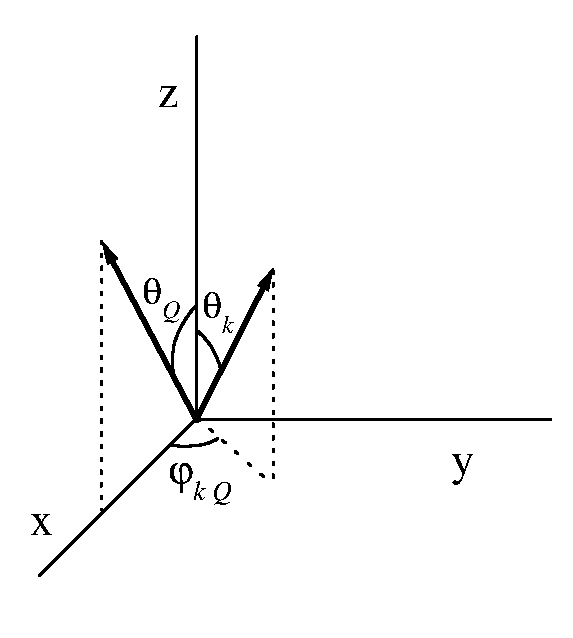
\includegraphics[height=7.5cm,clip,bb =55 495 309 760]{coord}
\caption{Definition of angles and planes used. \label{f:coord}}
\end{figure}

\begin{eqnarray} \label{Q:tdcs1}
\frac{d\sigma}{d E_{k} d\Omega_{k}d Q} &=&  m k \int
\frac{d\sigma}{d \bm{k} d \bm{Q} } d \Omega_{Q} \\
&=& m k \frac{(2 \pi)^{4}}{v}\int | t_{if}|^{2} \delta\left(
E_{i}-E_{f} \right) 2 \pi \, Q^{2} \, \sin \theta_{Q}\, d
\theta_{Q}\nonumber \\
&=& m k \frac{(2 \pi)^{5}\, Q^{2}}{v}\int | t_{if}| ^{2}
\delta\left(E_{i} - \frac{K^{2}_{j}} {2 \mu_{j} } - \frac{k^{2}_{j}}{2
m_{j} }\right) \sin \theta_{Q} \ d \theta \nonumber
\end{eqnarray}

  \noindent
Inserting $\bm{k}_{N}, \bm{K}_{N}$ as a function of $\bm{k}, \bm{Q}$ we
get for the argument of the delta function

\begin{equation}\label{Q:delta-kKN}
E_{i} - \left( \frac{K^{2}_{N}} {2 \mu_{N} } + \frac{\left| m_N \bm{v}
- \bm{Q} + (m_N/M_T) \bm{k} \right| ^{2}}{2 m_N }\right)
\end{equation}

  \noindent
Now, defining
\begin{equation}\label{Q:p-Qk}
\fbeq{ \bm{p} = (m_{N}/M_{T}) \bm{k} + m_{N} \bm{v}\,,}
\end{equation}
%
the conservation of the energy may be rewritten as
%
\begin{equation}\label{Q:Energ-conse-kQ}
E_{i} = \frac{K^{2}_{N}} {2 \mu_{N} } + \frac{| \bm{p} - \bm{Q}
| ^{2}}{2 m_{N}} = \frac{K^{2}_{N}} {2 \mu_{N} } + \frac{p^{2}}{2
m_{N}} + \frac{Q^{2}}{2 m_{N}} - \frac{\bm{p} \cdot \bm{Q}}{m_{N}}
\end{equation}
%
where $\bm{p} \cdot \bm{Q} \ =  Q \ \left(  p_x \sin{\theta_{Q} + p_{z}
\cos \theta_{Q} } \right)$.

We are ready to perform the integral in \ref{Q:delta-kKN} in the way
\[
\int f(x) \delta (g(x)) d x = \sum_{x} \frac{f(x)}{|
g'(x)| } \,.
\]
%
In our case, by defining
%
\[
  \fbeq{
 P_o = \frac{m_{N}}{Q} \left( \frac{K^{2}_{N}} {2 \mu_{N} }+
\frac{p^{2}}{2 m_{N}} + \frac{Q^{2}}{2 m_{N}} - E_{i} \right)
  }
\]
%
 we get
\[
g(\theta_Q) = \frac{Q}{m_{N}}(-P_{o} + \bm{p} \cdot \hat{Q}) =
\frac{Q}{m_{N}}(P_{o} + p_{x} \sin{(\theta_{Q})} + p_{z}
\cos{(\theta_{Q})})
\]
%
and
%
\[
g'(\theta_{Q}) = \frac{Q}{m_N} \left( p_{x} \cos \theta_{Q}  - p_{z}
\sin \theta_Q \right) \, ,
\] 
%
then the TDCS is given by
\begin{equation}\label{Q:5xsEkWkQ}
\fbeq{ \frac{d\sigma}{d E_{k} d\Omega_{k}d Q} =   \frac{(2
\pi)^{5} m k m_N\, Q}{v } \frac{ | t_{if}| ^{2}}{| p_{x}
\cot{\theta_Q} - p_{z} | }}
\end{equation}

Here $\theta_Q$ is the solution of the delta's argument $g(\theta_Q) =
0$. Explicitly,
$$
0 =  \bm{p} \cdot \hat{Q} - P_{o} =  p_{x} \sin{(\theta_{Q})} + p_{z}
\cos{(\theta_{Q})}  - P_{o} \nonumber \, .
$$
%
Then
%
\begin{eqnarray*}
&& \left( p_{z} -P_{o} \omega \right)^{2} = \left(- p_{x} \sqrt{(1
- \omega^{2})}\right)^2 \nonumber \\
&& P_{o}^{2} +  p_{z}^{2} \omega^{2} - 2 P_{o} p_{z} \omega = p_{x}^{2}
\left( 1 - \omega^{2}\right) \nonumber \\
\Rightarrow && (P_{o}^{2} - p_{x}^{2}) - 2 P_{o} p_{z} \; \omega +
(p_{z}^{2} + p_{x}^{2}) \; \omega^{2} = 0
  \, ,
\end{eqnarray*}
%
whose solutions are\footnote{Writing the result in this form, only the
`+' sign is valid. The `-' sign would be the correct result for
$\varphi_{k\,Q}' =2 \pi - \varphi_{k\,Q}$ such that
$\cos{\varphi_{k\,Q}}=\cos{\varphi_{k\,Q}'}$, but not for
$\varphi_{k\,Q}$.}
%
$$
\fbeq{\cos{(\theta_Q)}\, = \, \omega = \frac{P_{o} p_{z} {\pm} p_{x} \,
\sqrt{( p_{x}^{2} + p_{z}^{2} - P_{o}^{2} )}}{p_{x}^{2} + p_{z}^{2}}
\,} .
$$

\subsection{TDCS as a function of $\theta_{K}$, $E_{k}, \theta_{k}$
and $\varphi_{kK}$}

$$
\frac{d\sigma}{d E_{k} d\Omega_{k}d \Omega_{K}} = m k
\frac{(2 \pi)^{4}}{v}\int | t_{if}| ^{2} K^{2} \delta\left(
\frac{p^{2}_{N}} {2 m_{N} } - \frac{| \bm{K} - \bm{p}| ^{2}}{2
m_{N} }\right) \ d K
$$
%
with
\begin{equation}\label{Q:pN-defin}
    \fbeq{
p_{N} = \sqrt{2m_{N}\left( E_{i} - \frac{K_{N}^{2}}{2 \mu_{N}} \right)}
    }
\end{equation}
%
and
\begin{equation}\label{Q:p-defin}
   \fbeq{
\bm{p} = \left( m_{N}/M_{T}\right) \left(M_{P} \bm{v} - \bm{k} \right)
\, . }
\end{equation}
%
Then, we have
$$
 g(K) = \frac{-1}{2 m_{N}}\left( K^{2} + p^{2} - p_{N}^{2} - 2 \bm{K}
\cdot \bm{p} \right)
$$
and
$$
  g'(K) = \frac{- K + \bm{p} \cdot \hat{K}}{m_{N}} \,.
$$
%
The cross section is given by
\begin{equation}\label{Q:tdcsK}
    \fbeq{
\frac{d\sigma}{d E_{k} d\Omega_{k}d \Omega_{K}} = m k
\frac{(2 \pi)^{4}}{v} \, \frac{m_{N} K^{2}}{| K - \bm{p} \cdot
\hat{K}| } \, | t_{if}| ^{2}
    }
\end{equation}
%
where, by energy conservation,
\begin{equation}\label{Q:K-kQ}
\fbeq{K = \bm{p} \cdot \hat{K} {\pm} \sqrt{\left( \bm{p} \cdot \hat{K}
\right)^{2} + p_{N}^{2} - p^{2}} \,.
    }
\end{equation}

\subsection*{Approximated expressions}

When there is a large asymmetry between the electron and target mass
($m/M_{T} \ll 1$), $\bm{p} \approx m_N \bm{v}$ and the TDCS is given by
\begin{equation}\label{Q:5xsEkWkQapp}
\fbeq{ \frac{d\sigma}{d E_{k} d\Omega_{k}d Q} = \frac{(2
\pi)^{5} m k \, Q}{v^{2}} | t_{if}| ^{2}}
\end{equation}
%
where, for small values of $Q$, the polar angle is given by
$$
\cos{\theta_{Q}} \approx \frac{P_{o}}{m_{N} v} \ll 1 \, .
$$

The projectile scattering angle is \emph{approximately} proportional to
the transferred momentum by $\theta_{K} = Q/K$ ($K \approx M_{P} v$ is
the final projectile momentum). Then the TDCSs are simply related
$$
\frac{d\sigma}{d E_{k} d\Omega_{k}d \Omega_K} \approx
\frac{(M_{P} v)^{2}}{2 \pi \, Q} \frac{d\sigma}{d E_{k}
d\Omega_{k}d Q}
$$



\subsection{TDCS as a function of electron and transferred
momenta $\bi{k}$, $Q_{\parallel }, \bi{Q}_{\perp}$}

$$
\frac{d \sigma}{d \bm{k} d Q_{\parallel }} = \frac{(2
\pi)^{5}}{v} \int_{0}^{\infty} Q_{\perp} d Q_{\perp} |
t_{if}^{2}|  \; \delta \left( E_{i} - \frac{K_{j}^{2}}{2 \mu_{j}} -
\frac{k_{j}^{2}}{2 m_{j}}\right)
$$
%
By using
$$
  \fbeq{
\bm{p}= m_{N} \left( \bm{k}/M_{T} + \bm{v} \right)
  }
$$
%
as defined in \ref{Q:p-Qk} and
$$
p_{N} = \sqrt{2m_{N}\left( E_{i} - \frac{K_{N}^{2}}{2 \mu_{N}} \right)}
$$
%
we get for the argument of the delta function
%
$$
g(Q_{\perp}) = \frac{p_{N}^{2} - | \bm{p}- \bm{Q}| ^{2}}{2 m_{N}}
= \frac{p_{N}^{2} - p^{2} - Q^{2} + 2 \bm{p}\cdot \bm{Q}}{2 m_{N}}
$$
%
and then
$$
g'(Q_{\perp}) = \frac{1}{m_{N}}\left( - Q_{\perp} + \bm{p}_{\perp}
\right) \, .
$$

The TDCS is given by
%
\begin{equation}\label{Q:tdcsqpar}
  \fbeq{
\frac{d \sigma}{d \bm{k} d Q_{\parallel }} = \frac{(2
\pi)^{5}}{v} \frac{Q_{\perp} \, m_{N}}{| p_{\perp}- Q_{\perp} | }
\; | t_{if}| ^{2} }
\end{equation}
%
where $Q_{\perp}$ is the solution of a quadratic equation with
coefficient
$$
  \fbeq{
a=1\;, \quad b= - 2 p_{\perp} \;, \quad c= - \left( p_{N}^{2} - p^{2} -
Q_{\parallel }^{2} + 2 p_{\parallel } Q_{\parallel } \right)
  }
$$
%
given by
%
\begin{equation}\label{Q:qperp}
  \fbeq{
Q_{\perp} =  p_{\perp} {\pm} \sqrt{p_{\perp}^{2} + p_{N}^{2} - p^{2} -
Q_{| }^{2} + 2 p_{\parallel } Q_{\parallel }}
    }
\end{equation}
%
where only the `+' sign is valid. In particular, when $m/M_{T} \ll 1$
(atomic or molecular target), the perpendicular component of $\bm{p}$
is very small and
$$
Q_{\perp} \approx \sqrt{p_{N}^{2} - (m_{N} v)^{2} - Q_{\parallel
}^{2}} \,.
$$

The TDCS as a function of $Q_{\perp}$ is
%
\begin{equation}\label{Q:5xskQperp}
\frac{d \sigma}{d \bm{k} \, d \bm{Q}_{\perp}} = \frac{1}{2 \pi
Q_{\perp}} \frac{d \sigma}{d \bm{k} d Q_{\perp}} = \frac{(2
\pi)^{4}}{v} \, \int | t_{if}| ^{2} \; \delta \left( g(Q_{|
| }) \right) d Q_{\parallel }
\end{equation}
%
where, as before,
%
$$
g(Q_{\parallel }) = \frac{p_{N}^{2} - p^{2} - Q^{2} + 2 \bm{p}\cdot
\bm{Q}}{2 m_{N}} \, .
$$
%
The TDCS are then given by
\begin{equation}\label{Q:tdcsperp}
  \fbeq{
\frac{d \sigma}{d \bm{k} \, d \bm{Q}_{\perp}} = \frac{(2
\pi)^{4}}{v} \, \frac{m_{N}}{| p_{\parallel }- Q_{\parallel } |
}| t_{if}|^{2}
  }
\end{equation}
%
and
\begin{equation}\label{Q:tdcsperp1}
  \fbeq{
\frac{d \sigma}{d \bm{k} \, d Q_{\perp}} = \frac{(2
\pi)^{5}}{v} \, \frac{m_{N} Q_{\perp}}{| p_{\parallel }- Q_{|
| } | }| t_{if}| ^{2}
  }
\end{equation}
%
where $Q_{\parallel}$ the solution of a quadratic equation with
%
$$
  \fbeq{
a=1\;, \quad b= - 2 p_{\parallel } \;, \quad c= - \left( p_{N}^{2} -
p^{2} - Q_{\perp}^{2} + 2 p_{\perp} Q_{\perp} \right)
  }
$$
\begin{equation}\label{Q:qpar}
  \fbeq{
Q_{\parallel } =  p_{\parallel } {\pm} \sqrt{p_{\parallel }^{2} +
p_{N}^{2} - p^{2} - Q_{\perp}^{2} + 2 p_{\perp} Q_{\perp}}
    }
\end{equation}

\noindent
 The energy conservation can be rewritten by using the value of the
initial energy $E_{i}=\mu_{T} v^{2}/2 \, \varepsilon_{i}$. We obtain:

\begin{equation}\label{Q:EC1}
\bm{Q} \cdot \bm{v} + \frac{\bm{Q}\cdot \bm{k}}{M_{T}} - \frac{Q^{2}}{2
m_{N}} + \varepsilon_{i} - \frac{k^{2}}{2 m_{T}} = 0
\end{equation}
%
Then, $Q_{\parallel }$ can be obtained from a quadratic equation with
$$
a=\frac{1}{2 m_{N}} \, , \qquad b= -\left( v + \frac{k_{\parallel
}}{M_{T}} \right) \, , \qquad c= \frac{Q^{2}_{\perp}}{2 m_{N}} -
\frac{\bm{k}_{\perp} \cdot \bm{Q}_{\perp}}{M_{T}} - \varepsilon_{i} +
\frac{k^{2}}{2 m_{T}}
$$

\subsection{As a function of $ E_{k}, \theta_{k}, \varphi_{k,K_{R}},\theta_{K_{R}}$}

As in equation \ref{Q:tdcs1}, the cross section is given by

\begin{eqnarray} \label{Q:tdcs2}
\frac{d\sigma}{d E_{k} d\Omega_{k}d \Omega_{K_{R}}} &=& m k
\int
\frac{d\sigma}{d \bm{k} \, d \Omega_{K_{R}} } d K_{R} \\
&=& m k \frac{(2 \pi)^{4}}{v}\int | t_{if}| ^{2}
\delta\left(E_{i} - \frac{K^{2}_{j}} {2 \mu_{j} } - \frac{k^{2}_{j}}{2
m_{j} }\right) \, d K_{R} \, . \nonumber
\end{eqnarray}
%
Again we'll use the $(\bm{k}_N,\bm{K}_N)$ pair in the energy
conservation,
$$
E_{i} = \frac{K^{2}_{N}} {2 \mu_{N} } + \frac{\left| m_N \bm{v} -
\bm{K}_R + (m_N/M_T -1) \bm{k} \right|^{2}}{2 m_N } = \frac{K^{2}_{N}}
{2 \mu_{N} } + \frac{\left| m_N \bm{v} - \bm{K}_R - (m_N/M_P)\, \bm{k}
\right| ^{2}}{2 m_N }
$$
%
and define a vector
$$
\fbeq{\bm{p}=m_{N}(\bm{v} - \bm{k}/M_P).}
$$
%
Thus, defining
$$
P_o = \sqrt{{2 m_N} \left( E_{i} - \frac{K^{2}_{N}} {2 \mu_{N} }-
\frac{p^{2}}{2 m_{N}} \right)}
$$
the argument of the cross section is
$$
g(K_{R}) = \frac{1}{2 m_{N}} \left( P_o^{2} - K_{R}^{2} + 2 K_{R} \,
\hat{K}_{R} \cdot \bm{p} \right)
$$
and the derivative
$$
g'(K_{R}) = \frac{1}{m_{N}} \left(K_{R} - \bm{p} \cdot \hat{K}_{R}
\right)
$$

Then, the cross section is given by
\begin{equation}\label{Q:5xsEkWkWR}
  \fbeq{
\frac{d\sigma}{d E_{k} d\Omega_{k}d \Omega_{K_{R}}} =
\frac{(2 \pi)^{4} m k m_N}{v } \frac{ | t_{if}| ^{2}}{|  K_{R}
- \bm{p} \cdot \hat{K}_{R} | }
    }
\end{equation}
%
where the value of the $K_{R}$ modulus is fixed by energy conservation
$g(K_{R})=0$. Explicitly\footnote{Only the + sign is valid because
$K_{R}$ is defined positive},

\begin{equation}\label{Q:KR-k}
  \fbeq{
K_{R} =  \bm{p}\cdot \hat{K}_{R} {\pm} \sqrt{\left( \bm{p}\cdot \hat{K}_{R}
\right)^{2} + P_o^2}
  }
\end{equation}
%
with
$$
\bm{p}\cdot \hat{K}_{R} = p_{x} \sin{\theta_{R}} + p_{z}
\cos{\theta_{R}}
$$

\newpage
\subsection{As a function of $\bi{k}$, $K_{R \perp}$ ($K_{R \parallel }$)}
Closely related to the usual presentation of COLTRIMS results are the
cross sections
\begin{equation} \label{Q:tdcsxsr0}
\frac{d \sigma}{d \bm{k} \, d K_{R \perp}} = \frac{(2
\pi)^{4}}{v} \,(2 \pi K_{R \perp}) \int d K_{R | }, \parallel
t_{if}\parallel ^{2} \delta \left( E_{i} - E_{f} \right)
\end{equation}
%
and
\begin{equation}\label{Q:5xskR}
\frac{d \sigma}{d \bm{k} \, d K_{R \parallel }} = \frac{(2
\pi)^{4}}{v} \, \int d \bm{K}_{R \perp} \, | t_{if}| ^{2}
\delta \left( E_{i} - E_{f} \right) \, .
\end{equation}


In particular, for the first of them (eq. \ref{Q:tdcsxsr0}), we write
the conservation of the energy as $g(K_{R \perp}) = 0$, with
$$
g(K_{R \perp}) = \frac{1}{2 m_{N}} \left( P_o^{2} - K_{R | }^{2}
  - K_{R \perp}^{2} + 2 \bm{K}_{R} \cdot \bm{p} \right)
$$
and then
$$
g'(K_{R \perp}) = \frac{1}{m_{N}} \left( p_{\parallel } - K_{R \parallel }
\right) \,
$$
where $\bm{p} = m_{N}\left( \bm{v} - \bm{k}/M_{P}\right)$.

The cross section can be written
\begin{equation}\label{Q:tdcsxyr}
  \fbeq{
\frac{d \sigma}{d \bm{k} \, d K_{R \perp}} = \frac{(2
\pi)^{5}\,m_{N} \, K_{R \perp}}{v} \, \frac{ | t_{if}| ^{2}
}{| p_{\parallel } - K_{R | }| }
  }
\end{equation}
%
where, by energy conservation, $K_{R | }$ is the solution of a
quadratic equation with
%
$$
  \fbeq{
a=1 \qquad,\quad b = -2 p_{\parallel } \qquad \mbox{and} \quad c= -
\left( P_{o}^{2} + 2 K_{R \perp} p_{\perp} - K_{R\perp}^{2} \right)
  }
$$

%%%%%%%%%%%%%%%%%%%%%%%%%%%%%%%%%%%%%%%%%%%%%%%%%%%%%%%%%%%%%%%%%%%%%%%

\subsection{As a function of $\bi{K}_{R}$, $Q_{R \perp}$($Q_{R | }$)}

The energy conservation equation can be written,

\begin{equation}\label{Q:EC2}
\bm{Q} \cdot \textbf{v} + \frac{\bm{Q}\cdot \bm{K}_{R | }}{m} -
\frac{Q^{2}}{2 m_{P}} + \varepsilon_{i} - \frac{K^{2}_{R}}{2 m_{T}} = 0
\ .
\end{equation}

\noindent Taking into account the symmetry between $m$ and $M_{T}$, the
result is the same that for $d\sigma/d \bm{Q}_{\perp} d
\bm{k}$ but exchanging the role of electron and target-ion.

\subsection{As a function of $E_{k}$, $\theta_{R}$,
$\varphi_{Q,R}$, $Q_{\perp}$: { \texttt{Approximated expressions}}}

We calculate this TDCS as

$$
\frac{d\sigma}{d Q_{\perp} d E_k d \varphi_{Q,R} d
\theta_{K_{R}}} = \mathcal{J}_{o} \ \frac{K_{R}^{2}}{k/m} \,
\frac{d\sigma}{d Q_{\perp} d \bm{K}_{R}}
$$
%
where the Jacobian of the transformation is defined as
$$
\mathcal{J}_{o} = \frac{\partial \left( Q_{\perp}, \Omega_{\bm{K}_{R}}
, \ k \; \right) }{\partial \left( Q_{\perp}, \Omega_{\bm{K}_{R}} ,
K_{R} \right)} \ .
$$

In order to evaluate the Jacobian we write
%
\begin{equation}\label{Q:k-KR}
k^{2} = | \bm{Q} - \bm{K}_{R}| ^{2} = Q^{2} + K_{R}^{2} - 2 K_{R}
\left( Q_{\parallel } \cos{\theta_{K_{R}}} + Q_{\perp}
\sin{\theta_{K_{R}}} \cos{\varphi_{Q,R}}\right).
\end{equation}
%
Differentiating implicitly we find,

$$
\left( \frac{\partial K_{R}}{\partial k }\right)_{Q_{\perp},\,
  \Omega_{K_{R}}} =
\frac{ k - \left( Q_{\parallel } - K_{R} \cos{\theta_{K_{R}}}
\right)\displaystyle{ \left( \frac{\partial Q_{\parallel }}{\partial k
}\right)_{Q_{\perp},\, \Omega_{K_{R}}}}} {K_{R}- Q_{\parallel }
\cos{\theta_{K_{R}}} - Q_{\perp} \sin{\theta_{K_{R}}}
\cos{\varphi_{Q,R}} }
$$

\noindent
Here the magnitude of the recoil momentum is the solution of the second
order equation \ref{Q:KR-k}, with coefficients
$$
a=1 \quad  , \qquad b=-2 \left( Q_{\parallel } \cos{\theta_{K_{R}}} +
Q_{\perp} \sin{\theta_{K_{R}}} \cos{\varphi_{Q,R}}\right) \quad ,
\qquad c = Q^{2} - k^{2}
$$

  \noindent
where, in the approximation of heavy masses for the target and the
projectile, we have
$$
Q_{\parallel } = \frac{k^{2}/2m + | \varepsilon_{i}| }{v} \qquad
\qquad \Rightarrow \qquad \left( \frac{\partial Q_{\parallel
}}{\partial k }\right)_{Q_{\perp},\, \Omega_{K_{R}}} = \frac{k}{mv}
$$

\subsection{As a function of the P-e center of mass momentum}
\label{S:as-function-p}
Here we derive the cross section in terms of the pair of relative momenta: $(\bm{k}_{P}, \bm{k}_{P,cm})$, where $\bm{k}_{P,cm}$ is the momentum of the center of mass of the projectile-electron system.
From momentum conservation, we have $M_{P} \bm{v} = \bm{k}_{P,cm} + \bm{K}_{R}$, then:
$$
\bm{k}_{P,cm}= \bm{K}_{P} + \mu_{P}\frac{M_{P}}{M_{T}}\, \bm{v}
$$
We are interested in the following cross section:
$$
\frac{d \sigma}{d \bm{k}_{P} d \hat{k}_{P,cm}} = \frac{(2 \pi)^{4}}{v} \int |t_{if}|^{2} \delta \left( \frac{p_{p}^{2}}{2 m_{P}} - \frac{|\bm{k}_{P,cm} - \bm{p}|^{2}}{2 \mu_{P}} \right)
$$
%
where 
$$
p_{p}= \sqrt{2 \mu_{P}(E_{i}-\frac{k_{P}^{2}}{2 m_{P}})} \quad,\qquad \bm{p}=  \mu_{P}\frac{M_{P}}{M_{T}}\, \bm{v}
$$

Then, with the notation used above, we have
\begin{eqnarray*}
g(k_{P,cm})&=& - \frac{k_{P,cm}^{2}}{2 \mu_{P}} + k_{P,cm}\frac{\hat{k}_{P,cm} \cdot \bm{p}}{\mu_{P}} + \left( \frac{p_{P}^{2}}{2 \mu_{P}} - \frac{p^{2}}{2 \mu_{P}}\right) \\
g'(k_{P,cm})&=& \frac{1}{\mu_{P}}\left(  \hat{k}_{P,cm} \cdot \bm{p} - k_{P,cm} \right)
\end{eqnarray*}

Then, the desired cross section can be written as:
\begin{equation}\label{Q:xs-pe-cm}
  \frac{d \sigma}{d \bm{k}_{P} d \hat{k}_{P,cm}} = \frac{(2 \pi)^{4}\mu_{P} k^{2}_{P,cm} }{v}\frac{ |t_{if}|^{2}}{|\hat{k}_{P,cm} \cdot \bm{p} - k_{P,cm}|}
\end{equation}
%
where the magnitude of the vector is the solution of a quadratic equation with
$$
a=1 \quad  , \qquad b=-2 \left(\hat{k}_{P,cm} \cdot \bm{p} \right) \quad ,
\qquad c = p^{2} - p_{P}^{2}
$$

Observe that for light projectiles ($M_{P} \ll M_{T}$) the above expression may be simplified. The momentum $\bm{p}$ may be neglected in the denominator and the cross sections reads:
\begin{equation}\label{Q:xs-pe-cm-app}
  \frac{d \sigma}{d \bm{k}_{P} d \hat{k}_{P,cm}} \approx \frac{(2
    \pi)^{4}\mu_{P} k_{P,cm} }{v} \, |t_{if}|^{2} \quad ,  \qquad k_{P,cm}
  \approx p_{P}  
\end{equation}

The relation between the laboratory momenta and the relative and two-body center of mass momenta is
\[
\bm{k}= \bm{k}_{P} + \frac{m_{P}}{M_{P}}\bm{k}_{P,cm} \qquad \, \qquad
\bm{k}= -\bm{k}_{P} + \frac{m_{P}}{m}\bm{k}_{P,cm} 
\]
\section{Limit values of variables}
\label{S:Limit-value-varia}

Now we will obtain the minimum momentum transfer for a given value of
the electron momentum $\bm{k}$. We rewrite and simplify equation
\ref{Q:Energ-conse-kQ},

\begin{equation}\label{Q:Energ-conse-kQ-1}
p_{N} = \left| \bm{p} - \bm{Q} \right|
\end{equation}
%
where $p$ and $p_{N}$, given by equations \ref{Q:pN-defin} and
\ref{Q:p-defin}, depend on $\bm{k}$
\begin{eqnarray*}
\bm{p} &=& \left( m_{N}/M_{T}\right) \left(M_{P} \bm{v} - \bm{k}
\right)
\\
p_{N} &=& \sqrt{2m_{N}\left( E_{i} - \frac{K_{N}^{2}}{2
\mu_{N}} \right)}\, .
\end{eqnarray*}

This is the equation of a sphere centered in the momentum $\bm{p}$ and
with radius $p_{N}$. The minimum $Q$ corresponds to the vector that is
in the direction of $\bm{p}$ and the value is just the difference
between the center and the radius
%
\begin{equation}\label{Q:Qmin-k}
Q_{min} = |p_{N} - p| =  \sqrt{2m_{N}\left( E_{i} - \frac{K_{N}^{2}}{2
\mu_{N}} \right)} - \left( m_{N}/M_{T}\right) \left| M_{P} \bm{v} -
\bm{k} \right|
\end{equation}


\noindent To get it from the above equations we take squares in
equation \ref{Q:Energ-conse-kQ-1} to obtain a quadratic equation
$$
Q^{2} - 2 p\, Q \cos{\theta_{Q,p}} - \left( p_{N}^{2} - p^{2} \right) =
0 \, ,
$$
with positive solution
$$
Q = p\, \cos{\theta_{Q,p}} + \sqrt{(p\, \cos{\theta_{Q,p}})^{2} +
\left( p_{N}^{2} - p^{2} \right)} \, .
$$
%
The minimum value  given by \ref{Q:Qmin-k} corresponds to
$\theta_{Q,p}=\pi$.

The relation between the pairs $(\bm{k}_{P,cm}, \bm{k}_{P})$ and $(\bm{k},
\bm{Q})$ can be easily obtained by deriving the corresponding relations between
coordinates
\begin{eqnarray*}
  \bm{k}&=& \frac{m}{m+ M_{P}}\bm{k}_{P,cm} + \frac{m}{M_{P}}\bm{k}_{P} \\
  \bm{Q}&=& M_{P} \bm{v} - \frac{m}{m+ M_{P}}\bm{k}_{P,cm} + \bm{k}_{P}
\end{eqnarray*}


\section{Double differential cross sections}

The double differential cross section (DDCS) in the momentum of each
particle can be obtained by integrating the TDCS


\subsection{DDCS in the momentum $\bi{k}$ of the electron}

\begin{eqnarray*}
\frac{d \sigma}{d \bm{k}} &=& \int_{Q^{-}}^{Q^{+}} d Q
\int_{0}^{2 \pi} d \varphi \, \frac{d\sigma}{d \bm{k} \, d
Q d \varphi} \qquad  \qquad \mbox{with } \qquad Q^{\pm}= k_{N} {\pm} p
\\
&=& \int_{Q_{\parallel }^{-}}^{Q_{\parallel }^{+}} d Q_{\parallel
} \frac{d\sigma}{d \bm{k} \, d Q_{\parallel }}  \qquad \quad
\qquad \mbox{with }  \qquad \qquad Q^{\pm}_{\parallel } = k_{N} {\pm} p_{|
| }
\\
&=& 2 \pi \int_{0}^{Q_{\perp}^{+}} Q_{\perp} d Q_{\perp}
\frac{d\sigma}{d \bm{k} \, d \bm{Q}_{\perp}} \qquad \mbox{with
} \qquad\qquad Q_{\perp}^{\pm}= k_{N} {\pm} p_{\perp}
\end{eqnarray*}

We will now make explicit the evaluation given by the first of these
equations. The quintuple differential cross section


\subsection{Note on the evaluation of total cross sections}

The total cross section is obtained by integrating the single
differential cross section in electron energy. In the case of heavy
projectiles, the maximum electron energy is huge and, for every
practical use, indistinguishable from infinity. In the case of light
projectiles, while the recoil ion remains virtually at rest, its energy
can be neglected. Thus, the maximum electron energy would correspond to
the total energy ( electron-target binding energy subtracted to the
initial projectile kinetic energy). However, in a real calculation the
infinity limit is not practicable and the domain of integration must be
contained in a finite region. In many cases this limit will extend to a
few atomic units of energy. A good estimation of the energy becomes
numerically important when the integrand is expensive to compute. In
order to estimate the maximum electron energy which contributes
appreciable to the total cross section we use a classical
approximation.

The simplest, classical binary projectile-electron collision was
considered first by Thompson \parencite{Thomson1912PMp449}. This approximation
considers that the electron is initially at rest and that the target
nucleus only provides the binding energy. Within this approximation the
single differential cross section is given by
\begin{equation}\label{Q:Thomson}
\frac{d \sigma}{d (\Delta E)} = \frac{2 \pi Z_{P}^{2}}{m v^{2}
(\Delta E)^{2}}
\end{equation}
%
where
$$
\Delta E = I_{0} + E_{k}
$$
with $I_{0}=| \varepsilon_{i} | $. The total cross section in
this approximation is given by
$$
\sigma \equiv \sigma_{E_{0}} = \int_{I_{0}}^{E_{0}} \frac{d
\sigma}{d (\Delta E)} \,d (\Delta E) \,,
$$
where
$$
E_{0}= \frac{1}{2} (2 \,m_{P}\, v)^{2}
$$


\noindent Given the accuracy $\epsilon_{r}>0$, the upper limit
$E_{cut}$ in the integral in energy must verify
\[
  (\sigma - \sigma_{E_{cut}}) = \epsilon_{r} \, \sigma
\]

Inserting expression \ref{Q:Thomson} we obtain
\begin{equation}\label{Q:E-cut}
 \Delta E_{cut} = \frac{I_{0}/E_{0}}{\epsilon_{r} + I_{0}/E_{0}}\; E_{0}
\end{equation}

Thus, the cut energy is

$$
E_{cut} = I_{0}\left(\frac{1}{\epsilon_{r} + (I_{0}/E)} - 1 \right)
$$

\subsection{Change of variables}

The above estimation gives us an important clue. The dependence of the
single differential cross section with the electron energy (eq.
\ref{Q:Thomson}) can be used to improve numerical convergence. We write
the cross section as the product of a (unknown but smooth) function
$g(\Delta E)$ and $(\Delta E)^{-2}$
$$
\sigma = \int_{I_{0}}^{\Delta E_{cut}} \frac{d \sigma}{d (\Delta
E)}\, d (\Delta E) = \int_{I_{0}}^{\Delta E_{cut}} d (\Delta E)
\, \frac{g(\Delta E)}{(\Delta E)^{2}}
$$

Changing variables in the integral ($u=(\Delta E)^{-1}$), ($d u =
-(\Delta E)^{-2}\, d (\Delta E)$) we can write
$$
\sigma = \int_{1/\Delta E_{cut}}^{1/I_{0}}g(1/u) \; d u
$$
%
where $g(1/u)= (\Delta E)^{2} \, d \sigma / d (\Delta E)$.

%%% Local Variables: 
%%% mode: latex
%%% TeX-master: "main"
%%% End: 

\chapter{CDW Approximations}

\section{CDW wavefunction}
We will use the final state wavefunction $C_{3}$ o CDW:
%
\begin{equation}\label{Q:C3}
\Psi^{\pm}_{C3} (\vect{r},\vect{R}) = \frac{e^{i (\vect{k}_j\cdot
\vect{r}_j+\vect{K}_j\cdot \vect{R}_j)}}{(2 \pi)^3} \,
D^{\pm}(\nu_T,\vect{k}_T,\vect{r}_T) \, D^{\pm}(\nu_P,\vect{k}_P,\vect{r}_P)
\,D^{\pm}(\nu_N,\vect{k}_N,\vect{r}_N)
\end{equation}
%
where the distortion factor $D^{\pm}$ are defined in terms of the two body
wave functions as
\[
 \psi^{\pm}_{\vect{k}_j}(\vect{r}_j)  = (2\pi)^{-3/2}e^{i \vect{k}_{j}
 \cdot \vect{r}_{j}} D^{\pm}(\nu_j,\vect{k}_{j},\vect{r}_{j})
\]
%
For a continuum state with Coulomb interactions the distortion factor
is given by
%
\begin{equation}\label{Q:DFactCoul}
 D^{\pm}(\nu_j,\vect{k}_{j},\vect{r}_{j})= N^{\pm}(\nu_{j}) \,{_1F_1}\left(
\mp i \nu_{j};1; {\pm} i (k_{j} r_{j} \mp \vect{k}_{j} \cdot\vect{r}_{j}
) \right) \, ,
\end{equation}
%
$N^{\pm}(\nu_j)= \Gamma(1 {\pm} i\nu_j) e^{-\pi \nu_j/2}$ and the
Sommerfeld's parameter $\nu_j = m_j Z_j/ k_j$.

In the general case, for arbitrary interaction between particles it can
be defined as
\begin{equation}\label{Q:DFact}
D^{\pm}(\nu_j,\vect{k}_j,\vect{r}_j)  = (2\pi)^{3/2}e^{ - i\vect{k}_j \cdot
\vect{r}_j} \psi^{\pm}_{\vect{k}_j}(\vect{r}_j)
\end{equation}
where $\psi^{\pm}_{\vect{k}_j}(\vect{r}_j)$ is the exact two-body wavefunction.


\section{CDW-Born approximation}

We use the final state $\Psi_{C3}$ and an initial undistorted Born wave
function $\Psi_{B1}=\phi_{T} \, \exp{ \left( i \mu_{T} \vect{v}_{T}
\cdot \vect{R}_{T} \right)}$. The wavefunction is the C3
\begin{equation} \label{Q:FCC1}
\Psi^{\pm}_{C3} (\vect{r},\vect{R}) = \frac{e^{i {\bf k}_j\cdot {\bf r}_j+{\bf
K}_j\cdot {\bf R}_j}}{(2 \pi)^3} \, D^{\pm}(\nu_T,{\bf k}_T,{\bf r}_T) \,
D^{\pm}(\nu_P,{\bf k}_P,{\bf r}_P) \,D^{\pm}(\nu_N,{\bf k}_N,{\bf r}_N)
\end{equation}

Here the Coulomb wave function is
\begin{equation}\label{Q:FCC} 
\psi^{\pm}_{{\bf k}_j}({\bf r}_j)  = (2\pi)^{-3/2}e^{i{\bf
k}_j \cdot {\bf r}_j} D^{\pm}(\nu_j,{\bf k}_j,{\bf r}_j)
\end{equation}
%
with
%
\begin{eqnarray}\label{Q:NNorm}
D^{\pm}(\nu_j,{\bf k}_j,{\bf r}_j) &=& N(\nu_j) \,{_1F_1}\left( \mp i
\nu_j;1; {\pm} i(k_j r_j \mp {\bf k}_j\cdot{\bf r}_j ) \right) \, ,\\
\nonumber \\ 
 N^{\pm}(\nu_j)&=& \Gamma(1 {\pm} i\nu_j)\, e^{-\pi \nu_j/2}
\end{eqnarray}
%
and the Sommerfeld's parameter $\nu_j = m_j Z_j/ k_j$.

\subsection{T-matrix in prior-form}
In the prior-form the final distortion, given by the channel potential
is equal to $V_{P} + V_{N}$. We can separate the T-matrix in the form:
$t_{if} = t_{P} + t_{N}$, with $t_{j} = \langle \Psi_{f}^{-}\mid
V_j\mid \Psi_{i} \rangle $

\begin{eqnarray} \label{QA2:6}
t_{P} = \frac{Z_{P}}{(2 \pi)^{3}} && \int d \vect{r}_{P} \,
   \frac{e^{- i \, \vect{Q} \cdot \vect{r}_{P}}}{\vect{r}_{P}}
D^{-\,\ast}(\nu_{P},\vect{k}_{P},\vect{r}_{P}) {\times}
\\
& & \int d \vect{r}_{T} \, e^{i \, (m_{T}/m) \, \vect{Q} \cdot
\vect{r}_T} \, \phi_{i}(\vect{r}_T) \, \phi^{-\, \ast}_{f}(\vect{r}_T) \,
D^{-\,\ast}(\nu_{N}, \vect{k}_{N}, \vect{r}_{T} - \vect{r}_{P} ) \;,
\nonumber
\end{eqnarray}
%
for the projectile-electron interaction and
%
\begin{eqnarray}\label{QA2:7}
t_{N} = \frac{Z_{N}}{(2 \pi)^{3}} & & \int d \vect{r}_{N} \,
   \frac{e^{ i \, \vect{Q} \cdot \vect{r}_{N}}}{\vect{r}_{N}}
D^{-\,\ast}(\nu_{N},\vect{k}_{N},\vect{r}_{N}) {\times}
\\
 & & \int d \vect{r}_T \,
e^{- i \, (m_{T}/M_{T}) \, \vect{Q} \cdot \vect{r}_T} \,
\phi_{i}(\vect{r}_{T})\, \phi^{-\, \ast}_{f}(\vect{r}_T) \,
D^{-\,\ast}(\nu_{P}, \vect{k}_{P}, \vect{r}_{T} - \vect{r}_{N} ) \nonumber
\end{eqnarray}
for the internuclear perturbation.

We define the atomic form factor $\langle \phi_{f}\mid e^{i
\vect{p}\cdot \vect{r}}\mid \phi_{i} \rangle$
%
\begin{equation}\label{QA2:8}
  F_{if}(\vect{p}) = \frac{1}{(2 \pi)^{3/2}} \int d \vect{r}_{T} \;
e^{\, i \vect{p} \cdot \vect{r}_{T}} \, \phi_{i}(\vect{r}_{T}) \,
\phi^{-\, \ast}_{f}(\vect{r}_T)
\end{equation}
%
such that
\[
\phi_{i}(\vect{r}) \, \phi^{-\, \ast}_{f}(\vect{r}) = \frac{1}{(2
\pi)^{3/2}} \int d \vect{p} \, e^{- i \vect{p} \cdot \vect{r}} \,
F_{if}(\vect{p}) \,.
\]
%
Replacing in \ref{QA2:6} and \ref{QA2:7} we get
%
\begin{eqnarray}\label{QA2:9}%
t_{P} &=& -\frac{Z_{P}\, \mathcal{N}_{P} \mathcal{N}_{N}}{(2\pi)^{9/2}}
\; \lim_{\lambda_{1},\lambda_{2} \to 0^{+}} \mathcal{H} \left(
\lambda_{1},- \nu_{P},\vect{k}_{P} ;  \lambda_{2},-
\nu_{N},\vect{k}_{N};\vect{Q} , -(m_{T}/M_{T}) \, \vect{Q} \right)
  \nonumber \\
t_{N} &=& \frac{Z_{N} \, \mathcal{N}_{P} \mathcal{N}_{N}}{(2\pi)^{9/2}}
\; \lim_{\lambda_{1},\lambda_{2} \to 0^{+}} \mathcal{H} \left(
\lambda_{1}, - \nu_{N},\vect{k}_{N} ; \lambda_{2},- \nu_{P},\vect{k}_{P} ;
- \vect{Q} ,  (m_{T}/m) \, \vect{Q} \right) \; ,
\end{eqnarray}
%
with
%
\begin{equation}\label{QA2:10}%
 \mathcal{H} \left( \lambda_{1},a_{1},\vect{k}_{1} ;
  \lambda_{2},a_{2},\vect{k}_{2}; \vect{Q}, \vect{p} \right)  =
 \int d \vect{q} \; F_{if}( \vect{p} - \vect{q} ) \;
 J_{0}( \lambda_{2}, \vect{q} + \vect{Q}, a_{2}, \vect{k}_{2} ) \;
 J_{1}( \lambda_{1}, \vect{q}, a_{1}, \vect{k}_{1} )
\end{equation}
%
where $J_{0}$ y $J_{1}$ are the Nordsieck-like integrals
\parencite*{Nordsie1954PRp785} given by eq.~\ref{Q:Jint}.

Now, because the $J_{o}$ is more peaked in the origin than $J_{1}$,
will be useful to change variables $\vect{q} \to \vect{q}' = \vect{q} +
\vect{Q}$ and get (dropping the prime)
\begin{equation}\label{QA2:12}%
 \mathcal{H} \left( \lambda_{1},a_{1},\vect{k}_{1} ;
  \lambda_{2},a_{2},\vect{k}_{2}; \vect{Q}, \vect{p} \right)  =
 \int d \vect{q} \; F_{if}( \vect{p} + \vect{Q} - \vect{q} ) \;
 J_{0}( \lambda_{2}, \vect{q} , a_{2}, \vect{k}_{2} ) \;
 J_{1}( \lambda_{1}, \vect{q} - \vect{Q}, a_{1}, \vect{k}_{1} )
\end{equation}

We can also write simply
\begin{align*}
  t_{if}&= \frac{1}{(2 \pi)^{9/2}} \int d \vect{p}\, F_{if}(\vect{p})\,\Big[ Z_{N} J_{1}(0^{+}, \vect{k}_{1},-\nu_{N}, \vect{k}_{N}) J_{0}(0^{+}, \vect{k}_{2},-\nu_{P}, \vect{k}_{P}) - Z_{P}\,  J_{0}(0^{+}, \vect{k}_{1},-\nu_{N}, \vect{k}_{N}) J_{1}(0^{+}, \vect{k}_{2},-\nu_{P}, \vect{k}_{P}) \Big]
\intertext{with}
\vect{k}_{1}&= \frac{m_{T}}{m}\vect{Q} - \vect{p} \\
\vect{k}_{2}&= - \left( \frac{m_{T}}{M_{T}}\vect{Q} + \vect{p}  \right)
\end{align*}

\subsection{Series expansion of the T-matrix}

We expand the atomic form factor $F_{if}$ in a Taylor series around the
point $\vect{q}= \vect{Q}$, where $J_{1}$ present its maximum,

\begin{equation}\label{QTaylorFif}
F_{if}(\vect{p} + \vect{Q} - \vect{q}) = F_{if}(\vect{p}) + \left( \vect{Q} -
\vect{q} \right) \cdot \left. \nabla F_{if} \right| _{\vect{p}} +
\Delta^{2} F_{if}
\end{equation}

We obtain a similar expansion for $\mathcal{H} = \mathcal{H}_{o} +
\mathcal{H}_{1} + \Delta^{2} \mathcal{H}$.

\subsection*{Evaluation of $\mathcal{H}_{o}$}
We evaluate the first term as:
%
\begin{equation}\label{Q:mathc-lambd-a_1-1}
 \mathcal{H}_{o}\left( \lambda_{1},a_{1},\vect{k}_{1} ;
\lambda_{2},a_{2},\vect{k}_{2}; \vect{Q}, \vect{p} \right) = F_{if}(\vect{p})
\int J_{o}(\lambda_{2},\vect{q},a_{2},\vect{k}_{2}) \, J_{1}(\lambda_{1},
\vect{q}- \vect{Q} ,a_{1},\vect{k}_{1} ) \, d \vect{q}
\end{equation}

By using the relation \ref{Q-N1-Jb} we obtain
\begin{equation}\label{Q:fbeq-mathcalh_o}
  \fbeq{
\mathcal{H}_{o} \left( \lambda_{1},a_{1},\vect{k}_{1} ; \lambda_{2},
a_{2}, \vect{k}_{2} ; \vect{Q}, \vect{p} \right) = (2 \pi)^{3} \;
F_{if}(\vect{p}) \; N_{1} \left(\lambda_{1}+\lambda_{2}, \vect{Q} ; a_{1},
- \vect{k}_{1} ; a_{2}, \vect{k}_{2} \right) \, ,
  }
\end{equation}
%
where $N_{1}$ is the Nordsieck's Integral defined in \ref{Q:N1}.

\subsection*{The order 1}
%
\begin{eqnarray}\label{Q:order1}
 \mathcal{H}_{1}\left( \lambda_{1},a_{1},\vect{k}_{1} ;
\lambda_{2}, a_{2}, \vect{k}_{2}; \vect{Q}, \vect{p} \right) &=&  \nabla
F_{if} ({\vect{p}}) \cdot  \left[ \int \left( \vect{Q} - \vect{q} \right)
J_{o}(\lambda_{2},\vect{q},a_{2},\vect{k}_{2}) \,  J_{1}(\lambda_{1},
\vect{q}- \vect{Q} ,a_{1},\vect{k}_{1} ) \, d \vect{q} \right]
\end{eqnarray}

  \noindent
Now, while $\nabla F_{if} ({\vect{p}}) = i \, \vect{L}_{if}(\vect{p})$ and
using $\vect{I}_{1}$ as in eq. \ref{Q-N1-Jc} we obtain

\begin{eqnarray*}
&&\mathcal{H}_{1}\left( \lambda_{1},a_{1},\vect{k}_{1} ; \lambda_{2},
a_{2}, \vect{k}_{2}; \vect{Q}, \vect{p} \right)= \\
&&\qquad i \vect{L}_{if} ({\vect{p}})
\cdot \left[(2 \pi)^{3} \vect{Q} N_{1}(\lambda,\vect{Q} ; a_{1},-\vect{k}_{1}
; a_{2},\vect{k}_{2}) - \frac{(2 \pi)^{3}}{-i}
\vect{I}_{1}(\lambda,\vect{Q}; a_{1},-\vect{k}_{1}; a_{2},\vect{k}_{2} )
\vstretch \right]
\end{eqnarray*}

The first order is then given by
\begin{eqnarray}\label{Q:mathc-lambd-a_1}
&&\mathcal{H}_{1}\left( \lambda_{1},a_{1},\vect{k}_{1} ; \lambda_{2},
a_{2}, \vect{k}_{2}; \vect{Q}, \vect{p} \right)= \\
&& \qquad (2 \pi)^{3} \, \vect{L}_{if}
({\vect{p}}) \cdot  \left[ \vect{I}_{1}(\lambda,\vect{Q}; a_{1},-\vect{k}_{1};
a_{2},\vect{k}_{2} ) + i \vect{Q} N_{1}(\lambda,\vect{Q} ;
a_{1},-\vect{k}_{1} ; a_{2},\vect{k}_{2}) \vstretch \right] \nonumber
\end{eqnarray}
%
where $\lambda = \lambda_{1}+\lambda_{2}$.



\section{CDW Final Distortion potential}
The wavefunction \ref{Q:C3}, with $D$ defined as in \ref{Q:DFactCoul},
has been employed as an approximated solution of the three-body Coulomb
continuum state. Although our interest is focused in the Coulomb case,
this wavefunction can be defined for general interactions between the
particles through \ref{Q:C3} and \ref{Q:DFact}.

To determine the distortion potential we write the wavefunction as
\[
\Psi^{\pm}_{C3} (\vect{r},\vect{R}) = \frac{e^{i \vect{k}_j\cdot
\vect{r}_j+\vect{K}_j\cdot \vect{R}_j}}{(2 \pi)^3} D_{T} \,
\pounds(\vect{r},\vect{R})
\]
where, in order to simplify the notation, we write $D^{\pm}_{j} \equiv
D^{\pm}(\nu_j,\vect{k}_{j},\vect{r}_{j})$.

\begin{equation}\label{Q:C3-final-disto}
\left( H - E \right) \Psi(\vect{r}_{j}, \vect{R}_{j}) = \left[ H_{0} +
V_{T}(\vect{r}_{T}) + V_{P}(\vect{r}_{P}) + V_{N}(\vect{r}_{N}) - E \right]
\left[ \frac{e^{i (\vect{k}_j\cdot \vect{r}_j+\vect{K}_j \cdot
\vect{R}_j)}}{(2 \pi)^3} \, D_{T} \, \pounds(\vect{r},\vect{R}) \right]
\end{equation}

\noindent Now, using that
\begin{eqnarray*}
\nabla^{2}_{\vect{r}}(f \, g) &=& f \, \nabla^{2}_{\vect{r}}(g) + g \,
\nabla^{2}_{\vect{r}}(f) + 2 \overrightarrow{\nabla}_{\vect{r}}(g) \cdot
\overrightarrow{\nabla}_{\vect{r}}(f) \, , \\
\overrightarrow{\nabla}_{\vect{r}} e^{i \vect{k}\cdot \vect{r}} &=&
i \,
\vect{k} \, e^{i \vect{k}\cdot \vect{r}} \, , \\
\overrightarrow{\nabla}_{\vect{R}_{T}} D_{T}(\vect{r}_{T}) &=& 0
\end{eqnarray*}
 we obtain
%
\begin{eqnarray*}
\left( H - E \right) \Psi &=& \left( \frac{k_{T}^{2}}{2m_{T}} +
\frac{K_{T}^{2}}{2 \mu_{T}} - E \right) \Psi + \frac{e^{ i
(\vect{k}_{T}\cdot \vect{r}_{T} + \vect{K}_{T} \cdot \vect{R}_{T})}}{(2 \pi)^3}
{\times}
\\
&&{\times} \left\{ D_{T} \, \left[ -\frac{\nabla^{2}_{\vect{r}_{T}}}{2 m_{T}}
-\frac{\nabla^{2}_{\vect{R}_{T}}}{2 \mu_{T}}  + V_{N} + V_{P} \right]
\pounds \right. + \pounds \left[-\frac{\nabla^{2}_{\vect{r}_{T}}}{2m_{T}}
+ V_{T} \right] D_{T}
\\
&&\left.-  \frac{ \overrightarrow{\nabla}_{\vect{r}_{T}}D_{T} \cdot
\overrightarrow{\nabla}_{\vect{r}_{T}} \pounds }{m_{T}} - \frac{i
\vect{k}_{T}}{m_{T}} \cdot \left( \pounds \,
\overrightarrow{\nabla}_{\vect{r}_{T}} D_{T} +  D_{T} \,
\overrightarrow{\nabla}_{\vect{r}_{T}}\pounds \right) - \frac{i D_{T}
\vect{K}_{T}}{\mu_{T}} \cdot \overrightarrow{\nabla}_{\vect{R}_{T}} \pounds
  \right\} \, .
\end{eqnarray*}
%
The first term vanishes due to conservation of the energy
$E=k_{T}^{2}/2m_{T} + K_{T}^{2}/2\mu_{T}$. Moreover, as it is easy to
prove from the definition \ref{Q:DFact}, the distortion factors verify
the differential equation
%
\begin{equation}\label{Q:DEDFact}
\left[-\frac{\nabla^{2}_{\vect{r}_{j}}}{2m_{j}} + V_{j} - \frac{ i \,
\vect{k}_{j}}{m_{j}} \cdot
\overrightarrow{\nabla}_{\vect{r}_{j}}\right]D_{j} = 0 \, .
\end{equation}
%
Thus, we can write
\begin{eqnarray}\label{Q:D-pot1}
\left( H - E \right) \Psi &=& \Phi \left\{ D_{T} \, \left[ -
\frac{\nabla^{2}_{\vect{r}_{T}}}{2 m_{T}}
-\frac{\nabla^{2}_{\vect{R}_{T}}}{2 \mu_{T}}  + V_{N} + V_{P} -
\frac{i \vect{k}_{T} \cdot \overrightarrow{\nabla}_{\vect{r}_{T}}
}{m_{T}} - \frac{i \vect{K}_{T} \cdot
\overrightarrow{\nabla}_{\vect{R}_{T}}}{\mu_{T}} \right] \pounds
 \right. \nonumber
\\
&&- \left. \frac{ \overrightarrow{\nabla}_{\vect{r}_{T}}D_{T} \cdot
\overrightarrow{\nabla}_{\vect{r}_{T}} \pounds }{m_{T}}
  \right\} \, .
\end{eqnarray}
where we have defined $\Phi = (2 \pi)^{-3}\ \rme^{i \,(\vect{k}_j\cdot \vect{r}_j + \vect{K}_j \cdot \vect{R}_{j})} $.
The differential operators can be written in terms of any other pair of
Jacobi coordinates. In particular, it can be shown that they transform
as the  Jacobi momenta \parencite{Fiol2002JPBp149}. We obtain
\begin{equation}\label{Q:Rel-Opp}
\left( \begin{matrix} \vect{\nabla}_{\vect{r}_{T}} \cr
\vect{\nabla}_{\vect{R}_{T}} \cr
\end{matrix}
\right) = \left(\begin{matrix}m_{T}
/ m & m_{T}/M_{T} \cr -1 & 1 \cr
\end{matrix}
\right) \left( \begin{matrix}
\vect{\nabla}_{\vect{r}_{P}} \cr
\vect{\nabla}_{\vect{r}_{N}} \cr
\end{matrix}
\right)  \, .
\end{equation}

In this coordinates the free hamiltonian $H_{0}$ is given by
\[
H_{0}=-\frac{ \nabla^{2}_{\vect{r}_{T}}}{2 m_{T}}
-\frac{\nabla^{2}_{\vect{R}_{T}}}{2 \mu_{T}} \, = \,
    -\frac{\nabla^{2}_{\vect{r}_{P}}}{2 m_{P}}
  -\frac{ \nabla^{2}_{\vect{r}_{N}}}{2 m_{N}}
  +\frac{\nabla_{\vect{r}_{P}} \cdot \nabla_{\vect{r}_{N}}}{M_{P}} \, .
\]

Employing these relations in eq. \ref{Q:D-pot1} and writing $\pounds =
D_{P} D_{T} $ we obtain
%
\begin{eqnarray}\label{Q:D-Pot2}
\left( H - E \right) \Psi \!\!\!&=& \Phi \left\{ D_{T} \, \left[
-\frac{\nabla^{2}_{\vect{r}_{P}}}{2 m_{P}}+ V_{P} -\frac{
\nabla^{2}_{\vect{r}_{N}}}{2 m_{N}} + V_{N} - \frac{i \vect{k}_{T} \cdot
\overrightarrow{\nabla}_{\vect{r}_{T}} }{m_{T}} - \frac{i \vect{K}_{T}
\cdot \overrightarrow{\nabla}_{\vect{R}_{T}}}{\mu_{T}} \right] D_{P}
D_{N}
 \right.
\\
&&- \left. \frac{ \overrightarrow{\nabla}_{\vect{r}_{T}} D_{T} \cdot
\overrightarrow{\nabla}_{\vect{r}_{T}} D_{P} D_{N} }{m_{T}} + D_{T}
\frac{\overrightarrow{\nabla}_{\vect{r}_{P}}D_{P} \cdot
\overrightarrow{\nabla}_{\vect{r}_{N}}D_{N}}{M_{P}} \right\} \nonumber
\\
&=& \Phi \left\{ D_{T} \,  D_{N} \frac{i \vect{k}_{P}\cdot 
\overrightarrow{\nabla}_{\vect{r}_{P}}}{m_{P}}D_{P} +
D_{P}D_{T}\frac{i \vect{k}_{N} \cdot
\overrightarrow{\nabla}_{\vect{r}_{N}}}{m_{N}} D_{N} \right.\nonumber
 \\
&&- D_{T} \,\left[\frac{i \vect{k}_{T} \cdot \left( \frac{m_{T}}{m}
\overrightarrow{\nabla}_{\vect{r}_{P}} + \frac{m_{T}}{M_{T}}
\overrightarrow{\nabla}_{\vect{r}_{N}}\right) }{m_{T}} - \frac{i
\vect{K}_{T} \cdot \left( - \overrightarrow{\nabla}_{\vect{r}_{P}} +
\overrightarrow{\nabla}_{\vect{r}_{N}}\right) }{\mu_{T}} \right]  D_{P}
D_{N}\nonumber
\\
&&- \left. \frac{ \overrightarrow{\nabla}_{\vect{r}_{T}} D_{T} \cdot
\left( \frac{m_{T}}{m} \overrightarrow{\nabla}_{\vect{r}_{P}} +
\frac{m_{T}}{M_{T}} \overrightarrow{\nabla}_{\vect{r}_{N}}\right) D_{P}
D_{N} }{m_{T}} + D_{T} \frac{\overrightarrow{\nabla}_{\vect{r}_{P}}D_{P}
\cdot \overrightarrow{\nabla}_{\vect{r}_{N}}D_{N}}{M_{P}} \right\}
\nonumber
\\
&=& \Phi \, \left\{ D_{T} \,  D_{N} \frac{i \vect{k}_{P}\cdot
\overrightarrow{\nabla}_{\vect{r}_{P}}D_{P}}{m_{P}} +
D_{P}D_{T}\frac{i \vect{k}_{N} \cdot
\overrightarrow{\nabla}_{\vect{r}_{N}} D_{N}}{m_{N}} - D_{T} D_{N} \,
\frac{i \vect{k}_{T} \cdot \overrightarrow{\nabla}_{\vect{r}_{P}}
D_{P}}{m} \right. \nonumber
 \\
&&+ D_{T} D_{P} \frac{i \vect{k}_{T} \cdot
\overrightarrow{\nabla}_{\vect{r}_{N}} D_{N}}{M_{T}} + D_{T} D_{N}
\frac{i \vect{K}_{T} \cdot \overrightarrow{\nabla}_{\vect{r}_{P}}
D_{P}}{\mu_{T}} - D_{T} D_{P} \frac{i \vect{K}_{T} \cdot
\overrightarrow{\nabla}_{\vect{r}_{N}} D_{N}}{\mu_{T}} \nonumber
\\
&&- \left. \overrightarrow{\nabla}_{\vect{r}_{T}} D_{T} \cdot \left(D_{N}
\frac{\overrightarrow{\nabla}_{\vect{r}_{P}}D_{P}}{m} + D_{P} \frac{
\overrightarrow{\nabla}_{\vect{r}_{N}} D_{N}}{M_{T}} \right)+ D_{T}
\frac{\overrightarrow{\nabla}_{\vect{r}_{P}} D_{P} \cdot
\overrightarrow{\nabla}_{\vect{r}_{N}}D_{N}}{M_{P}} \right\} \nonumber
\\
&=& \Phi \, \left\{i \, D_{T} \,  D_{N} \left[ \frac{
\vect{k}_{P}}{m_{P}} - \frac{ \vect{k}_{T} }{m} + \frac{
\vect{K}_{T}}{\mu_{T}} \right] \cdot \overrightarrow{\nabla}_{\vect{r}_{P}}
D_{P} \right.\nonumber
\\
&&+ \, i \, D_{P} \, D_{T}\left[ \frac{\vect{k}_{N} }{m_{N}} +
\frac{\vect{k}_{T} }{M_{T}} - \frac{\vect{K}_{T} }{\mu_{T}} \right] \cdot
\overrightarrow{\nabla}_{\vect{r}_{N}} D_{N} \nonumber
\\
&& \left. - D_{N} \,\frac{\overrightarrow{\nabla}_{\vect{r}_{T}} D_{T}
\cdot \overrightarrow{\nabla}_{\vect{r}_{P}} D_{P}}{m} - D_{P}
\,\frac{\overrightarrow{\nabla}_{\vect{r}_{T}} D_{T} \cdot
\overrightarrow{\nabla}_{\vect{r}_{N}} D_{N}}{M_{T}} + D_{T}
\frac{\overrightarrow{\nabla}_{\vect{r}_{P}}D_{P} \cdot
\overrightarrow{\nabla}_{\vect{r}_{N}}D_{N}}{M_{P}} \right\} .\nonumber
\end{eqnarray}

The expression in the last member of (\ref{Q:D-Pot2}) can be further
simplified because the Jacobi momenta are related by \ref{Q:Rel-Opp},
such that the expressions between square brackets vanish. We finally
obtain
%
\begin{equation}\label{Q:D-Pot}
\left( H - E \right) \Psi(\vect{r}_{j}, \vect{R}_{j}) = \mathbb{W} \,
\Psi(\vect{r}_{j}, \vect{R}_{j}) \qquad \qquad \mbox{with}\qquad
\mathbb{W}= \frac{ \mathbb{K}_{P} \mathbb{K}_{N}}{M_{P}}
-\frac{\mathbb{K}_{P} \mathbb{K}_{T}}{m} - \frac{\mathbb{K}_{T}
\mathbb{K}_{N}}{M_{T}} \;.
\end{equation}
%
Here, we have defined the multiplicative operators
\[
\mathbb{K}_{j} = \frac{\nabla_{\vect{r}_{j}}
D(\nu_{j};\vect{k}_{j},\vect{r}_{j})}{D(\nu_{j};\vect{k}_{j},\vect{r}_{j})}
\]


\section{CDW approximations in post form}
\label{S:appro-post-form}

\subsection{Evaluation of the T-matrix}
\label{S:Evalu-T-mat}

Now we evaluate the transition matrix in different approximation for
the initial state. We use a Born (B1) initial state, a CDW initial
wavefunction, or its asymptotic limit given by the \emph{eikonal} wave
function,
\begin{eqnarray} \label{Q:wf-i}
\Psi^{\pm}_{C3} (\vect{r},\vect{R}) = \frac{e^{i \mu_{T} \vect{v} \cdot
\vect{R}_T}} {(2 \pi)^{3/2}} \, \phi(\vect{r}_T) \,
D^{\pm}(\nu^{\circ}_P,\vect{k}_{P}^{\circ},\vect{r}_{P}^{\circ})
\,D^{\pm}(\nu_{N}^{\circ},\vect{k}_{N}^{\circ},\vect{r}_N)  \\
\Psi^{\pm}_{E} (\vect{r},\vect{R}) = \frac{e^{i \mu_{T} \vect{v} \cdot
\vect{R}_T}} {(2 \pi)^{3/2}} \, \phi(\vect{r}_T) \,
E^{\pm}(\nu^{\circ}_P,\vect{k}_{P}^{\circ},\vect{r}_{P}^{\circ})
\,E^{\pm}(\nu_{N}^{\circ},\vect{k}_{N}^{\circ},\vect{r}_N)
\end{eqnarray}
%
where $E^{\pm}(\nu,\vect{k},\vect{r})$ is given by the asymptotic behavior of
the Coulomb distortion factor
\begin{equation} \label{Q:Eikonal-wf}
E^{\pm}(\nu,\vect{k},\vect{r}) = \left. D^{\pm}(\nu,\vect{k},\vect{r}) \vstretch
\right|_{r \to \infty} = e^{{\pm} i \nu \ln{\left( kr \mp \vect{k}\cdot
\vect{r} \right)}}
\end{equation}


The T-matrix element can be decomposed in three terms $t_{if}=
\sum_{j=T,P,N} t^{j}_{if}$. The terms are given by:

\subsubsection{The $t^{N}_{if}$ term}
%
\begin{eqnarray} \label{Q:tifN1}
&t^{N}_{if}&\!\!= \frac{-1}{(2 \pi)^{9/2}}  \int d \vect{r}_{T} \,
  e^{i \, (m_{T}/m) \, \vect{Q} \cdot \vect{r}_T}
\, \phi_{i}(\vect{r}_T) \, e^{-i \vect{k}_{T} \cdot \vect{r}_T}
\,\nabla_{\vect{r}_{T}}\left[ D^{-*}(\nu_{T},\vect{k}_{T},\vect{r}_T) \right]
{\times}
\\
&& \int d \vect{r}_{P} \,
   e^{- i \, \vect{Q} \cdot \vect{r}_{P}}
\nabla_{\vect{r}_{P}}\left[ D^{-*}(\nu_{P},\vect{k}_{P},\vect{r}_{P}) \right]
\, D^{+}(\nu_{P}^{\circ},\vect{k}_{P}^{\circ},\vect{r}_{P}) \, D^{-\,\ast}(\nu_{N},
\vect{k}_{N}, \vect{r}_{N} ) \, D^{+}(\nu_{N}^{\circ},\vect{k}_{N}^{\circ},\vect{r}_{N})\;
,\nonumber
\end{eqnarray}

By defining the vector (see \ref{S:FGKL-if})
\begin{equation}\label{Q:Kif}
  \vect{K}_{if}(\vect{p}) = \frac{1}{(2 \pi)^{3/2}} \int d \vect{r}_{T} \;
e^{\, i \vect{p} \cdot \vect{r}_{T}} \, \phi_{i}(\vect{r}_{T}) \left\{
\frac{e^{- i \vect{k}_{T} \cdot \vect{r}_{T}}}{(2
\pi)^{3/2}}\,\nabla_{\vect{r}_{T}} \left[
D^{-*}(\nu_{T},\vect{k}_{T},\vect{r}_{T}) \right] \right\}
\end{equation}
%
such that
\begin{equation}\label{Q:Fif-inv}
\phi_{i}(\vect{r}_{T}) \frac{ e^{- i \vect{k}_{T} \cdot \vect{r}_{T}}}
{(2 \pi)^{3/2}} \,\nabla_{\vect{r}_{T}} \left[
D^{-*}(\nu_{T},\vect{k}_{T},\vect{r}_{T}) \right]  = \frac{1}{(2
\pi)^{3/2}} \int d \vect{p} \; e^{- i \vect{p} \cdot \vect{r}_{T}}
\,\vect{K}_{if}(\vect{p})
\end{equation}
%
we can write
\begin{eqnarray*}
t^{N}_{if}&=& \frac{-1}{(2 \pi)^{9/2}} \int d \vect{q}
\vect{K}_{if}(\vect{q}) \int d \vect{r}_{T} \, e^{i \left(
(m_{T}/m)\vect{Q} - \vect{q} \right) \cdot \vect{r}_{T}} {\times}
  \\
&& \int d \vect{r}_{P} \, e^{- i \, \vect{Q} \cdot \vect{r}_{P}}
\nabla_{\vect{r}_{P}}\left[ D^{-*}(\nu_{P},\vect{k}_{P},\vect{r}_{P}) \right]
\, D^{+}(\nu_{P}^{\circ},\vect{k}_{P}^{\circ},\vect{r}_{P}) \, D^{-\,\ast}(\nu_{N},
\vect{k}_{N}, \vect{r}_{N} ) \, D^{+}(\nu_{N}^{\circ}, \vect{k}_{N}^{\circ}, \vect{r}_{N}) \;
,\nonumber
\end{eqnarray*}

Changing from $\vect{r}_{T} \to \vect{r}_{N}= \vect{r}_{T} - \vect{r}_{P}$
\begin{eqnarray} \label{Q:tifcdws1}
t^{N}_{if}&=& \frac{-1}{(2 \pi)^{9/2}} \int d \vect{q}
\vect{K}_{if}(\vect{q}) \int d \vect{r}_{N} \, e^{i \left(
(m_{T}/m)\vect{Q} - \vect{q} \right) \cdot \vect{r}_{N}} \,
 D^{-\,\ast}(\nu_{N},
\vect{k}_{N}, \vect{r}_{N} ) \, D^{+}(\nu_{N}^{\circ},\vect{k}_{N}^{\circ},\vect{r}_{N})\; {\times}
  \\
&& \int d \vect{r}_{P} \, \,e^{ -i \left((m_{T}/M_{T})\vect{Q}+
\vect{q} \right) \cdot \vect{r}_{P}} \,
D^{+}(\nu_{P}^{\circ},\vect{k}_{P}^{\circ},\vect{r}_{P}) \, \nabla_{\vect{r}_{P}}\left[
D^{-*}(\nu_{P},\vect{k}_{P},\vect{r}_{P}) \right] ,\nonumber
\end{eqnarray}

\subsubsection{The $t^{P}_{if}$ term}

The evaluation of the $t^{P}_{if}$ term is similar to the one of the
$t^{N}_{if}$ term. The equivalent of equation \ref{Q:tifN1} is
\begin{eqnarray*}
&t^{P}_{if}&\!\!= \frac{-1}{(2 \pi)^{9/2}\, M_{T}}  \int d
\vect{r}_{T} \,
  e^{i \, (m_{T}/m) \, \vect{Q} \cdot \vect{r}_T}
\, \phi_{i}(\vect{r}_T) \, e^{-i \vect{k}_{T} \cdot \vect{r}_T}
\,\nabla_{\vect{r}_{T}}\left[ D^{-*}(\nu_{T},\vect{k}_{T},\vect{r}_T) \right]
{\times}
\\
&& \int d \vect{r}_{P} \,
   e^{- i \, \vect{Q} \cdot \vect{r}_{P}}
 D^{-*}(\nu_{P},\vect{k}_{P},\vect{r}_{P})
\, D^{+}(\nu_{P}^{\circ},\vect{k}_{P}^{\circ},\vect{r}_{P}) \,\nabla_{\vect{r}_{N}}\left[
D^{-\,\ast}(\nu_{N}, \vect{k}_{N}, \vect{r}_{N} )  \right]\,
D^{+}(\nu_{N}^{\circ},\vect{k}_{N}^{\circ},\vect{r}_{N})\; .\nonumber
\end{eqnarray*}

A completely equivalent procedure to the followed above leads
\begin{eqnarray}\label{Q:tifcdw2}
t^{P}_{if}&=& \frac{-1}{(2 \pi)^{9/2}\, M_{T}} \int d \vect{q}
\vect{K}_{if}(\vect{q}) \\
&& \int d \vect{r}_{N} \, e^{i \left( (m_{T}/m)\vect{Q} - \vect{q}
\right) \cdot \vect{r}_{N}} \, \nabla_{\vect{r}_{N}}\left[
D^{-\,\ast}(\nu_{N}, \vect{k}_{N}, \vect{r}_{N} ) \right]\,
D^{+}(\nu_{N}^{\circ},\vect{k}_{N}^{\circ},\vect{r}_{N})\; {\times}
  \\
&& \int d \vect{r}_{P} \, \,e^{ -i \left((m_{T}/M_{T})\vect{Q}+
\vect{q} \right) \cdot \vect{r}_{P}} \,
D^{-*}(\nu_{P},\vect{k}_{P},\vect{r}_{P} ) \, D^{+}(\nu_{P}^{\circ},\vect{k}_{P}^{\circ},
\vect{r}_{P}) ,\nonumber
\end{eqnarray}

\subsubsection{The $t^{T}_{if}$ term}
The remaining term is given by
%
\begin{eqnarray} \label{Q:tifT1}
&t^{T}_{if}&\!\!= \frac{(2 \pi)^{-9/2}}{M_{P}}  \int d \vect{r}_{T} \,
e^{i \, (m_{T}/m) \, \vect{Q} \cdot \vect{r}_T} \, \phi_{i}(\vect{r}_T)
\, e^{-i \vect{k}_{T} \cdot \vect{r}_T}
D^{-*}(\nu_{T},\vect{k}_{T},\vect{r}_T) {\times}
\\
&& \int d \vect{r}_{P} \, e^{- i \, \vect{Q} \cdot \vect{r}_{P}}
\nabla_{\vect{r}_{P}}\left[ D^{-*}(\nu_{P},\vect{k}_{P},\vect{r}_{P}) \right]
\,
D^{+}(\nu_{P}^{\circ},\vect{k}_{P}^{\circ},\vect{r}_{P}) \nonumber \\
&&\,\,\nabla_{\vect{r}_{N}}\left[ D^{-\,\ast}(\nu_{N}, \vect{k}_{N},
\vect{r}_{N} ) \right] \, D^{+}(\nu_{N}^{\circ},\vect{k}_{N}^{\circ},\vect{r}_{N})\;
,\nonumber
\end{eqnarray}

By introducing the form factor $F_{if}$ (defined by \ref{QA2:8}) we
obtain
\begin{eqnarray}\label{Q:tt_if}
t^{T}_{if}&=& \frac{(2 \pi)^{-9/2}}{M_{P}} \int d \vect{q}
F_{if}(\vect{q}) \int d \vect{r}_{T} \, e^{i \left(
(m_{T}/m)\vect{Q} - \vect{q} \right) \cdot \vect{r}_{T}} {\times}
  \\
&& \int d \vect{r}_{P} \, e^{- i \, \vect{Q} \cdot \vect{r}_{P}}
\nabla_{\vect{r}_{P}}\left[ D^{-*}(\nu_{P},\vect{k}_{P},\vect{r}_{P}) \right]
\,
D^{+}(\nu_{P}^{\circ},\vect{k}_{P}^{\circ},\vect{r}_{P}) \, \\
&& \nabla_{\vect{r}_{N}} \left[ D^{-\,\ast}(\nu_{N}, \vect{k}_{N},
\vect{r}_{N} ) \right] \, D^{+}(\nu_{N}^{\circ}, \vect{k}_{N}^{\circ}, \vect{r}_{N}) \;
,\nonumber
\end{eqnarray}
%
and changing $\vect{r}_{T}\to \vect{r}_{N}$
\begin{eqnarray} \label{Q:tifcdws2}
t^{T}_{if}&=& \frac{(2 \pi)^{-9/2}}{M_{P}} \int d \vect{q}
F_{if}(\vect{q})
\\
&& \int d \vect{r}_{N} \, e^{i \left( (m_{T}/m)\vect{Q} - \vect{q}
\right) \cdot \vect{r}_{N}} \, \nabla_{\vect{r}_{N}} \left[
D^{-\,\ast}(\nu_{N}, \vect{k}_{N}, \vect{r}_{N} ) \right] \,
D^{+}(\nu_{N}^{\circ},\vect{k}_{N}^{\circ},\vect{r}_{N})\; {\times}
  \\
&& \int d \vect{r}_{P} \, \,e^{ -i \left((m_{T}/M_{T})\vect{Q}+
\vect{q} \right) \cdot \vect{r}_{P}} \,
D^{+}(\nu_{P}^{\circ},\vect{k}_{P}^{\circ},\vect{r}_{P}) \, \nabla_{\vect{r}_{P}}\left[
D^{-*}(\nu_{P},\vect{k}_{P},\vect{r}_{P}) \right] ,\nonumber
\end{eqnarray}

\subsection{Results for different approximations}


\subsubsection{CDW-CDW}

From equation \ref{Q:tifcdws1} we obtain for the CDW-CDW transition
matrix
\begin{eqnarray}\label{Q:tn_if}
t^{N}_{if}&=& -\frac{\left( N^{+}(\nu_{P}^{\circ})\,N^{-*}(\nu_{P}) \right)
\left( N^{+}(\nu_{N}^{\circ})\,N^{-*}(\nu_{N}) \right)}{m \; (2 \pi)^{9/2}}
\int d \vect{q} \vect{K}_{if}(\vect{q}) \cdot
  \\
&& N_{0}(0^{+}, (m_{T}/m)\vect{Q} - \vect{q}; -\nu_{N}, \vect{k}_{N};
-\nu_{N}^{\circ}, -\vect{k}_{N}^{\circ} ) \, \vect{I}_{0}( 0^{+} ,
-\vect{q}-(m_{T}/M_{T})\vect{Q};-\nu_{P},\vect{k}_{P}; -\nu_{P}^{\circ},
-\vect{k}_{P}^{\circ}) \nonumber
\\
\nonumber \\
t^{P}_{if}&=& -\frac{\left( N^{+}(\nu_{P}^{\circ})\,N^{-*}(\nu_{P}) \right)
\left( N^{+}(\nu_{N}^{\circ})\,N^{-*}(\nu_{N}) \right)}{M_{T} \; (2
\pi)^{9/2}} \int d \vect{q} \vect{K}_{if}(\vect{q}) \cdot
  \\
&& \vect{I}_{0}(0^{+}, (m_{T}/m)\vect{Q} - \vect{q}; -\nu_{N}, \vect{k}_{N} ;
-\nu_{N}^{\circ}, -\vect{k}_{N}^{\circ}) \, N_{0}( 0^{+} ,
-\vect{q}-(m_{T}/M_{T})\vect{Q};-\nu_{P},\vect{k}_{P}; -\nu_{P}^{\circ},
-\vect{k}_{P}^{\circ}) \nonumber
\\
\nonumber \\
t^{T}_{if}&=& \frac{\left( N^{+}(\nu_{P}^{\circ})\,N^{-*}(\nu_{P}) \right)
\left( N^{+}(\nu_{N}^{\circ})\,N^{-*}(\nu_{N}) \right)}{M_{P} \; (2
\pi)^{9/2}} \int d \vect{q} F_{if}(\vect{q}) \cdot
  \\
&& \vect{I}_{0}(0^{+}, (m_{T}/m)\vect{Q} - \vect{q}; -\nu_{N}, \vect{k}_{N};
-\nu_{N}^{\circ}, -\vect{k}_{N}^{\circ} ) \, \vect{I}_{0}( 0^{+} , -\vect{q} -
(m_{T}/M_{T})\vect{Q} ; - \nu_{P}, \vect{k}_{P}; -\nu_{P}^{\circ}, - \vect{k}_{P}^{\circ} )
\nonumber
\end{eqnarray}

\subsubsection{CDW-EIS}

With an Eikonal initial state (replacing $D^{+} \to E^{+}$) we get:
\begin{eqnarray}\label{Q:tn_if-eikon}
t^{N}_{if}&=& -\frac{\left(N^{-*}(\nu_{P}) \,N^{-*}(\nu_{N}) \right)}{m
\; (2 \pi)^{9/2}} \int d \vect{q} N^{E}_{0}(0^{+}, (m_{T}/m)\vect{Q} -
\vect{q}; -\nu_{N}, \vect{k}_{N}; -\nu_{N}^{\circ}, -\vect{k}_{N}^{\circ} ) \,
  \\
&& \vect{K}_{if}(\vect{q}) \cdot \vect{I}^{E}_{0}( 0^{+} ,
-\vect{q}-(m_{T}/M_{T})\vect{Q} ; -\nu_{P}, \vect{k}_{P} ; -\nu_{P}^{\circ},
-\vect{k}_{P}^{\circ}) \nonumber
  \\
\nonumber \\
t^{P}_{if} &=& -\frac{\left(N^{-*}(\nu_{P}) \,N^{-*}(\nu_{N})
\right)}{M_{T} \; (2 \pi)^{9/2}} \int d \vect{q} \;
\vect{K}_{if}(\vect{q}) \cdot
  \\
&& \vect{I}^{E}_{0}(0^{+}, (m_{T}/m)\vect{Q} - \vect{q}; -\nu_{N},
\vect{k}_{N}; -\nu_{N}^{\circ}, -\vect{k}_{N}^{\circ} ) \,  N^{E}_{0}( 0^{+} ,
-\vect{q}-(m_{T}/M_{T})\vect{Q};-\nu_{P},\vect{k}_{P}; -\nu_{P}^{\circ},
-\vect{k}_{P}^{\circ}) \nonumber
\\
\nonumber \\
t^{T}_{if}&=& \frac{\left(N^{-*}(\nu_{P}) \,N^{-*}(\nu_{N})
\right)}{M_{P} \; (2 \pi)^{9/2}} \int d \vect{q} \; F_{if}(\vect{q})
\cdot
  \\
&& \vect{I}^{E}_{0}(0^{+}, (m_{T}/m)\vect{Q} - \vect{q}; -\nu_{N},
\vect{k}_{N}; -\nu_{N}^{\circ}, -\vect{k}_{N}^{\circ} ) \,  \vect{I}^{E}_{0}( 0^{+} ,
-\vect{q}-(m_{T}/M_{T})\vect{Q};-\nu_{P},\vect{k}_{P}; -\nu_{P}^{\circ},
-\vect{k}_{P}^{\circ}) \nonumber
\end{eqnarray}

\subsubsection{CDW-B1}

In the case of an unperturbed Born initial state, we must set the
distortion factors in the initial channel to 1,
\begin{eqnarray}\label{Q:tn_if-born}
t^{N}_{if}&=& -\frac{\left(N^{-*}(\nu_{P}) \,N^{-*}(\nu_{N}) \right)}{m
\; (2 \pi)^{9/2}} \int d \vect{q} \, J_{0}(0^{+}, (m_{T}/m)\vect{Q} -
\vect{q}; -\nu_{N}, \vect{k}_{N} ) \,
  \\
&& \vect{K}_{if}(\vect{q}) \cdot \vect{G}_{0}( 0^{+} ,
-\vect{q}-(m_{T}/M_{T})\vect{Q};-\nu_{P},\vect{k}_{P}) \nonumber
  \\
\nonumber \\
t^{P}_{if}&=& -\frac{\left(N^{-*}(\nu_{P}) \,N^{-*}(\nu_{N})
\right)}{M_{T} \; (2 \pi)^{9/2}} \int d \vect{q} \, J_{0}( 0^{+} ,
-\vect{q}-(m_{T}/M_{T})\vect{Q};-\nu_{P},\vect{k}_{P})  \,
  \\
&& \vect{K}_{if}(\vect{q}) \cdot \vect{G}_{0}(0^{+}, (m_{T}/m)\vect{Q} -
\vect{q}; -\nu_{N}, \vect{k}_{N} )\nonumber
  \\
\nonumber \\
t^{T}_{if}&=& \frac{\left(N^{-*}(\nu_{P}) \,N^{-*}(\nu_{N})
\right)}{M_{P} \; (2 \pi)^{9/2}} \int d \vect{q} \,   F_{if}(\vect{q})
  \\
&&  \vect{G}_{0}( 0^{+} ,
-\vect{q}-(m_{T}/M_{T})\vect{Q};-\nu_{P},\vect{k}_{P})\cdot \vect{G}_{0}(0^{+},
(m_{T}/m)\vect{Q} - \vect{q}; -\nu_{N}, \vect{k}_{N} )\nonumber
\end{eqnarray}

%%%%%%%%%%%%%%%%%%%%%%%%%%%%%%%%%%%%%%%%%%%%%%%%%%%%%%%%%%%%%
\subsection{Evaluation form}

In order to put the above expressions in useful form to evaluate the
integrals we change the integration variable to $\vect{q}' =
-\vect{q}+\vect{p}_{o}$, with
\[
\fbeq{ \vect{p}_{o}=-(m_{T}/M_{T})\vect{Q}}
\]
  and replace:
\[
  \vect{q}= - \vect{q}' + \vect{p}_{o}\, , \qquad
  -\vect{q}-(m_{T}/M_{T})\vect{Q}=\vect{q}' \qquad \mbox{and} \qquad
  (m_{T}/m)\vect{Q}-\vect{q}=\vect{Q}+\vect{q}' \,.
\]
%
Thus, discarding the prime symbol, we obtain
%
\subsubsection{CDW-CDW}

\begin{eqnarray}\label{Q:tn_if-eval-form}
t^{N}_{if}&=& -\frac{\left( N^{+}(\nu_{P}^{\circ})\,N^{-*}(\nu_{P}) \right)
\left( N^{+}(\nu_{N}^{\circ})\,N^{-*}(\nu_{N}) \right)}{m \; (2 \pi)^{9/2}}
\int d \vect{q} \vect{K}_{if}(\vect{p_{o}}- \vect{q}) \cdot
  \\
&& N_{0}(0^{+}, \vect{Q} + \vect{q}; -\nu_{N}, \vect{k}_{N}; -\nu_{N}^{\circ},
-\vect{k}_{N}^{\circ} ) \, \vect{I}_{0}( 0^{+} , \vect{q};-\nu_{P},\vect{k}_{P};
-\nu_{P}^{\circ}, -\vect{k}_{P}^{\circ}) \nonumber
\\
\nonumber \\
t^{P}_{if}&=& -\frac{\left( N^{+}(\nu_{P}^{\circ})\,N^{-*}(\nu_{P}) \right)
\left( N^{+}(\nu_{N}^{\circ})\,N^{-*}(\nu_{N}) \right)}{M_{T} \; (2
\pi)^{9/2}} \int d \vect{q} \vect{K}_{if}(\vect{p_{o}}- \vect{q}) \cdot
  \\
&& \vect{I}_{0}(0^{+}, \vect{Q} + \vect{q}; -\nu_{N}, \vect{k}_{N} ; -\nu_{N}^{\circ},
-\vect{k}_{N}^{\circ}) \, N_{0}( 0^{+} , \vect{q};-\nu_{P},\vect{k}_{P}; -\nu_{P}^{\circ},
-\vect{k}_{P}^{\circ}) \nonumber
\\
\nonumber \\
t^{T}_{if}&=& \frac{\left( N^{+}(\nu_{P}^{\circ})\,N^{-*}(\nu_{P}) \right)
\left( N^{+}(\nu_{N}^{\circ})\,N^{-*}(\nu_{N}) \right)}{M_{P} \; (2
\pi)^{9/2}} \int d \vect{q} F_{if}(\vect{p_{o}}- \vect{q}) \cdot
  \\
&& \vect{I}_{0}(0^{+}, \vect{Q} + \vect{q}; -\nu_{N}, \vect{k}_{N}; -\nu_{N}^{\circ},
-\vect{k}_{N}^{\circ} ) \, \vect{I}_{0}( 0^{+} , -\vect{q} - (m_{T}/M_{T})\vect{Q} ; -
\nu_{P}, \vect{k}_{P}; -\nu_{P}^{\circ}, - \vect{k}_{P}^{\circ} ) \nonumber
\end{eqnarray}

\subsubsection{CDW-EIS}

With an Eikonal initial state (replacing $D^{+} \to E^{+}$) we get:
\begin{eqnarray}\label{Q:tn_if-cdw-eis}
t^{N}_{if}&=& -\frac{\left(N^{-*}(\nu_{P}) \,N^{-*}(\nu_{N}) \right)}{m
\; (2 \pi)^{9/2}} \int d \vect{q} N^{E}_{0}(0^{+}, \vect{Q} + \vect{q};
-\nu_{N}, \vect{k}_{N}; -\nu_{N}^{\circ}, -\vect{k}_{N}^{\circ} ) \,
  \\
&& \vect{K}_{if}(\vect{p_{o}}- \vect{q}) \cdot \vect{I}^{E}_{0}( 0^{+} , \vect{q}
; -\nu_{P}, \vect{k}_{P} ; -\nu_{P}^{\circ}, -\vect{k}_{P}^{\circ}) \nonumber
  \\
\nonumber \\
t^{P}_{if} &=& -\frac{\left(N^{-*}(\nu_{P}) \,N^{-*}(\nu_{N})
\right)}{M_{T} \; (2 \pi)^{9/2}} \int d \vect{q} \;
\vect{K}_{if}(\vect{p_{o}}- \vect{q}) \cdot
  \\
&& \vect{I}^{E}_{0}(0^{+}, \vect{Q} + \vect{q}; -\nu_{N}, \vect{k}_{N};
-\nu_{N}^{\circ}, -\vect{k}_{N}^{\circ} ) \,  N^{E}_{0}( 0^{+} ,
\vect{q};-\nu_{P},\vect{k}_{P}; -\nu_{P}^{\circ}, -\vect{k}_{P}^{\circ}) \nonumber
\\
\nonumber \\
t^{T}_{if}&=& \frac{\left(N^{-*}(\nu_{P}) \,N^{-*}(\nu_{N})
\right)}{M_{P} \; (2 \pi)^{9/2}} \int d \vect{q} \; F_{if}(\vect{p_{o}}-
\vect{q}) \cdot
  \\
&& \vect{I}^{E}_{0}(0^{+}, \vect{Q} + \vect{q}; -\nu_{N}, \vect{k}_{N};
-\nu_{N}^{\circ}, -\vect{k}_{N}^{\circ} ) \,  \vect{I}^{E}_{0}( 0^{+} ,
\vect{q};-\nu_{P},\vect{k}_{P}; -\nu_{P}^{\circ}, -\vect{k}_{P}^{\circ}) \nonumber
\end{eqnarray}

\subsubsection{CDW-B1}

In the case of an unperturbed Born initial state, we must set the
distortion factors in the initial channel to 1,
\begin{eqnarray}\label{Q:tn_if-cdw-b1}
t^{N}_{if}&=& -\frac{\left(N^{-*}(\nu_{P}) \,N^{-*}(\nu_{N}) \right)}{m
\; (2 \pi)^{9/2}} \int d \vect{q} \, J_{0}(0^{+}, \vect{Q} + \vect{q};
-\nu_{N}, \vect{k}_{N} ) \,
  \\
&& \vect{K}_{if}(\vect{p_{o}}- \vect{q}) \cdot \vect{G}_{0}( 0^{+} ,
\vect{q};-\nu_{P},\vect{k}_{P}) \nonumber
  \\
\nonumber \\
t^{P}_{if}&=& -\frac{\left(N^{-*}(\nu_{P}) \,N^{-*}(\nu_{N})
\right)}{M_{T} \; (2 \pi)^{9/2}} \int d \vect{q} \, J_{0}( 0^{+} ,
\vect{q};-\nu_{P},\vect{k}_{P})  \,
  \\
&& \vect{K}_{if}(\vect{p_{o}}- \vect{q}) \cdot \vect{G}_{0}(0^{+}, \vect{Q} +
\vect{q}; -\nu_{N}, \vect{k}_{N} )\nonumber
  \\
\nonumber \\
t^{T}_{if}&=& \frac{\left(N^{-*}(\nu_{P}) \,N^{-*}(\nu_{N})
\right)}{M_{P} \; (2 \pi)^{9/2}} \int d \vect{q} \, F_{if}(\vect{p_{o}}-
\vect{q})
  \\
&&  \vect{G}_{0}( 0^{+} , \vect{q};-\nu_{P},\vect{k}_{P})\cdot
\vect{G}_{0}(0^{+}, \vect{Q} + \vect{q}; -\nu_{N}, \vect{k}_{N} )\nonumber
\end{eqnarray}

%%%%%%%%%%%%%%%%%%%%%%%%%%%%%%%%%%%%%%%%%%%%%%%%%%%%%%%%%
\subsection{Evaluation without the internuclear interaction}

If we set the internuclear interaction to 0 in the initial and final
states, then $\nu_{N}$ and $\nu_{N}^{\circ}$ vanishes and the distortion
factors are equal to 1. In this case, the $N_{0}$ function is
proportional to the delta function $N_{0}= (2 \pi)^{3}
\delta((m_{T}/m)\vect{Q} - \vect{q})$ and the transition matrix is given by

\begin{equation}\label{Q:tif-noN}
t_{if} = \frac{N^{+}(\nu_{P}^{\circ})\,N^{-*}(\nu_{P})}{(2 \pi)^{3/2}}\,
\vect{K}_{if}((m_{T}/m)\vect{Q})  \cdot \vect{I}_{0}( 0^{+} , -\vect{Q};
-\nu_{P}^{\circ}, -\vect{k}_{P}^{\circ};-\nu_{P},\vect{k}_{P})
\end{equation}

\subsubsection*{Eikonal initial state}

In the eikonal approximation for the initial state, the $D$ factors are
replaced by the $E$ factors. The transition matrix is then
\begin{equation}\label{Q:tif-eis}
t_{if} = \frac{{N^{-}}^{*}(\nu_{P})}{(2 \pi)^{3}}\,
\vect{K}_{if}((m_{T}/m)\vect{Q}) \cdot \vect{I}^{E}_{0}( 0^{+} , -\vect{Q};
-\nu_{P}^{\circ}, -\vect{k}_{P}^{\circ};-\nu_{P},\vect{k}_{P})
\end{equation}

\subsection{Details of calculations}

\subsection*{Case of an hydrogenic $1s$ state}
For an hydrogenic initial atomic state $1s$
\[
\phi_{1s}(\vect{r}) = \frac{(m_{T} Z_{T})^{3/2}}{\sqrt{\pi}}
e^{-(m_{T} Z_{T} r)}
\]
%
the factor $\vect{K}$ in the transition matrix element is given by
\begin{eqnarray*}
\lefteqn{\vect{K}_{if}((m_{T}/m)\vect{Q}) = \frac{(m_{T}
Z_{T})^{3/2}}{\sqrt{\pi}} \frac{N^{-*}(\nu_{T})}{(2 \pi)^{3/2}}} \\
&&  \int d \vect{r}_{T} \; \frac{e^{i ((m_{T}/m)\vect{Q} -
\vect{k}_{T}) \cdot \vect{r}_{T}}}{(2 \pi)^{3/2}} e^{-
(m_{T}Z_{T})r_{T}}\, \nabla_{\vect{r}_{T}} \left[\,{_{1}F_{1}}( -i
\nu_{T}; 1; i(k_{T} r_{T} + \vect{k}_{T} \cdot \vect{r}_{T}) ) \vstretch
\right]
\end{eqnarray*}

\section{Semiclassical inclusion of internuclear interaction}

In the usual mass' approximation the internuclear interaction can be
included by means of a phase factor in a semiclassical approximation.
For Coulomb interactions this factor is given by $e^{i
\nu_{N}\ln(\rho)}$ and the transition matrix can be written as
%
\begin{eqnarray}\label{Q:Npot-semic}
t_{if}(\vect{k},\vect{Q}) &=& \frac{1}{(2 \pi)^{2}} \int d \brho \;
e^{i \, \vect{Q} \cdot \brho } \rho^{2 \, i \, \nu} \int d
\vect{Q}_{\perp}' \; e^{- i \, \vect{Q}' \cdot \brho } \;
t^{\circ}_{if}(\vect{k},\vect{Q}) \nonumber \\
  &=&
\frac{1}{(2 \pi)^{2}} \int d \vect{Q}_{\perp}' \;
t^{\circ}_{if}(\vect{k},\vect{Q}) \; \int_{0}^{\infty}  \rho^{ 1 + 2 \, i \,
\nu_{N}} \; d \rho \int_{0}^{2 \pi} e^{i \, (\vect{Q}- \vect{Q}')
\cdot \brho} \; d \varphi_{\rho}.
\end{eqnarray}
%
where $t^{\circ}_{if}$ is evaluated neglecting the internuclear interaction.
The integral on the impact parameter can be carried out analytically
\begin{eqnarray}\label{Q:Npot-semic1}
I_{1}=\int_{0}^{\infty} d \rho \; \rho^{ 1 + 2 \, i \, \nu}
\int_{0}^{2 \pi} e^{i \, \eta\, \rho \cos{\varphi_{\rho}}} \;
d \varphi_{\rho} &=& 2 \pi \int_{0}^{\infty} d \rho \; \rho^{1 +
2 \, i \, \nu} J_{0}(\rho \,\eta)
  \\ &=&
\frac{{4^{1 + i\,\nu_{N}}}\,\pi \, \eta^{-2 - 2\, i\,\nu_{N}}\,
\Gamma(1 + i\,\nu_{N})} {\Gamma\left(- i\,\nu_{N} \right)}
\nonumber
\end{eqnarray}
where $J_{0}$ and $\Gamma$ are the order zero-Bessel and gamma
functions, respectively. We have defined the two-dimensional vector
$\vect{\eta}=\vect{Q}_{\perp}-\vect{Q}_{\perp}'$. The first integration is
valid provided than $\textrm{Im}\left(\eta \, \rho \right)=0$. The
second equality requires that $\textrm{Im}\left(\sqrt{\eta^{2}}
\right)=0$, $\eta^{2} > 0$ and $\textrm{Re}\left( i \nu_{N} \right)
> -1$.

The transition matrix can finally be written as
\begin{eqnarray}\label{Q:tifNsemic}
t_{if}(\vect{k},\vect{Q}) &=& \frac{2^{1 + 2\,i\,\nu_{N}}}{2 \pi}
\frac{\Gamma(1 + i\,\nu_{N})} {\Gamma\left(- i\,\nu_{N} \right)}
\int d \vect{Q}'_{\perp} \; \frac{\; t^{\circ}_{if}(\vect{k},\vect{Q}')} {\mid
\vect{Q}_{\perp}-\vect{Q}'_{\perp}\mid ^{2 + 2\, i\,\nu_{N}}}\,
\nonumber
\\
&=& \frac{2^{1 + 2\,i\,\nu_{N}}}{2 \pi} \frac{\Gamma(1 +
i\,\nu_{N})} {\Gamma\left(- i\,\nu_{N} \right)} \int d
\vect{\eta} \; \frac{\; t^{\circ}_{if}(\vect{k},(\vect{\eta}+\vect{Q},Q_{\parallel}))}
{\eta^{2 + 2\, i\,\nu_{N}}}\,
\end{eqnarray}

This expression presents the difficulty that in the case of null
internuclear interaction does not converge to the identity relation
$t_{if}=t^{\circ}_{if}$.

\subsection{Regularization of the integrals}

In order to define the Fourier transforms we use a regularization based
on an exponential decreasing of the integrand. Equation
\ref{Q:Npot-semic1} can be evaluated as the limit $\alpha \to 0$ of the
integral
\begin{eqnarray}\label{Q:Npot-sreg}
I_{1} &=&\int_{0}^{\infty} d \rho \; \rho^{ 1 + 2 \, i \, \nu} \,
e^{- \alpha \rho} \int_{0}^{2 \pi} e^{i \, \eta\, \rho
\cos{\varphi_{\rho}}} \; d \varphi_{\rho} \nonumber
  \\
&=& 2 \pi \int_{0}^{\infty} d \rho \; \rho^{1 + 2 \, i \, \nu}\,
e^{- \alpha \rho} \, J_{0}(\rho \,\eta) \nonumber
  \\
&=& 2 \pi \, \frac{\Gamma \left( 2 + 2 i \nu_{N} \right)}{ \alpha^{2
+ 2 i \nu_{N}}} \; _{2}F_{1}\left[ 1 + i \nu_{N}, \frac{3}{2} +
i \nu_{N} ; 1; -  \frac{\eta^{2}}{\alpha^{2}} \right] \nonumber
  \\
&=& 2 \pi \, \frac{\Gamma \left( 2 + 2 i \nu_{N} \right)}{ \alpha^{2
+ 2 i \nu_{N}}} \; \left[ 1 + \left( \frac{\eta}{\alpha} \right)^{2}
\right]^{-(1+i \nu)} P^{0}_{1 + 2 i \nu} \left[
\frac{\alpha}{\sqrt{\alpha^{2}+ \eta^{2}}} \right] \nonumber
  \\
&=&  \frac{2 \pi \,\Gamma \left( 2 + 2 i \nu_{N} \right)}{
\left({\alpha^{2} + \eta^{2}} \right)^{1+i \nu}} \;  P^{0}_{1 + 2
i \nu} \left[ \frac{\alpha}{\sqrt{\alpha^{2}+ \eta^{2}}} \right]
\end{eqnarray}
%
where $_{2}F_{1}$ and $P^{\mu}_{\lambda}(x)$ are the hypergeometric and
Legendre functions, respectively.

The transition matrix is evaluated as
\begin{eqnarray}\label{Q:tifNsreg}
t_{if} &=&   \frac{\Gamma \left( 2 + 2 i \nu_{N} \right)}{2 \pi} \;
\int d \vect{\eta} \; P^{0}_{1 + 2 i \nu} \left(
\frac{\alpha}{\sqrt{\alpha^{2}+ \eta^{2}}}\right) \;
\frac{t^{\circ}_{if}(\vect{k},(\vect{\eta}+\vect{Q}_{\perp},Q_{\parallel}))} {
\left( {\alpha^{2} + \eta^{2}} \right)^{1+i \nu}} \nonumber \\ \\
&=&  \frac{\Gamma \left( 2 + 2 i \nu_{N} \right)}{2 \pi} \;
\int_{0}^{\infty} P^{0}_{1 + 2 i \nu} \left(
\frac{\alpha}{\sqrt{\alpha^{2}+ \eta^{2}}} \right) \; \frac{\eta \,
d \eta}{\left( {\alpha^{2} + \eta^{2}} \right)^{1+i \nu}}
\;\int_{0}^{2 \pi} d \varphi_{\eta} \;
t^{\circ}_{if}(\vect{k},(\vect{\eta}+\vect{Q}_{\perp},Q_{\mid }))\nonumber
\\
&=&  \frac{\Gamma \left( 2 + 2 i \nu_{N} \right)}{4 \pi} \;
\int_{0}^{\infty} P^{0}_{1 + 2 i \nu} \left(
\frac{\alpha}{\sqrt{\alpha^{2}+ \eta^{2}}} \right) \; \frac{d
\eta^{2}}{ \left( {\alpha^{2} + \eta^{2}} \right)^{1+i \nu}}
\;\int_{0}^{2 \pi} d \varphi_{\eta} \;
t^{\circ}_{if}(\vect{k},(\vect{\eta}+\vect{Q}_{\perp},Q_{\mid }))\nonumber
\end{eqnarray}
%
where the limit $\alpha \downarrow 0$ must be understood. If we suppose
that the region $\eta \gg \alpha $ most contributes to the above
integral, we can use the expansion of the Legendre function around
$x=0$
%
\[
P_{1 + 2 i \nu} (x) \bajo{\approx}{x \to 0}
\frac{\sqrt{\pi}}{\Gamma\left(\frac{3}{2} + i \nu \right) \,
\Gamma\left(-i \nu\right)} + \frac{(1 + 2 i \nu) (1 + i \nu)
\sqrt{\pi}}{\Gamma\left(\frac{1}{2} - i \nu \right) \,
\Gamma\left(2+ i \nu \right)}\, x + \mathcal{O}(x^{2}) \, .
\]


Equivalently to \ref{Q:tifNsreg} we can write the transition matrix in
terms of the hypergeometric function
%
\begin{eqnarray}\label{Q:t_if-Nint-hyperg}
t_{if} & =&\frac{\Gamma \left( 2 + 2 i \nu_{N} \right)}{2 \pi \,
\alpha^{2 + 2 i \nu_{N}}} \int_{0}^{\infty} \,{_{2}F_{1}}\left[ 1 +
i \nu_{N}, \frac{3}{2} + i \nu_{N} ; 1; -
\frac{\eta^{2}}{\alpha^{2}} \right] \eta \, d \eta \nonumber
\\
&&\int_{0}^{2 \pi} d \varphi_{\eta} \;
t^{\circ}_{if}(\vect{k},(\vect{\eta}+\vect{Q}_{\perp},Q_{\mid  \mid }))
\end{eqnarray}

\subsection*{Limit without internuclear interaction $\nu_{N}=0$}

In the case that the internuclear interaction is negligible
($\nu_{N}=0$) the Legendre function is $P_{0}(x)=x$ and the expression
\ref{Q:tifNsreg} can be rewritten as

\begin{eqnarray*}
t_{if} &=& \frac{1}{2 \pi} \int_{0}^{\infty} \frac{\alpha \eta \, d
\eta}{\sqrt[3]{\alpha^{2}+ \eta^{2}}}  \;\int_{0}^{2 \pi} d
\varphi_{\eta} \;
t^{\circ}_{if}(\vect{k},(\vect{\eta}+\vect{Q}_{\perp},Q_{\mid  \mid })) \\
(u = \alpha^{2}+ \eta^{2}) \quad &=&  \frac{\alpha}{4 \pi} \int_{0}^{2
\pi} d \varphi_{\eta} \; \int_{\alpha^{2}}^{\infty} \, \frac{d u
}{\sqrt[3]{u}} \;\, t^{\circ}_{if}(\vect{k},(\vect{\eta}(u,\alpha) +
\vect{Q}_{\perp},Q_{\mid  \mid }))
\\
&\approx&  \frac{\alpha}{4 \pi} \int_{0}^{2 \pi} d \varphi_{\eta} \;
t^{\circ}_{if}(\vect{k},\vect{Q}) \int_{\alpha^{2}}^{\infty} \, \frac{d u
} {\sqrt[3]{u}} \\
&=&  \frac{\alpha}{4 \pi} \; t^{\circ}_{if}(\vect{k}, \vect{Q}) \, \int_{0}^{2
\pi}
d \varphi_{\eta} \left[ - 2 u^{-1/2}\right]_{\alpha^{2}}^{\infty} \\
&=&  \frac{\alpha}{4 \pi} \; t^{\circ}_{if}(\vect{k}, \vect{Q}) \; 2 \pi \,
\frac{2}{\alpha} \\
&=& t^{\circ}_{if}
\end{eqnarray*}
%
where the natural expression is recovered.

\[
P_{1 + 2 i \nu} (x) \bajo{\approx}{x \to 1} 1 + (1+ 2 i \nu)(1 +
i \nu) (x-1) + \mathcal{O}(x^{2})
\]

%
\section{Capture to bound states of the projectile in the CDW
approximation}

In the case of final states where the electron is bound to the
projectile, the distortion $D_{P}$ \ref{Q:DFact} in the $C_{3}$
wavefunction \ref{Q:C3} must be defined in terms of a bound state
similar to the initial state \ref{Q:wf-i}, $D_{P}=(2 \pi)^{3/2}\
\exp{\left(- i \vect{k}_{P} \cdot \vect{r}_{P} \right)} \, \varphi_{f}
(\vect{r}_{P})$.

The evaluation of the transition matrix is carried out in similar form
that in section \ref{S:appro-post-form} for ionization. For instance,
the only term that contributes in the approximation of masses for heavy
ions
\begin{eqnarray}\label{Q:tif-N-cpt}
t^{N}_{if} &=& \frac{-1}{(2 \pi)^{3}}  \int d \vect{r}_{T} \,d
\vect{r}_{P} \, e^{i \, ( \mu_{T}\vect{v} \cdot \vect{R}_{T} -
\vect{K}_{P}  \cdot \vect{R}_{P} ) }\, \phi_{i}(\vect{r}_T) \,\left[
\nabla_{\vect{r}_{T}} D^{-*}_{T}(\vect{k}^{\circ}_{T},\vect{r}_T) \right] {\times}
\\
&&  \left[ \vstretch \nabla_{\vect{r}_{P}} \phi_{f}(\vect{r}_{P}) \right]
\, D^{\circ +}_{P} (\vect{k}_{P}^{\circ},\vect{r}_{P}) \, \left[ D^{-\,\ast
\circ}_{N}(\vect{k}_{N}, \vect{r}_{N} ) \, D^{+ \circ }_{N}
(\vect{k}_{N}^{\circ},\vect{r}_{N}) \right] \; , \nonumber
\end{eqnarray}
where
\[
\vect{k}_{P}^{\circ} = - m_{P} \vect{v} \; , \qquad \vect{k}^{\circ}_{T} = m_{T} \vect{v}
\]


Now, expressing coordinates and momenta in terms of $\vect{r}_{P}$,
$\vect{r}_{T}$ and $\vect{K}_{R}=\vect{Q}$, the argument of the exponential
is
\[
\vect{K}_{R} \cdot \vect{r}_{T} - \left( m_{P} \vect{v} + \frac{m_{P}}{m}
\vect{K}_{R} \right)\vect{r}_{P}
\]


In the simplest case, the internuclear interaction can be expressed as
an exponential factor which is switched-off in total cross sections
calculations
\begin{eqnarray}\label{Q:tif-cpt-noNN-f}
t_{if}^{N} &=& \frac{-1}{(2 \pi)^{3/2}}  \int d \vect{r}_{T} \,
e^{i \, \vect{K}_{R} \cdot \vect{r}_T} \, \phi_{i}(\vect{r}_T) \,\left[
\nabla_{\vect{r}_{T}} D^{-*}_{T}(\vect{k}^{\circ}_{T},\vect{r}_T) \right]  \cdot
\nonumber \\
&& \int d \vect{r}_{P} \, e^{- i \, (m_{P} \vect{v} +
\frac{m_{P}}{m} \vect{K}_{R} + \vect{k}_{P}^{\circ}) \cdot \vect{r}_{P}}
\left[\nabla_{\vect{r}_{P}} \phi_{f}(\vect{r}_{P}) \right] \,
\psi^{+}_{\vect{k}_{P}^{\circ}} (\vect{r}_{P}) \nonumber
\\
&=& (2 \pi)^{3} \vect{K}^{(T)}_{if}\left[ \vect{K}_{R} + \vect{k}_{T}^{\circ}
\right] \cdot \vect{G}^{(P)}_{if}\left[-\vect{K}_{R},-\vect{k}^{\circ}_{P}\right]
\end{eqnarray}
where we have used that
\[
\frac{m_{P}}{m} \vect{K}_{R} + m_{P}\vect{v} + \vect{k}_{P}^{\circ} =
\frac{m_{P}}{m} \vect{K_{R}} \approx \vect{K}_{R}
\]

Note that this result must be equal to the obtained by applying the
perturbation on the initial state,
%
\begin{eqnarray}\label{Q:tif-cpt-noNN-i}
t_{if}^{N} &=&  \int d \vect{r}_{T} \, e^{i \,(
\vect{K}_{R}+\vect{k}_{T}^{\circ}) \cdot \vect{r}_T} \,\left[ \nabla_{\vect{r}_{T}}
\phi_{i}(\vect{r}_T) \right] \, \psi^{-*}_{\vect{k}^{\circ}_{T}}(\vect{r}_T)   \cdot
\nonumber \\
&&\frac{-1}{(2 \pi)^{3/2}} \int d \vect{r}_{P} \, e^{- i \,
\left( \frac{m_{P}}{m} \vect{K}_{R} + \vect{k}_{P}^{\circ} \right) \cdot
\vect{r}_{P}} \phi_{f}(\vect{r}_{P}) \, \left[\nabla_{\vect{r}_{P}}
D^{+}_{P}(\vect{r}_{P},\vect{k}_{P}^{\circ}) \right]  \nonumber
\\
&=& (2 \pi)^{3} \vect{G}^{(T)}_{if}\left[ \vect{K}_{R} + \vect{k}_{T}^{\circ}
\right] \cdot \vect{K}^{(P)}_{if}\left[-\vect{K}_{R},-\vect{k}^{\circ}_{P}\right]
\end{eqnarray}

\subsection{Eikonal initial or final states}

The eikonal state is defined as the solution of the exact two-body
problem asymptotically. Within this approximation the distortion factor
$D^{\pm}$ must be replaced by its asymptotic limit as expressed in
\ref{Q:Eikonal-wf}
\[
E^{\pm}_{\alpha}(\vect{k},\vect{r}) = \lim_{r \to \infty}
D^{\pm}_{\alpha}(\vect{k},\vect{r})
\]

In the case of Coulomb interactions, lets write the limit
\begin{eqnarray*}
\lim_{\lambda \to \infty} D^{\pm}(\nu_{k}, \vect{k},\lambda \vect{r}) &=&
e^{{\pm} i \, \nu_{k} \ln{\lambda \left( k r \mp \vect{k}\cdot \vect{r}
\right)}}
\\
&=& \lim_{\lambda \to \infty} e^{\pm i \, \nu_{k} \ln{\lambda}}
\, e^{ \pm i \, \nu_{k} \ln{\left( k r \mp \vect{k} \cdot \vect{r}
\right)}}
\end{eqnarray*}
%
Then, we can evaluate the eikonal state as
%
\begin{equation}\label{Q:Eikonal-wf-Coul}
E^{\pm} (\vect{k}_{\alpha}, \vect{r}) = \lim_{\lambda \to \infty} e^{\mp
i \nu \ln{ \lambda}} \, D^{\pm}(\nu , \lambda \vect{k}_{\alpha}, \vect{r})
\end{equation}
where we have used that $D^{\pm} (\vect{k},\lambda \vect{r})= D^{\pm} (\lambda
\vect{k}, \vect{r})$.
%
The factors $\vect{G}_{if}$ in \ref{Q:tif-cpt-noNN-f} and
\ref{Q:tif-cpt-noNN-i} must be computed with the replacement $D \to E$.

%%% Local Variables: 
%%% mode: latex
%%% TeX-master: "main"
%%% End: 


\chapter{Generalization to arbitrary potentials}

In order to evaluate the cross sections for multiple electron atoms, we
will use numeric wavefunctions in the initial and final results
\parencite{Madison1973PRAp2449,Gulyas1995JPBp245,Fiori2001PRAp12705}. We will use the program of
Salvat and co-workers \parencite{Salvat1995CPCp151} To solve numerically the
partial-wave time-independent Schr\"{o}dinger equation and evaluate the
transition matrix by means of partial wave expansions.

The only difference between the present calculations and those
performed for hydrogenic atoms arise in the evaluation of matrix
elements between atomic wavefunctions, that will have the general form
\[
f = \langle \, \phi_{f}^{-} \, \mid  \, g \, \mid \, \phi_{i} \rangle
\]

\section{Definition of initial and final states}

The initial bound state of the atom is given by an eigenvector of the
angular momentum $L,L_{z}$ operators
%
\begin{equation}\label{Q:ap1}
\phi_{i}(\bm{r}) = \frac{u_{n_{i} \ell_{i}} (\bm{r})}{r} \, Y_{\ell_{i}
m_{i}}(\hat{r})
\end{equation}
%
where the $u_{n_{i} \ell_{i}}$ verifies the differential equation
\[
h_{\ell} u_{n \ell} \equiv \left[ - \frac{d^{2}}{d r^{2}} +
\frac{\ell (\ell + 1 )}{r^{2}} + \frac{2 m_{j}}{\hbar^{2}}\, V_{j}(r)
\right] u_{n \ell} = \varepsilon_{n \ell} \, u_{n \ell}
\]

The continuum state can be expanded in partial waves (convention used
in \cite{Salvat1995CPCp151})

\begin{equation}\label{Q:ap2}
\psi^{\pm}_{\bm{k}}(\bm{r}) = \frac{4 \pi}{(2 \pi)^{3/2}}\sum_{\ell,\, m}
i^{\ell} \, e^{\pm i \delta_{\ell}} \frac{P_{k,\,
\ell}(r)}{k\,r}\ Y^{*}_{\ell m}(\hat{k})\, Y_{\ell m}(\hat{r})
\end{equation}

\subsection{Normalization of the partial-wave functions}

The bound states of total and $z$ component of angular momentum
$\ell_{i}, m_{i}$ are normalized to unity
\[
\int_{0}^{\infty} d r \; u^{*}_{n_{i} \ell_{i}} \, u_{n'_{i}
\ell'_{i}} = \delta_{n_{i} n'_{i}} \delta_{\ell_{i} \ell'_{i}} \, .
\]

The continuum states are normalized in the momentum scale
\[
\int_{0}^{\infty} d r \; P^{*}_{k \ell} \, P_{k' \ell} =
\frac{\pi}{2}\; \delta(k-k') \, ,
\]
with asymptotic behavior
\[
\lim_{r \to \infty} P_{k \ell}(r) = \sin\left( kr - \nu \ln(2 k r) +
\frac{\ell \pi}{2} + \delta_{\ell} \right)
\]

However, normalization parameters can be chosen such that both bound
and continuous partial-wave states are real.

\section{Evaluation of the Form factor}

Here we evaluate the form factor

\begin{equation}\label{Q:ap3}
F_{if} = (2 \pi)^{-3/2} \int d \bm{r} \, \psi^{-*}_{\bm{k}}(\bm{r})
\ e^{i \bm{q} \cdot \bm{r}} \phi_{n_{i} \ell_{i}}(\bm{r}) \,.
\end{equation}

We will use the expansion of the exponential \cite[(A.42)]{Galindo1990_QMvI}

\begin{equation}\label{Q:ap4}
e^{i \bm{q} \cdot \bm{r}} = 4 \pi \, \sum_{\ell, m} i^{\ell}
j_{\ell}(q r) \ Y^{*}_{\ell m}(\hat{q})\, Y_{\ell m}(\hat{r})
\end{equation}
where
\[
j_{\ell}(z) = \sqrt{\frac{\pi}{2z}}\, J_{\ell +1/2}(z)
\]
is the spherical Bessel function of order $\ell$
\cite[(A.116)]{Galindo1990_QMvI} and $J_{\ell}$ is the $\ell$-order Bessel
function. The convention on these functions is such that
$j_{0}(z)=\sin(z)/z$.

Replacing \ref{Q:ap1},\ref{Q:ap2} and \ref{Q:ap4} in \ref{Q:ap3} we
obtain
\begin{eqnarray*}
\lefteqn{F_{if} = \frac{1}{(2 \pi)^{3/2}} \int r^{2} d r d
\hat{r} \frac{u_{n_{i}\ell_{i}}(r)}{r}\, Y_{\ell_{i} m_{i}}(\hat{r})
\left[ \frac{4 \pi}{(2 \pi)^{3/2}} \sum_{\ell,m} (-i)^{\ell}
e^{i \delta_{\ell}} \frac{P_{k \ell}(r)}{k r} \,\ Y_{\ell
m}(\hat{k})\, Y^{*}_{\ell m}(\hat{r}) \right]}
\\
&& \qquad \qquad {\times} \left[ 4 \pi  \sum_{\ell',m'} \, i^{\ell'}
j_{\ell'}(q r) \, \ Y^{*}_{\ell' m'}(\hat{q})\, Y_{\ell' m'}(\hat{r})
\right]\,
\\
&=& \frac{2}{\pi k} \sum_{{\ell,m \atop \ell',m'}}  (-i)^{\ell} \,
i^{\ell'} e^{i \delta_{\ell}} \,Y_{\ell m}(\hat{k})\,
Y^{*}_{\ell' m'}(\hat{q}) f_{\ell,\ell',\ell_{i}}(k,q) \int d
\hat{r}\, Y^{*}_{\ell m}(\hat{r}) \, Y_{\ell' m'}(\hat{r}) \,
Y_{\ell_{i} m_{i}}(\hat{r}) \, .
\end{eqnarray*}

The integral over the solid angle can be written in terms of the
Clebsch-Gordan coefficients or 3-$j$ symbols \cite[(A.44)]{Galindo1990_QMvI}
%
\begin{eqnarray*}
\int d \hat{r}\, Y^{*}_{\ell m}(\hat{r}) \, Y_{\ell' m'}(\hat{r}) \,
Y_{\ell_{i} m_{i}}(\hat{r}) = \sqrt{\frac{(2 \ell' + 1)(2 \ell_{i} +
1)}{4 \pi (2 \ell + 1)}} \ C(\ell' \, \ell_{i} \, \ell; m' \, m_{i} \,
m)\, C(\ell' \, \ell_{i} \, \ell;0 \, 0 \, 0)
\\
= (-1)^{m} \sqrt{\frac{(2 \ell + 1)(2 \ell' + 1)(2 \ell_{i} + 1)}{4 \pi
}} \ 
% \left( 
\begin{matrix}
\ell' & \ell_{i} & \ell \cr m' & m_{i} & - m 
\end{matrix}
% \right) 
% \left( 
\begin{matrix}
\ell' & \ell_{i} & \ell \cr 0 & 0 & 0
\end{matrix}
 % \right)
\end{eqnarray*}
%
where the relation \cite[(3.7.3)]{Edmonds1960_AMI} (appendix \ref{S:spfunc})
\begin{equation}\label{Q:ap5}
C(\ell_{1} \, \ell_{2} \, \ell_{3}; m_{1} \, m_{2} \, m_{3}) =
(-1)^{\ell_{1}-\ell_{2} + m_{3}} \, \sqrt{2 \ell_{3} + 1} 
% \left(
\begin{matrix}
\ell_{1} & \ell_{2} & \ell_{3} \cr m_{1} & m_{2} & -m_{3}
\end{matrix}
% \right)
\end{equation}
has been used. We note that at less
\[
m'+ m_{i}= m  \qquad \mbox{and} \qquad \mid \ell'-\ell_{i}\mid < \ell <
\ell' + \ell_{i}
\]
the Clebsch-Gordan and 3-$j$ symbols are null.

Introducing these results in the above expression of the form factor
$F_{if}$ and using the relation \ref{Q:spf3} we obtain

\begin{eqnarray*}
\lefteqn{ F_{if} = \frac{2}{\pi \, k}  \sum_{\ell, \ell',m}
(-i)^{\ell} \,(-1)^{m} \, i^{\ell'} e^{i \delta_{\ell}} \,
\sqrt{\frac{(2 \ell + 1)(2 \ell' + 1)(2 \ell_{i} + 1)}{4 \pi }} \
\left( 
\begin{matrix}\ell & \ell' & \ell_{i} \cr -m & m' & m_{i}
\end{matrix}
\right)}
\\
 && {\times} \left( \begin{matrix}\ell & \ell' & \ell_{i} \cr 0 & 0 & 0
   \end{matrix}
 \right) f_{\ell,\ell',\ell_{i}}(k,q) \ Y_{\ell m}(\hat{k})\,
Y^{*}_{\ell' m'} (\hat{q})
 \\
\\
&=& \frac{2}{\pi \, k} \sum_{\ell'} \sum_{\ell=\mid \ell'-\ell_{i}\mid
}^{\ell' + \ell_{i}} \, i^{\ell'} \, (-i)^{\ell} e^{i
\delta_{\ell}} \, \sqrt{\frac{(2 \ell + 1)(2 \ell' + 1)(2 \ell_{i} +
1)}{4 \pi }} \ \left( \begin{matrix}\ell & \ell' & \ell_{i} \cr 0 & 0 & 0
\end{matrix}
\right) \, f_{\ell,\ell',\ell_{i}}(k,q)
\\
&& {\times} \,\sum_{m'} \, (-1)^{m} \left( 
\begin{matrix}\ell & \ell' & \ell_{i} \cr
-m & m' & m_{i}
\end{matrix}
\right) \ Y_{\ell m}(\hat{k})\, Y^{*}_{\ell' m'}
(\hat{q})
\end{eqnarray*}
%
with $m'+ m_{i}= m$. We finally write
%
\begin{eqnarray}\label{Q:ap6}
F_{if}(\bm{k},\bm{q})&=& \frac{2}{\pi \, k} \sum_{\ell=0}^{\infty}
i^{\ell'_{min}} \, (-i)^{\ell} \, e^{i \delta_{\ell}} \,
\sum_{m=-\ell}^{\ell} \, (-1)^{m} \, B_{\ell m} \ \left[ Y_{\ell
m}(\hat{k})\, e^{-i m' \varphi_{q}} \right]
\\
\nonumber
\\
B_{\ell m} &=& \sum_{\ell'=\ell'_{min}}^{\ell + \ell_{i}} \,
i^{\ell'_{0}} \sqrt{\frac{(2 \ell + 1)(2 \ell' + 1)(2 \ell_{i} +
1)}{4 \pi }}
\\
&& \left( \begin{matrix}\ell & \ell' & \ell_{i} \cr -m & m-m_{i} & m_{i}
  \end{matrix}
\right) \left( \begin{matrix}\ell & \ell' & \ell_{i} \cr 0 & 0 & 0
  \end{matrix}
\right)
f_{\ell \, \ell'\, \ell_{i}}(k,q) \ \mathcal{Y}_{\ell',m'}(\cos
\theta_{q}) \nonumber
\\
\nonumber \\
f_{\ell,\ell',\ell_{i}} &=& \int_{0}^{\infty} d r  P^{*}_{k \ell}(r)
\, j_{\ell'}(q r) \, u_{n_{i}\ell_{i}}(r)
\\
\mathcal{Y}_{\ell,m}(\cos \theta_{q}) &=&  e^{i m \varphi_{q}}
Y^{*}_{\ell m} (\theta_{q},\varphi_{q}) \label{Q:ap9}
\end{eqnarray}
with $\ell'_{min} = \mid \ell - \ell_{i}\mid $ and $m' + m_{i} = m$.
We note that the terms in the sum over $\ell'$ are not null only when
$\ell + \ell' + \ell_{i}$ is a even number (see \ref{Q:spf4}). While
\[
\ell'_{min} + \ell + \ell_{i}= \mid \ell - \ell_{i}\mid  + \ell +
\ell_{i} = 2 L \, , \qquad L = \max(\ell,\ell_{i})
\]
the sum is carried out from $\ell'_{min}$ of two in two.

\subsection*{Alternative order in the summation}
%
\begin{eqnarray}\label{Q:ap6b}
F_{if}(\bm{k},\bm{q})&=& \frac{2}{\pi \, k} \sum_{\ell=0}^{\infty}
i^{\ell'_{min}} \, (-i)^{\ell} \, e^{i \delta_{\ell}} \,
\sum_{\ell'=\ell'_{min}}^{\ell + \ell_{i}} \, i^{\ell'_{0}} \,
\sqrt{\frac{(2 \ell + 1)(2 \ell' + 1)(2 \ell_{i} + 1)}{4 \pi }}
\nonumber
\\
&& {\times} \left( \begin{matrix}\ell & \ell' & \ell_{i} \cr 0 & 0 & 0
  \end{matrix}
\right) \
f_{\ell \ell' \ell_{i}}(k,q) \ B'_{\ell \ell'}(\hat{k}, \hat{q})
\\
\nonumber
\\
B'_{\ell \ell'}(\hat{k},\hat{q}) &=& \sum_{m=-\ell}^{\ell} \, (-1)^{m}
\,\left( \begin{matrix}\ell & \ell' & \ell_{i} \cr -m & m' & m_{i}
  \end{matrix}
\right)
\, Y_{\ell m}(\hat{k})\, Y^{*}_{\ell'\,m'}(\hat{q})
\\
\nonumber \\
f_{\ell \, \ell' \, \ell_{i}}(k,q) &=& \int_{0}^{\infty} d r
P^{*}_{k \ell}(r) \, j_{\ell'}(q r) \, u_{n_{i}\ell_{i}}(r)
\end{eqnarray}

\subsection*{Expansion in $m$-values}
%
\begin{eqnarray}\label{Q:ap6c}
F_{if}(\bm{k},\bm{q})&=& \frac{2}{\pi \, k} \sum_{m=-\infty}^{\infty}
(-1)^{m} \sum_{\ell=m}^{\infty} i^{\ell'_{min}} \, (-i)^{\ell} \,
e^{i \delta_{\ell}} \, \sum_{\ell'=\ell'_{min}}^{\ell + \ell_{i}}
\, i^{\ell'_{0}} \, \left( \begin{matrix}\ell & \ell' & \ell_{i} \cr 0 & 0
& 0
\end{matrix}
\right)\, f_{\ell \ell' \ell_{i}}(k,q)  \nonumber
\\
&& {\times}  \sqrt{\frac{(2 \ell + 1)(2 \ell' + 1)(2 \ell_{i} + 1)}{4 \pi }} \
\left( \begin{matrix}\ell & \ell' & \ell_{i} \cr -m & m' & m_{i}
  \end{matrix}
\right) \,
Y_{\ell m}(\hat{k})\, Y^{*}_{\ell'\,m'}(\hat{q}) \nonumber \\
&=& \sum_{m=-\infty}^{\infty} F_{if}^{m}
\end{eqnarray}



\subsection{Initial $s$ state}

\begin{eqnarray}\label{Q:ap10}
F_{if}&=& \frac{2}{\pi \, k} \sum_{\ell=0}^{\infty} \, e^{i
\delta_{\ell}} \,\frac{(2 \ell + 1)}{(4 \pi)^{3/2}}\
f_{\ell,\ell,0}(k,q)\; P_{\ell}(\cos{\theta_{kq}})
\end{eqnarray}

\subsection{Integration over the angular variables}

\textbf{Observe that only one integration is required in the evaluation
of cross sections}

In the partial wave expansion of the first Born approximation the
double differential cross section in the modulus of the momentum
transfer and the ejected electron is straightforward. The double
differential cross section is proportional to the integral of the
square modulus of the form factor over the angular variables. We start
with expression \ref{Q:ap6b}

\begin{eqnarray}\label{Q:ap6d}
\int d \hat{q} \, d \hat{k} \mid F_{if}(\bm{k},\bm{q})\mid ^{2}
&=& \frac{4}{\pi^{2} \, k^{2}}  \sum_{\ell_{1},\ell_{2}=0}^{\infty}
a_{\ell_{1}} a^{*}_{\ell_{2}}
\sum_{\ell_{1}',\ell_{2}'=\ell_{min}'}^{\ell_{max}'}
b_{\ell_{1},\ell'_{1}} b^{*}_{\ell_{2},\ell'_{2}} \nonumber
\\
&& {\times} \int d \hat{q} \;d \hat{k}  \ B'_{\ell_{1} \ell_{1}'}
(\hat{k}, \hat{q})  \ B^{*'}_{\ell_{2} \ell_{2}'}(\hat{k}, \hat{q}) \,
.
\end{eqnarray}

The integral  is easily performed
\begin{eqnarray*}
\lefteqn{\int d \hat{q} \;d \hat{k}  \ B'_{\ell_{1} \ell_{1}'}
(\hat{k}, \hat{q})  \ B^{*'}_{\ell_{2} \ell_{2}'}(\hat{k}, \hat{q})=}
\\
&&\sum_{m_{1},m_{2}} (-1)^{m_{1}+m_{2}} \,\left( \begin{matrix}\ell_{1} &
\ell_{1}' & \ell_{i} \cr -m_{1} & m'_{1} & m_{i}
\end{matrix}
\right) \, \left(
\begin{matrix}\ell_{2} &
\ell_{2}' & \ell_{i} \cr -m_{2} & m'_{2} & m_{i}
\end{matrix}
\right) \qquad \qquad
\\
&& {\times} \int d \hat{k} \,Y_{\ell_{1} m_{1}}(\hat{k})\, Y^{*}_{\ell_{2}
m_{2}}(\hat{k})\, \; \int d \hat{q} \,
Y^{*}_{\ell_{1}'\,m_{1}'}(\hat{q})
\, Y_{\ell_{2}'\,m_{2}'}(\hat{q}) \\
&=& \sum_{m=-\ell}^{\ell} \, \left( \begin{matrix}\ell & \ell' & \ell_{i} \cr
-m & m' & m_{i}
\end{matrix}
\right) \, \left( \begin{matrix}\ell & \ell' & \ell_{i} \cr
-m & m' & m_{i}
\end{matrix}
\right)
\end{eqnarray*}
The orthonormality of the harmonic spherical \ref{S:Spher-harmon} was
used in the last expression. By using the orthogonality of 3-$j$
symbols the summation can be simplified to
\[
\int d \hat{q} \;d \hat{k}  \ B'_{\ell_{1} \ell_{1}'} (\hat{k},
\hat{q})  \ B^{*'}_{\ell_{2} \ell_{2}'}(\hat{k}, \hat{q}) = 2 \,
\ell_{i} + 1
\]

The expression \ref{Q:ap6c} looks now
\begin{eqnarray*}
\int d \hat{q} \, d \hat{k} \mid F_{if}(\bm{k},\bm{q})\mid ^{2}
&=& \frac{4 ( 2 \ell_{i} + 1)}{\pi^{2} \, k^{2}}
\sum_{\ell=0}^{\infty} \mid a_{\ell}\mid ^{2}
\sum_{\ell'=\ell_{min}'}^{\ell_{max}'} \mid b_{\ell,\ell'}\mid ^{2}
\nonumber
\\
&& {\times} \int d \hat{q} \;d \hat{k}  \ B'_{\ell_{1} \ell_{1}'}
(\hat{k}, \hat{q})  \ B^{*'}_{\ell_{2} \ell_{2}'}(\hat{k}, \hat{q}) \,
.
\end{eqnarray*}
where
\begin{eqnarray}
% \nonumber to remove numbering (before each equation)
\mid a_{\ell}\mid ^{2} &=& 1 \\
\mid b_{\ell,\ell'}\mid ^{2} &=& \frac{(2 \ell + 1)(2 \ell' + 1)(2
\ell_{i} + 1)}{4 \pi} \left( \begin{matrix}\ell & \ell' & \ell_{i} \cr 0 & 0
& 0
\end{matrix}
\right)^{2} \ f_{\ell \ell' \ell_{i}}^{2}(k,q)
\end{eqnarray}
\section{Separation of the 0-order}

Now we will separate the plane wave approximation in order to speed up
the convergence of the partial wave series. In the plane wave
approximation (which in principle is valid only for short range
potentials) the form factor is given simply by the Fourier Transform of
the initial state
\begin{equation}\label{Q:FTwfi}
F^{0}_{if}(\bm{q}) = (2 \pi)^{-3/2} \int d \bm{r} \,
\frac{e^{-i \bm{k} \cdot \bm{r}}}{(2 \pi)^{3/2}} \ e^{i
\bm{q} \cdot \bm{r}} \phi_{n_{i} \ell_{i}}(\bm{r}) =
\frac{\tilde{\phi}_{n_{i} \ell_{i}}(\bm{q}-\bm{k})}{(2 \pi)^{3/2}}\, .
\end{equation}
%
Thus, the full form factor is given by $F_{if} = F^{0}_{if} + \Delta
F_{if}$, where
%
\[
\Delta F_{if} (\bm{q}) = (2 \pi)^{-3/2} \int d \bm{r} \,\left[
\psi_{\bm{k}}^{-*}(\bm{r}) - \frac{e^{-i \bm{k} \cdot \bm{r}}}{(2
\pi)^{3/2}} \right] \ e^{i \bm{q} \cdot \bm{r}} \phi_{n_{i}
\ell_{i}}(\bm{r}) \, .
\]

By using \ref{Q:ap2} and \ref{Q:ap4}  the calculation is
straightforward. The result is similar to $F_{if}$, but with $f_{\ell
\, \ell'\, \ell_{i}}(k,q)$ replaced by
\[
\Delta f_{\ell \, \ell'\, \ell_{i}}(k,q) = \int_{0}^{\infty} d r \,
\left[ P_{k\, \ell}(r) - kr \, e^{- i \delta_{\ell}(k)}
j_{\ell}(kr) \right] \, j_{\ell'}(q r) \, u_{n_{i} \ell_{i}}(r)
\]

\subsection{Evaluation of the Fourier Transform of the initial state}

Using the series expansion \ref{Q:ap4} and the explicit form
\ref{Q:ap1} we obtain

\begin{eqnarray*}
\tilde{\phi}_{n_{i} \ell_{i}}(\bm{q}) &=& \frac{4 \pi}{(2 \pi)^{3/2}}
\sum_{\ell,m} i^{\ell} Y_{\ell m}(\hat{q}) \int_{0}^{\infty} d r
\; r\, u_{n_{i} \ell_{i}}(r)\, j_{\ell}(q r) \; \int d \hat{r}
Y^{*}_{\ell
m}(\hat{r}) \, Y_{\ell_{i} m_{i}}(\hat{r}) \\
&=& \frac{4 \pi}{(2 \pi)^{3/2}} \; i^{\ell_{i}} \, Y_{\ell_{i}
m_{i}}(\hat{q}) \int_{0}^{\infty} d r \; r\, u_{n_{i} \ell_{i}}(r)\,
j_{\ell_{i}}(q r)
\end{eqnarray*}

\section{Evaluation of C3 approximation}

\begin{eqnarray} \label{Q:ap11}
t_{{\rm C3}} &=& \frac{Z_{P}\, \mathcal{N}_{P}
\mathcal{N}_{N}}{(2\pi)^{9/2}} \; \int d \bm{q} \Big[
\mathcal{Z}_{T} J_{0} \left( \lambda_{P}, \bm{p}- \textbf{q} -
\bm{Q},-\nu_{P},\bm{k}_{P} \right) J_{1}( \lambda_{N}, \bm{p}-\bm{q},
-\nu_{N}, \bm{k}_{N} )
  \nonumber \\
&& - \; J_{1} \left( \lambda_{P}, \bm{p}- \textbf{q} -
\bm{Q},-\nu_{P},\bm{k}_{P} \right) \; J_{0}( \lambda_{N},
\bm{p}-\bm{q}, -\nu_{N}, \bm{k}_{N} ) \, \Big] \; F_{if}(\bm{q} )
\nonumber
\\
&=& \frac{Z_{P}\, \mathcal{N}_{P} \mathcal{N}_{N}}{(2\pi)^{9/2}} \;
\int d \bm{q} F_{if}(\bm{q} ) \; \mathcal{G}(\bm{k},\bm{q},\bm{Q})
\end{eqnarray}
where $\bm{p}=(m_{T}/m)\bm{Q}$.

By using the expansions (\ref{Q:ap6}-\ref{Q:ap9}) we can write

\begin{eqnarray}\label{Q:ap13}
t_{{\rm C3}} &=& \frac{Z_{P} \, \mathcal{N}_{P}
\mathcal{N}_{N}}{(2\pi)^{9/2}} \frac{2}{\pi k_{T}}
\sum_{\ell=0}^{\infty} i^{\ell'_{min}} \, (-i)^{\ell} \,
e^{i \delta_{\ell}} \, \sum_{m=-\ell}^{\ell} \, (-1)^{m} \,
\mathcal{B}^{\mathrm{C3}}_{\ell m} \ Y_{\ell m}(\hat{k}_{T})
\\
\nonumber
\\
\mathcal{B}^{\mathrm{C3}}_{\ell m} &=& \sum_{\ell'=\ell'_{min}}^{\ell +
\ell_{i}} \, i^{\ell'_{0}} \sqrt{\frac{(2 \ell + 1)(2 \ell' + 1)(2
\ell_{i} + 1)}{4 \pi }}\left( \begin{matrix}\ell & \ell' & \ell_{i} \cr -m &
m-m_{i} & m_{i}
\end{matrix}
\right) \left( \begin{matrix}\ell & \ell' & \ell_{i} \cr 0 &
0 & 0
\end{matrix}
\right) \nonumber
\\
&{\times}& \int_{0}^{\infty} q^{2} d q \, f_{\ell,\ell',\ell_{i}}(k_{T},q)
\ \int_{-1}^{1}d (\cos \theta_{q}) \, \mathcal{Y}_{\ell',m'}(\cos
\theta_{q}) \int_{0}^{2 \pi} d \varphi_{q} e^{-i m'
\varphi_{q}} \mathcal{G}(\bm{k},\bm{q},\bm{Q}) \;.  \nonumber
\end{eqnarray}

For a $s$ initial state it is given by

\begin{eqnarray}\label{Q:ap12}
t_{{\rm C3}} &=& \frac{Z_{P} \, \mathcal{N}_{P}
\mathcal{N}_{N}}{(2\pi)^{9/2}} \frac{2}{\pi k_{T}}
\sum_{\ell=0}^{\infty} \, e^{i \delta_{\ell}} \,\frac{(2 \ell +
1)}{(4 \pi)^{3/2}} \,
\\
&{\times}&
 \int_{0}^{\infty} q^{2} d q \, f_{\ell,\ell,0}(k_{T},q) \
\int_{-1}^{1}d (\cos \theta_{q}) \,  \int_{0}^{2 \pi} \,d
\varphi_{q}\ \mathcal{G}(\bm{k},\bm{q},\bm{Q}) P_{\ell}(\cos
\theta_{k_{T}q}) \qquad \nonumber
\end{eqnarray}


\section{Numerical Fourier transform of the potential}

The Fourier transform of an arbitrary potential is given by

\[
\tilde{V}(\bm{q}) = \frac{1}{(2 \pi \hbar)^{3/2}} \int e^{i
\bm{q} \cdot \bm{r}} V(r) d \bm{r}
\]
is simplified in cases of spherical symmetry to
\begin{eqnarray*}
(2 \pi \hbar)^{3/2} \tilde{V}(\bm{Q}) &=& 2 \pi \int r^{2} V(r) d r
\int_{-1}^{1} e^{i q r x} d x \\
&=& \frac{4 \pi}{q} \int \left[ r V(r) \right] \, \sin{(q r)}\, d r
\\
&=& \frac{4 \pi}{q} \int \mathcal{V}(r) \, \sin{(q r)}\, d r
\end{eqnarray*}

\subsection{Linear local approximation to the potential}

If we have a table $\mathcal{V}_{i}= \mathcal{V}(r_{i}) $ ($i=1,
\ldots, N_{P}$) and approximate its value at intermediate points
between $r_{i}$ and $r_{i+1}$ by a linear interpolation
$\mathcal{V}(r)= a_{i} + b_{i}\,r$ with local coefficients for each
$i$, the integral is easily performed. We separate the domain

\[
(2 \pi \hbar)^{3/2} \tilde{V}(\bm{Q}) = \frac{4 \pi}{q} \int_{0}^{R}
\mathcal{V}(r) \, \sin{(q r)}\, d r + \int_{R}^{\infty}
\mathcal{V}(r) \, \sin{(q r)}\, d r
\]
where $R$ is a point large enough such that the potential has converged
to its asymptotic value $\lim_{R \to \infty} \mathcal{V}(R) =
\mathcal{V}_{\infty}$. The asymptotic part of the integral is carried
out analytically (after using the Abel's regularization)
\begin{equation}\label{Q:apFTV1}
\lim_{\alpha \to 0^{+}} \int_{R}^{\infty} \mathcal{V}(r) \,e^{-
\alpha r} \sin{(q r)}\, d r = \mathcal{V}(R) \frac{\cos{(q R)}}{q}
\, .
\end{equation}

The inner part of the integral can be simplified with the above
approximation

\begin{equation}
I = \int_{0}^{R} \mathcal{V}(r) \, \sin{(q r)}\, d r =
\sum_{i=1}^{N-1} \int_{r_{i}}^{r_{i+1}} \mathcal{V}(r) \, \sin{(q r)}\,
d r = \sum_{i=1}^{N-1} I_{i}
\end{equation}
where, using the chain rule (inverted) we obtain
\begin{eqnarray*}
I_{i} &=& \int_{r_{i}}^{r_{i+1}} \mathcal{V}_{i}(r) \, \sin{(q r)}
\,d r
\\
&=& \int_{r_{i}}^{r_{i+1}}  \left\{ \left[\mathcal{V}_{i}(r)
\,\frac{-\cos{(q r)}}{q} \right]' - \mathcal{V}'_{i}(r) \frac{-\cos{(q
r)}}{q} \right\} \,d r
\\
&=& \left. \mathcal{V}(r) \,\frac{-\cos{(q r)}}{q}  + b_{i}
\frac{\sin{(q r)}}{q^{2}} \; \right| _{r_{i}}^{r_{i+1}}
\end{eqnarray*}



Summing up the result for all the intervals we get
\begin{eqnarray}
I &=& \sum_{i=1}^{N-1}\left[  \mathcal{V}(r_{i}) \,\frac{\cos{(q
r_{i})}}{q} - b_{i} \frac{\sin{(q\, r_{i})}}{q^{2}} \right] -
\sum_{i=1}^{N-1}\left[ \mathcal{V}(r_{i+1}) \,\frac{\cos{(q
r_{i+1})}}{q}  - b_{i} \frac{\sin{(q\, r_{i+1})}}{q^{2}} \right]
 \\
&=&  \frac{\mathcal{V}(0)}{q} - \frac{\mathcal{V}(r_{N})}{q} \cos{(q \,
r_{N})} + \sum_{i=1}^{N-1}  \frac{b_{i}}{q^{2}} \Big[ \sin{(q\,
r_{i+1})}-\sin{(q \, r_{i})} \Big]
\end{eqnarray}

The final expression is
\begin{equation}\label{Q:apFTV2}
\tilde{V}(\bm{Q}) =\frac{4 \pi}{(2 \pi \hbar)^{3/2} \, q^2} \left\{
\mathcal{V}(0) + \sum_{i=1}^{N-1}  \frac{b_{i}}{q} \Big[ \sin{(q \,
r_{i+1})}-\sin{(q \, r_{i})} \Big] \right\}
\end{equation}

\subsection*{Case of a pure Coulomb potential}

In the case of a Coulomb potential  $\mathcal{V}(r) = Z$ constant.
Thus, the coefficient $b_{i}= \mathcal{V}'(r_{i})$ is null for all
$i=1, \ldots, N$. The Fourier transform is simply given by

\[
\tilde{V}(\bm{Q}) =\frac{1}{(2 \pi \hbar)^{3/2} }\; \frac{4 \pi \, Z}{
q^2} .
\]

\subsection{Spline approximation of the potential}

If the potential can be locally approximated by a fourth grade
polynomial

\begin{equation}\label{Q:apTFspl}
\mathcal{V}_{i}(r) = A_{i} + B_{i}\,r +C_{i}\,r^{2}+D_{i}\,r^{3} \, .
\end{equation}%
Thus,
%
\begin{eqnarray*}
I_{i} &=& \frac{1}{q^{4}}\Big[ q\,\left( -6\,D_{i}\,r_{i} +
C_{i}\,\left( -2 + {q^2}\,{r_{i}^2} \right)  + {q^2}\,\left( A_{i} +
B_{i}\,r_{i} + D_{i}\,{r_{i}^3}
\right)  \right) \,\cos (q\,r_{i}) \nonumber \\
&&- q\,\left( -2\,C_{i} - 6\,D_{i}\,r_{i+1} + C_{i}\,{q^2}\,{r_{i+1}^2}
+ D_{i}\,{q^2}\,{r_{i+1}^3} + {q^2}\,\left( A_{i} + B_{i}\,r_{i+1}
\right) \right)
\, \cos (q\,r_{i+1})  \nonumber \\
&&- \left[     \left( {q^2}\,\left( B_{i} + 2\,C_{i}\,r_{i} \right) +
3\, D_{i}\,\left( -2 + {q^2}\,{r_{i}^2} \right) \right) \,\sin
(q\,r_{i}) \right.
\nonumber  \\
&& + \left( {q^2}\,\left( B_{i} + 2\,C_{i}\,r_{i+1} \right)  +
3\,D_{i}\,\left( -2 + {q^2}\,{r_{i+1}^2} \right) \right) \,\sin
(q\,r_{i+1}) \Big]
\end{eqnarray*}

Which can be further simplified by using \ref{Q:apTFspl} to
%
\begin{eqnarray*}
I_{i} &=& \frac{1}{q}\left\{ \left( \mathcal{V}_{i}(r_{i}) -
\frac{\mathcal{V}_{i}''(r_{i})}{q^{2}}\, \right) \right. \,\cos
(q\,r_{i}) \nonumber
\\
&& \;\, - \left( \mathcal{V}_{i}(r_{i+1}) -
\frac{\mathcal{V}_{i}''(r_{i+1})} {q^{2}}\, \right) \, \cos
(q\,r_{i+1})
\nonumber \\
&&- \left[ \left( \mathcal{V}'_{i}(r_{i}) - \frac{6\, D_{i} }{q^{2}}
\right) \,\frac{\sin (q\,r_{i})}{q} \right.
\nonumber \\
&&- \left. \left. \left( \mathcal{V}'_{i}(r_{i+1}) - \frac{6\, D_{i}
}{q^{2}} \right) \,\frac{\sin (q\,r_{i+1})}{q} \right] \right\}
\end{eqnarray*}

The complete integral is obtained by summing up all terms $i=1, \ldots,
N-1$. We use that the function and its first and second derivatives are
continuous
\begin{eqnarray*}
\mathcal{V}_{i}(r_{i+1}) &=& \mathcal{V}_{i+1}(r_{i+1})
\\
\mathcal{V}'_{i}(r_{i+1}) &=& \mathcal{V}'_{i+1}(r_{i+1})
\\
\mathcal{V}''_{i}(r_{i+1}) &=& \mathcal{V}''_{i+1}(r_{i+1})
\end{eqnarray*}
%
to obtain
\begin{eqnarray*}
q. I &=& \mathcal{V}(r_{1})  - \mathcal{V}(r_{N})\, \cos (q\,r_{N}) +
\frac{\mathcal{V}'(r_{N}) \sin{(q\,r_{N})}}{q}
-\frac{\mathcal{V}''(r_{N}) \cos{(q\,r_{N})} -
\mathcal{V}''(r_{1})}{q^{2}} \nonumber
\\
&&-  \frac{6}{q^{3}}\sum_{i=1}^{N-1} D_{i} \Big[\sin{ (q r_{i+1})} -
\sin{ (q r_{i})}\Big]
\end{eqnarray*}

The Form factor is then given by
\begin{equation}\label{Q:apspl2}
\tilde{V}(\bm{Q}) =\frac{4 \pi}{(2 \pi \hbar)^{3/2} \, q^2} \left\{
\mathcal{V}(0) + \frac{\mathcal{V}''(0)}{q^{2}} - \frac{6}{q^{3}}
\sum_{i=1}^{N-1} D_{i} \Big[\sin{ (q r_{i+1})} - \sin{ (q r_{i})}\Big]
\right\}
\end{equation}


\section{Evaluation of simple Nordsieck-like integrals}
In this section we are interested in the evaluation of integrals of the kind:
\begin{equation}\label{Q:J-Nords-Numer} 
  J_{n}(\bm{p},\bm{k},\alpha) =
  \int d \bm{r} \, e^{i \bm{p}\cdot\bm{r}} \, \frac{e^{-\alpha \, r}}{r^{n}} \, \psi_{\bm{k}}^{+*}(\bm{r})
\end{equation}

In order to evaluate the integral we insert the partial-wave expansions for the plane-wave and the scattering state (\ref{Q:ap2}) and (\ref{Q:ap4})
%
\begin{eqnarray*}
e^{i \bm{p} \cdot \bm{r}} &=& 4 \pi \, \sum_{\ell', m'} i^{\ell'}
j_{\ell'}(p r) \ Y_{\ell' m'}(\hat{p})\, Y^{*}_{\ell' m'}(\hat{r}) 
\\  
\psi^{\pm}_{\bm{k}}(\bm{r}) &=& \frac{4 \pi}{(2 \pi)^{3/2}}\sum_{\ell,\, m}
i^{\ell} \, e^{\pm i \delta_{\ell}} \frac{\mathcal{P}_{k,\,
\ell}(r)}{k\,r}\ Y^{*}_{\ell m}(\hat{k})\, Y_{\ell m}(\hat{r})\, ,
\end{eqnarray*}
%
obtaining
%
\begin{eqnarray*}
  J_{n}(\bm{p},\bm{k},\alpha) &=& \sum_{\ell, m, \ell', m'} \frac{(4 \pi)^{2}}{(2\pi)^{3/2}} \times \left(Y^{*}_{\ell m}(\hat{k}) Y_{\ell' m'}(\hat{p}) \right) \nonumber
\\
&&\times \, \left(\int d r \; j_{\ell'}(pr) \frac{r^{2} e^{-\alpha r}}{r^{n}} \frac{\mathcal{P}_{k,\ell}(r)}{kr} \right) \;  \left( \int d \hat{r} Y^{*}_{\ell' m'}(\hat{r})  Y_{\ell m}(\hat{r})\right) 
\\
&=& \frac{1}{k} \sqrt{\frac{2}{\pi}} \, \sum_{\ell=0}^{\infty} (2 \ell +1) (-1)^{\ell} e^{-i \delta_{\ell}} \; \left(\int  d r \; j_{\ell'}(pr) \frac{r e^{-\alpha r}}{r^{n}} \, \mathcal{P}_{k,\ell}(r) \right) \, P_{\ell}(\cos{\theta})
\end{eqnarray*}

In order to accelerate the convergence of the series we calculate it as the difference between the general problem and the corresponding Coulomb problem $J_{n}= J^{c}_{n} + (J_{n} - J^{c}_{n}) = J^{c}_{n} + \Delta{J_{n}}$. The difference can be expanded in partial-waves to read
\begin{equation}\label{eq:4}
  \Delta J_{n}(\bm{p},\bm{k},\alpha) = \frac{1}{k} \sqrt{\frac{2}{\pi}} \, \sum_{\ell=0}^{\infty} (2 \ell +1) (-1)^{\ell} e^{-i \delta^{c}_{\ell}} \; g(p,k)\, P_{\ell}(\cos{\theta})
\end{equation}
where the function $g(p,k)$ is given by
\[
g(p,k)= \int d r \; j_{\ell'}(pr) \frac{r e^{-\alpha r}}{r^{n}}\left( \mathcal{P}_{k ,\ell}(r)e^{-i \delta^{s}_{\ell}}  - \mathcal{P}^{c}_{k ,\ell}(r)\right)  \, .
\]
Here we have separated the phase shifts corresponding to the Coulomb and short-range potentials as $\delta^{c}_{\ell}$ and $\delta^{s}_{\ell}$, respectively.





\section{Evaluation of $\bi{K}$ factors}

\begin{equation}\label{Q:K_if-factor}
\bm{K}_{if}(\bm{p}) = \frac{1}{(2 \pi)^{3}} \int d \bm{r}_{T} \;
e^{\, i \bm{p} \cdot \bm{r}_{T}} \, \phi_{i}(\bm{r}_{T}) \,
e^{- i \bm{k}_{T} \cdot \bm{r}_{T}} \,\nabla_{\bm{r}_{T}} \left[
D^{-*}(-\nu_{T},\bm{k}_{T},\bm{r}_{T}) \right]
\end{equation}
which can be rewritten as
\begin{equation}\label{Q:Kfact1}
\bm{K}_{if}(\bm{p}) = \frac{1}{(2 \pi)^{3}} \int d \bm{r}_{T} \;
e^{\, i \bm{p} \cdot \bm{r}_{T}} \, \phi_{i}(\bm{r}_{T}) \,
\left[ -i \bm{k}_{T} \psi_{\bm{k_{T}}}^{-*} + \nabla_{\bm{r}_{T}}
\psi^{-*}_{\bm{k_{T}}} \right]
\end{equation}
The first term in the square brackets is proportional to the form
factor $F_{if}$ (\ref{Q:ap6b}).

By introducing the series expansions \ref{Q:ap2} and \ref{Q:ap4} we can
write for the term involving the gradient
\begin{eqnarray*}
\bm{K}_{if}(\bm{p}) &=& \frac{1}{(2 \pi)^{3}} \int r^{2} \, d r
\end{eqnarray*}


We use \cite[B.105]{Galindo1990_QMvI} for the term involving a gradient can be
written in terms of irreducible vector tensors (see \ref{S:spfunc})

\begin{eqnarray*}
\nabla \left[ R(r)\, Y_{LM}(\hat{r}) \right] &=& - \sqrt{\frac{L+1}{2L
+ 1}} \left[ \frac{d R (r)}{d r} - \frac{L}{r} \, R(r) \right]
\boldsymbol{\mathcal{Y}}^{L+1}_{LM}(\hat{r}) \nonumber \\
&&+ \sqrt{\frac{L}{2L + 1}} \left[ \frac{d R (r)}{d r} +
\frac{L+1}{r} \, R(r) \right]
\boldsymbol{\mathcal{Y}}^{L-1}_{LM}(\hat{r}) \, .
\end{eqnarray*}

%%% Local Variables: 
%%% mode: latex
%%% TeX-master: "main"
%%% End: 

\chapter{Semiclassical approach to multiple electron processes}
\label{C:Semic-appro-multi-elect-proce}

\section{Single and multiple ionization of complex atoms}
\label{S:Single-multipl-ionizat-complex-atoms}

In a semiclassical impact parameter approach, within the independent
particle approximation, the single and multiple ionization cross
sections can be evaluated from the one electron transition
probabilities. We will suppose that:
\begin{itemize}
\item The electrons evolve independently  in the (model) field of the
nuclei,
\item The projectile can be described classically (its trajectory is
well defined),
\item The  heavy particles movement can be decoupled from the electron's
  trajectories.
\end{itemize}

If the target has N electrons in a given shell, the probability of
ionizing one electron with momentum $\bm{k}$ by a projectile that
impinged with impact parameter $\rho$ in the independent electron model
(IEM) $p_{i} \equiv p_{i}(\bm{k},\rho) $ determines the cross section
for emission of $q$ electrons. The probability of single-ionization
from a two-electron atom is equal to the probability of ionize on
electron while the other is not ionized $\mathcal{P}_{SI} = p(1-p)$. In
rigor, if we are evaluating the probability of emission of only one
electron (which will have momentum $\bm{k}$), we have to ensure that
the remaining electron is not emitted at all. The probability of single
ionization would be
\begin{equation}\label{Q:SionPrb}
\mathcal{P}_{SI}(\bm{k},\rho) = 2\, p_{i}(\bm{k},\rho)\, \int \left[1 -
p_{i}(\bm{k}',\rho) \right] \, d \bm{k}' = 2\, p_{i}(\bm{k},\rho)\,
\left[1 - P_{i}(\rho) \right] \, ,
\end{equation}
where $P_{i}(\rho)$ is the probability of ionizing one electron. The
total probability is obtained by integrating over the momenta of the
``detected'' electron
\[
\mathcal{P}_{SI}(\rho) = 2 \, \left[ 1-P_{i}(\rho) \right] \, \int d
\bm{k} \, p_{i}(\bm{k},\rho)\, = 2 \, \left[ 1-P_{i}(\rho) \right] \,
P_{i}(\rho)\,
\]
Integrating over the impact parameter we obtain the corresponding cross
section
\[
\sigma_{SI} = \int_{0}^{\infty} \rho \,\mathcal{P}_{SI}(\rho) d \rho
= 2 \, \int_{0}^{\infty} \rho \,\left[ 1-P_{i}(\rho) \right] \,
P_{i}(\rho)\, d \rho
\]


It is possible generalize this analysis to the ionization of q
electrons from an atom, initially with N electrons, where one of them
is emitted with momentum $\bm{k}$. This reasoning lead us to the
well-known binomial analysis \autocite[see, for instance,][]{Mcguire1991AAMOP_MEIp217}. The probability of
$q_{m}$ electrons ionized from a given shell $m$ with initially $N_{m}$
electrons  is given by
\begin{equation} \label{Q:qionshllPrb}
\mathcal{P}_{q_{m}}(\bm{k},\rho) =  {N_{m} \choose q_{m}}
p_{m}(\bm{k},\rho) \left[ P_{m} (\rho) \right]^{q_{m}-1} \, \left[ 1 -
P_{m}(\rho) \right]^{N_{m}-q_{m}}.
\end{equation}

When several shells have appreciable probability of being ionized we
have to add up all the contributions that may give to the total $q$ of
ionized electrons. We have to include all the terms that contribute to
the observed final state. We impose the condition that the total of
emitted electrons be $q$, which is expressed by $q = \sum_{m=1}^{N_{m}}
q_{m}$ \autocite{Mcguire1991AAMOP_MEIp217,Kirchne2002PRAp42727},
\begin{equation}\label{Q:qionPrb}
\mathcal{P}_{q}(\bm{k},\rho) = \sum_{\left( q_{m} | \sum q_{m}=q
\right)}^{N_{1},\ldots,N_{m}} \;\prod_{i=1}^{m}
  \,\mathcal{P}_{qi}(\bm{k},\rho)
\end{equation}

The total electron emission production is given by
\begin{equation}\label{Q:TEEPrb}
\mathcal{P}_{Tee} \equiv \sum_{q} q \, \mathcal{P}_{q} = \sum_{m} P_{m}
\end{equation}


\section{Computation of the transition probability}
\label{S:Compu-trans-proba}

The transition amplitude and matrix are bi-dimensional Fourier
transform of each other
\begin{eqnarray}\label{Q:prob1}
\mathcal{A}_{if}(\bm{k},\brho) &=& \frac{1}{(2 \pi)} \int d
\bm{Q}_{\perp} \;
e^{- i \, \bm{Q} \cdot \brho } \; t_{if}(\bm{k},\bm{Q}) \\
t_{if}(\bm{k},\bm{Q}) &=& \frac{1}{(2 \pi)} \int d \brho \;
e^{i \, \bm{Q} \cdot \brho } \;\mathcal{A}_{if}(\bm{k},\brho)
\end{eqnarray}

Following several works \autocite{Rodrigu1996JPBp275,Galassi2002JPBp1727} we Fourier expand the transition matrix in the azimuthal angle
\[
t_{if}(\bm{k},\bm{Q}) = \frac{1}{\sqrt{2 \pi}} \sum_{m=-\infty}^{\infty} t^{m}_{if}(\bm{k},Q_{\perp}) \, e^{i m \varphi_{k Q}} \, .
\]
where each term of the series is given by
\[
t^{m}_{if}(\bm{k},Q_{\perp}) = \frac{1}{\sqrt{2 \pi}} \int_{0}^{2 \pi}
d \varphi_{k Q}\; e^{- i \,m\, \varphi_{k Q} } \;
t_{if}(\bm{k},\bm{Q}) .
\]
Introducing this expansion in the equation \ref{Q:prob1} we obtain
\[
\mathcal{A}_{if}(\bm{k},\brho) = \sum_{m=-\infty}^{\infty} \left\{
\int_{0}^{\infty} Q_{\perp} d Q_{\perp} \;
t^{m}_{if}(\bm{k},Q_{\perp}) \; \left[ \int_{0}^{2 \pi} d \varphi \,
e^{- i \, Q_{\perp} \rho \cos{\varphi}}\ e^{i m \varphi}
\right] \right\}\, \frac{e^{i m \varphi_{\rho k}}}{(2 \pi)^{3/2}}
\]

Before we continue we note that the transition matrix contains an
additional symmetry, such that it only depends on the relative
azimuthal angle. Moreover,
\[
t_{if}(k,\theta_{k},Q_{\perp},\varphi_{k Q}) =
t_{if}(k,\theta_{k},Q_{\perp},2 \pi - \varphi_{k Q})
\]

For every function with this symmetry ($f(\varphi)=f(2 \pi - \varphi)$)
the one-dimensional Fourier transform can be written as
\begin{eqnarray} \label{Q:cFT-tm}
\frac{1}{\sqrt{2 \pi}} \int_{0}^{2 \pi} d \varphi \; e^{- i
\,m \, \varphi } \; f(\varphi) &=& \frac{1}{\sqrt{2 \pi}} \left(
\int_{0}^{\pi} d \varphi \; e^{- i \,m \, \varphi} \;
f(\varphi) + \int_{0}^{\pi} d \varphi \; e^{- i \,m \, (2 \pi
- \varphi) } \;
f(\varphi) \right) \nonumber \\
&=& \frac{1}{\sqrt{2 \pi}} \int_{0}^{\pi} d \varphi \; \left(
e^{- i \,m \, \varphi} + e^{i \,m \, \varphi} \right) \;
f(\varphi)   \nonumber \\
&=& \frac{2}{\sqrt{2 \pi}} \int_{0}^{\pi} d \varphi \; \cos{(m \,
\varphi) } \; f(\varphi)
\end{eqnarray}

The use of the symmetry shows two important results: first, the domain
of integration is only half of the angular range and secondly that
$t^{m}_{if} = t^{-m}_{if}$, while the cosine is an even function. The
same is true for the integral over $\varphi$ in the above expression of
the impact parameter probability. In fact it can be written in terms of
the Bessel functions using (\ref{S:Bess-n})
\begin{align}
  \int_{0}^{2 \pi} d \varphi \,
e^{- i \, Q_{\perp} \rho \cos{\varphi}}\ e^{i m \varphi} \nonumber
&=2
 \int_{0}^{\pi} d \varphi \, e^{- i \, Q_{\perp} \rho
\cos{\varphi}}\ \cos{(m \varphi)}
\\
&= 2 \pi \, (-i)^{|m| } \, J_{|m| }(Q_{\perp} \rho) \,.
\end{align}
%
Thus, the probability can be written
\begin{subequations}
  \begin{align}
    \mathcal{A}_{if}(\bm{k},\brho) &= \sum_{m=-\infty}^{\infty} \, (-i)^{|m| } S_{|m|
    }(\bm{k}, \rho) \, e^{i m \varphi_{\rho k}}
    \\
    S_{m}(\bm{k}, \rho) &= \frac{1}{\sqrt{2 \pi}} \int_{0}^{\infty} Q_{\perp} \; t^{|m|
    }_{if}(\bm{k},Q_{\perp}) \; J_{|m| }(\rho \, Q_{\perp}) \, d
    Q_{\perp} \\
    t^{m}_{if}(\bm{k},Q_{\perp}) &= \frac{2}{\sqrt{2 \pi}} \int_{0}^{2 \pi}
    t_{if}(\bm{k},\bm{Q}) \; \cos{(m \, \varphi_{k Q})} \; d \varphi_{k Q}
  \end{align}
\end{subequations}
where $J_{m}(z)$ is the integer order $m$ Bessel function.

Integrating over the azimuthal angle of the impact parameter we obtain
the probability of ionizing one electron with momentum $\bm{k}$
\begin{eqnarray}\label{Q:prob2}
p_{i} (\bm{k}, \rho) &=& \frac{1}{2 \pi} \int_{0}^{2 \pi} d
\varphi_{\rho k} \left|  \mathcal{A}_{if}(\bm{k},\brho) \right| ^{2} =
\sum_{m=-\infty}^{\infty} \left|  S_{|m| }(\bm{k}, \rho) \right| ^{2}
\nonumber
\\
&=& \left|  S_{0}(\bm{k},\rho) \right| ^{2} + 2 \, \sum_{m=1}^{\infty}
\left| S_{m}(\bm{k},\rho) \right| ^{2}
\end{eqnarray}
%
which coincides with previous results \cite{Galassi2002JPBp1727}.

\subsection{Normalization of the transition probability}
\label{S:Norma-trans-proba}

The probability transition is defined such that the probability of
ionize on electron of the $m$ shell
\[
\sigma_{Tee}(m) = \int_{0}^{\infty} \rho \, P_{m}(\rho) \, d \rho \,
,
\]
has to be equal to
\[
\int \frac{d \sigma}{d \bm{k}} \, d \bm{k} = \frac{(2
\pi)^{5}}{v^{2}} \int |t_{if}(\bm{k},\bm{Q})|^{2} d Q_{\perp}
\]

Then, the transition matrix and the probability are related, within our
definitions, by
\begin{equation}\label{Q:Relat-trans-proba-matri}
\frac{d \sigma}{d \bm{k}} = \int_{0}^{\infty} \rho \, p_{i}(\rho)
\, d \rho = \frac{(2 \pi)^{4}}{v^{2}}\int_{0}^{\infty} Q_{\perp}
|t_{if}(Q_{\perp})|^{2} \, d Q_{\perp} \, .
\end{equation}
%
Then, the transition matrix is related to the quantity found in the
literature $R_{if}$ by
\begin{equation}\label{Q:RelRifTif}
  R_{if}(Q_{\perp}) = \frac{(2 \pi)^{5/2}}{v} \ t_{if}(Q_{\perp})
\end{equation}


%%%%%%%%%%%%%%%%%%%%%%%%%%%%%%%%%%%%%%%%%%%%%%%%%%%%%%%%%%%%%%%%%%%%%%%%
%%%%%%%%%%%%%%%%%%%%%%%%%%%%%%%%%%%%%%%%%%%%%%%%%%%%%%%%%%%%%%%%%%%%%%%%
\chapter{Simultaneous ionization from different centers}

\section{Hamiltonian of the problem}

We start by considering a collision between two atomic species, each of
them having one or more electrons. The corresponding Hamiltonian is
given by \autocite{Fiol2001JPBpL503}
\begin{eqnarray}\label{Q:simH1}
H &=& H_{0} + V_{N_{P},e_{P}} + V_{N_{T},e_{T}} +  V_{N_{P},N_{T}} +
V_{N_{T},e_{P}} + V_{N_{P},e_{T}} + V_{e_{P}, e_{T}} \nonumber \\
&=& H_{P} + H_{T} + V_{N_{P},N_{T}} + V_{N_{T},e_{P}} + V_{N_{P},e_{T}}
+
V_{e_{P}, e_{T}} \nonumber \\
&=& H_{P} + H_{T} + V_{N_{P},N_{T}}
\\
&+& \left[ V_{N_{T},e_{P}} + \langle V_{e_{P}, e_{T}} \rangle_{T}
\right] + \left[ V_{N_{P},e_{T}} + \left\langle V_{e_{P}, e_{T}}
\right\rangle_{P} \right] + \left[  V_{e_{P}, e_{T}} - \langle
V_{e_{P}, e_{T}} \rangle_{T} - \langle  V_{e_{P}, e_{T}} \rangle_{P}
\right] \nonumber
\end{eqnarray}
Here $H_{P,T}$ are the hamiltonian of each center, $\langle
V_{e_{T},e_{P}} \rangle $  is the interaction of projectile electrons
with the mean field produced by the target electrons. The first term
between square brackets model the screened nuclear interaction felt by
the projectile electrons. A similar interpretation can be made of the
second set of square brackets. It is the average potential felt by the
target electrons due to the screened projectile. The last term accounts
by the difference between mean fields and the real interactions. It can
be interpreted as the dynamical contribution of the e-e interaction,
since the static part is contained in the two first brackets.

We model the screened interaction of each center with each electrons in
the other center through a single potential $\mathcal{V}_{T,P}$. Thus
the hamiltonian is
\[
H = H_{P} + H_{T} + V_{N_{T},N_{P}} + \sum_{i_{P}}
\mathcal{V}_{T,e_{P}} + \sum_{i_{T}} \mathcal{V}_{P,e_{T}} + \left[
V_{e_{P}, e_{T}} - \langle V_{e_{P}, e_{T}} \rangle_{T} - \langle
V_{e_{P}, e_{T}} \rangle_{P} \right]
\]

\section{Modelling of simultaneous target and projectile ionization}


We are interested in the simultaneous target and projectile ionization
by the collision of two atomic/ionic species at large relative
velocities. In this range of impact energy the First Born approximation
(FBA) is valid for describing single ionization in three-body problems.

In the three-body FBA the internuclear potential can be safely
switched-off for describe cross sections related to the electron
momentum. The final state in this approximation include the (free)
motion of the projectile, while the electron does not interact with the
projectile in the final state.

Now we will try to generalize the FBA for the process of interest
including, at least, four bodies. Additionally we will incorporate some
of the interactions neglected in the FBA calculations. We consider
first the simplest case in which the target and projectile contain only
one electron. The transition matrix element for the simultaneous
ionization in a perturbative approach is given by $t_{if} = \langle
\Psi^{*-}_{f} \mid V\mid \Phi_{i} \rangle$

\begin{eqnarray}\label{Q:Sim1}
\Psi^{\pm}_{f} &=& e^{i (\bm{k}_{T} \cdot \bm{r}_{T} + \bm{k}_{T,2}
\cdot \bm{r}_{T,2} + \bm{K}_{T} \cdot \bm{R}_{T})} \,
D^{\pm}_{\nu_{T,1}}\, D^{\pm}_{\nu_{P,2}}\,\left[  D^{\pm}_{\nu_{1,2}}
\right] \, \left[ D^{\pm}_{\nu_{T,P}}\, D^{\pm}_{\nu_{T,2}}\,
D^{\pm}_{\nu_{P,1}} \right]
\nonumber \\
\Phi_{i} &=& e^{i \bm{P}_{T} \cdot \bm{R}_{T}} \;
\phi^{f}_{T}(\bm{r}_{T,1}) \phi^{f}_{P}(\bm{r}_{P,2})
\nonumber \\
\\
V &=&  V_{N_{T},e_{P}} + V_{N_{P},e_{T}} + V_{e_{P}, e_{T}} + \left[
V_{N_{P},N_{T}} \right] \, . \nonumber
\end{eqnarray}

The terms between square brackets will be neglected in the following
calculations. This approximation is the equivalent to the FBA for four
bodies. While the final velocity of the projectile electron (electron
2) is expected to be close to its initial velocity (projectile incident
velocity) and the target electron  (electron 1) velocity is expected to
be small, the interaction of each electron with the opposite center is
neglected in the final state.


In the case of atoms with more than one electron, the final state has
to be modified by the inclusion of wavefunctions describing the
internal state of the projectile and target (discarding the terms
between brackets)
\[
\Psi^{\pm}_{f} = e^{i (\bm{k}_{T} \cdot \bm{r}_{T} + \bm{k}_{T,2}
\cdot \bm{r}_{T,2} + \bm{K}_{T} \cdot \bm{R}_{T})} \,
D^{\pm}_{\nu_{T,1}}\, D^{\pm}_{\nu_{P,2}}\, D^{\pm}_{\nu_{1,2}} \;
\phi^{f}_{T} \; \phi^{f}_{P}
\]


\subsection{Evaluation of the transition matrix}

The transition matrix for a process in which the projectile and target
change from initial states $\mid \Phi_{P,\,i} \rangle $, $\mid
\Phi_{T,\,i} \rangle $ to final states $\mid \Phi_{P,\,f} \rangle$ and
$\mid \Phi_{T,\,f} \rangle$ is given by
\begin{eqnarray}\label{Q:Sim2}
t_{if} = \langle \Phi_{P,\,f} \mid
\end{eqnarray}



\section{Stripping cross sections at high energy}

\subsection{First Born Approximation (FBA)}

The simplest approximation in the evaluation of total cross sections is
given by the FBA. In a first order we will neglect most of multi
electron effects together with the effect of dynamical
electron-electron interactions.

Within this model the problem simplifies to the projectile ionization
by the collision with a structureless target. The interaction between
the two projectile particles and the target is given by a screened
potential modelling the average effect of the nucleus and all target
electrons.

The transition matrix is given by

\[
t_{if} = \langle \mid
\]


%%% Local Variables: 
%%% mode: latex
%%% TeX-master: "mainxs"
%%% End: 

\chapter{Simultaneous ionization from different centers}

\section{Hamiltonian of the problem}

We start by considering a collision between two atomic species, each of them
having one or more electrons. The corresponding Hamiltonian is given by
\cite{Fiol2001JPBpL503}
\begin{eqnarray}\label{Q:simH1}
H &=& H_{0} + V_{N_{P},e_{P}} + V_{N_{T},e_{T}} +  V_{N_{P},N_{T}} +
V_{N_{T},e_{P}} + V_{N_{P},e_{T}} + V_{e_{P}, e_{T}} \nonumber \\
&=& H_{P} + H_{T} + V_{N_{P},N_{T}} + V_{N_{T},e_{P}} + V_{N_{P},e_{T}} +
V_{e_{P}, e_{T}} \nonumber \\
&=& H_{P} + H_{T} + V_{N_{P},N_{T}}
\\
&+& \left[ V_{N_{T},e_{P}} + \langle V_{e_{P}, e_{T}} \rangle_{T} \right] +
\left[ V_{N_{P},e_{T}} + \left\langle V_{e_{P}, e_{T}} \right\rangle_{P}
\right] + \left[  V_{e_{P}, e_{T}} - \langle  V_{e_{P}, e_{T}} \rangle_{T} -
\langle  V_{e_{P}, e_{T}} \rangle_{P} \right] \nonumber
\end{eqnarray}
Here $H_{P,T}$ are the hamiltonian of each center, $\langle V_{e_{T},e_{P}}
\rangle $  is the interaction of projectile electrons with the mean field
produced by the target electrons. The first term between square brackets
model the screened nuclear interaction felt by the projectile electrons. A
similar interpretation can be made of the second set of square brackets. It
is the average potential felt by the target electrons due to the screened
projectile. The last term accounts by the difference between mean fields and
the real interactions. It can be interpreted as the dynamical contribution of
the e-e interaction, since the static part is contained in the two first
brackets.

We model the screened interaction of each center with each electrons in the
other center through a single potential $\mathcal{V}_{T,P}$. Thus the
hamiltonian is
\[
H = H_{P} + H_{T} + V_{N_{T},N_{P}} + \sum_{i_{P}} \mathcal{V}_{T,e_{P}} +
\sum_{i_{T}} \mathcal{V}_{P,e_{T}} + \left[  V_{e_{P}, e_{T}} - \langle
V_{e_{P}, e_{T}} \rangle_{T} - \langle  V_{e_{P}, e_{T}} \rangle_{P} \right]
\]

\section{Modelling of simultaneous target and projectile ionization}


We are interested in the simultaneous target and projectile ionization by the
collision of two atomic/ionic species at large relative velocities. In this
range of impact energy the First Born approximation (FBA) is valid for
describing single ionization in three-body problems.

In the three-body FBA the internuclear potential can be safely switched-off
for describe cross sections related to the electron momentum. The final state
in this approximation include the (free) motion of the projectile, while the
electron does not interact with the projectile in the final state.

Now we will try to generalize the FBA for the process of interest including,
at least, four bodies. Additionally we will incorporate some of the
interactions neglected in the FBA calculations. We consider first the
simplest case in which the target and projectile contain only one electron.
The transition matrix element for the simultaneous ionization in a
perturbative approach is given by $t_{if} = \langle \Psi^{*-}_{f} \mid V\mid
\Phi_{i} \rangle$

\begin{eqnarray}\label{Q:Sim1}
\Psi^{\pm}_{f} &=& e^{i (\bm{k}_{T} \cdot \bm{r}_{T} + \bm{k}_{T,2}
\cdot \bm{r}_{T,2} + \bm{K}_{T} \cdot \bm{R}_{T})} \, D^{\pm}_{\nu_{T,1}}\,
D^{\pm}_{\nu_{P,2}}\,\left[  D^{\pm}_{\nu_{1,2}} \right] \, \left[
D^{\pm}_{\nu_{T,P}}\, D^{\pm}_{\nu_{T,2}}\, D^{\pm}_{\nu_{P,1}} \right]
\nonumber \\
\Phi_{i} &=& e^{i \bm{P}_{T} \cdot \bm{R}_{T}} \;
\phi^{f}_{T}(\bm{r}_{T,1}) \phi^{f}_{P}(\bm{r}_{P,2})
\nonumber \\
\\
V &=&  V_{N_{T},e_{P}} + V_{N_{P},e_{T}} + V_{e_{P}, e_{T}} + \left[
V_{N_{P},N_{T}} \right] \, . \nonumber
\end{eqnarray}

The terms between square brackets will be neglected in the following
calculations. This approximation is the equivalent to the FBA for four
bodies. While the final velocity of the projectile electron (electron 2) is
expected to be close to its initial velocity (projectile incident velocity)
and the target electron  (electron 1) velocity is expected to be small, the
interaction of each electron with the opposite center is neglected in the
final state.


In the case of atoms with more than one electron, the final state has to be
modified by the inclusion of wavefunctions describing the internal state of
the projectile and target (discarding the terms between brackets)
\[
\Psi^{\pm}_{f} = e^{i (\bm{k}_{T} \cdot \bm{r}_{T} + \bm{k}_{T,2} \cdot
\bm{r}_{T,2} + \bm{K}_{T} \cdot \bm{R}_{T})} \, D^{\pm}_{\nu_{T,1}}\,
D^{\pm}_{\nu_{P,2}}\, D^{\pm}_{\nu_{1,2}} \; \phi^{f}_{T} \; \phi^{f}_{P}
\]


\subsection{Evaluation of the transition matrix}

The transition matrix for a process in which the projectile and target change
from initial states $\mid \Phi_{P,\,i} \rangle $, $\mid \Phi_{T,\,i} \rangle
$ to final states $\mid \Phi_{P,\,f} \rangle$ and $\mid \Phi_{T,\,f} \rangle$
is given by
\begin{eqnarray}\label{Q:Sim2}
t_{if} = \langle \Phi_{P,\,f} \mid
\end{eqnarray}



\section{Stripping cross sections at high energy}

\subsection{First Born Approximation (FBA)}

The simplest approximation in the evaluation of total cross sections is given
by the FBA. In a first order we will neglect most of multi electron effects
together with the effect of dynamical electron-electron interactions.

Within this model the problem simplifies to the projectile ionization by the
collision with a structureless target. The interaction between the two
projectile particles and the target is given by a screened potential
modelling the average effect of the nucleus and all target electrons.

The transition matrix is given by

\[
t_{if} = \langle \mid
\]


%%% Local Variables: 
%%% mode: latex
%%% TeX-master: "mainxs"
%%% End: 

\chapter{Atomic and Molecular structure calculations}
\label{C:atom-molec-struct}

Following the book of Jorge Kohanoff (\citeyear{Kohanof2006_ESC}) we will make a short description of the methods used for the calculation of electronic states in many-electron problems.
After separation of the nuclear motion (in a Born-Oppenheimer fashion) the Hamiltonian for the many-electron system is given by:
\begin{align}
  \label{Q:Hamil-many-elect}
 \mathcal{\hat{H}}&= \sum_{i=1}^{N} \hat{h}_{i} + \frac{1}{2} \sum_{i=1}^{N}\sum_{j=1}^{N} \hat{V}_{e(i,j)} \,,&
 \hat{h}_{i}&= -\frac{\hbar^{2}}{2 m} \nabla^{2}_{\bm{r}_{i}} + \hat{V}_{ext}(\bm{R},\bm{r}_{i}) \,.
\end{align}
Here, $\bm{R}$ is the position of the nucleus (or in general nuclei) and the inter-electronic interaction is
\begin{equation*}
  \hat{V}_{e(i,j)}= \frac{1}{|\bm{r}_{i}-\bm{r}_{j}|}
\end{equation*}

\section{Self-Consistent Field approximations}
\label{S:self-cons-field}

\subsection{Hartree-Fock Approximation}
\label{S:hartr-fock-appr}

The Hartree-Fock approximation starts from the hypothesis that the solution to the Schr\"{o}dinger equation for the above hamiltonian may be written as an antisymmetrical product of one-electron wavefunctions; i.e: a Slater determinant

\begin{equation*}
  \Phi(\bm{R},\bm{r}_{1},\dots,\bm{r}_{N})= \frac{1}{\sqrt{N!}}
  \begin{vmatrix}
    \varphi_{1}(1) & \varphi_{2}(1) & \dots & \varphi_{N}(1) \\
    \varphi_{1}(2) & \varphi_{2}(2) & \dots & \varphi_{N}(2) \\
    \vdots & \vdots & \vdots & \vdots \\
    \varphi_{1}(N) & \varphi_{2}(N) & \dots & \varphi_{N}(N) \\
  \end{vmatrix}
\end{equation*}

%%% Local Variables: 
%%% mode: latex
%%% TeX-master: "main"
%%% End: 


\part{Time dependent methods}
\label{P:time-depend-meth}
\chapter{CTMC}

\section{Basics, Center of Mass and laboratory systems}

In the laboratory system the equations for each of the $n$ particles is
\begin{eqnarray*}
  \dot{\vect{r}} &=& \vect{p}/m \\
  \dot{\vect{p}} &=& - \nabla_{r} V(r) = \vect{F}(r)
\end{eqnarray*}
where $F(r)$ is the total force exerted over the particle.


In the center of mass frame the movement equations for the Jacobi
coordinates are given by
%
\begin{eqnarray} \label{Q:CTMC2}
  \dot{\vect{r}}_{j} & = &  \frac{\vect{k}_{j}}{m_{j}} \nonumber \\
  \dot{\vect{R}}_{j} & = & \frac{\vect{K}_{j}}{\mu_{j}}
  \nonumber \\
  \dot{\vect{k}}_{j} & = & \sum_{\ell = P,T,N} \nabla_{\vect{r}_{\ell}} V_{\ell} \;
  \left( \frac{\partial \vect{r}_{\ell}}{\partial \vect{r}_{j}} \right)_{\vect{R}_{j}}
  = \sum_{\ell = P,T,N} \bcal{M}^{11}_{\ell j} \;\, \nabla_{\vect{r}_{\ell}}
  V_{\ell}(\vect{r}_{\ell}) \nonumber \\
  \dot{\vect{K}}_{j} & = & \sum_{\ell = P,T,N} \nabla_{\vect{r}_{\ell}} V_{\ell} \;
  \left( \frac{\partial \vect{r}_{\ell}}{\partial \vect{R}_{j}} \right)_{\vect{r}_{j}}
  = \sum_{\ell = P,T,N} \bcal{M}^{12}_{\ell j} \;\, \nabla_{\vect{r}_{\ell}}
  V_{\ell}(\vect{r}_{\ell}) \; ,
\end{eqnarray}

\section{Sturmian-like Wigner distributions}
\label{S:sturmian-like-wigner}

In the CTMC method with microcanonical distributions the classical spatial
density is too compact compared to the quantum one and vanishes identically
beyond $r = 2$ a. u.  In the standard CTMC method (as we ussually use it) the initial
state of the H(1s) atom is described by means of a modified Wigner distribution
\parencite[see for instance][]{Hardie1983JPBp1983,Wood1997PRAp3701}. This method utilizes a discrete
superposition of microcanonical ensembles in order to provide a good
approximation to the H(1s) initial radial distribution. This description of the
initial state slightly degrades the momentum distribution.

 A possible similar approach that does not change neither the momentum
distribution nor the binding energy has been suggested (to me) by S.~Otranto. First, we observe
that the momentum distribution of hydrogen atoms
\begin{equation}\label{Q:class-momen-distr-hydro}
  \tilde{\rho}_{n}(\vect{p}) = \sum_{\ell, m} \left| \varphi_{n,\ell,m}(\vect{p})\right|^{2} 
  = \frac{8 }{\pi^{2}} \, \frac{p_{E}^{5}}{\left( p^{2} + p_{E}^{2} \right)^{4}}
\end{equation}
with the binding energy $\varepsilon=p_{E}^{2}/2 m_{T}$, is independent of the
nucleus charge $Z_{T}$. This is particularly important because it will allow us
to expand the radial momentum distribution in microcanonical distributions for
hydrogenlike atoms where each term has the same fixed binding energy and
momentum distribution. This is similar to an expansion of wavefunctions in
Sturmian states in quantum-mechanics.

The main disadvantage of this method is that the dynamics of the system does not
correspond to the hydrogen atom but to a hydrogen-like atom with a different
charge.

\subsection{Description of the method}
\label{S:description-method}

The quantum-mechanical spatial distribution is given by $\rho_{QM}(\vect{r})$
while its classical counterpart for a hydrogenic atom of charge $Z_{T}$ is given by
\begin{equation}\label{Q:class-spati-distr-hydro}
  \rho_{Cl}(Z_{T}, \varepsilon, \vect{r})
\end{equation}

We will approximate the quantum-mechanical density as
\begin{equation}\label{Q:fitti-densi}
  \rho_{QM}(\vect{r}) \approx \sum_{j=1}^{n} \omega(j) \, \rho_{Cl}(Z_{T}(j), \varepsilon, \vect{r}) \quad, \qquad
  \sum_{j=1}^{n} \omega(j) = 1.
\end{equation}

The simplest approach would be to fix $n$ and $n$ values for $Z_{T}$ in order to
obtain $\omega(j)$ by a least-square fitting. A better approximation would be to
derive from the minimization also the values of $Z_{T}(j)$.

\section{Acceleration of convergence for large times}
After one of the relative energies $\varepsilon_{j}$ has converged. We
can decouple the movement of the pair of particles with relative
$\vect{r}_{j}$ from the movement of the third respect to their center of
mass. Let's suppose that this two-fragment state has been reached. The
position and momenta of Jacobi are ($\vect{r}_{0},\vect{R}_{0}$) and
($\vect{k}_{0},\vect{K}_{0}$). These can refer to $T,P$ or $N$.

Fisrt of all, we note that the magnitude of the impulse will be given by energy conservation. For infinite time, the magnitude of the relative momentum is given by
\begin{equation}
  \label{Q:ctmc_magnitude}
p_{\infty}^{2}= 2 m_{0} E = 2 m_{0} \left(V(\vect{r}_{0}) + \frac{\vect{k}^{2}_{0}}{2 m_{0}}  \right)
\end{equation}

We want to solve the problem of scattering with initial condition set
to a finite distance, as shown in figure \ref{f:cond-in}

%\begin{floatingfigure}[r]{7cm}
\begin{figure}[h]\label{f:cond-in}
\centering
 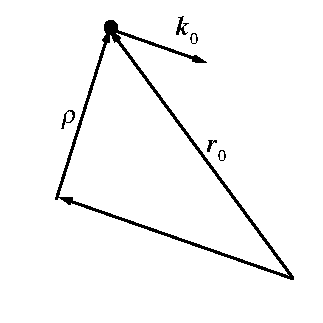
\includegraphics[clip,bb=17 15 170 170,width=5cm]{cond_in}
\caption{Initial condition after one of the relative energies have
converged}
\end{figure}

\begin{figure}[h]\label{f:cond-ini}
% \centering \resizebox{.5\linewidth}{!}{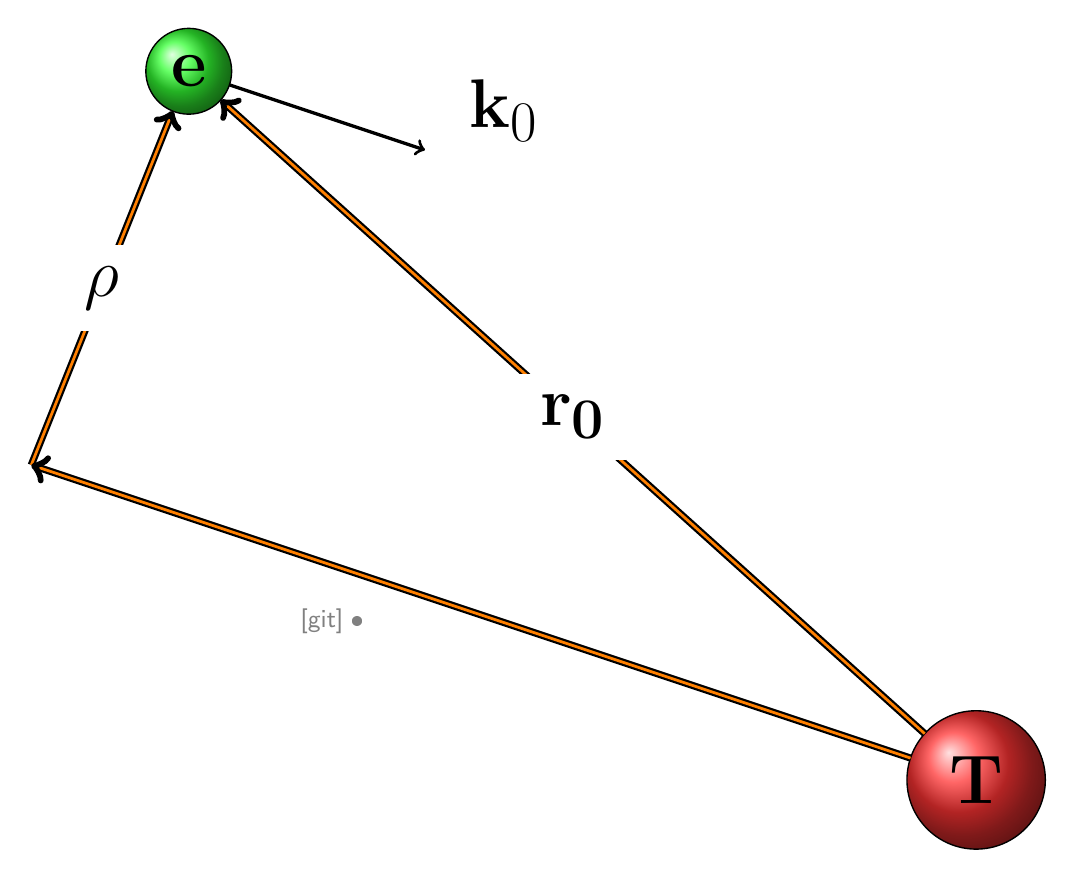
\begin{tikzpicture}
\GraphInit[vstyle = Shade]
\Huge
\tikzset{
  VertexStyle/.append style = { inner sep=5pt, minimum size=40pt ,
                                font = \bfseries},
  EdgeStyle/.append style = {->},
}

  \SetGraphUnit{5}
  \begin{scope}
    \tikzset{VertexStyle/.append style = {%
        shape= circle, shading= ball, ball color= red!80!white,%
        minimum size = 50pt,draw} } 
    \Vertex{T}
  \end{scope}

  \begin{scope}
    \tikzset{VertexStyle/.append style = {%
      shape= circle,shading= ball,ball color= green!80!white,%
      minimum size = 20pt,draw}
    }
    \Vertex[x=-10, y=9]{e}
  \end{scope}

  % velocidad   
  \draw [->,very thick] (e) -- (-7,8);
  \node at (-6,8.5) {$\vect{k}_{0}$};

  \Edge[label = $\bf{r}_{0}$](T)(e)
  \Edge[label = $\rho$](-12,4)(e)
  \Edge(T)(-12,4)


  % \draw [->, very thick] (6.8,0) arc [start angle=0, end angle=80, radius=1.1];
  % \node at (7.,1) {$\theta_{\ell}$};

  % \draw [<->, very thick] (0.,-1.2) arc [start angle=-90, end angle=0, radius=1.2];
  % \node at (1,-1.5) {$\theta_{\ell \ell'}$};
  % \Edge(X)(C)
  % \Edge(X)(D)
  % \Edge(X)(E)
  % \Edge(X)(A)
  % \Edge(X)(B)

\end{tikzpicture}


}
\caption{Initial condition after one of the relative energies have
converged}
\end{figure}
%\end{floatingfigure}


The impact parameter $\brho$ is given by the component of the distance,
perpendicular to the initial relative momentum $\vect{k}_{0}$,
\begin{equation}\label{Q:rho}
\brho = \hat{k}_{0} {\times} \left( \vect{r}_{0} {\times} \hat{k}_{0} \right)
\end{equation}

The final momentum will be given by
\begin{equation}\label{Q:finalmom}
\vect{p} = p_{E} \, \cos{\theta} \, \hat{k}_{0}+ p_{E}\, \sin{\theta}\,
\hat{\rho}
\end{equation}
%
where $\theta $ is the angle between $\vect{k}_{0}$ and $\vect{p}$. Then,
we only need to solve the ``\textit{off-shell}'' scattering problem
\cite{Fiol2000JPBp2847}.

%\begin{floatingfigure}[r]{8.2cm}
\begin{figure}[!htpb]
  \centering
 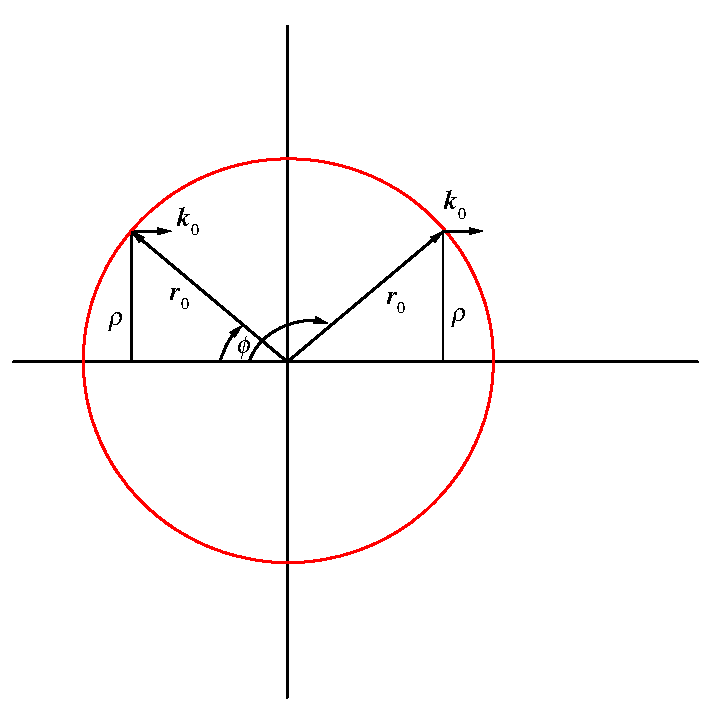
\includegraphics[width=7cm,bb=35 45 380 340,clip]{ctmc1}
  \caption{Problem equivalent to be solved.
  \label{f:ctmc1}}
\end{figure}
%\end{floatingfigure}


The solution of this problem is already known for Coulomb potential
$V(r) = Z/r$. In momentum space the trajectories of the particles are
circles of ratio $p_{R}$ and centered at $\vect{p}_{c}$ given by
\begin{eqnarray}\label{Q:circle-mom}
p_{R} &=& \frac{k_{0}}{2 \gamma} \, \frac{1}{\sin{\phi}} \nonumber \\
\\
\vect{p}_{c} &=& - \frac{k_{0}}{2 \gamma } \, \cot{\phi}\, \hat{\rho} +
\left( 1 + \frac{1}{2 \gamma} \right) \, \vect{k}_{0} \nonumber
\end{eqnarray}
where $\phi$ is the angle of the initial position ($\sin(\phi) =
\rho/r_{0}$) and $\displaystyle{\gamma = \frac{\left( k_{0}^{2}/2 m_{j}
\right)}{V(\vect{r}_{0})}}$.

% \begin{floatingfigure}[r]{8.2cm}
\begin{figure}%[!hptb]
  \centering
 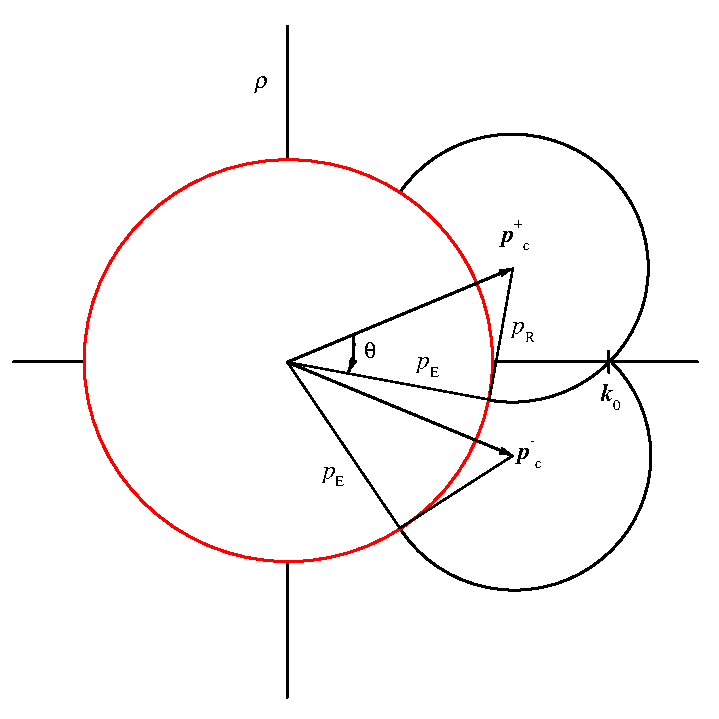
\includegraphics[width=7cm,clip,bb =35 35 380 380]{ctmc2}
  \caption{Solution of the problem in momentum space and definition of
  variables.
  \label{f:ctmc2}}
\end{figure}
%\end{floatingfigure}

While such a circle intersects the sphere of constant energy $p_{E}$ in
a rect angle (90$^{\circ}$), the angle of the final momentum relative to the
center $\vect{p}_{c}$ is given by

\begin{equation}\label{Q:angle}
\theta - \theta_{c} = {\rm sg}(Z) \, \arctan{\left( \frac{p_{R}}{p_{E}}
\right)} \ .
\end{equation}

The final momentum can be obtained replacing \ref{Q:angle} in
\ref{Q:finalmom}, with
\[
\theta_{c} = \arctan\left[(2 \gamma + 1) \, \rho / r_{0\, \|} \right]
\,.
\]

\section{Multiple-electron targets}

\subsection{Initialization of the target}
\label{S:Initi-targe}

First we set the electrons' momenta and coordinates fixing their
nucleus to the origin. This fixes their values to

\[
\vect{p}'_{j} = m_{j} \vect{p}_{T,j}/m_{T,j} \qquad \vect{r}'_{j} =
\vect{r}_{T,j}
\]

where $\vect{p}_{T}, \vect{r}_{T}$ are obtained in the center of mass
nucleus-electron (for both projectile target). The internal center of
mass velocity and position are
%
\[
M_{tot} \vect{v}_{cm} \equiv \sum_{j} \vect{p}'_{j}  \qquad M_{tot}
\vect{r}_{cm} \equiv \sum_{j} m_{j} \vect{r}'_{j}
\]

These two vectors have to be zero in the reference system attached to
the initial velocity of the whole fragment. At the same time the
relative velocities and distances between each electron and their
parent nucleus have to remain unchanged. Then constant velocities and
distances vectors must be subtracted to all momenta and positions such
that the new vectors verify simultaneously the following conditions
\begin{eqnarray*}
  0 &=& M_{N} \vect{r}_{N} + \sum_{j} m_{j} \vect{r}_{j} \\
  0 &=& M_{N} \vect{p}_{N} + \sum_{j} \vect{p}_{j} \\
\frac{\vect{p}_{j}}{m_{j}} - \frac{\vect{p}_{N}}{m_{N}} &=&
\frac{\vect{p}_{T,j}}{m_{T,j}}\, \vect{r}_{j}-\vect{r}_{N} = \vect{r}_{T}
\end{eqnarray*}

Finally, we have to translate these values to the initial position and
velocity of the fragment.

\section{Inclusion of tunneling}
\label{S:Inclu-tunne}

First we sketch the method used by Cohen \autocite{Cohen2001PRAp043412}. He proposed
to use the tunneling probability obtained in the semiclassical (JWKB)
approximation. Let's consider an atom immersed in an external
electromagnetic field. In the two-body center of mass system it is
equivalent to a particle of reduced mass $m_{\alpha}$ and charge
$Z_{\alpha}$ in a potential center $V_{\alpha}$. The tunneling
probability it is given by \cite{Galindo1990_QMvII}

\begin{equation}\label{Q:proba-tunne-JWKB}
\mathcal{P}_{\mathrm{tun}} \equiv T_{\mathrm{WKB}} = \exp{\left\{ -
\frac{2 \sqrt{(2 m_{\alpha})}}{\hbar} \int_{r_{1}}^{r_{2}} \left[
\mathcal{V}(\vect{r}) - \mathcal{V}(\vect{r}_{1})\right]^{1/2} d \vect{r}
\right\}} \, ,
\end{equation}
%
where $\vect{r}_{1}, \vect{r}_{2}$ are the turning points of the effective
potential $\mathcal{V}$ such that $\vect{r}_{2}$ is connected to the
continuum and $V(\vect{r}_{1})=V(\vect{r}_{2})$. It also is assumed that
the tunneling is instantaneous. The (reduced) particle is transported
from $\vect{r}_{1}$ to $\vect{r}_{2}$ while its velocity remains unchanged.

The first impression is that the potential in equation
\ref{Q:proba-tunne-JWKB} is given by
%
\begin{equation}\label{Q:effec-poten-JWKB}
\mathcal{V}(\vect{r}) = V(\vect{r}) + \frac{1}{2 m_{\alpha}}
\frac{L^{2}}{r^{2}} + Z_{\alpha} \vect{F}(t_{0})  \cdot \vect{r} \, ,
\end{equation}
%
where $L=\hbar (l+1/2) = \vect{k}_{\alpha} \cdot \vect{r}_{\alpha}$.
However we should check this.

The probability of tunneling must be evaluated every time the particle
reaches the position $\vect{r}_{1}$ or equivalently its momentum
(velocity) in the direction of the field vanishes ($\vect{k} \cdot
\vect{F}(t) =0$). Also the direction of the external field must be such
that it lowers the interaction potential in the direction that connects
$\vect{r}_{1}$ and $\vect{r}_{2}$ ($Z_{\alpha} \vect{F}(t_{0})  \cdot \vect{r}
< 0$).

\subsection{Hydrogen atom in an immersed field}
\label{S:Hydro-atom-immer-field}

%%% Local Variables: 
%%% mode: latex
%%% TeX-master: "main"
%%% End: 

\chapter{Time dependent approximation theory}
Here we will sketch some approaches to perturbation theory in time-dependent problems.

The quantum state is described by the wavefunction, solution of the time-dependent Schr\"{o}dinger equation (TDSE)
\begin{equation}\label{Q:td-tdse}
i \hbar \frac{\partial \Psi}{\partial t} = \hat{H}(t)  \Psi(\bm{r},t)= 
 \left[ \frac{\hat{\bm{p}}^{2}}{2 m} + V(\bm{r},t) \right]  \Psi(\bm{r},t) \,.
\end{equation}
with suitable initial conditions $\Psi(\bm{r},t_{0})= \Phi_{0}(\bm{r})$ 

\section{Evolution operator}
\label{S:evolution-operator}

The evolution operator is defined as the operator that takes the wavefunction to an initial time $t_{0}$ and returns the wavefunction to a time $t$
\begin{equation} \label{Q:td-defin-evolu-operat}
  \Psi(\bm{r},t)=  \hat{U}(t,t_{0}) \Psi(\bm{r},t_{0})
\end{equation}

This operator is hermitic, unitary $\left( \hat{U}^{\dag}(t,t_{0})= \hat{U}^{-1}(t,t_{0})= \hat{U}(t_{0},t) \right)$ and verifies an equation similar to the Schr\"{o}dinger equation
\begin{align}
  \label{Q:td-diffe-equat-opera-evolu}
  i\hbar \frac{\partial \hat{U}(t,t_{0})}{\partial t}&= \hat{H} \hat{U}(t,t_{0})\,, & \hat{U}(t_{0},t_{0})= \hat{1}
\end{align}
which is equivalent to the integral equation
\begin{equation}
  \label{Q:td-diffe-equat-opera-evolu-0}
  \hat{U}(t,t_{0}) = \hat{1} + \frac{1}{i\hbar} \int_{t_{0}}^{t} \hat{H}(t') \hat{U}(t',t_{0}) \, dt'
\end{equation}
Note that the two operator conmute ($[\hat{H}(t') , \hat{U}(t',t_{0})]=0$) such that this equation may be written as
\begin{equation}
  \label{Q:td-diffe-equat-opera-evolu-1}
  \hat{U}(t,t_{0}) = \hat{1} + \frac{1}{i\hbar} \int_{t_{0}}^{t}\hat{U}(t',t_{0})  \hat{H}(t') \, dt'
\end{equation}
\section{Interaction picture}
\label{S:interaction-picture}

The interaction picture is based in a separation of the system hamiltonian as a sum of two parts $\hat{H}= H^{0}_{i} + H'_{i}$.
where we know (or at lest will be able to solve) the problem for $H_{0}$. In this picture the states will only evolve due to the perturbation $H'_{i}$
\begin{equation}
  \label{Q:td-inter-pictu-state-evolu}
  |\psi_{i}(t) \rangle =  \hat{U}^{0 \dag}_{i}(t,t_{0}) \, |\psi(t) \rangle =  \hat{U}^{0 \dag}_{i}(t,t_{0}) \hat{U} (t,t_{0}) \, |\psi(t_{0}) \rangle 
\end{equation}
The evolution operator in this representation is given by
\begin{equation}
  \label{Q:td-repre-inter-opera-evol}
  \hat{U}_{i}(t,t_{0})=  \hat{U}^{0 \dag}_{i}(t,t_{0})\, \hat{U}(t,t_{0})
\end{equation}
%
where $ \hat{U}^{0 \dag}_{i}(t,t_{0})$ is the evolution operator that satisfies (\ref{Q:td-diffe-equat-opera-evolu}) for the Hamiltonian $H^{0}_{i}$. In particular, if $H^{0}_{i}$ does not depend on time it may be written as
\begin{equation*}
   \hat{U}^{0}_{i}(t,t_{0})= e^{-i H^{0}_{i} t/\hbar} \qquad \Rightarrow \qquad  \hat{U}^{0 \dag}_{i}(t,t_{0})= e^{i H^{0}_{i} t/\hbar} 
\end{equation*}
 Other operators in this representation are related to those in the Schr\"{o}dinger picture as
\begin{equation*}
  \hat{A}_{i}=  \hat{U}^{0 \dag}_{i}(t,t_{0})\,\hat{A} \,\hat{U}^{0}_{i}(t,t_{0})
\end{equation*}

The evolution operator in this representation verifies the integral equation
\begin{equation*}
  \hat{U}_{i}(t,t_{0}) = 1 + \frac{1}{i\hbar} \int_{t_{0}}^{t} V_{i}(t')\, \hat{U}_{i}(t',t_{0}) \, dt'
\end{equation*}
where $V_{i}$ is the interaction representation of the perturbation $H'_{i}$:
\begin{equation*}
  V_{i}= \hat{U}^{0 \dag}_{i}(t,t_{0})\, H'_{i} \,\hat{U}^{0}_{i}(t,t_{0}) \,.
\end{equation*}

Solving from eq. (\ref{Q:td-repre-inter-opera-evol}) and using the above integral equation we obtain
\begin{align}\label{Q:td-expan-oper-evol-1}
  \hat{U}(t,t_{0})&= \hat{U}^{0}_{i}(t,t_{0})\, \hat{U}_{i}(t,t_{0}) =  \hat{U}^{0}_{i}(t,t_{0})\,\left( 1 + \frac{1}{i\hbar} \int_{t_{0}}^{t} V_{i}(t')\, \hat{U}_{i}(t',t_{0}) \, dt' \right) \notag \\
&= \hat{U}^{0}_{i}(t,t_{0})\,\left( 1 + \frac{1}{i\hbar} \int_{t_{0}}^{t} V_{i}(t')\, \hat{U}^{0 \dag}_{i}(t',t_{0}) \, \hat{U}(t',t_{0}) \, dt' \right) \notag \\
 &= \hat{U}^{0}_{i}(t,t_{0}) + \frac{1}{i\hbar} \int_{t_{0}}^{t} \hat{U}^{0}_{i}(t,t_{0})\, V_{i}(t')\, \hat{U}^{0 \dag}_{i}(t',t_{0}) \, \hat{U}(t',t_{0}) \, dt' \notag \\
 &= \hat{U}^{0}_{i}(t,t_{0}) + \frac{1}{i\hbar} \int_{t_{0}}^{t} \hat{U}^{0}_{i}(t,t')\, \underbrace{\hat{U}^{0}_{i}(t',t_{0})\, V_{i}(t')\, \hat{U}^{0 \dag}_{i}(t',t_{0})}_{H'_{i}} \, \hat{U}(t',t_{0}) \, dt' \notag \\
 &= \hat{U}^{0}_{i}(t,t_{0}) + \frac{1}{i\hbar} \int_{t_{0}}^{t} \hat{U}^{0}_{i}(t,t')\, H'_{i} \, \hat{U}(t',t_{0}) \, dt' 
\end{align}
%
In the second line we have written the integrand in terms of the original Schr\"{o}dinger picture of the evolution operator. 

Now, we can iterate again using the integral equation and obtain a series of $n$ terms. We start noting that the above procedure is valid for \emph{all possible} separations of the hamiltonian. In the second iteration we may choose a different separation, yet another different in the third, and so on \dots
\begin{align*}
  \hat{U}(t,t_{0}) = \hat{U}^{0}_{i}(t,t_{0}) &+ \frac{1}{i\hbar} \int_{t_{0}}^{t}  dt_{i} \, \hat{U}^{0}_{i}(t,t_{i})\, H'_{i} \, \left( \hat{U}^{0}_{j}(t_{i},t_{0}) + \frac{1}{i\hbar} \int_{t_{0}}^{t_{i}} dt_{j} \, \hat{U}^{0}_{j}(t_{i},t_{j})\, H'_{j}(t_{j}) \, \hat{U}(t_{j},t_{0}) \right)  \\
 = \hat{U}^{0}_{i}(t,t_{0}) & + \frac{1}{i\hbar} \int_{t_{0}}^{t}  dt_{i} \, \hat{U}^{0}_{i}(t,t_{i})\, H'_{i}  \hat{U}^{0}_{j}(t_{i},t_{0}) + \\ 
 &+  \left( \frac{1}{i\hbar} \right)^{2} \int_{t_{0}}^{t} dt_{i} \, \int_{t_{0}}^{t_{i}}  dt_{j} \, \hat{U}^{0}_{i}(t,t_{i})\, H'_{i}(t_{i}) \, \hat{U}^{0}_{j}(t_{i},t_{j})\, H'_{j}(t_{j}) \, \hat{U}(t_{j},t_{0}) \\
 = \hat{U}^{0}_{0}(t,t_{0}) &+ \frac{1}{i\hbar} \int_{t_{0}}^{t}  dt' \, \hat{U}^{0}_{0}(t,t')\, H'_{1}(t')  \hat{U}^{0}_{1}(t',t_{0}) \\ 
&+  \frac{1}{(i\hbar)^{2}}  \int_{t_{0}}^{t} dt_{2} \, \int_{t_{0}}^{t_{2}} dt_{1} \, \hat{U}^{0}_{0}(t,t_{2})\, H'_{0}(t_{2}) \, \hat{U}^{0}_{1}(t_{2},t_{1})\, H'_{1}(t_{1}) \, \hat{U}(t_{1},t_{0})
\end{align*}
In order to illustrate the process we have iterated again using a separation of the hamiltonian $\hat{H}=H^{0}_{j} + H'_{j}$, where in principle $H'_{j} \neq H'_{i}$. Note that always $t_{1} < t_{2}$. If we keep repeating this procedure we get for the evolution operator
\begin{subequations}
  \begin{align}
    \label{Q:td-serie-evolu-opera}
    \hat{U}(t,t_{0}) =& \hat{U}^{0}_{0}(t,t_{0}) + \sum_{n=1}^{\infty} \frac{1}{(i \hbar)^{n}} \,\hat{U}^{(n)}(t,t_{0})  \\
    \hat{U}^{(n)}(t,t_{0}) =& \int_{t_{0}}^{t} dt_{n}\,\int_{t_{0}}^{t_{n}} dt_{n-1}\,\dots\,\int_{t_{0}}^{t_{2}} dt_{1}\, \hat{U}^{0}_{0}(t,t_{n})\, H'_{0}(t_{n}) \hat{U}^{0}_{1}(t_{n},t_{n-1}) \times \\
    &\times H'_{1}(t_{n-1}) \, \dots {\hat{U}^{0}_{n-1}(t_{2},t_{1})\, H'_{n-1}(t_{1})}
    \hat{U}^{0}_{n}(t_{1},t_{0}) \qquad \qquad \left( t_{1} < t_{2} < \dots t_{n-1} <
      t_{n} \right) \nonumber
  \end{align}
\end{subequations}
which reduces exactly to equation (9.47) of \citet{Tannor2007_ITQ} when the separation of the Hamiltonian $\hat{H}= H^{0}_{i} + H'_{i}$ is the same for all $i$.

\section{Transition probabilities and amplitudes}

\label{S:trans-prob-ampl}

The transition amplitude from an initial state $\phi_{i}$, prepared at time $t_{0}$ to a final state  $\phi_{f}(t)$ at a given time $t$ is given by the product 
%
\begin{equation} \label{Q:td-transi-ampli-t}
  t_{fi}(t)= \langle \phi_{f}(t) | \Psi(t) \rangle = \big\langle \phi_{f}(t) |\hat{U}(t,t_{0}) | \phi_{i}(t_{0}) \big\rangle 
\end{equation}
donde
%
\begin{subequations}
  \begin{align}
    &H_{0} \phi_{i(f)}(\bm{r},t)= E_{i(f)} \, \phi_{i(f)}(\bm{r},t)  & (\forall~ t )\\
    &\phi_{i(f)}(\bm{r},t)=   \phi_{i(f)}(\bm{r},t_{0})\, e^{-iE_{f(i)}t/\hbar}  &
  \end{align}
\end{subequations}
In particular, the transition amplitude is defined as
\begin{equation} \label{Q:td-defin-transi-ampli}
 T_{fi}= \lim_{\substack{t\to +\infty\\t_{0}\to -\infty}} t_{fi}(t)= \lim_{\substack{t\to +\infty\\t_{0}\to -\infty}} \big\langle \phi_{f}(t) |\hat{U}(t,t_{0}) | \phi_{i}(t_{0}) \big\rangle 
\end{equation}

Note that the transition amplitude may be also written as
\begin{align} \label{Q:td-transi-ampli-1}
 T_{fi}&= \lim_{\substack{t\to +\infty\\t_{0}\to -\infty}}  \big\langle \phi_{f}(t) |\hat{U}(t,t')\,\hat{U}(t',t_{0}) | \phi_{i}(t_{0}) \big\rangle  
=  \lim_{\substack{t\to +\infty\\t_{0}\to -\infty}} \big\langle \hat{U}(t',t) \phi_{f}(t) |\hat{U}(t',t_{0}) \phi_{i}(t_{0}) \big\rangle \nonumber\\
&= \big\langle \Psi^{-}_{f}(t') \left|\Psi^{+}_{i}(t') \right\rangle 
\end{align}
where we have defined the asymptotic states
\begin{equation}\label{Q:td-defin-asymp-state}
  \left| \Psi^{\pm}_{\alpha}(t) \right\rangle= \lim_{t_{0}\to \mp \infty} \hat{U}(t,t_{0})\, \phi_{\alpha}(t_{0})= \hat{U}(t,t_{0})\,\hat{U}_{\alpha}^{0\, \dag}(t,t_{0})\, \phi_{\alpha}(t) \qquad \qquad (\alpha= i,f)
\end{equation}

Two ``important'' cases correspond to evaluate the transition amplitude at infinite positive or negative (initial or final, respectively) times
\begin{subequations}
  \begin{align}
    \label{Q:T_fi-prior} T_{fi}^{-} &= \lim_{t \to -\infty}\big\langle \Psi^{-}_{f}(t) \big|\phi_{i}(t) \big\rangle  &&(\mathit{prior})\\
    \label{Q:T_fi-post} T_{fi}^{+} &= \lim_{t \to +\infty}\big\langle \phi_{f}(t) \big| \Psi^{+}_{i}(t) \big\rangle  &&(\mathit{post})
  \end{align}
\end{subequations}

An expresion that is usually employed is obtained by writing the above expresions as integrals of their derivatives. For instance for the \textit{prior} form of the transition matrix we obtain
\begin{subequations}
  \begin{align}\label{Q:td-T_fi-prior-work-expre-1}
    T_{fi}^{-} &= \lim_{t \to -\infty}\big\langle \Psi^{-}_{f}(t) \big|\phi_{i}(t) \big\rangle=  \lim_{t' \to -\infty} \int_{t_{1}}^{t'} \frac{d}{dt}\left( \big\langle \Psi^{-}_{f}(t) \big|\phi_{i}(t) \big\rangle \right) \, dt +  \big\langle \Psi^{-}_{f}(t_{1}) \big|\phi_{i}(t_{1}) \big\rangle  \\
    &= - \int_{-\infty}^{\infty} \frac{d}{dt}\left( \big\langle \Psi^{-}_{f}(t) \big|\phi_{i}(t) \big\rangle \right) \, dt +  \underbrace{\big\langle \Psi^{-}_{f}(t=\infty) \big|\phi_{i}(t=\infty)\big\rangle}_{\langle \phi_{f}|\phi_{i}\rangle=0} \notag \\
    &= - \int_{-\infty}^{\infty}  \left[ \left\langle \left. \frac{d \Psi^{-}_{f}(t) }{dt}  \right|\phi_{i}(t)\right\rangle  +  \left\langle \Psi^{-}_{f}(t) \left|\frac{d \phi_{i}(t)}{dt} \right. \right\rangle \right]  \, dt \notag \\
    &= \frac{1}{i \hbar} \int_{-\infty}^{\infty} \left[ \big\langle \Psi^{-}_{f}(t) \big|
      \hat{H} \big| \phi_{i}(t) \big\rangle - \big\langle \Psi^{-}_{f}(t) \big|
      \hat{H}_{i}^{0} \big| \phi_{i}(t) \big\rangle \right] \, dt =
    \frac{1}{i \hbar} \int_{-\infty}^{\infty} \big\langle \Psi^{-}_{f}(t) \big| \underbrace{\hat{H} - \hat{H}_{i}^{0}}_{V_{i}} \big| \phi_{i}(t) \big\rangle   \, dt \notag \\
\label{Q:td-T_fi-prior-work-expre-2}    &= \frac{1}{i \hbar} \int_{-\infty}^{\infty} \big\langle \Psi^{-}_{f}(t) \big| V_{i}(t) \big| \phi_{i}(t) \big\rangle \, dt
  \end{align}
\end{subequations}
where we have used equation (\ref{Q:td-defin-asymp-state}) and that both $|\Psi_{f}^{-}\rangle$ and $|\phi_{i}\rangle$ verify time-dependent Schr\"{o}dinger equations
\begin{subequations}
  \begin{align}
    & i \hbar \frac{d}{dt} |\Psi_{f}^{-}\rangle = \hat{H} |\Psi_{f}^{-}\rangle \qquad \Rightarrow & -i \hbar \frac{d \langle \Psi^{-}_{f}(t) | }{dt} = \langle \Psi^{-}_{f}(t) | \, \hat{H}\\
    & i \hbar \frac{d}{dt} |\phi_{i}\rangle = \hat{H} |\phi_{i}\rangle \,.
  \end{align}
\end{subequations}
%%% Local Variables: 
%%% mode: latex
%%% TeX-master: "main"
%%% End: 


\documentclass[english,oneside]{book}
  \RequirePackage{amssymb}[1995/01/01]

%\DeclareMathAlphabet{\bi}{OML}{cmm}{b}{it}
%\DeclareMathAlphabet{\bcal}{OMS}{cmsy}{b}{n}
%% MATH DEFINITIONS
%%
%% Define the roman letters to use in math mode (from iopart.cls)
%\newcommand{e}{\ensuremath{\mathrm{e}}}
%\newcommand{i}{\ensuremath{\mathrm{i}}}
%\newcommand{d}{\ensuremath{\mathrm{d}}}
%\newcommand{\Real}[1]{\ensuremath{\mathrm{Re}\left[ #1 \right]}}
%\newcommand{\Imag}[1]{\ensuremath{\mathrm{Im}\left[ #1 \right]}}
%
\begin{document}
\chapter{Coupled equations}
\section{Wavefunctions}

We assume at $t=-\infty$ the wavefunction is given by
\[
\Psi(\mathbf{r},\mathbf{R}) = \psi_{i,T} (\mathbf{r_{T}})
\]

At an arbitrary posterior time $t$ we expand the wavefunction as:
\begin{eqnarray}
\Psi(\mathbf{r},\mathbf{R},t) &=&
  \int c_{\mathbf{k},\mathbf{K}}(t) \psi_{\mathbf{k},\mathbf{K}}(\mathbf{r},\mathbf{R})\,
  e^{i E t}  d \mathbf{k} d \mathbf{K}  \\
&+& \sum_{j} a_{j}(t)) \Phi_{j,T}(\mathbf{r},\mathbf{R}) e^{i E t}
\nonumber \\
&+& \sum_{j}  b_{j}(t) \Phi_{j,P}(\mathbf{r},\mathbf{R}) e^{i E t}
\nonumber
\end{eqnarray}
%
where the states describe the continuum, target and projectile centered
states. The explicit expressions are:
\begin{eqnarray}\label{Q:CE-fi-T}
  \Phi_{j,T}(\mathbf{r},\mathbf{R}) &=& e^{i \mathbf{K}_{T} \cdot \mathbf{R}_{T}} \,
  \phi_{j,T}(\mathbf{r}_{T}) \,  \mathbb{E}(\mathbf{r}_{P},\mathbf{k}_{P})
  \\
  \Phi_{j,P}(\mathbf{r},\mathbf{R}) &=& e^{i \mathbf{K}_{P} \cdot \mathbf{R}_{P}} \,
  \phi_{j,P}(\mathbf{r}_{P}) \,  \mathbb{E}(\mathbf{r}_{T},\mathbf{k}_{T})
  \\
  \psi_{\mathbf{k},\mathbf{K}}(\mathbf{r},\mathbf{R}) &=& \frac{e^{i
(\mathbf{k}_j\cdot \mathbf{r}_j+\mathbf{K}_j\cdot \mathbf{R}_j)}}{(2
\pi)^3} \,
 D^{\pm}(\nu_T,\mathbf{k}_T,\mathbf{r}_T) \, D^{\pm}(\nu_P,\mathbf{k}_P,\mathbf{r}_P)
 \,D^{\pm}(\nu_N,\mathbf{k}_N,\mathbf{r}_N) \nonumber \\
\end{eqnarray}
Here $phi_{j,T(P)}$ are atomic functions of one center. In the case of
continuum states with Coulomb interactions the distortion factor is
given by \ref{Q:DFactCoul}
%
\[
D^{\pm}(\nu_j,\mathbf{k}_{j},\mathbf{r}_{j})= N^{\pm}(\nu_{j}) \,{_1F_1}\left(
\mp i \nu_{j};1; {\pm} i (k_{j} r_{j} \mp \mathbf{k}_{j}
\cdot\mathbf{r}_{j} ) \right) \, ,
\]
%
$N^{\pm}(\nu_j)= \Gamma(1 {\pm} i\nu_j) e^{-\pi \nu_j/2}$ and Sommerfeld's
parameter is defined by $\nu_j = m_j Z_j/ k_j$.

The energy can be written as $E=\frac{k_{T}^{2}}{2 m_{\alpha}}+
\frac{K_{T}^{2}}{2 m_{\alpha}} $


\section{Evolution of the wavefunction}
The wavefunction must obey the time-dependent Schr\"{o}dinger equation
\begin{equation}\label{Q:CE-tdse}
  \left( H - i\frac{\partial }{\partial t} \right)\Psi = 0\, , \qquad
  \qquad H=H_{0} + V_{T} + V_{P}+ V_{N} \,.
\end{equation}
%
We obtain
\begin{eqnarray}
i \int \dot{c}(\mathbf{k},\mathbf{K})(t)
\psi_{\mathbf{k},\mathbf{K}}(\mathbf{r},\mathbf{R}) d \mathbf{k} d
\mathbf{K}
  =
\int c_{\mathbf{k},\mathbf{K}}(t) \left( H - E \right)
\psi_{\mathbf{k},\mathbf{K}}(\mathbf{r},\mathbf{R})  d \mathbf{k} d \mathbf{K} \\
  \sum_{j}  a_{j}(t) \left( H - E \right) \Phi_{j,T}
  - i \dot{a}_{j}(t) \Phi_{j,T}
  \nonumber \\
+ \sum_{j} b_{j}(t) \left( H - E \right) \Phi_{j,P} -
  i \dot{b}_{j}(t) \Phi_{j,P}
 \nonumber
\end{eqnarray}

Then, we project on each base state. Using the continuum wavefunction
$\psi_{\mathbf{k}',\mathbf{K}'}$ we get
\[
\int  d \mathbf{k} d \mathbf{K}  \,  c_{\mathbf{k},\mathbf{K}}(t) \,
W^{c,c}_{\mathbf{k}',\mathbf{k}}  + \sum_{j} a_{j}
W^{c,T}_{\mathbf{k}',j} - i \dot{a}_{j} S^{c,T}_{\mathbf{k}',j} +
\sum_{l} b_{l} W^{c,P}_{\mathbf{k}',l} - i \dot{b}_{l}
S^{c,P}_{\mathbf{k}',l} = i \dot{c}_{\mathbf{k}',\mathbf{K}'}(t)
\]

Identically, when projecting on bound states,
\begin{eqnarray*}
\int  d \mathbf{k} d \mathbf{K}  \Big( c_{\mathbf{k},\mathbf{K}}(t) \,
W^{T,c}_{m,\mathbf{k}} - i \dot{c}_{\mathbf{k},\mathbf{K}}(t)
\,S^{T,c}_{m,\mathbf{k}} \Big) + \sum_{j} a_{j} W^{T,T}_{m,j} +
\sum_{l} b_{l} W^{T,P}_{m,l} - i \dot{b}_{l} S^{T,P}_{m,l} = i
\dot{a}_{m}\nonumber
  \\ %\\
\int  d \mathbf{k} d \mathbf{K}  \Big( c_{\mathbf{k},\mathbf{K}}(t) \,
W^{P,c}_{m,\mathbf{k}} - i \dot{c}_{\mathbf{k},\mathbf{K}}(t)
\,S^{P,c}_{m,\mathbf{k}} \Big) + \sum_{j} a_{j} W^{P,T}_{m,j} - i
\dot{a}_{j} S^{P,T}_{m,j} + \sum_{l} b_{l} W^{P,P}_{m,l} = i
\dot{b}_{m} \nonumber
\end{eqnarray*}
or, in matrix form:
%\begin{equation}\label{Q:CE-diff-equat}
%  \begin{array}{cccccc}
%     &  &  &  &  &  \\
%     &  &  &  &  &  \\
%     &  &  &  &  &  \\
%     &  &  &  &  &  \\
%     &  &  &  &  &  \\
%     &  &  &  &  & 
%  \end{array}
%\end{equation}


\noindent Where the coefficients are matrix elements given by
\begin{eqnarray}
W^{c,c} &=& \langle
\psi_{\mathbf{k}',\mathbf{K}'}|H-E|\psi_{\mathbf{k},\mathbf{K}} \rangle
 \\
W^{T,T} &=& \langle \Phi_{P,j'}|H-E|\Phi_{P,j'} \rangle
 \\
W^{P,P} &=& \langle \Phi_{P,j'}|H-E|\Phi_{P,j'} \rangle
 \\
W^{T,P} &=& \langle \Phi_{T,j'}|H-E|\Phi_{P,j'} \rangle
 \\
W^{P,c} &=& \langle \Phi_{P,j'}|H-E|\psi_{\mathbf{k},\mathbf{K}}
\rangle
 \\
W^{T,c} &=& \langle \Phi_{T,j}|H-E|\psi_{\mathbf{k},\mathbf{K}} \rangle
 \end{eqnarray}
%
and
%
\begin{eqnarray}
S^{T,P} &=& \langle \Phi_{T,j'}|\Phi_{P,j'} \rangle
 \\
S^{P,c} &=& \langle \Phi_{P,j'}|\psi_{\mathbf{k},\mathbf{K}} \rangle
 \\
S^{T,c} &=& \langle \Phi_{T,j}|\psi_{\mathbf{k},\mathbf{K}} \rangle
\end{eqnarray}

\subsection{Evaluation of coefficients}
\[
\mathbb{K}_{j} = \frac{\nabla_{\mathbf{r}_{j}}
D(\nu_{j};\mathbf{k}_{j},\mathbf{r}_{j})}{D(\nu_{j};\mathbf{k}_{j},\mathbf{r}_{j})}
\]
\end{document}

\chapter{Interactions with electromagnetic fields}
\label{C:Inter-with-elect-field}

We discuss the interaction of electromagnetic fields with matter. The
presentation follows closely that of references
\autocite{Bethe1997AC_IQM,Townsen2000_AMA}. Some parts are still missing and many need further elaboration.

\section{The Semiclassical approach}
\label{S:Semic-appro}
A widely used semiclassical treatment of the interaction of radiation with matter consists in a quantum-mechanical description of the particles and a classical description of the field \autocite{Bethe1997AC_IQM}.

\subsection{Classical Electromagnetic fields}

In a classical treatment, the electromagnetic field is obtained from the Maxwell equations
\begin{eqnarray}\label{Q:Maxwe-eq}
\nabla \cdot \bm{B} = 0 &,& \nabla {\times} \bm{E} +
  \frac{1}{c}\frac{\partial \bm{B}}{\partial t} = 0 \nonumber \\ \\
  \nabla  \cdot \bm{E} = 4 \pi \rho_{e} &,&
\nabla {\times} \bm{B} - \frac{1}{c} \frac{\partial \bm{E}}{\partial t} =
\frac{4 \pi}{c} \bm{J}_{\mathrm{e.m.}} \nonumber
\end{eqnarray}
Here, the charge density $\rho_{e}$ and electric current $J_{\mathrm{e.~m.}}$ are related by the continuity relation
\[
\frac{\partial \rho_{e}}{\partial t} + \nabla \cdot
\bm{J}_{\mathrm{e.m.}}= 0
\]

The first equation implies that the magnetic field can be expressed as the divergence of a certain vector potential $\bm{A}$. Similarly, the second one allows us to write the electric field in term of a scalar potential $\phi$
\[
\bm{B} = \nabla {\times} \bm{A} \quad , \qquad \bm{E} = - \left( \frac{1}{c} \frac{\partial \bm{A}}{\partial t} + \nabla \phi \right) .
\]
%
However, these equations do not fix the potential since every potential
that differs from these in the form
%
\begin{align*}
  \phi'(\bm{r},t) = \phi(\bm{r},t) - \frac{1}{c} \frac{\partial \xi(\bm{r},t)}{\partial t} \,,\\
  \bm{A}'(\bm{r},t) = \bm{A}(\bm{r},t) +  \nabla \xi(\bm{r},t)
\end{align*}
do not alter the magnetic and electric fields. The choice of the particular vector and scalar potential is called the ``gauge''.

The observable magnitudes are independent of the gauge chosen \autocite{Galindo1990_QMvI}. In many cases it is useful to choose the so-called Coulomb gauge in which
\begin{equation}\label{Q:Coul-Gaug}
  \nabla \bm{A} = 0 \, , \qquad \phi = 0 \,.
\end{equation}
%
Thus, the Maxwell equation result in
\begin{eqnarray}\label{Q:Maxwe-EZ-2}
\bm{B} &=& \nabla {\times} \bm{A} \label{Q:Maxwe-EZ-1}\\
\bm{E} &=& -\frac{1}{c} \frac{\partial \bm{A}}{\partial t}
\\
0 &=& \nabla^{2} \bm{A} - \frac{1}{c^{2}} \frac{\partial^{2}
\bm{A}}{\partial t^{2}} \label{Q:Maxwe-EZ-3}
\\
  0 &=& \nabla  \cdot \bm{A} \label{Q:Maxwe-EZ-4}
\end{eqnarray}

A specific solution of the wave equation \ref{Q:Maxwe-EZ-3} is
\begin{equation}\label{Q:Monoc-field}
\bm{A} = \bm{A}_{0}\, e^{i (\bm{k} \cdot \bm{r} - \omega t)} 
\end{equation}
%
with $\omega = k c$. Additionally, the Coulomb gauge (expressed by \ref{Q:Maxwe-EZ-4}) imposes the constraint $\bm{k} \cdot \bm{A}_{0} =
0$. Thus, the wave is transverse to the direction of propagation $\bm{k}$.

The most general solution of the Maxwell equation is a superposition of these monochromatic waves
\begin{equation}\label{Q:Gener-field}
\bm{A} = \frac{1}{\sqrt{V}}\sum_{\bm{k}} \left[ \sum_{\lambda} c_{\bm{k},\lambda} \, \hat{\epsilon}_{(\bm{k},\lambda)} e^{i (\bm{k} \cdot \bm{r} - \omega t)} + c^{*}_{\bm{k},\lambda} \, \hat{\epsilon}_{(\bm{k},\lambda)} e^{- i (\bm{k} \cdot \bm{r} - \omega t) } \right] 
\end{equation}
%
where the vector $\hat{\epsilon}$ is perpendicular to the propagation vector $\bm{k}$. $\lambda=1,2$ are the two components of $\hat{\epsilon}$ in this perpendicular plane such that $\bm{k} \cdot \hat{\epsilon}_{(\bm{k},\lambda)}=0$. $V$ is the volume of a box of finite dimensions $L_{x},L_{y},L_{z}$ used to normalize the field. The conjugate term in \ref{Q:Gener-field} is included in order to get a real potential vector.

From the Maxwell equation the electric and magnetic fields are
\begin{subequations}
  \begin{align}\label{Q:Elect-Magne-field}
    \bm{E} =& \frac{1}{\sqrt{V}}\sum_{\bm{k},\lambda}\frac{\omega}{c} \; \hat{\epsilon}_{(\bm{k},\lambda)} \left[ c_{\bm{k},\lambda} \,e^{i (\bm{k} \cdot \bm{r} - \omega t)} + c^{*}_{\bm{k},\lambda} \, e^{- i (\bm{k} \cdot \bm{r} - \omega t) } \right]
    \\
    \bm{B} =& \frac{1}{\sqrt{V}}\sum_{\bm{k},\lambda} \left(\bm{k} {\times} \hat{\epsilon}_{(\bm{k},\lambda)} \right) \left[ c_{\bm{k},\lambda} \, e^{i (\bm{k} \cdot \bm{r} - \omega t)} + c^{*}_{\bm{k},\lambda} \, e^{- i (\bm{k} \cdot \bm{r} - \omega t) } \right]
  \end{align}

\end{subequations}
Observe that in absence of charges and currents, the electromagnetic field energy is given by
\begin{equation}\label{Q:Energ-EM-free}
H_{\mathrm{E.M.}} = \frac{1}{8 \pi} \int d \bm{r} \left[ \left(
-\frac{1}{c} \frac{\partial \bm{A}}{\partial t}\right)^{2} + \left(
\nabla {\times} \bm{A} \right)^{2} \right] = \frac{1}{8 \pi} \int d \bm{r}
\left( E^{2} + B^{2} \right)
\end{equation}


\subsection{Linear, circular and elliptically polarizations}

\section{Hamiltonian of a particle in an E.M. field}

Lets consider a spinless particle of chage $Z$ immersed in an E. M.  field characterized by potentials $\phi, \bm{A}$ and an external potential $V(r)$. The classical hamiltonian is given by \textcite[][App.~E]{Townsen2000_AMA}
\begin{equation}\label{Q:Clas-Hamil-EM}
H = \frac{1}{2 m} \left( \bm{p} - \frac{Z \bm{A}}{c} \right)^{2} + Z \, \phi + V(r)
\end{equation}
%

Thus, the quantum mechanical time-dependent Schr\"{o}dinger equation (TDSE) is straightforwardly obtained
\begin{equation}\label{Q:QM-Hamil-EM}
i \hbar \frac{\partial \Phi}{\partial t} = \left[ \frac{1}{2 m} \left( - i \hbar \nabla - \frac{Z}{c}\bm{A} \right)^{2} + Z \phi + V(\bm{r})\right] \Phi \,.
\end{equation}


\subsection{Gauge Invariance and Gauge Choice}
\label{S:gauge-invar-choice}

This equation is invariant to gauge transformations. This means that for a given function $\xi(\bm{r},t)$ the above Schr\"{o}dinger equation does not change its form if we replace
\begin{subequations}
  \begin{align}
    \label{Q:ph-gauge-inv-phi}  \phi'(\bm{r},t) &= \phi(\bm{r},t) - \frac{1}{c} \frac{\partial \xi(\bm{r},t)}{\partial t} \,,\\
    \label{Q:ph-gauge-inv-A}  \bm{A}'(\bm{r},t) &= \bm{A}(\bm{r},t) +  \nabla \xi(\bm{r},t)\\
    \label{Q:ph-gauge-inv-wf} \Phi'(\bm{r},t) &= \Phi(\bm{r},t) \, e^{i\, Z/\hbar c\,
      \xi(\bm{r},t)}
  \end{align}
\end{subequations}
Two commonly used gauges are the velocity and length gauges. The Hamiltonian keeps its form (\ref{Q:Clas-Hamil-EM}) with the fields
\begin{subequations}
  \begin{align}
    &\text{velocity} & &\text{length} \notag \\
    \xi^{(v)}(\bm{r},t)&= (Z/2 m c) \int A^{2}(t') d t' & \xi^{(l)}(\bm{r},t)&= - \bm{A}(t) \cdot \bm{r} \\
    \bm{A}^{(v)}(\bm{r},t)&= \bm{A}(\bm{r},t) & \bm{A}^{(l)}(\bm{r},t) &= 0
    \\
    \phi^{(v)}(\bm{r},t)&= \phi(\bm{r},t) - \frac{Z}{2 m c^{2}} A^{2}(\bm{r},t) &
    \phi^{(l)}(\bm{r},t)&= \phi(\bm{r},t) + \frac{1}{c} \frac{\partial \bm{A}(t)}{\partial
      t} \cdot \bm{r}
  \end{align}
\end{subequations}

\subsection{Detailed calculations for velocity and length gauges}
\label{S:deta-calc-veloc-lengt-gauge}

Although is easy to introduce the above fields in the Schr\"{o}dinger equation and obtain the hamiltonian for the two gauges, we will show do the calculations.
In order to rewrite the Schr\"{o}dinger equation in terms of a (time dependent) force we write the wavefunction as:
\begin{equation}
  \label{Q:ph-volkov-1}
  \Psi(\bm{r},t) = e^{-i \alpha(\bm{r},t)} \, \Phi(\bm{r},t)
\end{equation}
and insert it in the Schr\"{o}dinger equation (\ref{Q:QM-Hamil-EM}). On the right hand side we have:
\begin{equation*}
\hat{H} \Phi(\bm{r},t) = \hat{H}  e^{i \alpha(\bm{r},t)} \, \Psi(\bm{r},t) = \left[ \frac{1}{2 m}
\left( - i \hbar \nabla - \frac{Z}{c}\bm{A} \right)^{2} + Z \phi + V(\bm{r})\right]  e^{i \alpha(\bm{r},t)} \, \Psi(\bm{r},t) 
\end{equation*}
%
First, let's investigate the left side of the Schr\"{o}dinger equation:
\begin{equation}
  \label{Q:ph-lhs-sch-eq}
    i \hbar \frac{\partial \Phi}{\partial t} = e^{i \alpha(\bm{r},t)} \, \left(   i \hbar \frac{\partial \Psi(\bm{r},t)}{\partial t} - \hbar \frac{d \alpha}{d t} \Psi(\bm{r},t) \right) 
\end{equation}

The operation of the ``momentum'' on this wavefunction is:
\begin{align}\label{Q:ph-momentum-action}
  \left( - i \hbar \nabla - \frac{Z}{c}\bm{A} \right)\, e^{i \alpha(\bm{r},t)} \, \Psi(\bm{r},t)&= e^{i \alpha(\bm{r},t)} \,  \left\{  - i \hbar  \left[ i (\nabla \alpha) \Psi(\bm{r},t) +  \nabla \Psi(\bm{r},t) \right] - \frac{Z}{c}\bm{A} \Psi(\bm{r},t)  \right\} \nonumber \\
  &= \left[ \hbar (\nabla \alpha) - \frac{Z}{c}\bm{A} \right]\,e^{i \alpha(\bm{r},t)}
  \Psi(\bm{r},t) - i \hbar \, e^{i \alpha(\bm{r},t)} \, \nabla \Psi(\bm{r},t)
\end{align}
 %
The choice of the exponent $\alpha$ is what it is called \textbf{gauge} choice.



\subsubsection{Velocity Gauge}
\label{S:velocity-gauge}
The \textbf{velocity gauge} is chosen such that the term quadratic in the vector field, $A^{2}$ is removed from the Schr\"{o}dinger equation. It is easy to show that this is accomplished by choosing
\begin{equation}
\label{Q:ph-alpha-vel} \alpha(\bm{r},t)\equiv \alpha_{(v)}= \frac{-Z^{2}}{2 m \hbar c^{2}}  \,\int  A^{2}(t') \, dt' \,.
\end{equation}

With this choice we have:
\begin{align}
  \label{Q:ph-alpha-vel-deriv-t}
  \frac{d \alpha}{d t} &= \frac{-Z^{2}}{2 m \hbar c^{2}} \, A^{2}(t)& \text{and} &&  \nabla \alpha &= 0
\end{align}
and the momentum acting on the wavefunction may be written from (\ref{Q:ph-momentum-action}) as

\begin{align*}
  \left( - i \hbar \nabla - \frac{Z}{c}\bm{A} \right)^{2} \, e^{i \alpha(\bm{r},t)} \, \Psi(\bm{r},t) &= \left( - i \hbar \nabla - \frac{Z}{c}\bm{A} \right)\left[ - \frac{Z}{c}\bm{A} \,e^{i \alpha(\bm{r},t)} \Psi(\bm{r},t) - i \hbar \, e^{i \alpha(\bm{r},t)} \, \nabla \Psi(\bm{r},t) \right] \\
&=  e^{i \alpha(\bm{r},t)} \,\left( \frac{Z^{2}}{c^{2}} A^{2} + 2 i \hbar \frac{Z}{c} \bm{A} \cdot \nabla \Psi - \hbar^{2} \nabla^{2} \Psi  \right)
\end{align*}
%
while replacing (\ref{Q:ph-lhs-sch-eq}) in the L.H.S gives
\begin{equation*}
  i \hbar \frac{\partial \Phi}{\partial t} = e^{i \alpha(\bm{r},t)} \, \left( i \hbar \frac{\partial \Psi(\bm{r},t)}{\partial t} + \frac{Z^{2}}{2 m  c^{2}} \, A^{2}(t)  \Psi(\bm{r},t) \right) \,.
\end{equation*}

Replacing these expresions in the Schr\"{o}dinger equations we obtain
\begin{equation}
  \label{Q:ph-schrod-gauge-vel}
    i \hbar \frac{\partial \Psi(\bm{r},t)}{\partial t} = \left[ \frac{\hat{\bm{p}}^{2}}{2m} +  Z \phi +  V(\bm{r}) + \frac{i \hbar Z}{m c} \bm{A}(t) \cdot \nabla \right]  \Psi(\bm{r},t)  \,.
\end{equation}


\subsubsection{Length Gauge}
\label{S:length-gauge}
We can make vanish the first term if we choose $\alpha$ such that $\nabla \alpha = (Z/\hbar c) \bm{A}$. For a simple potential vector that does not depend on $\bm{r}$ this gives
\begin{equation}
\label{Q:ph-alpha-len}  \alpha(\bm{r},t) \equiv \alpha_{(l)}= \frac{Z}{\hbar c}\, \bm{A}(t) \cdot \bm{r}
\end{equation}
%
With this choice we obtain
\begin{eqnarray*}
  \left( - i \hbar \nabla - \frac{Z}{c}\bm{A} \right)^{2}\, e^{i \alpha(\bm{r},t)} \, \Psi(\bm{r},t)&=& -i \hbar \left( - i \hbar \nabla - \frac{Z}{c}\bm{A} \right) e^{i \alpha(\bm{r},t)} \, \left( \nabla \Psi(\bm{r},t) \right) \\ 
&=&  e^{i \alpha(\bm{r},t)} \, (-i \hbar)^{2}  \nabla^{2} \Psi(\bm{r},t) =  e^{i \alpha(\bm{r},t)} \, \hat{\bm{p}}^{2} \Psi(\bm{r},t)
\end{eqnarray*}
and the right hand side of the Hamltonian (\ref{Q:QM-Hamil-EM}) reads
\begin{equation}
  \label{Q:ph-Hamilt-EM-1}
  \hat{H} \Phi(\bm{r},t)=  e^{i \alpha(\bm{r},t)} \,\left[ \frac{\hat{\bm{p}}^{2}}{2m} +  Z \phi + V(\bm{r})\right] \Psi(\bm{r},t)
\end{equation}

On the left hand side we obtain
\begin{equation*}
  i \hbar \frac{\partial \Phi}{\partial t} = i \hbar \frac{\partial \left( e^{i \alpha(\bm{r},t)} \, \Psi(\bm{r},t) \right)}{\partial t} = \hbar \,  e^{i \alpha(\bm{r},t)}\, \left(  i \frac{\partial \Psi(\bm{r},t)}{\partial t} - \frac{d \alpha}{d t} \Psi(\bm{r},t) \right) 
\end{equation*}

Now, combining this equation with eqs.~(\ref{Q:ph-alpha-len},~\ref{Q:ph-Hamilt-EM-1}) we obtain
\begin{equation}
  \label{Q:ph-hamil-EM-force}
  i \hbar \frac{\partial \Psi(\bm{r},t)}{\partial t} = \left[ \frac{\hat{\bm{p}}^{2}}{2m} +  Z \phi +  V(\bm{r}) + \bm{F}(t) \cdot \bm{r} \right]  \Psi(\bm{r},t) 
\end{equation}
where
\begin{equation*}
  \bm{F}(t) \equiv - Z \bm{E}(t) = -Z\, \left(- \frac{1}{c} \frac{\partial \bm{A}(t)}{\partial t} \right)
\end{equation*}


\subsection{Free particle immersed in a E.M. field: length gauge}
\label{S:Free-parti-immer-E.M.-field}

We first start studying the effect of a radiation field in a free particle. As expressed by \ref{Q:QM-Hamil-EM} the hamiltonian of a quantum system is obtained by replacing $\hat{\bm{p}} \to \hat{\bm{p}}-( Z / c ) \bm{A}$. As shown in the previous section, in the length gauge this Hamiltonian may in turn be converted to
\begin{equation}\label{Q:Schro-eq-free-parti}
  \hat{H} = \frac{\hat{\bm{p}}^{2}}{2m} + \bm{F}(t) \cdot \bm{r}  \quad  , \qquad \qquad  \bm{F}(t)= Z\, \frac{1}{c} \frac{\partial \bm{A}(t)}{\partial t} 
\end{equation}
%
A solution for the Time Dependent Schr\"{o}dinger Equation (TDSE) can be proposed as
\[
\psi(\bm{r},t) = \exp{\left\{ (i/\hbar)\left(  \bm{K}(t) \cdot \bm{r} - \int_{t_{0}}^{t}\frac{\bm{K}(t')^{2}}{2m} dt' \right) \right\}}
\]
where $\bm{K}(t)$ is still a function to determine. Applying the hamiltonian to this wavefunction we obtain
%
 \begin{eqnarray*}
  i \hbar \frac{\partial \psi}{\partial t} &=& \left(  \frac{\hat{\bm{p}}^{2}}{2m} + \bm{F}(t) \cdot \bm{r}  \right) \psi(\bm{r},t) \\
\left[ \frac{K(t)^{2}}{2m} - \frac{\partial \bm{K}(t)}{\partial t} \cdot \bm{r} \right] \psi(\bm{r},t)  &=& \left[ \frac{K(t)^{2}}{2m}  + \bm{F}(t) \cdot \bm{r} \right] \psi(\bm{r},t) 
\end{eqnarray*}
Thus, the unknown function must verify
\begin{equation}
\label{Q:ph-volkov-K}  \frac{\partial \bm{K}(t)}{\partial t} = - \bm{F}(t)= Z\, \frac{1}{c} \frac{\partial \bm{A}(t)}{\partial t}  \qquad \Rightarrow \qquad  \bm{K}(t)= - \frac{Z}{c} \bm{A}(t) + \mathrm{cte} \, .
\end{equation}
%
The constant must be determined from boundary (initial or final) conditions. For instance if we require that for earlier times the field is not active $A(-\infty)=$0, the state must be a plane wave with momentum $\bm{k}$, giving the so-called Volkov states
\begin{equation} \label{Q:ph-volkov-state}
\psi(\bm{r},t) = \exp{\left\{ (i/\hbar)\left[\left( \bm{k} - \frac{Z}{c} \bm{A}(t) \right)\cdot \bm{r} - \frac{1}{2m} \,\int_{t_{0}}^{t} \left( \bm{k} - \frac{Z}{c} \bm{A}(t) \right)^{2} dt' \right] \right\}}  \,.
\end{equation}

\subsection{Free particle in the velocity gauge}
\label{S:free-part-veloc}

In the velocity gauge the Hamiltonian of a ``free-particle'' is
\begin{equation*}
  \hat{H} = \frac{\hat{\bm{p}}^{2}}{2m} + i \frac{Z \hbar}{m c}\, \bm{A}(t) \cdot \nabla
\end{equation*}
By using that the solutions in different gauges are related we can obtain the solution to this equation
\begin{align}
  \psi^{(v)}(\bm{r},t) &= e^{i (\alpha_{(l)} - \alpha_{(v)})} \psi^{(l)} = \exp{\left[i \frac{Z}{\hbar c} \bm{A} \cdot \bm{r} + i \frac{Z^{2}}{2 m \hbar c^{2}}  \right]} \times \psi^{(l)}(\bm{r},t) \\
&= e^{i (\bm{k}\cdot \bm{r} - E_{k}t)/\hbar} \, \exp{\left[ i \frac{Z}{\hbar m c} \bm{k} \cdot \int_{t_{0}}^{t} \bm{A}(t') \, dt' \right]}
\end{align}
%
It is straightforward to verify that this wavefunction is solution of the time-dependent Schr\"{o}dinger equation.

\section{Interaction of photons with atoms}

After having obtained an expression for the external field $\bm{A}$, we consider now its effect on a quantum system. The hamiltonian for the system can be decomposed in the sum of three terms: the atomic $H_{At}$, the electromagnetic $H_{EM}$ (given by \ref{Q:Energ-EM-free}) and a final term describing the interaction between these two systems $H_{I}$. Expanding the kinetic energy term in eq.~\ref{Q:QM-Hamil-EM} we obtain, for the interaction term,
%
\begin{eqnarray}\label{Q:H_int-EM}
H_{I} = \frac{i \hbar Z}{m c}\, \bm{A} \cdot \nabla +
\frac{Z^{2}}{c^{2}} \, A^{2}
\end{eqnarray}
%
where we have used that in the Coulomb gauge $\nabla \bm{A}=0$.

Let's consider a system (for instance an atom) initially in a state $n_{i}$. The probability of finding it in a state $n_{f}$ at a posterior time $t$ is, at first order,
\begin{equation}\label{Q:first-order-trans-ampli}
a_{fi}^{(1)}(t) = \frac{1}{i \hbar} \int_{0}^{t} \langle
f|H_{I}(t')| i \rangle \; e^{i \omega_{fi} t'} d t'
\end{equation}
where $\omega_{fi} = (E_{f}-E_{i})/\hbar$, and the states $| i\rangle, | f\rangle$ are eigenvectors of the isolated hamiltonian $H_{0} = H_{At} + H_{EM}$. Using expression \ref{Q:Gener-field} the transition probability can be written for each monochromatic wave as
\begin{equation}\label{Q:first-order-trans-ampli-1}
a_{fi}^{(1)}(t) = - \frac{T'_{fi}}{\hbar} \frac{e^{i (\omega_{fi}-\omega)t} -1}{\omega_{fi} - \omega} \, e^{i \theta}
- \frac{T''_{fi}}{\hbar} \frac{e^{i (\omega_{fi} + \omega)t} -1}{\omega_{fi} + \omega} \, e^{- i \theta} \,,
\end{equation}
%
where
\begin{eqnarray} \label{Q:Tif-EM-1}
T'_{fi} &=& \frac{i Z \hbar}{m c} |c_{\bm{k},\lambda}| \int u^{*}_{f} \; e^{i \bm{k} \cdot \bm{r}} \;
\hat{\epsilon}_{(\bm{k},\lambda)}  \cdot \nabla u_{i} \; d \tau
\\
T''_{fi} &=& \frac{i Z \hbar}{m c} |c_{\bm{k},\lambda}| \int u^{*}_{f} \; e^{- i \bm{k} \cdot \bm{r}} \;
\hat{\epsilon}_{(\bm{k},\lambda)}^{*} \cdot \nabla u_{i} \; d \tau
\end{eqnarray}
where, for simplicity we have included the phase of $c_{k,\lambda}$ to the polarization vectors $\hat{\epsilon}_{(\bm{k},\lambda)}$.

Each of the two terms in expression \ref{Q:first-order-trans-ampli} has a maximum when $\omega_{fi} = \omega $, indicating that the change in the energy of the quantum system is quantized
%
\[ E_{f} = E_{i} \pm \hbar \omega \,. \]
%
Observe that the quantization of the field is not necessary because the atomic system itself can only exchange quantas of energy. The two terms in equation \ref{Q:Tif-EM-1} correspond to absorbtion ($T'$) and induced emission ($T''$) of one photon from the radiation field.

Since the density of states in a box is given by
\begin{equation}\label{Q:Densi-state}
\rho ( k_{f}) = \frac{V}{(2 \pi \hbar)^{3}}\frac{k_{f}^{2 d
k_{f}}}{V} d \Omega_{f}
\end{equation}
%
the rate of transitions from initial state $i$ to a final $f$ by absorption of radiation is
\begin{equation}\label{Q:Trans-Rate}
W = \frac{Z^{2}}{(2\, \pi \, \hbar \, c)^{2}} \frac{k_{f}}{m}
|c_{\bm{k}, \lambda}|^{2}
  \left|\int
u_{f}^{*} e^{i \bm{k} \cdot \bm{r}} \, \hat{\epsilon} \cdot
\nabla u_{i} d \tau \right|^{2} \, V \,d \Omega_{f}
\end{equation}

In the case of non-monochromatic radiation we must sum over all the terms expressed in \ref{Q:Gener-field}.

\section{Quantization of the radiation field}


\section{Multipole expansion}
\label{S:Multi-expan}

We expand the exponential in the computation of $T'$ and keep only the few first terms leading to a non-vanishing integral. The limit of validity and justification of this approximation can be obtained by estimating the values of $r$ at which the integrand in \ref{Q:first-order-trans-ampli} contributes significantly.  
%
Because the initial wavefunction $u_{i}$ corresponds to an bound atomic state, the typical values of $r$ are of the order of 1~a.~u. Since $k = 2 \pi/\lambda$, $k\,r = 2 \pi r/ \lambda$ and while the order of magnitude of the wavelength of radiation available in laboratories is at about a hundred nanometers (100~nm = 1000~\AA $\approx$ 2.~10$^{4}$~a.~u.), typical values for the argument in the exponential are $k\,r\approx 10^{-3}$. For these small values, the exponential can be expanded in a Taylor series
\[
e^{-i \bm{k} \cdot \bm{r}} = 1 - i \bm{k} \cdot \bm{r} + \frac{\left( i \bm{k} \cdot \bm{r}\right)^{2}}{2!} - \frac{\left(
i \bm{k} \cdot \bm{r}\right)^{3}}{3!} + \dots
\]

\subsection{Electric dipole approximation}

The electrical dipole approximation is obtained by retaining the first (constant) term
\[ e^{-i \bm{k} \cdot \bm{r}} \to 1 \, . \]
%
Thus, the integral in equations \ref{Q:Trans-Rate} can be written as
%
\[
I_{fi} = \hat{\epsilon}  \cdot \, \int u^{*}_{f}(\bm{r}) \, \nabla u_{i}(\bm{r}) d \bm{r}
\]
%
which, we will inmediately see, is equivalent to the action of a perturbation potential depending on an electric dipole
\begin{equation}\label{Q:dipol-approx-pertur-1}
  H_{I} = - \vec{\bmu}_{e}  \cdot \breve{\bm{E}} \, .
\end{equation}

In order to derive this result, lets remember that the gradient is
proportional to the momentum operator $\breve{\bm{p}} \equiv {(i /
\hbar)} \nabla $ and its commutator with the position operator is
simply $ [ \breve{\bm{r}}, \breve{\bm{p}} ] = i \hbar $. Then, the
commutator of $\breve{\bm{r}}$ and the hamiltonian $\breve{H} =
\breve{\bm{p}}^{2}/2 m + V(\breve{\bm{r}})$ is simply
%
\[
[\breve{H},\breve{\bm{r}}] = \frac{1}{2 m} \left[ \breve{\bm{p}}^{2} ,
\breve{\bm{r}} \right] = \frac{\breve{\bm{p}}}{m} [ \breve{\bm{p}} ,
\breve{\bm{r}} ] = - \frac{i \hbar}{m} \, \breve{\bm{p}} \,.
\]

The above integral can be written
\begin{eqnarray*}
I_{fi} &=& \frac{\hbar }{i} \hat{\epsilon}  \cdot \langle u_{f} |
\breve{\bm{p}}| u_{i}\rangle \\
&=& - \frac{m}{i \hbar} \frac{\hbar }{i} \hat{\epsilon} \cdot
\langle
u_{f} | [\breve{H},\breve{\bm{r}}] | u_{i}\rangle \\
&=& m\, \hbar \, \frac{\left(E_{f} - E_{i}\right)}{\hbar}
\hat{\epsilon}
\cdot \langle u_{f} |\bm{r} | u_{i}\rangle \\
\end{eqnarray*}
%
This last result corresponds to make the replacement $H_{I} \to q
\bm{r} \cdot \bm{E} \equiv - \vec{\bmu}_{e} \cdot \bm{E}$, giving a
transition rate proportional to the vector product of the polarization
and the matrix element
\[
\hat{\epsilon} \cdot \langle u_{f}|\bm{r}| u_{i}\rangle
\]

\subsubsection{Classical interpretation}

To do, see \citet{Bethe1997AC_IQM}.

\subsubsection{Line breadth of atoms}

Example for 2p state of hydrogen \autocite[see][]{Bethe1997AC_IQM,Townsen2000_AMA}


\subsection{Magnetic dipole and Electric Quadrupole Transitions}



\subsection{Antihydrogen formation}

%%% Local Variables: 
%%% mode: latex
%%% TeX-master: "main"
%%% End: 

\chapter{Laser-assisted collisions}

In this chapter we study how atomic systems are affected by laser pulses. Later, we study also how collisions between particles (ion-atom, electron-atom, etc) can be modified by the presence of an external field.

\section{Interaction of photons with atoms and molecules}

\subsection{Photoionization}
\label{S:photoionization}


\subsection{Atomic stabilization}
\label{S:atomic-stabilization}

Multiple-electron atoms can be stabilized by a laser \cite{Gavrila2002JPBpR147}


\section{Atomic ionization by a laser pulse}
\label{S:atomic-ionization}
Let's consider the ionization of an hydrogen atom by interaction with a laser pulse. We will consider the pulse as the force produced by an electric field derived from a vector potential $\bm{A}(t)$, that for the dimensions involved in the dynamics of atoms may be considered as uniform. As previously derived, the Hamiltonian for this system may be written as a time-dependent external force (\ref{Q:ph-hamil-EM-force}). We will consider a finite electric pulse of the form
\begin{equation} \label{Q:electric-field-Ft-0}
\bm{F}(t)= F_{0}\, \sin{(\omega (t-t_{0}))}\; \sin^{2}{(\pi\,t/\tau)} 
\end{equation}
for $0 < t < \tau $ and that vanishes at all other times. This field may be rewritten as:
\begin{equation} \label{Q:electric-field-Ft}
\bm{F}(t)= \frac{1}{4}\left[2\, \sin \left(\omega\, (t-t_{0})\right) - {\sin \left(\omega \, (t-t_{0}) +{{2\,\pi\,t}\over{\tau}}\right) - \sin \left(\omega\, (t-t_{0}) - \frac{2\,\pi\,t}{\tau} \right)} 
 \right]
\end{equation}

For a Hamiltonian that may be splitted into two parts $H=H^{0}+V$, the transition amplitude for a time-dependent problem may be written in its prior form as (\ref{Q:td-T_fi-prior-work-expre-1})
\begin{equation*}
  T_{fi}^{-}= \frac{1}{i \hbar} \int_{-\infty}^{\infty} \big\langle \Psi^{-}_{f}(t) \big| V_{i}(t) \big| \phi_{i}(t) \big\rangle   \, dt \,.
\end{equation*}

\subsection{Coulomb-Volkov approximation (Length gauge)}
\label{S:coul-volk-appr}

We consider the potential due to the laser as the perturbation ($V_{i}(t)= \bm{F}(t)\cdot \bm{r}$) wich vanishes outside the time-interval $\Delta T= (0, \tau)$ we can write the transition matrix as
\begin{equation*}
  T_{fi}^{-}= \frac{1}{i \hbar} \int_{0}^{\tau} \big\langle \Psi^{-}_{f}(t) \big| \bm{F}(t)\cdot \bm{r} \big| \phi_{i}(t) \big\rangle   \, dt \,.
\end{equation*}

Notice that if we write the final state wavefunction $|\Psi_{f}^{-}\rangle$ back using expression \eqref{Q:T_fi-post} we obtain 
the form used in eq.~30 of \citet{Milosev2006JPBpR203}:
\begin{equation}\label{Q:tif-milos-form}
T_{if}^{-}  = \frac{1}{i \hbar} \lim_{t \to \infty} \int_{0}^{\tau} \big\langle \phi_{f}(t) \big| U(t',t)  \bm{F}(t')\cdot \bm{r} \big| \phi_{i}(t') \big\rangle \, dt'
\end{equation}

The Coulomb-Volkov approximation consists in replacing the \textbf{exact wavefunction} $|\Psi^{-}_{f}(\bm{r},t)\rangle$ by a product of wavefunctions corresponding to the solution of two separated problems: the one of an isolated atom and the one of an electron in the external field. The plane wave part must be corrected to get the right boundary conditions (for $|\bm{r}|\to \infty$ and $|t| > \Delta T$).

The factor corresponding to the atomic interaction is the same that in atomic collisions, as used in CDW theories (or FBA theories for the target wavefunction).

The factor including the E.M field is obtained from \eqref{Q:ph-volkov-state} taking into account that the constant in \eqref{Q:ph-volkov-K} must be chosen as to describe a plane wave for $t=+\infty$. We consider that before the pulse starts $\bm{A}(t)=0$ ($t<0$). At all times the vector potential is given by
\begin{equation*}
  \bm{A}(t)= - c \int_{-\infty}^{t} \bm{E}(t') dt' = - c \int_{0}^{t} \bm{E}(t') dt' 
\end{equation*}
Notice that if the electric field $\bm{E}$ is symmetric the vector potential $\bm{A}(t)=0$ for $t>\tau$ but in general it is constant $\bm{A}(t)=A(\tau)\ne 0\,$.

Except by an arbitrary constant phase the wavefunction for $t=\tau$ is given by
\begin{equation*}
  \Psi(\bm{r},\tau) = e^{i \bm{k}\cdot\bm{r}/\hbar} e^{-i E_{k} \tau/\hbar} e^{i \varphi} \equiv e^{i \bm{k}\cdot\bm{r}/\hbar} 
\end{equation*}
which corresponds to a free particle with momentum $\bm{k}$ and must be compared with \eqref{Q:ph-volkov-state} with $ \bm{k}= \bm{p} - (Z/c)\,\bm{A}(\tau)$. 

For $t<\tau$ we have
\begin{align*}
  \Psi (\bm{r},t) &= e^{i \left[ \bm{p} - (Z/c)\bm{A}(t)\right]\cdot\bm{r}}\, \exp{\left[ \frac{-i}{2 m \hbar} \int_{\tau}^{t} \left( \bm{p} - \frac{Z}{c} \bm{A}(t') dt' \right)^{2}\right]} \\
\intertext{or in terms of the asymptotic momentum}
  \Psi (\bm{r},t) &= e^{i \left[\bm{k} - (Z/c)\bm{A}^{-}(t)\right]\cdot\bm{r}}\, \exp{\left[ \frac{-i}{2 m \hbar} \int_{\tau}^{t} \left( \bm{k} - \frac{Z}{c} \bm{A}^{-}(t') dt' \right)^{2}\right]}\ , &   \bm{A}^{-}(t)&=  \bm{A}(t) - \bm{A}(\tau) \,.
\end{align*}

Summarizing we can approximate the wavefunction $\left|\Psi_{f}^{(-)}\right\rangle \approx \left|\chi_{f}^{(-)} \right\rangle$ where
\begin{align}
  \label{Q:defin-coul-volk-state}
  \chi^{-}_{f}(\bm{r}, \bm{k}, t) &= \frac{e^{i \bm{k}\cdot \bm{r}/\hbar}}{2 \pi \hbar}\, D^{-}_{\nu}(\bm{k}, \bm{r}) \, D^{-}_{\bm{A}}(\bm{k}, \bm{r}, t) \, e^{-i E_{f} (t- \tau)/\hbar} \qquad \qquad \left(E_{f}=k^{2}/2m \right)\\
 D^{\pm}_{C}(\bm{k}, \bm{r}) &= \frac{e^{i \bm{k}\cdot \bm{r}/\hbar}}{2 \pi \hbar}\,\phi^{\pm}_{f}(\bm{r}) && (\text{see eq}.~\ref{Q:DFact})\nonumber \\
\label{Q:def-Da-CV} D^{\pm}_{\bm{A}(t)}(\bm{k}, \bm{r}, t) &= e^{i \bm{A}^{\pm}(t) \cdot \bm{r}/\hbar}\, \exp{\left[ \frac{-(i/\hbar)}{m}\, \bm{k} \cdot \int_{t_{\pm}}^{t}  \bm{A}^{\pm}(t)\, dt  \right]}\, \exp{\left[ -(i/\hbar)\frac{1}{2m}\int_{t_{\pm}}^{t} \left( A^{\pm}(t) \right)^{2}\, dt  \right]} \\
 \bm{A}^{\pm}(t) &= - \int_{t_{\pm}}^{t} \bm{F}(t)\, dt && (t_{+}=0 \,,~t_{-}=\tau) \nonumber
\end{align}
Here we have set $Z=-1$ for the electron charge and have included the factor $1/c$ in the definition of the vector $\bm{A}$ (compare with equation (\ref{Q:ph-volkov-state})). For a pure Coulomb potential atomic interaction (hydrogen atom) we have 
\begin{align}
  D^{\pm}_{C}(\bm{k}, \bm{r}) \equiv D^{\pm}(\nu,\bm{k},\bm{r}) &= N^{\pm}(\nu) \,{_1F_1}\left( \mp i \nu;1; {\pm} i (k r \mp \bm{k} \cdot\bm{r} ) \right) \, ,\\
  N^{\pm}(\nu) &= \Gamma(1 {\pm} i\nu) e^{-\pi \nu/2} \, , &&  \nu= \frac{-m\,Z_{T}}{\hbar k}~ (< 0)  \nonumber
\end{align}
%
\begin{aclaracion}[Suggestion] \label{S:suggestion}
We should investigate what happens if we use a Coulomb distortion with local momentum $\bm{K}(t)=\bm{k}+\bm{A}(t)$. May be the wavefunction with a convolution of the two factors (similar to the impulsive approximations)
\end{aclaracion}

Replacing the Coulomb-Volkov wavefunction in the expression for the matrix element we obtain
\begin{align}
  T_{fi}^{-} &= \frac{1}{i\hbar} \int_{0}^{\tau} dt \, \exp{\left\{\frac{(i/\hbar)}{m} \left[ \bm{k} \cdot \int_{\tau}^{t}  \bm{A}^{-}(t')\, dt' + \frac{1}{2}\int_{\tau}^{t} \left( A^{-}(t') \right)^{2}\, dt' + (E_{f}-E_{i})t \right] \right\} } \nonumber \\
&\times \int d^{3}\bm{r} \phi^{-*}_{f}(\bm{r}) \, \bm{F}(t) \cdot \bm{r} \, e^{-i \bm{A}^{-}(t) \cdot \bm{r}/\hbar} \phi_{i}(\bm{r}) \nonumber
\end{align}
If we define tha atomic form factor
\begin{equation}\label{Q:def-f_if_t}
F_{if}(t) \equiv g^{-}(t) = \int d^{3}\bm{r} \phi^{-*}_{f}(\bm{r}) \, e^{-i \bm{A}^{-}(t) \cdot \bm{r}/\hbar} \phi_{i}(\bm{r})
\end{equation}
and take into account that its derivative is the term involved in the integral we wet
\begin{equation*}
  \frac{d g^{-}(t)}{dt}= \frac{i}{\hbar} \int d^{3}\bm{r} \phi^{-*}_{f}(\bm{r}) \, e^{-i \bm{A}^{-}(t) \cdot \bm{r}/\hbar} \phi_{i}(\bm{r}) \, \underbrace{\left[- \frac{d A^{-}(t)}{dt} \right]}_{\bm{F}(t)} \cdot \bm{r}
\end{equation*}
If we call
\begin{equation} \label{Q:def-f_t}
  f^{-}(t)= \exp{\left\{(i/\hbar) \left[\frac{1}{m} \bm{k} \cdot \int_{\tau}^{t}  \bm{A}^{-}(t')\, dt' + \frac{1}{2m}\int_{\tau}^{t} \left( A^{-}(t') \right)^{2}\, dt' + (E_{f}-E_{i})t \right] \right\} }
\end{equation}
the transition matrix may be written
\begin{align}
  T_{fi}^{-}&= - \int_{0}^{\tau} dt \, f^{-}(t)\, \frac{d g^{-}(t)}{dt} \nonumber \\
  &=\left. -f^{-}(t)\, g^{-}(t) \right|_{0}^{\tau} + \int_{0}^{\tau}  \frac{d f^{-}(t)}{dt}\, g^{-}(t)
\nonumber \\
&= f^{-}(0)\, g^{-}(0) - f^{-}(\tau)\, g^{-}(\tau) + \int_{0}^{\tau} h^{-}(t)\, f^{-}(t)\, g^{-}(t)\, dt
\end{align}
where we have defined the additional function
\begin{equation}\label{Q:def-h_t}
h^{-}(t)= \frac{i}{\hbar} \left[\frac{1}{m} \bm{k} \cdot \bm{A}^{-}(t) + \frac{1}{2m} \left( A^{-}(t) \right)^{2} + (E_{f}-E_{i}) \right] \,.
\end{equation}
The expression we will finally use is
\begin{subequations}
  \begin{align} \label{Q:t_fi_CV2_final}
    T_{fi}^{-}&= f_{2}^{-}(0)\, g^{-}(0) + \int_{0}^{\tau} e^{i\omega_{fi}t} \, h^{-}(t)\, f_{2}^{-}(t)\, g^{-}(t)\, dt \\
    \mathrm{with} \qquad \qquad & \nonumber \\
    f_{2}^{-}(t) &= \exp{\left\{\frac{(i/\hbar}{m}) \left[ \bm{k} \cdot \int_{\tau}^{t} \bm{A}^{-}(t')\, dt' + \frac{1}{2}\int_{\tau}^{t} \left( A^{-}(t') \right)^{2}\, dt' \right]
      \right\} } \\
h^{-}(t) &= \frac{i}{m \hbar} \left[ \bm{k} \cdot \bm{A}^{-}(t) + \frac{1}{2} \left( A^{-}(t) \right)^{2} \right] + i \omega_{fi} \\
g^{-}(t) &= \int d^{3}\bm{r} \phi^{-*}_{f}(\bm{r}) \, e^{-i \bm{A}^{-}(t) \cdot \bm{r}/\hbar} \phi_{i}(\bm{r})\\
\omega_{fi}&=   (E_{f}-E_{i})/\hbar \nonumber
  \end{align}
\end{subequations}

\subsection{Numerical issues}
\label{S:numerical-issues}

It looks that for large values of $k$ (large values of $\omega_{fi}$) the integral and the first term in (\ref{Q:t_fi_CV2_final}) tend to cancel each other.

Let's investigate the problems:
The electric field is given by
\begin{align}
F(t)&= -\frac{1}{4} \big[\sin( \omega_{+}\,t + \varphi) + \sin( \omega_{-}\,t + \varphi) - 2 \,\sin( \omega \,t + \varphi ) \big]\\
A(t)&=
\frac{1}{4\,\omega\,\omega_{-}\,\omega_{+}}\Big\{\omega\,\omega_{-}\,\cos\left( \tau\,\omega_{+}+\varphi\right) -\omega\,\omega_{-}\,\cos\left( t\,\omega_{+}+\varphi\right) \notag \\
&+\Big( \omega\,\cos\left( \tau\,\omega_{-}+\varphi\right) -\omega\,\cos\left( t\,\omega_{-}+\varphi\right) + 
\left( 2\,\cos\left( t\,\omega+\varphi\right) -2\,\cos\left( \tau\,\omega+\varphi\right) \right) \,\omega_{-}\Big) \,\omega_{+}\Big\}
\end{align}
where $\omega_{\pm}= \omega \pm 2 \pi/\tau$.

We can write these expressions in a general form
\begin{align}
F(t) &= \sum_{j=0,1,2} a_{j}\, \sin(\omega_{j}\,t + \varphi)\\
A_{-}(t) &= \sum_{j=0,1,2} \frac{a_{j}}{\omega_{j}}\, \big[\cos(\omega_{j}\,t + \varphi) - \cos(\omega_{j}\,\tau + \varphi)\big]\\
\int_{\tau}^{t} A_{-}(t')\, dt' &= \sum_{j=0,1,2} \frac{a_{j}}{\omega_{j}}\, \left[\frac{\sin(\omega_{j}\,t + \varphi) - \sin(\omega_{j}\,\tau + \varphi)}{\omega_{j}} - \cos(\omega_{j}\,\tau + \varphi)(t-\tau)\right]
\end{align}
In our case $a=(1/2,-1/4,-1/4)$ and $\omega=(\omega, \omega_{+}, \omega_{-})$.

If we \textbf{temporarily} neglect the term quadratic in $A_{-}$, the integral appearing in the evaluation of the T-matrix may be expressed as
\begin{align}
  I(\omega, \tau, k)&= \int_{0}^{\tau} dt\, e^{i\Omega\,(t-\tau)} \, e^{i \beta} \, e^{i \mathcal{G}(t)} \, h^{-}(t)\, g^{-}(t) =  e^{i (\beta - \Omega \tau)} \int_{0}^{\tau} dt\, e^{i\Omega\,t} \, \, e^{i \mathcal{G}(t)} \, h^{-}(t)\, g^{-}(t) 
\intertext{where}
\Omega &= w_{fi} - \frac{k_{A}}{m} \sum_{j=0}^{2} \frac{a_{j}}{\omega_{j}}\cos(\omega_{j}\tau + \varphi)\\
\mathcal{G}(t) &= \frac{k_{A}}{m}\,  \sum_{j=0}^{2} \frac{a_{j}}{\omega_{j}^{2}}\sin(\omega_{j}\,t + \varphi)
\intertext{for completeness we show $\beta$ although only contributes with a global phase}
\beta&=  - \frac{k_{A}}{m} \sum_{j=0}^{2} \frac{a_{j}}{\omega_{j}^{2}}\sin(\omega_{j}\tau + \varphi)
\end{align}
%
In the above expressions the sums must be \textbf{only} taken when $\omega_{j} \ne 0$.


\subsection{Coulomb-Volkov approximation in the velocity gauge}
\label{S:coul-volk-veloc}

Following the ideas of the original Coulomb-Volkov approximation we will consider the problem in velocity gauge. The perturbation is given by $V_{i}= i (Z \hbar/m c) \bm{A} \cdot \nabla$, which is time-independent. As before, the initial state is the unperturbed atomic (or molecular) $\phi_{i} \times \exp{(-i E_{i}t/\hbar)}$ while the final state is given by the above expression (\ref{Q:defin-coul-volk-state}), where the expression (\ref{Q:def-Da-CV}) must be replaced by
\begin{equation}
  \label{Q:def-Da-CV-vel-gauge}
  D_{A}^{\pm}(\bm{k},\bm{r},t)= \exp{\left[ -\frac{(i/\hbar)}{m} \bm{k} \cdot \int_{t_{\pm}}^{t}  \bm{A}^{\pm}(t')\, dt'  \right]}
\end{equation}

The transition matrix is 
\begin{align}
  \label{Q:Tif-CV2-vel}
  T_{fi}^{-} &= \frac{Z}{m c} \int_{-\infty}^{\infty} dt \, e^{\left\{(i/\hbar) \left[ \bm{k} \cdot \int_{\tau}^{t}  \bm{A}^{-}(t')\, dt' + (E_{f}-E_{i})t \right] \right\} }  \bm{A}(t) \cdot \int d^{3}\bm{r} \, \phi^{-*}_{f}(\bm{r}) \, \nabla \phi_{i}(\bm{r})  \notag \\
  &= \frac{Z}{m c} \langle \phi^{-}_{f} | \nabla | \phi_{i} \rangle \cdot  \int_{-\infty}^{\infty} dt \, e^{(i/\hbar) \left[ \bm{k} \cdot \int_{\tau}^{t}  \bm{A}^{-}(t')\, dt' + (E_{f}-E_{i})t \right]  } \bm{A}(t) \notag \\
&= \frac{Z}{m c} \langle \phi^{-}_{f} | \nabla | \phi_{i} \rangle \cdot  \int_{0}^{\infty} dt \, e^{(i/\hbar) \left[ \bm{k} \cdot \int_{\tau}^{t}  \bm{A}^{-}(t')\, dt' + (E_{f}-E_{i})t \right]  } \bm{A}(t) 
\end{align}

We may separate the transition matrix into two contributions, one corresponding to $t<\tau$ where the electric field is present and one after the pulse is finished ($t \ge \tau$) such that $T_{fi}^{(-)}= T_{fi,\tau}^{(-)} + T_{fi,\infty}^{(-)}$
\begin{align*}
  T_{fi,\infty}^{(-)} &= \frac{Z}{m c} \langle \phi^{-}_{f} | \nabla | \phi_{i} \rangle \cdot \bm{A}(\tau) \,  \int_{\tau}^{\infty} dt \, e^{i \omega_{fi} t } = -\frac{i \, Z}{m c \omega_{fi}} \langle \phi^{-}_{f} | \nabla | \phi_{i} \rangle \cdot \bm{A}(\tau) \, e^{i \omega_{fi} \tau} \\
  T_{fi,\tau}^{(-)} &= \frac{Z}{m c} \langle \phi^{-}_{f} | \nabla | \phi_{i} \rangle \cdot  \int_{0}^{\tau} dt \, e^{(i/\hbar) \left[ \bm{k} \cdot \int_{\tau}^{t}  \bm{A}^{-}(t')\, dt' \right]  } \bm{A}(t) \,  e^{i \omega_{fi} t }
\end{align*} 
where we had to renormalize the integral to obtain the first term by adding a decaying exponential and taking the limit at the end (Abel's regularization?). In these expressions all magnitudes have the same meaning that for the calculation in length gauge.

\begin{bfseries}
A few test calculations seem to indicate that the results are not accurate in this gauge for this approximation.
\end{bfseries}

\section{Second order approximations}
\label{S:second-order-appr}
Recalling the equations for the evolution operator (\ref{Q:td-expan-oper-evol-1}) and the transition matrix (\ref{Q:tif-milos-form}), 
\begin{align*}
  \hat{U}(t,t_{0}) &= \hat{U}^{0}_{i}(t,t_{0}) + \frac{1}{i\hbar} \int_{t_{0}}^{t} \hat{U}^{0}_{i}(t,t')\, H'_{i} \, \hat{U}(t',t_{0}) \, dt'  \\
  T_{if}^{-}  &= \frac{1}{i \hbar} \lim_{t \to \infty} \int_{0}^{\tau} \big\langle \phi_{f}(t) \big| U(t',t)  \bm{F}(t')\cdot \bm{r} \big| \phi_{i}(t') \big\rangle \, dt'
\end{align*}
Choosing the ``undistorted'' states $\chi (\bm{r},t)$ and the corresponding evolution operator $U_{I}$, we will replace the above expression for the evolution operator into the transition matrix element, obtaining 
\begin{equation}\label{Q:CV-2or-0}
T_{fi} = \frac{1}{i\hbar} \int_{t_{i}}^{t_{f}} \big\langle \chi_{f}^{-}(t)|V_{i}(t)|\phi_{i}(t) \big\rangle dt +  \left( \frac{1}{i \hbar} \right)^{2} \int_{t_{i}}^{t_{f}} d t_{0} \, \int_{t_{0}}^{t_{f}} d t_{1} \,\Big\langle \chi_{f}^{-} \Big| H_{I}'(t_{1}) U(t_{1},t_{0}) V_{i}(t_{0}) \Big| \phi_{i}(t_{0}) \Big\rangle
\end{equation}
where the perturbation is given by the part of the Hamiltonian that is not solved by the state
\begin{equation}\label{Q:CV-def-perturb-0}
  \left( H - i \hbar \frac{\partial }{\partial t} \right) \chi (\bm{r},t) = H_{I}' \chi (\bm{r},t) \, .
\end{equation}

Notice that this is still an exact expression and the second term depends on the \emph{full} evolution operator. 
In order to be able to perform calculations we have to approximate this operator. We can do it with the same separation of the Hamiltonian (with $U_{I}$, $\chi$ and $H_{I}'$) or make different approximations that may be either easier to calculate or physically more adequate. In any case we will use that the evolution operator may be written in terms of the eigenstates of the Hamiltonian as
\begin{equation}
  \label{Q:oper-evol-autoestados}
  U(t_{1},t_{0})= \int |\xi_{\alpha}(t_{1})\rangle\langle \xi_{\alpha}(t_{0})| d\alpha 
\end{equation}

 Thus, the approximated transition matrix may be written as
$T_{fi} = T_{fi}^{(1)} + T_{fi}^{(2)}$ where
\begin{equation} \label{Q:CV-2or-1}
T_{fi}^{(2)}= \left( \frac{1}{i \hbar} \right)^{2} \sumint{\alpha} \int_{t_{i}}^{t_{f}} d t_{0} \, \int_{t_{0}}^{t_{f}} d t_{1} \,\big\langle \chi_{f}^{-}(t_{1}) \big| H_{I}'(t_{1}) \big|\xi_{\alpha}(t_{1})\big\rangle \big\langle \xi_{\alpha}(t_{0})\big|  V_{i}(t_{0}) \big| \phi_{i}(t_{0}) \big\rangle 
\end{equation}

\subsection{Second-order Coulomb-Volkov}
\label{S:second-order-CV}

In the CV aproximation the perturbation is made in terms of the Coulomb-Volkov states $\chi (\bm{r},t)$ (\ref{Q:defin-coul-volk-state}). In order to evaluate the perturbation operator, from relation (\ref{Q:CV-def-perturb-0}), we must evaluate the temporal derivative. We simplify the notation writing for the state
\begin{align*}
  \chi (\bm{r},t) &= f(\bm{r})\, e^{(i/\hbar) [\bm{A}^{-}(t)\cdot \bm{r} - g(t)]}
  &\text{with } &&
  g(t)&=  \frac{1}{m}\, \bm{k} \cdot \int_{\tau}^{t}  \bm{A}^{-}(t)\, dt + \int_{\tau}^{t} \left( \frac{A^{-}(t)^{2}}{2m} + E_{f} \right) \, dt 
\end{align*}
Thus,
\begin{align}
 \frac{\partial \chi (\bm{r},t)}{\partial t} &= \chi (\bm{r},t) \, \frac{i}{\hbar} \, \left( \frac{\partial \bm{A}^{-}}{\partial t}\cdot \bm{r} - \frac{\bm{k}\cdot \bm{A}(t)}{m} - \frac{\left( A^{-}(t) \right)^{2}}{2m} - E_{f}  \right)
\end{align}

In order to evaluate the action of the Hamiltonian we write the state as
\begin{align*}
  \chi (\bm{r},t) &= \phi_{\nu}(\bm{r})\, e^{(i/\hbar) [\bm{A}^{-}(t)\cdot \bm{r}]}\, g(t)
  &\text{with } &&
  g(t)&= \exp{\left[(-i/\hbar) \left( \frac{1}{m}\, \bm{k} \cdot \int_{\tau}^{t}  \bm{A}^{-}(t)\, dt + \frac{1}{2m}\int_{\tau}^{t} \left( A^{-}(t) \right)^{2}\, dt + E_{f}\,t \right)\right]}
\end{align*}

\begin{align}
  H \chi (\bm{r},t) &= \left( \frac{-\hbar^{2}}{2m} \nabla^{2} + V_{i}(\bm{r}) + \bm{F}(t) \cdot \bm{r}  \right) \chi (\bm{r},t) \notag \\
&=  g(t) \Bigg[ e^{(i/\hbar) [\bm{A}^{-}(t)\cdot \bm{r}]}\, \left( \frac{-\hbar^{2}}{2m} \nabla^{2} +V_{i}(\bm{r}) \right)  \phi_{\nu}(\bm{r}) +  \phi_{\nu}(\bm{r})\, \left( \frac{-\hbar^{2}}{2m} \nabla^{2} + \bm{F}(t) \cdot \bm{r} \right)\, e^{(i/\hbar) [\bm{A}^{-}(t)\cdot \bm{r}]} \notag \\
&\qquad - \frac{\hbar^{2}}{m}  \nabla \phi_{\nu}(\bm{r}) \cdot \nabla \, e^{(i/\hbar) [\bm{A}^{-}(t)\cdot \bm{r}]}  \Bigg] \notag \\
&= \left[ \frac{k^{2}}{2m} +  \frac{(A^{-}(t))^{2}}{2m} +  \bm{F}(t)\cdot\bm{r} + \frac{i \hbar}{m} \left( \frac{\nabla \phi_{\nu}}{\phi_{\nu}} \right) \cdot \bm{A} \right] \chi (\bm{r},t) 
\end{align}

Then,
\begin{align*}
  \left( H - i \hbar \frac{\partial }{\partial t} \right) \chi (\bm{r},t) = \left[\frac{i \hbar}{m} \left( \frac{\nabla \phi_{\nu}}{\phi_{\nu}} \right) \cdot \bm{A} - \frac{1}{m}\,\bm{k}\cdot \bm{A}(t) \right] \chi (\bm{r},t)
\end{align*}
this expression may be further simplified if we write the atomic state in terms of the atomic distortion factor $\phi_{\nu}(\bm{r},t) = \exp{[(-i/\hbar) \bm{k}\cdot\bm{r} ]} \,D_{\nu} (\bm{r},t)$ such that  

\begin{equation*}
\frac{\nabla \phi_{\nu}(\bm{r},t)}{\phi_{\nu}(\bm{r},t)} = -(i/\hbar) \bm{k} + \frac{\nabla D_{\nu}(\bm{r},t)}{D_{\nu}(\bm{r},t)}
\end{equation*}
The terms with the product between the electron momentum and the vector field cancel out, leading to
\begin{equation}\label{Q:CV2-perturb}
  \left( H - i \hbar \frac{\partial }{\partial t} \right) \chi (\bm{r},t) \equiv H_{I}' \chi (\bm{r},t) = \left[\frac{i \hbar}{m}\left[ \frac{\nabla D_{\nu} (\bm{r},t)}{D_{\nu}(\bm{r},t)} \right]  \cdot \bm{A}(t) \right]\, \chi (\bm{r},t)
\end{equation}

Then, the matrix element appearing in (\ref{Q:CV-2or-1}) may be written
\begin{equation} \label{Q:Tif-2CV2-1}
  \big\langle \chi_{f}^{-} \big| H_{I}'(t_{1}) \big|\xi_{\alpha}(t_{1})\big\rangle = \int d^{3} \bm{r} \; 
\end{equation}

% \section{Capture collisions in presence of external fields}
% \label{S:Captu-colli-prese-exter-field}

% \subsection{Antihydrogen formation}




%%% Local Variables: 
%%% mode: latex
%%% TeX-master: "mainxs"
%%% End: 

\chapter{A time-dependent approximation for fast ion-atoms collisions}


We want to reproduce the experimental and CTMC triply differential
cross sections (see paper) for the collision $\mathrm{C}^{6+} +
\mathrm{He}$ at $100~\mathrm{MeV/u}$. The CTMC results indicate that
the electron is `kicked' by the projectile. In a very good
approximation the projectile transfer momentum only during a short time
($\Delta t \approx 0.2-0.4\mathrm{~a.~u.}$).  While the projectile acts,
the electron momentum changes but its position is not sensibly
modified.

Seems like the above mechanism should be well described by very simple
approximations, including the First Born Approximation. However,
neither the FBA, the C3 are able to reproduce the experimenta/CTMC
results.
%
We think that the use of a target continuum wavefunction in the final
state implies a scattering state (particles impinging from infinite).

Let's consider the fast collision as a three step process. In the
initial stage the electron and its parent nucleus are bound and evolve
in the field of their mutual interaction. Then, the fast, heavy and
highly-charged projectile comes into scene dominating the dynamics of
the electron motion. In the third step the projectile interaction
vanishes as suddenly as it appeared. Thus the electron and recoil ion
evolve in their mutual interaction as in the initial state.
%
This simple mechanism seems to correspond to the description given by
the First Born Approximation. However as stated before, in the final
state --corresponding to the third step-- is implicitly supposed that
the electron evolving in the target nucleus field comes from infinity.

Moreover, in order to obtain an electron out of the scattering
($\bm{Q},\bm{v}$) plane, it must be dispersed at $90^{\circ}$ by the
target nucleus. Classically the impact parameter $b_{T}$ between the
electron and the recoil in this last step (for the helium model
potential) must be larger than the size of the atom if the electron
comes from infinity. On the contrary, if we allow it to start at a
finite distance ($\approx \langle r \rangle_{\mathrm{He}}\equiv$ the
expectation value of the initial state), the impact parameter is only
0.83$\mathrm{~a.~u.}$

\medskip

Following is the first attempt to model the above behavior. I am still
trying to connect it to the off-shell states. I expect to find
something very similar to the FBA but with the final state replaced by
the off-shell state with an energy shift $\Delta E \approx V(\approx
\langle r \rangle_{\mathrm{He}})$.

We will next to investigate this scenario within a time-dependent
framework.

The wavefunction in the three stages just described can be written as
\begin{align}\label{Q:wave-funct-stage}
\Psi_{1}&= e^{i \mu_{T} \bm{v} \cdot \bm{R}_{T}} \,
\phi_{i,T}(\bm{r}_{T}) e^{- i E t}
\nonumber \\
\Psi_{2} &= e^{i \bm{K}_{P} \cdot \bm{R}_{P}} \sum_{\alpha_{P}}
b_{\alpha_{P}}(t) \; \phi_{\alpha_{P}, P}(\bm{r}_{P})
% e^{i E_{\alpha_{P}} t}
\\
\Psi_{3} &= e^{i \bm{K}_{T} \cdot \bm{R}_{T}} \sum_{\alpha_{T}}
c_{\alpha_{T}}(t) \; \phi_{\alpha_{T}, T}(\bm{r}_{T}) \nonumber
%e^{i E_{\alpha_{T}} t}
\end{align}
where $E$ is the total center of mass energy and the time dependence
has been included in the coefficients $b_{\alpha_{P}}$ and
$c_{\alpha_{T}}$.

We choose time $t=0$ when the projectile appears and time $t=\tau $
when its potential stop acting. At both instants, the concurrent pieces
of the wavefunction must coincide
%
\begin{eqnarray}\label{Q:bound-cond}
\Psi_{1}(0) &=& \Psi_{2}(0) \nonumber
  \\
\Psi_{2}(\tau) &=& \Psi_{3}(\tau) \,.
\end{eqnarray}

The probability of the electron being ionized with momentum
$\bm{k}_{e}$ while the projectile ends up with momentum $\bm{K}$ is
given by

\begin{equation}\label{Q:Prob-ion-1}
\mathcal{P}_{if} = \lim_{t \to \infty} \left|\langle \Psi_{3} |
\Phi_{f} \rangle\right|^{2}
\end{equation}
%
where
\begin{equation} \label{Q:fi-f-a}
\Phi_{f} = e^{i \left( \bm{K}_{T} \cdot \bm{R}_{T} + \bm{k}_{T}
\cdot \bm{r}_{T}\right)}
\end{equation}
%
or, by considering the ionization as excitation to the continuum we
must use
%
\begin{equation}\label{Q:fi-f-b}
\Phi_{f} = e^{i \bm{K}_{f} \cdot \bm{R}_{T}} \,
\phi_{\bm{k}_{T},T}(\bm{r}_{T})
\end{equation}

We will use the usual approximations regarding the large masses of the
projectile and target-nucleus compared to the electron mass. Then, the
coordinates $\bm{R}_{P}, \bm{R}_{T}$ can be identified with the
internuclear distance $\bm{r}_{N}$. We compare the wavefunctions
\ref{Q:wave-funct-stage} and use the boundary conditions
\ref{Q:bound-cond}. Within the mass' approximation the projectile part
of $\Psi_{1}$ is equal to the one in $\Psi_{2}$. The factors can be
obtained simply from the electron part
%
\begin{equation}\label{Q:b_alpha}
b_{\alpha_{P}}(t=0) = \langle \phi_{\alpha_{P},P} | \phi_{i,T} \rangle
\, .
\end{equation}
%
At later times, the system evolves in the field of the projectile as
%
\begin{equation}\label{Q:Time-evol-fi2}
\Psi_{2}(t) = e^{- i (H_{0}+V_{P}+V_{N}) t} \; \Psi_{2}(0) \, .
\end{equation}
%
The wavefunction $\Psi_{2}$ is an exact solution of the hamiltonian
involved in \ref{Q:Time-evol-fi2} with energy $E = E_{\alpha_{P}}+
k_{N}^{2}/2 \mu_{P}$. At the time $t=\tau$, we have
\begin{eqnarray} \label{Q:Time-evol-fi2a}
\Psi_{2}(\tau) &=& e^{i\left(\bm{k}_{N} \cdot \bm{r}_{N} -
k_{N}^{2}/2 \mu_{P} \tau \right)} \sum_{\alpha_{P}} b_{\alpha_{P}}(0)
\; \phi_{\alpha_{P},P}(\bm{r}_{P}) \; e^{-i E_{\alpha_{P}} \tau}
\nonumber
\\
b_{\alpha_{P},P}(\tau) &=& b_{\alpha_{P},P}(0) \; e^{- i
E_{\alpha_{P}} \tau} \, .
\end{eqnarray}

  \noindent
By using the second condition in \ref{Q:bound-cond} we found

\begin{eqnarray} \label{Q:c-alfaT-exact}
c_{\alpha_{T}}(\tau) &=& \sum_{\alpha_{P}} b_{\alpha_{P}}(\tau) \;
\langle \phi_{\alpha_{T},T} |\phi_{\alpha_{P},P} \rangle \nonumber
\\
&=& \sum_{\alpha_{P}} \langle \phi_{i,T} | \phi_{\alpha_{P},P} \rangle
\; \langle \phi_{\alpha_{P},P} | \phi_{\alpha_{T},T} \rangle \;
e^{-i E_{\alpha_{P}} \tau}
\end{eqnarray}
where we have used \ref{Q:b_alpha} and \ref{Q:Time-evol-fi2a} to get
the last expression.

The coefficient of the last piece $c_{\alpha_{T}}$ only changes the
phase in our approximation. Then we redefine
\[
c'_{\alpha_{T}} = c_{\alpha_{T}} e^{i E_{\alpha_{T}} \tau}
\]
such that its evolution is given simply by
\[
 c'_{\alpha_{T}} = c'_{\alpha_{T}} e^{-i E_{\alpha_{T}} t}
\]
%
By using the projection on wavefunction \ref{Q:fi-f-b}, we get the
transition probability
\[
\mathcal{P}_{if} = \lim_{t \to \infty} c_{\alpha_{T}}(t) =
|c_{\alpha_{T}}(\tau)| = |c'_{\alpha_{T}}(\tau)| \,,
\]
since the total wavefunction has been expanded into (approximated)
eigenfunctions of the final-state channel.

\section{Approximated evaluation of the transition probability}
\label{S:Appro-evalu-trans-proba}

In our first attempt to evaluate the probability of transition we will
use the expression \ref{Q:c-alfaT-exact} for $c_{\alpha}$ and use that
the final state of interest corresponds to low-energy ionized
electrons. We will suppose that only contribute to the summation those
intermediate states where the electron is ionized and its momentum
$\bm{q}$ is small. Then, $\bm{q}_{\alpha_{P}} \approx m_{P} \bm{v} -
\bm{q}$ with $|\bm{q}| \ll |m_{P} \bm{v}|$, implying
%
\begin{equation}\label{Q:Energ-approx-alfaP}
E_{\alpha_{P}} = \frac{q_{P}^{2}}{2 m_{P}} \approx \frac{v^{2} + 2 v
q_{\|}}{2} \, .
\end{equation}
%
This approximation allows us to write
\begin{eqnarray} \label{Q:c-alfaT-appro-1a}
c_{\alpha_{T}}(\tau) &=& \sum_{\alpha_{P}} \langle \phi_{i,T} |
\phi_{\alpha_{P},P} \rangle \; \langle \phi_{\alpha_{P},P} |
\phi_{\alpha_{T},T} \rangle \; e^{-i E_{\alpha_{P}} \tau}
\\ \label{Q:c-alfaT-appro-1b}
& \approx & e^{-i v^{2} \tau/2} \sum_{\alpha_{P}} \langle
\phi_{i,T} | \phi_{\alpha_{P},P} \rangle \; \langle \phi_{\alpha_{P},P}
| \phi_{\alpha_{T},T} \rangle \; e^{-i q_{\|} v \tau}
\\ \label{Q:c-alfaT-appro-1c}
& \approx & e^{-i v^{2} \tau/2} \int d \bm{q} \langle
\phi_{i,T} | \phi_{\bm{q}_{P}} \rangle \; \langle \phi_{\bm{q}_{P}} |
\phi_{\bm{k}_{T}} \rangle \; e^{-i q_{\|} \tau/v}
\end{eqnarray}
%
where in the last equation we have explicitly excluded intermediate
bound states. In our case the $\phi_{\bm{q}_{P}}$ are Continuum Coulomb
states of the ($\mathrm{C}^{6+}$ ion) projectile and
$\phi_{\bm{k}_{T}}$ is the target continuum wavefunction.

Several approximations are possible here.

\subsection{Intermediate plane-wave approximation}
\label{S:Inter-plane-appro}

First, we can consider that the momentum $|\bm{q}_{P}| \gg Z_{P}$ and
use plane waves for the projectile states
\begin{eqnarray} \label{Q:c-alfaT-appro-2}
|c_{\alpha_{T}}| &\approx& \int d \bm{q} \int d \bm{r}_{1} \int
d \bm{r}_{2} \phi_{i,T}(\bm{r}_{1}) e^{i (\bm{v}-\bm{q}) \cdot
(\bm{r}_{1} - \bm{v}\tau)} \; e^{-i (\bm{v}-\bm{q}) \cdot
(\bm{r}_{2} - \bm{v}\tau)} \phi_{\bm{k}_{T}}(\bm{r}_{2}) \;
e^{-i q_{\|}  \cdot \bm{v}\tau} \nonumber \\
&\approx& \int d \bm{r}_{1} \int d \bm{r}_{2}
\phi_{i,T}(\bm{r}_{1}) e^{i \bm{v} \cdot (\bm{r}_{1}-\bm{r}_{2})}
\phi_{\bm{k}_{T}}(\bm{r}_{2}) \;
\delta(\bm{r}_{2}-\bm{r}_{1}-\bm{v}\tau)
\\
&\approx& e^{-i v^{2} \tau} \int d \bm{r}_{1} \,
\phi_{i,T}(\bm{r}_{1}) \phi_{\bm{k}_{T}}(\bm{r}_{1} + \bm{v}\tau)
\end{eqnarray}


%
%are evaluated in the incident velocity $\bm{v} (\approx
%58\mathrm{~a.~u.})$ and consider

\subsection{Contribution from resonant energies}
\label{S:Contr-from-reson-energ}

A further approximation would be to consider only those states that the
two-body target-electron energy at time $\tau$ is the same that at $t
\to \infty$,
\begin{equation}\label{Q:Energ-shift}
q = \sqrt{2 [E_{\infty} + V(r_{T}(\tau))]} \approx \sqrt{k^{2} + 2
V(\langle r_{T} \rangle)}
\end{equation}
%
where we simplify the position to $\langle r_{T}\rangle$ is the
expectation value of the initial state

\section{Limit of infinite time-duration of projectile action}
\label{S:Limit-infin-time--proje-actio}

If the electron evolves in the projectile field during an infinite
amount of time we must take the limit $\tau \to \infty$. By using the
Bochner's integral
%
\begin{equation}\label{Q:Bochn-integ}
\lim_{t \to \infty} f(t) = \lim_{\varepsilon \to 0^{+}}
\frac{\varepsilon^{\gamma}}{\Gamma(\gamma)} \int_{0}^{\infty}
t^{\gamma-1} e^{- \varepsilon t} f(t) d t
\end{equation}
%
and choosing $\gamma = 1$ we obtain
%
\begin{eqnarray}\label{Q:limit-infinit-time}
\lim_{\tau \to \infty} c'_{\alpha_{T}}(\tau)\!\! &=&\!\!
\lim_{\varepsilon \to 0^{+}} \varepsilon \sum_{\alpha_{P}} \langle
\phi_{i,T} | \phi_{\alpha_{P},P} \rangle  \langle \phi_{\alpha_{P},P} |
\phi_{\alpha_{T},T} \rangle \;
\nonumber \\
&& \quad \quad \int_{0}^{\infty} d \tau \; e^{- \varepsilon \tau}
e^{- i (E_{\alpha_{P}} - E_{\alpha_{T}}) \tau}  \nonumber
\\
&=& \sum_{\alpha_{P}} \langle \phi_{i,T} | \phi_{\alpha_{P},P} \rangle
\nonumber \\
&&\quad \quad \left\langle \phi_{\alpha_{P},P} \left|\lim_{\varepsilon
\to 0^{+}} \varepsilon  \int_{0}^{\infty} d \tau \; e^{-
\varepsilon \tau} e^{- i (E_{\alpha_{P}} - h_{T}) \tau} \right|
\phi_{\alpha_{T},T} \right\rangle \nonumber
\\
&=& \sum_{\alpha_{P}} \langle \phi_{i,T} | \phi_{\alpha_{P},P} \rangle
\;  \lim_{\varepsilon \to 0^{+}} \left\langle \phi_{\alpha_{P},P}
\left|i \, \varepsilon G_{T}(E_{\alpha_{P}}-i \varepsilon)
\right| \phi_{\alpha_{T},T} \right\rangle  \nonumber
\\
&=& \sum_{\alpha_{P}} \langle \phi_{i,T} | \phi_{\alpha_{P},P} \rangle
\;  \lim_{\varepsilon \to 0^{+}} \left\langle \phi_{\alpha_{P},P}
\left|1 + G_{T}(E_{\alpha_{P}}-i \varepsilon) V_{T} \right|
\phi_{\alpha_{T},T} \right\rangle   \nonumber
\end{eqnarray}
%
where $G_{T}$ is the Green function of the two-body target-electron
system, with interaction $V_{T}$.


\part{Molecules}

\chapter{Estructura electr\'{o}nica de mol\'{e}culas muy simples}
\label{C:estr-electr-molec-simple}

\chapter{Mol\'{e}culas}
\label{C:moleculas}

\section{I\'{o}n de hidr\'{o}geno molecular}
\label{S:ion-de-hidrogeno}

\section{Combinaci\'{o}n lineal de orbitales at\'{o}micos}
\label{S:comb-line-orbit-atom}

\section{Mol\'{e}cula de hidr\'{o}geno}
\label{S:molec-de-hidr}

Para modelar la estructura electr\'{o}nica de la mol\'{e}cula de hidr\'{o}geno, partimos del i\'{o}n $\mathrm{H}_{2}^{+}$, siguiendo el libro de Atkins 

\section{Mol\'{e}culas diat\'{o}micas}
\label{S:moleculas-diatomicas}

\section{Combinaciones lineales adaptadas a la simetr\'{\i}a}
\label{S:comb-line-adapt}





%%% Local Variables: 
%%% mode: latex
%%% TeX-master: "mainxs"
%%% End: 

\newcommand{\Tu}{\ensuremath{\text{T}_{\text{1u}}}}

\chapter{Absorption of light by molecules}
\label{C:light-absorpt-molec}

The probability of absorption \emph{per unit of time}, of radiation of angular frequency $\omega$, accompanied by the transition from a state $\ket{i}$ to a state $\ket{f}$ in the atom or molecule, is given in the dipolar approximation by
\begin{align}\label{Q:Wif-absorc-dipol}
  W_{if} &= \frac{4 \pi^{2}}{3 \hbar^{2}}\,\frac{I(\omega_{fi})}{c}\, \left| \vect{\mu}_{fi} \right|^{2} = C\, \left| \vect{\mu}_{fi} \right|^{2} \,, & \vect{\mu}_{if}= \elemmatriz{f}{\vect{\mu}}{i}
\end{align}

\section{Absorption experiments}
\label{S:absorpt-experim}

Absorption experiments are rather simple, light of a given wavelength incides over a sample, and the transmitted light is measured. 
The transmittance of EM radiation is given by the intensity of the transmitted light, normalized to the incident intensity 
%
\begin{equation}  \label{Q:def-transmitancia}
  \mathcal{T}(\omega) = \frac{S(\omega)}{S_{0}(\omega)}
\end{equation}

For a sample of thickness $b$, the absorption is related to the transmission coefficient by
\begin{align}
  \label{Q:def-absorbancia}
  &\mathcal{T}(\omega) = \exp{\left[- \alpha(\omega)\,b \right]} & \Rightarrow &  & \alpha(\omega) = -\frac{1}{b} \ln{\mathcal{T}(\omega)}
\end{align}


\section{Absorption of infrarred radiation}
\label{S:absorpt-infr-radi}

In order to describe theoretically the absorption experiments we have to add the probabilities for all the transitions between initial and final states corresponding to the absorption of 
radiation of the given frequency $\omega$.

The absorption probability is given by the probability of a transition $i \to f$, conditional to the probability of finding the molecule in the initial state $i$. Thus, adding all such probabilities
\begin{subequations}
  \begin{align}
    \alpha_{\text{abs}} &= \sum_{i,f} \mathcal{P}_{i}\, W_{if}
    \\ \text{where} \nonumber \\
    \mathcal{P}_{i} &= \frac{\exp{\left[-E(\varepsilon_{i},\nu_{i},J_{i})/k_{B}T \right]}}{\mathcal{Z}(T)}\,, & \mathcal{Z}(T)= \sum_{i} e^{- E(\varepsilon_{i},\nu_{i},J_{i})/k_{B}T }
  \end{align}
\end{subequations}
%
\begin{aclaracion}[Note]
  Here we have (over-)simplified the notation by assumming that other quantum numbers that do not change in the absorption, are completely independent. For instance, in the initial state, the molecule may be initially in a excited rotational level along an axis perpendicular to the one we are exciting with the light; such a state will not change and we assume that we can add up all such states and they will simplify with the partition function. However, it is possible that the energy of an state depends on this level. An example: let's suppose that the initial state of the diatomic molecule is excited along the two axis $x,y$ with quantum numbers $J_{x}$ and $J_{y}$, respectively (axis $z$ is along the internuclear direction). Light excites the rotation along the $x$ axis
  producing the $J_{x} \to J_{x} +1$ transition
  \begin{equation*}
    \Delta E \equiv E(J_{x} +1 ,J_{y}) - E(J_{x} ,J_{y}) \quad `` \neq " \quad E(J_{x} +1 ,0) - E(J_{x} ,0)
  \end{equation*}

In the simple case that 
\begin{equation*}
  E(J_{x},J_{y}) = \frac{\hbar^{2}}{2}\left( \frac{J_{x}(J_{x}+1)}{I_{x}} + \frac{J_{y}(J_{y}+1)}{I_{y}} \right)
\end{equation*}
the above supposition is verified.
\end{aclaracion}

\subsection{Absorption probability}
\label{S:absorpt-prob}

Let's assume now that
\begin{itemize}
\item the energy depends only on the electronic, vibrational and rotational quantum
  numbers $(\varepsilon_{i},\nu_{i},J_{i})$, but not on the projection of the angular
  momentum $M$,
\item there are no accidental degeneracies, and for a given $\omega$ the initial and final quantum numbers that verify $\Delta E = \hbar \omega$ are unique.
\item The dipole momentum may be factored as $\vect{\mu}= \mu(R)\, \hat{R}$ (true for diatomic molecules)
\end{itemize}

Under these conditions, the total absorption of radiation of frequency $\omega$ is 
\begin{equation}\label{Q:absorption-1}
  \alpha_{\text{abs}}= C \, \left[ \sum_{M_{i}, M_{f}} \sum_{j=1}^{3} \left|\elemmatriz{J M}{\hat{x}_{j}}{J' M'} \right|^{2} \right]\, \left|\elemmatriz{\varepsilon \nu J}{\mu(R)}{\varepsilon' \nu' J'}\right|^{2} \, \mathcal{P}_{i}(E_{i})
\end{equation}
where $\hat{x}_{j}$, with $j=1,2,3$ correspond to a set of three orthogonal axis ($x,y,z$) and we use the above defined constant:
\begin{equation*}
  C = \frac{4 \pi^{2}}{3 \hbar^{2}} \frac{I(\omega_{fi})}{c} \,.
\end{equation*}

\subsubsection{Angular matrix element}
\label{S:angul-matr-elem}

\setlength{\aclaracionwidth}{\textwidth}
\begin{aclaracion}[]
  We will use the following relations,
  \begin{itemize}
  \item Relation between cartesian coordinates and irreducible tensors of rank 1:
    \begin{align}\label{Q:coord-tensor-relation}
      \hat{x} = \left( \T_{-1} - \T_{1} \right)/\sqrt{2} \,, & &\hat{y} = \left( \T_{-1} - \T_{1} \right)/\sqrt{2} \,, & &\hat{z} = \T_{0}
    \end{align}
  \item Wigner-Eckart theorem (see (\ref{Q:W-E-theorem-usual}) on appendix \ref{S:wign-eckart-theor})
    \begin{equation}\label{Q:W-E-theorem-1}
      \langle JM|\mathrm{T}^{(k)}_q|J'M'\rangle = \langle J\|\mathrm{T}^{(k)} \|J' \rangle \, \langle J'M';kq|JM \rangle 
    \end{equation}

  \item Clebsh-Gordan orthogonality properties (see (\ref{Q:C-G-orthogonality-2}))
      \begin{equation}\label{Q:C-G-eq-orthog}
 \sum_{m_1m_2} \langle J M|j_1 m_1 j_2 m_2\rangle \, \langle j_1 m_1 j_2 m_2|J' M'\rangle  = \langle J M | J' M'\rangle = \delta_{J,J'}\delta_{M,M'}
      \end{equation}

    \item We will use the Clebsh-Gordan particular value (\ref{Q:C-G-part-val-1}):
\begin{equation}\label{Q:C-G-j1j}
  \left|\langle J 0; 1 0 | J' 0 \rangle\right| =  \sqrt{\frac{J_{+}}{2 J + 1}} \, \delta_{J,J' \pm 1}
\end{equation}
  \end{itemize}
\end{aclaracion}
%

Let's start analyzing the factor in square brackets, 
\begin{subequations}
  \begin{align}
    A &\equiv \sum_{M, M'} \sum_{j=1}^{3} \left| \elemmatriz{J M}{\hat{x}_{j}}{J' M'} \right|^{2} \\
    &\bajo{=}{(\ref{Q:coord-tensor-relation})} \sum_{M, M'} \sum_{m=-1}^{1} \left| \elemmatriz{J M}{\T_{m}}{J' M'} \right|^{2}  \\
    & \bajo{=}{\text{W-E}} \, \sum_{M}  \left|\langle J \| \T \| J' \rangle\right|^{2} \; \underbrace{\sum_{M'} \sum_{m}  \langle J M | J' M'; 1 m \rangle \langle J' M'; 1 m | J M \rangle}_{\delta_{J,J}\,\delta_{M,M} = 1 \text{,~by (\ref{Q:C-G-eq-orthog})}} \\ 
    &= \left|\langle J \| \T \| J' \rangle\right|^{2} \; \sum_{M=-J}^{J} 1 \\
    &=(2\, J +1) \, \left|\langle J  \| \T \| J' \rangle\right|^{2}
  \end{align}
\end{subequations}

Now, to calculate the reduced matrix element we consider 
\begin{align} 
   \langle J 0 | z | J' 0 \rangle \bajo{=}{\text{W-E}} \langle J \| \T \| J' \rangle \, \langle J 0 ; 1 0 | J' 0 \rangle && \Rightarrow   && \langle J \| \T \| J' \rangle = \frac{ \langle J 0 | z | J' 0 \rangle }{ \langle J 0 ; 1 0 | J' 0 \rangle} \label{Q:reduced-element-1}
\end{align}
%
where (see (\ref{Q:integral-3-spher-harmon}))
%
\begin{align}
 \langle J 0 |z | J' 0 \rangle &= \int Y^{*}_{J,0}(\theta,\phi)\, \cos{\theta}\,Y_{J',0}(\theta,\phi) \sin{\theta}\, d \theta \, d \phi
=\frac{J_{+}}{\sqrt{(2J+1)(2J'+1)}}\ \delta_{J',J\pm 1} 
\end{align}

Thus, using (\ref{Q:C-G-j1j}) and replacing in (\ref{Q:reduced-element-1})
\begin{equation}
  \label{Q:W-E-reduced-element-j1}
  \langle J \| \T \| J' \rangle = \sqrt{\frac{J_{+}}{2J'+1}}\ \delta_{J',J\pm 1} 
\end{equation}
Finally, we obtain
\begin{equation} \label{Q:absorption-J}
 \sum_{M, M'} \sum_{j=1}^{3} \left| \elemmatriz{J M}{\hat{x}_{j}}{J' M'} \right|^{2} =  J_{+}\, \left( \frac{2J_{i}+1}{2J_{f}+1} \right)  \,.
\end{equation}

\subsubsection{Radial factor and Hellman-Wallis factor}
\label{S:radial-factor}
The factor involving the radial part of the dipolar momentum is only weakly dependent on the rotational quantum number $J$ and it is usually fitted with a second degree polynomial (add reference)

\subsubsection{Absorption coefficient}
\label{S:absorpt-coeff}

Now, if we put all together, we obtain for the absorption coefficient, producing the transition $\nu \to \nu'$ in the vibrational mode and $J \to J'$ in the rotational mode

\begin{equation}
  \label{Q:absorption-coeff-J}
  \alpha_{\text{abs}} = \text{cte}_{\nu,\nu'} \times J_{+}\, \left( \frac{2 J_{i}+1}{2 J_{f}+1}\right)\, e^{-E(J_{i})/k_{B}T} 
\end{equation}

\newpage
\section{Modes and excitation of \ce{QF6}}
\label{S:modes-excit-qf6}

\ce{SF6} molecules (or \ce{UF6}) have $O_{h}$ point symmetry, that consist of 48 operations:
\begin{itemize}
\item 1\ce{E}: Identity
\item 8\ce{C3}:
\item 6\ce{C4}: Axes that pass through two opposite faces of the cube 
\item 3\ce{C4^{2}}: Axes that pass through two opposite faces of the cube 
\item 6\ce{C2}: Axes that pass through the center of an edge to the center of the opposite edge (in the opposite face)
\end{itemize}
where, as ussual $\ce{C_{n}}$ is a rotation in $2\pi/n$ angle. In addition to these operations, each of them followed by the inversion, giving the total of $24 \times 2 = 48$.

The character table of the group is
\begin{center}
\includegraphics[width=.8\linewidth]{ohtable}
\end{center}

Considering the IR-absorption spectrum, we note that from the ground state, only those states with the $\Tu$ symmetry may be excited by absorption of one photon.
The $\nu_{3}$ and $\nu_{4}$ modes have the symmetry of the $\Tu$.

\subsection{Effect of operations over the displacements}
\label{S:operat-displac}

Let's evaluate the effect of each of the 48 (at least 24) operations over the coordinates $x,y,z$.
%
\begin{minipage}[t]{0.45\linewidth}
\begin{align*}
  \ce{C^{+}_{4x}}:  \begin{cases} x \to x\\ y \to z\\ z \to -y \end{cases} &
  \ce{C^{-}_{4x}}:  \begin{cases} x \to x\\ y \to -z\\ z \to y \end{cases} \\
  \ce{C^{+}_{4y}}:  \begin{cases} x \to -z\\ y \to y\\ z \to x \end{cases} &
  \ce{C^{-}_{4y}}:  \begin{cases} x \to z\\ y \to y\\ z \to -x \end{cases} \\
  \ce{C^{+}_{4z}}:  \begin{cases} x \to y\\ y \to -x\\ z \to z \end{cases} &
  \ce{C^{-}_{4z}}:  \begin{cases} x \to -y\\ y \to x\\ z \to z \end{cases} \\
\end{align*}
\end{minipage}\hfill\begin{minipage}[t]{0.45\linewidth}
\begin{align*}
  \ce{C_{2(xy)}}:  \begin{cases} x \to y\\ y \to x\\ z \to -z \end{cases} &
  \ce{C_{2(-xy)}}:  \begin{cases} x \to -y\\ y \to -x\\ z \to -z \end{cases} \\
  \ce{C_{2(zx)}}:  \begin{cases} x \to z\\ y \to -y\\ z \to x \end{cases} &
  \ce{C_{2(-zx)}}:  \begin{cases} x \to -z\\ y \to -y\\ z \to -x \end{cases} \\
  \ce{C_{2(yz)}}:  \begin{cases} x \to -x\\ y \to z\\ z \to y \end{cases} &
  \ce{C_{2(-yz)}}:  \begin{cases} x \to -x\\ y \to -z\\ z \to -y \end{cases} 
\end{align*}
\end{minipage}
\begin{align*}
\ce{C^{2}_{4x}}:  \begin{cases} x \to x\\ y \to -y\\ z \to -z \end{cases} &&  
\ce{C^{2}_{4y}}:  \begin{cases} x \to -x\\ y \to y\\ z \to -z \end{cases} && 
\ce{C^{2}_{4z}}:  \begin{cases} x \to -x\\ y \to -y\\ z \to z \end{cases} 
\end{align*}
\subsection{Overtone modes}
\label{S:overtone-modes}


Let us consider the overtone mode $3 \nu_{3}$. The symmetry of the mode may be obtained from the product  $\Tu \otimes \Tu \otimes \Tu = 4 \Tu + 3 \text{T}_{\text{2u}} + 2 \text{E}_{\text{u}} + \text{A}_{\text{1u}} + \text{A}_{\text{2u}} $.

We have 10 excited states, that in term of independent excitations may write as
\begin{align*}
  &\ket{3 00} \,, \ket{030} \,, \ket{003} \\
  &\ket{210} \,, \ket{201} \,,\quad \ket{120}\,, \ket{021}\,, \quad \ket{102}\,, \ket{012} \\
  &\ket{111}
\end{align*}

From these states, only some of them (or linear combinations) will transform as the irreducible representation \Tu. Only those states may be the result of the excitation by photon absorption.

\subsection{Projection over irreducible representations}
\label{S:projection}

The projection operator on states that transforms as the irreducible representation $i$ is given by:
\begin{equation*}
  P_{i} = \frac{1}{h} \sum_{R \in G} \chi_{i}(R^{-1}) R
\end{equation*}
where $h$ is the order of the group, and $\chi_{i}$ is the character of the element $R^{-1}$ in the irreducible representation $i$.
\\
Let's calculate the effect of the operations on the excited states\\
\hspace*{-1.1cm}%
\begin{minipage}[t]{0.33\linewidth}
  \begin{flalign*}
    &\ce{E}\ket{210}= \ket{210} \\\\
    &\ce{C^{+}_{4x}}: \ket{201} \\
    &\ce{C^{-}_{4x}}: \ket{20-1}=-\ket{201}  \\\\
    &\ce{C^{+}_{4y}}: \ket{01-2}=\ket{012} \\
    &\ce{C^{-}_{4y}}: \ket{012} \\ \\
    &\ce{C^{+}_{4z}}: \ket{-120}= - \ket{120} \\
    &\ce{C^{-}_{4z}}: \ket{1-20}= \ket{120} \\ \\
    &\ce{C^{2}_{4x}}: \ket{2-10}= -\ket{210} \\
    &\ce{C^{2}_{4y}}: \ket{-210}= \ket{210} \\
    &\ce{C^{2}_{4z}}: \ket{-2-10}= -\ket{210} \\ \\
    &\ce{C_{2(xy)}}: \ket{120}= \ket{120} \\
    &\ce{C_{2(-xy)}}: \ket{-1-20}= -\ket{120} \\ \\
    &\ce{C_{2(zx)}}: \ket{0-12}= -\ket{012} \\
    &\ce{C_{2(-zx)}}: \ket{0-1-2}= -\ket{012} \\ \\
    &\ce{C_{2(yz)}}: \ket{-201}= \ket{201} \\
    &\ce{C_{2(-yz)}}: \ket{-20-1}= -\ket{201} 
  \end{flalign*}
\end{minipage}%
\begin{minipage}[t]{0.33\linewidth}
  \begin{align*}
    &\ce{E}\ket{120} = \ket{120}  \\\\
    &\ce{C^{+}_{4x}}: \ket{102} \\
    &\ce{C^{-}_{4x}}: \ket{10-2}=\ket{102}  \\\\
    &\ce{C^{+}_{4y}}: \ket{02-1}= -\ket{021} \\
    &\ce{C^{-}_{4y}}: \ket{021} \\ \\
    &\ce{C^{+}_{4z}}: \ket{-210}= \ket{210} \\
    &\ce{C^{-}_{4z}}: \ket{2-10}= -\ket{210} \\ 
    \\
    &\ce{C^{2}_{4x}}: \ket{1-20}= \ket{120} \\
    &\ce{C^{2}_{4y}}: \ket{-120}= -\ket{120} \\
    &\ce{C^{2}_{4z}}: \ket{-1-20}= -\ket{120} \\ \\
    &\ce{C_{2(xy)}}: \ket{-210}= \ket{210} \\
    &\ce{C_{2(-xy)}}: \ket{-2-10}= -\ket{210} \\ \\
    &\ce{C_{2(zx)}}: \ket{0-21}= \ket{021} \\
    &\ce{C_{2(-zx)}}: \ket{0-2-1}= -\ket{021} \\ \\
    &\ce{C_{2(yz)}}: \ket{-102}= -\ket{102} \\
    &\ce{C_{2(-yz)}}: \ket{-10-2}= -\ket{102} 
  \end{align*}
\end{minipage}%
\begin{minipage}[t]{0.33\linewidth}
  \begin{align*}
    &\ce{E}\ket{201} = \ket{201}  \\\\
    &\ce{C^{+}_{4x}}: \ket{2-10} = -\ket{210} \\
    &\ce{C^{-}_{4x}}: \ket{210}=\ket{210}  \\\\
    &\ce{C^{+}_{4y}}: \ket{10-2}= \ket{102} \\
    &\ce{C^{-}_{4y}}: \ket{-102}= -\ket{102} \\ \\
    &\ce{C^{+}_{4z}}: \ket{021} \\
    &\ce{C^{-}_{4z}}: \ket{0-21}= \ket{021} \\ 
    \\
    &\ce{C^{2}_{4x}}: \ket{20-1}= -\ket{201} \\
    &\ce{C^{2}_{4y}}: \ket{-20-1}= -\ket{201} \\
    &\ce{C^{2}_{4z}}: \ket{-201}= \ket{201} \\ \\
    &\ce{C_{2(xy)}}: \ket{02-1}= -\ket{021} \\
    &\ce{C_{2(-xy)}}: \ket{0-2-1}= -\ket{021} \\ \\
    &\ce{C_{2(zx)}}: \ket{102} \\
    &\ce{C_{2(-zx)}}: \ket{-10-2}= -\ket{102} \\ \\
    &\ce{C_{2(yz)}}: \ket{-210}= \ket{210} \\
    &\ce{C_{2(-yz)}}: \ket{-2-10}= -\ket{210} 
  \end{align*}
\end{minipage}

We will project now each of the above states over the \Tu{} irreducible representation
\begin{flalign*}
  P_{\Tu}\ket{210} &= \frac{1}{24}\,\left[\overbrace{(+3)}^{\chi_{\ce{E}}} \ket{210} + \overbrace{(+1)}^{\chi(\ce{C_{4}})} 2 \ket{012} + \overbrace{(-1)}^{\chi(C^{2}_{4})} (-1)\ket{210} + \overbrace{(-1)}^{\chi(C_{2})} (-2) \ket{012}\right] \\&= \frac{1}{6}(\ket{210}+ \ket{012}) \\
  P_{\Tu}\ket{120} &= \frac{1}{24}\,\left[\overbrace{(+3)}^{\chi_{\ce{E}}} \ket{120} + \overbrace{(+1)}^{\chi(\ce{C_{4}})} 2 \ket{102} + \overbrace{(-1)}^{\chi(C^{2}_{4})} (-1)\ket{120} + \overbrace{(-1)}^{\chi(C_{2})} (-2) \ket{012}\right] \\&= \frac{1}{6}(\ket{120}+ \ket{102}) \\
  P_{\Tu}\ket{201} &= \frac{1}{24}\,\left[\overbrace{(+3)}^{\chi_{\ce{E}}} \ket{201} + \overbrace{(+1)}^{\chi(\ce{C_{4}})} 2 \ket{021} + \overbrace{(-1)}^{\chi(C^{2}_{4})} (-1)\ket{201} + \overbrace{(-1)}^{\chi(C_{2})} (-2) \ket{021}\right] \\&= \frac{1}{6}(\ket{201}+ \ket{021}) \\
\end{flalign*}

Thus, these states are a basis of the irreducible representation \Tu. The other basis is given by $\ket{300}, \ket{030}, \ket{003}$.


%%% Local Variables: 
%%% mode: latex
%%% TeX-master: "main"
%%% End: 

\chapter{Reaction rates for cluster formation}
\label{C:react-rates-cluster}

\section{Excited (unstables) dimers}
\label{S:excit-unst-dimers}

\subsection{Notation, involved magnitudes}
\label{S:cant-de-inter}

The macroscopic magnitudes governing the reactions in the gas will be:
\begin{itemize}
\item The concentration $x$ of \ce{XF6} in the gas.
\item The total pressure $P$.
\item Temperature $T$. May be important to distinguish between translational temperature $T_{tr}$ and roto-vibrational temperature $T_{rv}$.
\end{itemize}

Microscopically, important magnitudes will be:
\begin{itemize}
\item Initial collision velocity $v_{i}$.
\item Initial state of the molecule: angular momentum ($L_{i}$) and vibrational level $\nu_{i}$.
\item Final state of the dimer, characterized by its excess energy $\varepsilon^{*}$.
\item Time duration $\tau^{*}$ of survival of the aggregate.
\end{itemize}

\subsection{Statement of the problem}
\label{S:statement-problem}

We will be interested in the formation rates for excited dimers, $k_{d}^{*} \equiv k_{d}^{*}(v_{i}, L_{i}, \nu_{i} ; \varepsilon^{*}, \tau^{*})$, where we made explicit the dependence with the microscopic parameters. The number of dimers formed by unit of time is
\begin{equation}
  \label{Q:def-dimer-rate}
  k_{d}^{*}(v_{i}, L_{i}, \nu_{i} ; \varepsilon^{*}, \tau^{*}) = \sigma_{d}^{*}(v_{i}, L_{i}, \nu_{i} ; \varepsilon^{*}, \tau^{*}) \; J_{i}(v_{i}, L_{i}, \nu_{i} )
\end{equation}
where the cross section is obtained from Classical Trajectory Monte-Carlo (CTMC) simulations. The initial flux depends on the experimental conditions
\begin{equation}
  \label{Q:rates-flux}
  J_{i} =\frac{N_{i}}{A \,\Delta t} = \frac{N_{i}}{A \, v_{i} \Delta t} v_{i} = \rho(v_{i}, L_{i}, \nu_{i})\, v_{i}
\end{equation}
%
where $\rho_{i}$ is the collision distribution in the experimental conditions of the gas mixture,
\begin{equation}
  \label{Q:rates-def-collis-distrib}
  \rho(v_{i}, L_{i}, \nu_{i}) = N_{A} \, N_{M} f_{T_{rv}}(L_{i},\nu_{i}) \, f_{T_{tr}}(v_{i})
\end{equation}

\subsubsection{Cross section}
\label{S:cross-section}

The cross section for dimerization may be calculated from individual collisions between one atom and molecule. 
From the definition of cross section we have
\begin{equation*}
  \sigma_{d}^{*} = \frac{N_{d}^{*}}{J_{i}}= \frac{\text{Number of dimers per unit of time}}{\text{Incident flux}}
\end{equation*}

An alternative expression may be obtained in terms of the probability of dimerization in a collision at a given impact parameter $\vect{b}$:
\begin{equation}
  \label{Q:rates-def-probab}
  \sigma_{d}^{*} = p(\vect{b}) \rmd \vect{b} 
\end{equation}

\subsubsection{Molecular initial state distribution}

We will assume, at this time, that the probability of finding a given molecular initial state is given by a classical canonical distribution with ``roto-vibrational'' temperature $T_{rv}$,
\begin{equation}
  \label{Q:rates-rotovib-distrib}
  f_{T_{tr}}(v) = \left( \frac{\beta M}{\pi} \right)^{3/2} \, \rme^{- \beta M v^{2}}
\end{equation}
\subsubsection{Collision frequency}


Before we consider what happens in nonequilibrium situations, we shall need to look a little closer at what goes on in a gas in thermal equilibrium. We shall need to know, for example, what the average time between successive collisions of a molecule is.

Any molecule experiences a sequence of collisions with other molecules in a random way. A particular molecule will, in a long period of time $T$, have a certain number, $N$, of hits. If we double the length of time, there will be twice as many hits. So the number of collisions is proportional to the time $T$. We would like to write it this way:
\begin{equation} \label{Q:rates-time}
  N = T/\tau.
\end{equation}
%
We have written the constant of proportionality as $1/\tau$, where $\tau$ will have the dimensions of a time. The constant $\tau$ is the average time between collisions. Suppose, for example, that in an hour there are 60 collisions; then $\tau$ is one minute. We would say that $\tau$ (one minute) is the average time between the collisions.

We may often wish to ask the following question: ``What is the chance that a molecule will experience a collision during the next small interval of time $\rmd t$?'' The answer, we may intuitively understand, is $\rmd t/\tau$. But let us try to make a more convincing argument. Suppose that there were a very large number N of molecules. How many will have collisions in the next interval of time dt? If there is equilibrium, nothing is changing on the average with time. So N molecules waiting the time dt will have the same number of collisions as one molecule waiting for the time Ndt. That number we know is Ndt/$\tau$. So the number of hits of N molecules is $Ndt/\tau$ in a time dt, and the chance, or probability, of a hit for any one molecule is just $1/N$ as large, or $(1/N)(Ndt/\tau)=dt/\tau$, as we guessed above. That is to say, the fraction of the molecules which will suffer a collision in the time dt is dt/$\tau$. To take an example, if $\tau$ is one minute, then in one second the fraction of particles which will suffer collisions is 1/60. What this means, of course, is that $1/60$ of the molecules happen to be close enough to what they are going to hit next that their collisions will occur in the next second.

When we say that $\tau$, the mean time between collisions, is one minute, we do not mean that all the collisions will occur at times separated by exactly one minute. A particular particle does not have a collision, wait one minute, and then have another collision. The times between successive collisions are quite variable. We will not need it for our later work here, but we may make a small diversion to answer the question: ``What are the times between collisions?'' We know that for the case above, the average time is one minute, but we might like to know, for example, what is the chance that we get no collision for two minutes?

We shall find the answer to the general question: ``What is the probability that a molecule will go for a time $t$ without having a collision?'' At some arbitrary instant --that we call $t=0$ we begin to watch a particular molecule. What is the chance that it gets by until $t$ without colliding with another molecule? To compute the probability, we observe what is happening to all $N_{0}$ molecules in a container. After we have waited a time $t$, some of them will have had collisions. We let $N(t)$ be the number that have not had collisions up to the time t. $N(t)$ is, of course, less than $N_{0}$. We can find $N(t)$ because we know how it changes with time. If we know that $N(t)$ molecules have got by until t, then $N(t+dt)$, the number which get by until $t+dt$, is less than $N(t)$ by the number that have collisions in $dt$. The number that collide in $dt$ we have written above in terms of the mean time $\tau$ as $dN=N(t)dt/\tau$. We have the equation
%
\begin{equation}
\label{Eq:I:43:2}
N(t + dt) = N(t) - N(t)\,\frac{dt}{\tau}.
\end{equation}
%
The quantity on the left-hand side, $N(t+dt)$, can be written, according to the definitions of calculus, as $N(t)+(dN/dt)dt$. Making this substitution, Eq. (43.2) yields
\begin{equation}
\label{Eq:I:43:4}
\frac{dN(t)}{N(t)} = -\frac{dt}{\tau}.
\end{equation}
%
The number that are being lost in the interval dt is proportional to the number that are present, and inversely proportional to the mean life $\tau$. Equation (43.3) is easily integrated if we rewrite it as
\begin{equation}
\label{Eq:I:43:4}
\frac{dN(t)}{N(t)} = -\frac{dt}{\tau}.
\end{equation}
Each side is a perfect differential, so the integral is
\begin{equation}
\label{Eq:I:43:6}
N(t) = (\text{constant})e^{-t/\tau}.
\end{equation}
which says the same thing as
\begin{equation}
\label{Eq:I:43:7}
N(t) = N_0e^{-t/\tau}.
\end{equation}
We know that the constant must be just $N_{0}$, the total number of molecules present, since all of them start at t=0 to wait for their ``next'' collision. We can write our result as
\begin{equation}
\label{Eq:I:43:7}
N(t) = N_0e^{-t/\tau}.
\end{equation}
If we wish the probability of no collision, $P(t)$, we can get it by dividing $N(t)$ by $N_{0}$, so
\begin{equation}
\label{Eq:I:43:8}
P(t) = e^{-t/\tau}.
\end{equation}
Our result is: the probability that a particular molecule survives a time t without a collision is $\rme^{-t/\tau}$, where $\tau$ is the mean time between collisions. The probability starts out at 1 (or certainty) for $t=0$, and gets less as $t$ gets bigger and bigger. The probability that the molecule avoids a collision for a time equal to $\tau$ is $\rme^{-1} \approx 0.37$. The chance is less than one-half that it will have a greater than average time between collisions. That is all right, because there are enough molecules which go collision-free for times much longer than the mean time before colliding, so that the average time can still be $\tau$.

We originally defined $\tau$ as the average time between collisions. The result we have obtained in Eq. (43.7) also says that the mean time from an arbitrary starting instant to the next collision is also $\tau$. We can demonstrate this somewhat surprising fact in the following way. The number of molecules which experience their next collision in the interval dt at the time t after an arbitrarily chosen starting time is $N(t)dt/\tau$. Their ``time until the next collision”'' is, of course, just $t$. The ``average time until the next collision'' is obtained in the usual way:
\begin{equation*}
\text{Average time until the next collision} =
\frac{1}{N_0}\int_0^\infty t\,\frac{N(t)\,dt}{\tau}.
\end{equation*}
Average time until the next collision Using $N(t)$ obtained in (43.7) and evaluating the integral, we find indeed that $\tau$ is the average time from \emph{any} instant until the next collision.

%%% Local Variables:
%%% mode: latex
%%% TeX-master: "main"
%%% End:

\chapter{Colisiones Moleculares: tratamiento cl\'{a}sico}
\label{C:colis-molec}


\section{Potenciales}
\label{S:potenciales}

Para el potencial intramolecular consideramos un t\'{e}rmino el\'{a}stico arm\'{o}nico de cada fl\'{u}or con el \'{a}tomo central y t\'{e}rminos arm\'{o}nicos de ``bending'' entre los fl\'{u}or que dependen de su \'{a}ngulo
\begin{equation}\label{Q:pot-intra-energy}
  U = \sum_{\ell=1}^{6} K_{R} (r_{\ell X} - r_{0})^{2} + \sum_{\ell=1}^{6} \sum_{\ell'=\ell + 1}^{6} K_{\theta} (\theta_{\ell \ell'} - \theta_{0})
\end{equation}
%
donde $\theta_{0}=90^{\circ}$  en este caso.
  \begin{figure}[htbp]
\begin{minipage}{0.45\textwidth}
    % \centering \resizebox{.8\linewidth}{!}{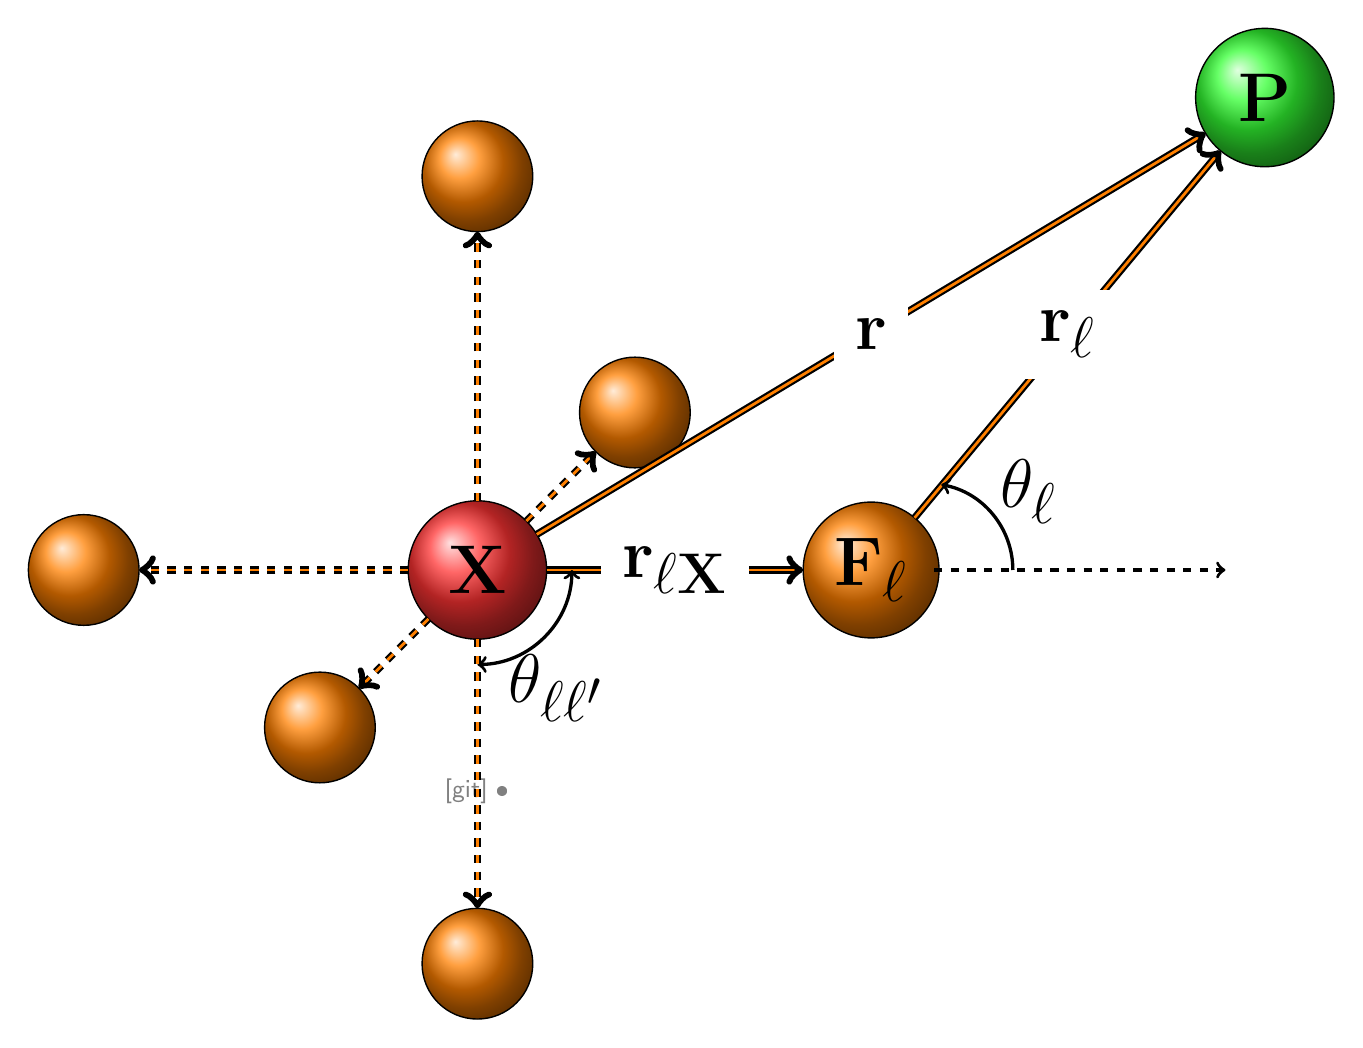
\begin{tikzpicture}
\GraphInit[vstyle = Shade]
\Huge
\tikzset{
  % LabelStyle/.style = {font = \bfseries},
  VertexStyle/.append style = { inner sep=5pt, minimum size=40pt ,
                                font = \bfseries},
  EdgeStyle/.append style = {->},
}

  \SetGraphUnit{5}
  \begin{scope}
    \tikzset{VertexStyle/.append style = {%
        shape= circle, shading= ball, ball color= red!80!white,%
        minimum size = 50pt,draw} } 
    \Vertex[L=X]{X}
  \end{scope}


  \EA[L=$\bf{F}_{\ell}$](X){F}
  \WE[NoLabel](X){C}
  \NO[NoLabel](X){D}
  \SO[NoLabel](X){E}

  \Vertex[x=2, y=2, NoLabel]{A}
  \Vertex[x=-2, y=-2, NoLabel]{B}
  
  \begin{scope}
    \tikzset{VertexStyle/.append style = {%
      shape= circle,shading= ball,ball color= green!80!white,%
      minimum size = 50pt,draw}
    }
    \Vertex[x=10, y=6]{P}
  \end{scope}

  \Edge[label = $\bf{r}_{\ell X}$](X)(F)
  \Edge[label = $\bf{r}_{\ell}$](F)(P)
  \Edge[label = $\bf{r}$](X)(P)
  

  \tikzset{EdgeStyle/.append style = {->, dashed}}

  \draw [->,very thick, dashed] (5.8,0) -- (9.5,0);
  \draw [->, very thick] (6.8,0) arc [start angle=0, end angle=80, radius=1.1];
  \node at (7.,1) {$\theta_{\ell}$};

  \draw [<->, very thick] (0.,-1.2) arc [start angle=-90, end angle=0, radius=1.2];
  \node at (1,-1.5) {$\theta_{\ell \ell'}$};

  \Edge(X)(C)
  \Edge(X)(D)
  \Edge(X)(E)
  \Edge(X)(A)
  \Edge(X)(B)

\end{tikzpicture}


}
    \centering 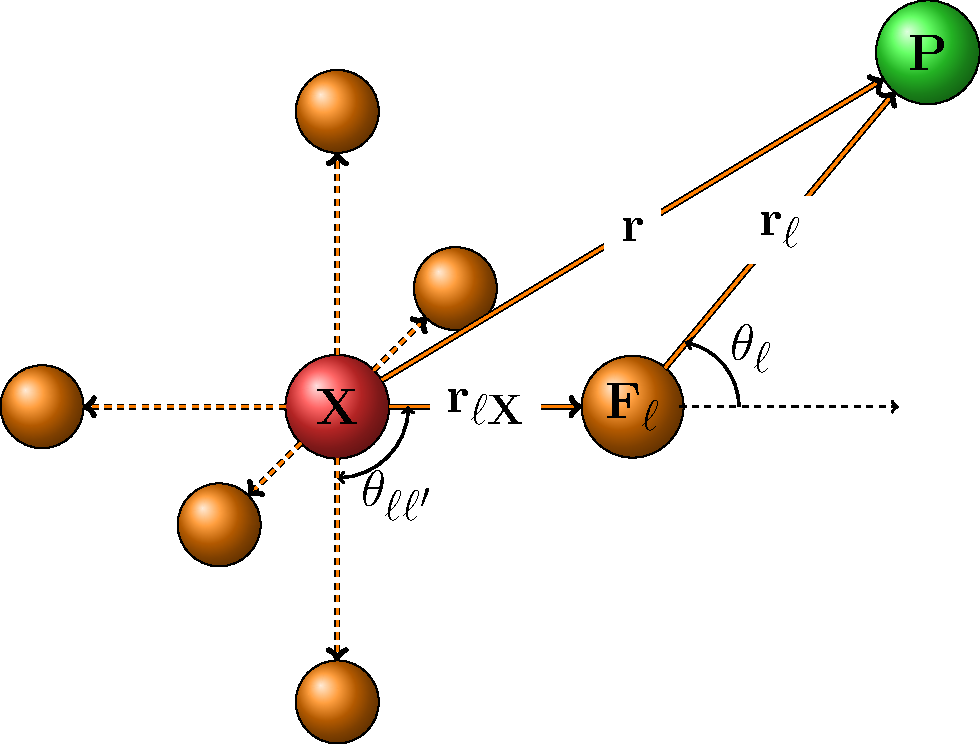
\includegraphics[width=.8\linewidth]{figures/coordenadas}
    \caption{Coordenadas utilizadas}
\end{minipage}\hfill
\begin{minipage}{0.5\textwidth}
  \begin{subequations}
    \begin{align}
      &\vect{r}=  \vect{r}_{\ce{P}} - \vect{r}_{X} , \\
      &\vect{r}_{\ell}=  \vect{r}_{\ce{P}} - \vect{r}_{\ce{F_{\ell}}} , \\
      &\vect{r}_{\ell X}= \vect{r}_{F_{\ell}} - \vect{r}_{X} ,
    \end{align}
  \end{subequations}
  \begin{itemize}
  \item $\theta_{\ell}$ es el \'{a}ngulo entre $\vect{r}_{\ell}$ y $\vect{r}_{\ell X}$,
  \item $\theta_{\ell \ell'}$ es el \'{a}ngulo entre $\vect{r}_{\ell}$ y $\vect{r}_{\ell'}$.
  \end{itemize}
\end{minipage}
\end{figure}

En el caso de colisiones de mol\'{e}culas de hexafluoruro de azufre (\ce{XF6}=\ce{SF6}) con un proyectil at\'{o}mico (en este caso $P=\ce{Ar}$) utilizamos para los potenciales intermoleculares las expresiones funcionales del grupo de Le Roy \autocite{Eichena1988TJCPp2898} y colaboradores (ver informe de Javier)
\begin{subequations}
  \begin{align} \label{Q:pot-inter-energy-1}
    U_{\ce{Ar-S}} &= - \sum_{n=3}^{5} \left[ 1 - \rme^{-br} \sum_{k=0}^{2n}\frac{(br)^{k}}{k!}\right] \frac{C_{2n}}{r^{2n}} \,,    \\
 \label{Q:pot-inter-energy-2}   U_{\ce{Ar-F_{\ell}}} &= A \Big[1 + p\, P_{2}(\cos \theta_{\ell})\Big]\, \rme^{-b r_{\ell}} - \sum_{n=3}^{5} \left[ 1 - \rme^{-br_{\ell}} \sum_{k=0}^{2n}\frac{(br_{\ell})^{k}}{k!}\right] \frac{C_{2n}}{r_{\ell}^{2n}}\,,
  \end{align}
\end{subequations}
$P_{2}(x)= 3 x^{2}/2 -1/2$ es el polinomio de Legendre de segundo orden.


\section{Fuerzas}
\label{S:calculo-fuerzas}
Las fuerzas se obtienen de las expresiones para la energ\'{\i}a potencial. Usaremos la aproximaci\'{o}n de que el potencial se puede escribir como una suma sobre potenciales de interacci\'{o}n de a pares entre \'{a}tomos. 

\subsection{Fuerzas intramoleculares}
Las fuerzas intra-moleculares se obtienen derivando la energ\'{\i}a (\ref{Q:pot-inter-energy-1}) y (\ref{Q:pot-inter-energy-2}) respecto a la coordenada respectiva:
%
\begin{subequations}
  \begin{align}\label{Q:F-sobre-X}
    &  \vect{F}^{\text{(i)}}_{X} = \sum_{\ell=1}^{6}\vect{F}^{\text{(i)}}_{X\ell} & \vect{F}^{\text{(i)}}_{X\ell} &=  2 K_{R} \, (r_{\ell X}- r_{0})\, \vers{r}_{\ell X}  \\
    & &  \vect{F}^{\text{(i)}}_{X\ell,i} &= 2 K_{R} \, \left( 1-\frac{r_{0}}{r_{\ell X}} \right) r_{\ell X,i}  \nonumber\\
    \label{Q:F-Sobre-Fl}
    &\vect{F}^{\text{(i)}}_{\ell} =   \vect{F}^{\text{(i)}}_{\ell X} + \sum_{\ell' \ne \ell} \vect{F}^{\text{(i)}}_{\ell \ell'} & \\
    &  & \vect{F}^{\text{(i)}}_{\ell X} &= -  \vect{F}^{\text{(i)}}_{X\ell} \nonumber \\
    & & \vect{F}^{\text{(i)}}_{\ell \ell'} &= -\frac{2 K_{\theta}}{r_{\ell X}} \frac{\theta_{\ell\ell'}-\theta_{0}}{\sin \theta_{\ell\ell'}} \Big[ \vers{r}_{\ell' X} - \cos{(\theta_{\ell\ell'})} \vers{r}_{\ell X} \Big] \nonumber
  \end{align}
\end{subequations}

\subsection{Fuerzas intermoleculares}

Como se muestra en el ap\'{e}ndice \ref{S:calculo-explicit-fuerzas} las fuerzas debidas a la presencia del proyectil est\'{a}n dadas por (\ref{Q:pot-inter-fuerzas}) y (\ref{Q:pot-inter-fuerza-S})

\begin{subequations}
  \begin{align}
    \label{Q:fuerzas-intermolec-resumen}
    \vect{F}^{\text{(e)}}_{\ell} =& - 3 A p \cos \theta_{\ell}\, \rme^{-b r_{\ell}} \vect{\Lambda} - A b \Big[1 + p\, P_{2}(\cos \theta_{\ell})\Big]\,\rme^{-b r_{\ell}} \vers{r_{\ell}} \nonumber \\
                                  &- \vers{r}_{\ell}\, \sum_{n=3}^{5} \frac{2 n\, C_{2n}}{r_{\ell}^{2n+1}} \,\left[ 1 - \frac{\rme^{-br_{\ell}}}{r_{\ell}} \left( \sum_{k=0}^{2n}\frac{(br_{\ell})^{k}}{k!} + \frac{(br_{\ell})^{2n+1}}{(2n)(2n)!} \right) \right] \\
    \vect{F}^{\text{(e)}}_{X} =&  3 A p \sum_{\ell=1}^{6} \cos \theta_{\ell}\, \rme^{-b r_{\ell}} \, \vect{\lambda} \\
    \vect{F}^{\text{(e)}}_{P} =& - \Bigl[ \vect{F}^{\text{(e)}}_{X} + \sum_{\ell} \vect{F}^{\text{(e)}}_{\ell}  \Bigr]
                                 \intertext{con}
                                  & \vect{\Lambda} = \left( \frac{1}{r_{\ell}} + \cos \theta_{\ell}\frac{1}{r_{\ell X}} \right) \vers{r}_{\ell X} - \left( \frac{1}{r_{\ell X}} + \cos \theta_{\ell}\frac{1}{r_{\ell}} \right) \vers{r}_{\ell} \\
                                  & \vect{\lambda}= \frac{1}{r_{\ell X}} \bigl( \vers{r}_{\ell} - \cos \theta_{\ell}\vers{r}_{\ell X} \bigr)
  \end{align}
\end{subequations}

\section{C\'{a}lculo del Jacobiano}
\label{S:calc-jacob}

El jacobiano del sistema de ecuaciones diferenciales para $N$ part\'{\i}culas interactuantes es una matriz de $6N \times 6N$, y tiene la forma
\begin{equation}
  \label{Q:Jacob-ec-dif}
  J =
  \begin{pmatrix}
    0 & A \\
    B & 0 \\
  \end{pmatrix}
\end{equation}
donde, en nuestro caso para \ce{XF6} con un proyectil $P=\ce{Ar}$, $N=8$, y la matriz $A$ est\'{a} formada por 8 bloques de $3 \times 3$, proporcionales a la identidad
\begin{align}
  \label{Q:Jacob-ec-dif-A}
  A &=
\begin{pmatrix}
  A_{X} & 0 & \cdots &  \cdots & 0 \\
  0 & A_{\ce{F1}}& 0 & \cdots & 0 \\
  \vdots  & \vdots  & \ddots &  & \vdots  \\
  0 &  0 &\cdots &  A_{\ce{F6}} & 0 \\
  0 & 0 & \cdots & 0 & P
\end{pmatrix}    &A_{j} = \frac{1}{M_{j}} \oper{I}^{(3\times 3)}
\end{align}

La matriz $B$ es de $(24\times 24)$ y contiene las derivadas de las fuerzas.
%
\begin{subequations}
  \begin{align}
    \label{Q:Jacob-eq-dif-B}
&   B =
\begin{pmatrix}
  BXX & BXF & BXP \\
  BFX & BFF & BFP \\
  BPX & BPF & BPP 
\end{pmatrix}   \\ \label{Q:Jacob-eq-dif-BXX}
    & BXX  & (BXX)_{i,j} = \frac{\partial F_{X,i}}{\partial r_{X,j}}  \\
\label{Q:Jacob-eq-dif-BXF}    &BXF =  \begin{pmatrix}   BXF_{1} & BXF_{2} & \cdots & BXF_{6}   \end{pmatrix}
    & (BXF_{\ell})_{i,j}=  \frac{\partial F_{X,i}}{\partial r_{\ell,j}}\\
\label{Q:Jacob-eq-dif-BFX}    &BFX =  \begin{pmatrix}   BF_{1}X \\ BF_{2}X \\ \cdots \\ BF_{6}X   \end{pmatrix}
    & (BF_{\ell}X)_{i,j}=  \frac{\partial F_{\ell,i}}{\partial r_{X,j}} \\ 
\label{Q:Jacob-eq-dif-BFF}    &BFF =  \begin{pmatrix}
  B11 & B12 & \cdots & B16 \\
  B21 & B22 & \cdots & B26 \\
  \vdots  & \vdots  & \ddots & \vdots  \\
  B61 & B62 & \cdots & B66 
 \end{pmatrix} & (B\ell\ell')_{i,j}=  \frac{\partial F_{\ell,i}}{\partial r_{\ell',j}}
  \end{align}
\end{subequations}
Usaremos la notaci\'{o}n $r_{X,i}$ para la componente $i=1,2,3$ (o sea $x,y,z$) del vector posici\'{o}n de la mol\'{e}cula $X$, e id\'{e}nticamente usaremos $r_{\ell, i}$ para la componente $i$ del vector posici\'{o}n del fl\'{u}or n\'{u}mero $\ell$. Similar notaci\'{o}n usamos para las componentes de la fuerza: $F_{X,i}$ es la componente $i$ de la fuerza total ejercida sobre el \'{a}tomo $X$.
Cada submatriz es de tama\~{n}o $3 \times 3$, donde $i,j= 1,2,3$  y $\ell,\ell'=1, \dots, 6$.

Las submatrices ($3 \times 3$) relacionadas con el proyectil tienen la forma 
\begin{align}
 & (BXP)_{i,j} =  \frac{\partial F_{X,i}}{\partial r_{P,j}} &
 & (BPX)_{i,j} =  \frac{\partial F_{P,i}}{\partial r_{X,j}} &  (BPP)_{i,j}=\frac{\partial F_{P,i}}{\partial r_{P,j}} \nonumber \\
\\
 & (BPF_{\ell})_{i,j}=  \frac{\partial F_{P,i}}{\partial r_{\ell,j}} &
 & (BF_{\ell}P)_{i,j}=  \frac{\partial F_{\ell,i}}{\partial r_{P,j}} & \forall \ell= 1, \dots, 6 \nonumber
\end{align}




\subsection{Relaciones entre los elementos de matriz}
\label{S:relaciones-elementos}


\subsubsection{Relaciones entre $BFX$, $BXF$ y $BXX$}
Para calcular $BFX$ consideramos como depende la fuerza sobre el \'{a}tomo \ce{X}  de la posici\'{o}n del fl\'{u}or $\ell$. 
Usamos que $\vect{r}_{\ell X} = \vect{r}_{\ell} - \vect{r}_{X}$
\begin{equation}
  \label{Q:BXF-1}
  (BXF_{\ell})_{ij} = \frac{\partial F_{X,i}}{\partial r_{\ell,j}} = \frac{\partial F_{X,i}}{\partial r_{\ell X,j}} \overbrace{\frac{\partial r_{\ell X,j}}{\partial r_{\ell,j}}}^{1} = \sum_{\ell'=1}^{6} \frac{\partial F_{X\ell',i}}{\partial r_{\ell X,j}} = \frac{\partial F_{X\ell,i}}{\partial r_{\ell X,j}}
\end{equation}

Para calcular el t\'{e}rmino $BF_{\ell}X$ debemos tener como var\'{\i}a la fuerza sobre el fl\'{u}or $\ell$ debido a movimientos de la posici\'{o}n del \'{a}tomo \ce{X}. En ese c\'{a}lculo debemos tener en cuenta que el \'{a}ngulo $\theta_{\ell \ell'} $ depende de la posici\'{o}n de \ce{X}.
Veamos si podemos pensarlo en forma diferente
\begin{equation}
  \label{Q:BFX-1}
  (BF_{\ell}X)_{ij} = \frac{\partial F_{\ell,i}}{\partial r_{X,j}} = \frac{\partial}{\partial r_{X,j}} \left(- \frac{\partial V}{\partial r_{\ell,i}}  \right) =
 \frac{\partial}{\partial r_{\ell,i}} \left(- \frac{\partial V}{\partial r_{X,j}}  \right) =  \frac{\partial F_{X,j}}{\partial r_{\ell,i}} = (BXF_{\ell})_{ji}
\end{equation}
por lo que tendremos $BFX=(BXF)^{t}$.

Para calcular $BXX$ consideramos el cambio en la fuerza sobre \ce{X} cuando var\'{\i}a su posici\'{o}n
\begin{equation}
  \label{Q:BXX-1}
  (BXX)_{ij} = \frac{\partial F_{X,i}}{\partial r_{X,j}} = \frac{\partial F_{X,i}}{\partial r_{\ell X,j}} \overbrace{\frac{\partial r_{\ell X,j}}{\partial r_{X,j}}}^{-1} = - \sum_{\ell=1}^{6} \frac{\partial F_{X\ell,i}}{\partial r_{\ell X,j}} = -\sum_{\ell=1}^{6} (BXF_{\ell})_{ij}
\end{equation}

\subsubsection{Relaciones entre $BFP$, $BPF$ y $BPP$}

Id\'{e}nticamente a la derivaci\'{o}n de las relaciones anteriores obtenemos
\begin{subequations}
  \begin{align}
    BPX &= (BXP)^{t}\\
    BPF_{\ell} &= (BF_{\ell}P)^{t} \\
    BPP &= - \sum_{\ell=1}^{6} {BF_{\ell}P} - BXP
  \end{align}
\end{subequations}

\subsubsection{Relaciones de submatrices en $BFF$}

En general, de (\ref{Q:Jacob-eq-dif-BFF}) podemos ver que:
\begin{equation}
  \label{Q:BFF-1}
  (B\ell\ell')_{ij} =  \frac{\partial F_{\ell,i}}{\partial r_{\ell',j}} = \frac{\partial}{\partial r_{\ell,j}} \left(- \frac{\partial V}{\partial r_{\ell',i}}  \right) =
 \frac{\partial}{\partial r_{\ell',i}} \left(- \frac{\partial V}{\partial r_{\ell,j}}  \right) =  \frac{\partial F_{\ell',j}}{\partial r_{\ell,i}} = (B\ell'\ell)_{ji} \,,
\end{equation}
% 
por lo que $B\ell\ell' = (B\ell'\ell)^{t}$.

Entonces, para $\ell = \ell'$ (matrices en la diagonal) $B\ell\ell = (B\ell\ell)^{t}$, y adem\'{a}s tendremos:
%
\begin{align*}
  (B\ell\ell)_{ij} =  \frac{\partial F_{\ell,i}}{\partial r_{\ell,j}} =  \frac{\partial }{\partial r_{\ell,j}} \left( {F}_{\ell X,i} + \sum_{\ell' \ne \ell} {F}_{\ell \ell',i} \right)
\intertext{donde}
   \frac{\partial F_{\ell X,i}}{\partial r_{\ell,j}} = - \frac{\partial F_{X \ell,i}}{\partial r_{\ell,j}} = - \frac{\partial F_{X \ell,i}}{\partial r_{\ell X,j}} \overbrace{\left( \frac{\partial r_{\ell X,j}}{\partial r_{\ell,j}} \right) }^{1} = - (BXF_{\ell})_{ij}
\intertext{y}
   \sum_{\ell' \ne \ell} \frac{\partial F_{\ell \ell',i}}{\partial r_{\ell,j}} = -  \sum_{\ell' \ne \ell} \frac{\partial F_{\ell' \ell,i}}{\partial r_{\ell,j}} = - \sum_{\ell' \ne \ell} (B\ell'\ell)_{ij}
\end{align*}
Por lo que
\begin{equation}
  \label{Q:BFF-diag-1}
  (B\ell\ell)_{ij} = (B\ell\ell)_{ji} = - (BXF_{\ell})_{ij} - \sum_{\ell' \ne \ell}(B\ell'\ell)_{ij}
\end{equation}

\subsection{C\'{a}lculos de los elementos de matrix intramoleculares}
\label{S:calc-de-elementos}

De los resultados de la secci\'{o}n anterior vemos que s\'{o}lo necesitamos calcular las expresiones (\ref{Q:Jacob-eq-dif-BXF}) y (\ref{Q:Jacob-eq-dif-BFF}) para $\ell' \ne \ell$
\begin{equation}
  \label{Q:Jac-deriv-BXF}
  \frac{\partial F_{X,i}}{\partial r_{\ell,j}} = 2 K_{R} \left[\left( 1 - \frac{r_{0}}{r_{\ell X}} \right)\delta_{ij}  + \frac{r_{0}}{r_{\ell X}^{3}} r_{\ell X,i} r_{\ell X,j}\right]
\end{equation}

\begin{equation}
  \label{Q:Jac-deriv-BFF}
  \frac{\partial F_{\ell,i}}{\partial r_{\ell',j}} = \frac{\partial F_{ \ell \ell',i}}{\partial r_{\ell'X,j}} = - \frac{2 K_{\theta}}{r_{\ell}} \frac{\partial}{\partial r_{\ell',j}}\left[\frac{\theta -\theta_{0}}{\sin \theta} \Big( \frac{r_{\ell',i}}{r_{\ell'}} - \frac{r_{\ell,i}}{r_{\ell}} \cos{\theta} \Big)  \right]
\end{equation}
donde simplificamos la notaci\'{o}n, usando en el miembro de la derecha $\theta\equiv \theta_{\ell\ell'}$, $r_{\ell X}\equiv r$ y  $r_{\ell' X}\equiv r'$.

Calculando expl\'{\i}citamente obtenemos:
\begin{subequations}
  \begin{align}
    \frac{\partial F_{ \ell \ell',i}}{\partial r'_{j}} &= - \frac{2 K_{\theta}}{r} \left\{\left[\frac{r'_{i}}{r'} - \cos \theta \frac{r_{i}}{r}\right] \frac{\partial}{\partial r'_{j}}\left( \frac{(\theta - \theta_{0})}{\sin \theta} \right) + \frac{\theta - \theta_{0}}{\sin \theta} \left[ \frac{\partial (r'_{i}/r') }{\partial r'_{j}} -  \frac{r_{i}}{r}\frac{\partial (\cos \theta)}{\partial r'_{j}}  \right] \right\}
%
\intertext{con}
& \frac{\partial (r'_{i}/r')}{\partial r'_{j}} = \frac{1}{r'}\delta_{ij} - \frac{r'_{i} r'_{j}}{r'^{3}} \\  
& \frac{\partial}{\partial r'_{j}}\left( \frac{(\theta - \theta_{0})}{\sin \theta} \right) = \frac{\sin \theta - (\theta -\theta_{0})\, \cos \theta }{\sin^{2} \theta} \; \frac{\partial \theta}{\partial r'_{j}} 
\\
&  \frac{\partial \theta}{\partial r'_{j}} = \frac{-1}{\sin \theta}\, \frac{\partial (\cos \theta)}{\partial r'_{j}} \\
                                                       & \frac{\partial (\cos \theta)}{\partial r'_{j}} = \frac{1}{r'}\left( \frac{r_{j}}{r} - \cos \theta\, \frac{r'_{j}}{r'} \right)
  \end{align}
\end{subequations}

\subsection{C\'{a}lculo de los elementos de Matriz intermoleculares}
\label{S:elementos-matriz-intermolec}

\subsubsection{Elementos $(BXX)^{(e)}$:}

Empezamos calculando las derivadas de la fuerza sobre el \'{a}tomo central debido a variaciones en su posici\'{o}n
\begin{subequations}
\begin{align}
  (BXX)^{(e)}_{ij} &= \frac{\partial F^{(e)}_{X,i}}{\partial r_{X,j}} = \frac{\partial F^{(e)}_{X,i}}{\partial r_{\ell X,j}} \overbrace{\frac{\partial r_{\ell X,j}}{\partial r_{X,j}}}^{-1} \nonumber\\
&= 3 A p \, \sum_{\ell} e^{-br_{\ell}} \, \Biggl\{\frac{1}{r_{\ell}}  \overbrace{\frac{\partial}{\partial r_{\ell X,j}} \left(\cos \theta_{\ell} \frac{r_{\ell X,i}}{r_{\ell X}} \right)}^{A} + \overbrace{\frac{\partial}{\partial r_{\ell X,j}} \left(\cos^{2} \theta_{\ell}\, \frac{r_{\ell X,i}}{r_{\ell X}^{2}} \right)}^{B} \biggr\}
\intertext{donde }
    A &= \frac{r_{\ell X,i}}{r_{\ell X}} \left( \frac{\partial \cos \theta_{\ell}}{\partial r_{\ell X,j}} \right)  + \cos \theta_{\ell} \frac{\partial ({r_{\ell X,i}}/{r_{\ell X}})}{\partial r_{\ell X,j}}  \, \\
    B&= 2 \cos \theta_{\ell} \frac{r_{\ell X,i}}{r^{2}_{\ell X}}\left( \frac{\partial \cos \theta_{\ell}}{\partial r_{\ell X,j}} \right)  + \cos^{2} \theta_{\ell}\frac{\partial ({r_{\ell X,i}}/{r^{2}_{\ell X}})}{\partial r_{\ell X,j}}
       \intertext{con}
     & \frac{\partial \cos \theta_{\ell}}{\partial r_{\ell X,j}}= \frac{1}{r_{\ell X}} \left[\frac{r_{\ell,j}}{r_{\ell}} - \cos{\theta_{\ell}} \frac{r_{\ell X,j}}{r_{\ell X}}\right] \\
\label{Q:deriv-i_r}
      & \frac{\partial ({r_{\ell X,i}}/{r_{\ell X}})}{\partial r_{\ell X,j}} = \frac{\delta_{ij}}{r_{\ell X}} - \frac{r_{\ell X,i} r_{\ell X,j}}{r_{\ell X}^{3}} \\
\label{Q:deriv-i_r2}
      & \frac{\partial ({r_{\ell X,i}}/{r^{2}_{\ell X}})}{\partial r_{\ell X,j}} =\frac{1}{r_{\ell X}}\, \left[\frac{\delta_{ij}}{r_{\ell X}} - 2 \frac{r_{\ell X,i} r_{\ell X,j}}{r_{\ell X}^{3}} \right]
  \end{align}
\end{subequations}

\subsubsection{Elementos $(BXF_{\ell})^{(e)}$:}
Derivada de la fuerza sobre $X$ debido a movimientos de un fl\'{u}or:
%
\begin{subequations}
  \begin{align}
    (BXF_{\ell})^{(e)}_{ij} &= \frac{\partial F^{(e)}_{X,i}}{\partial r_{F_{\ell},j}} \\
&= -3 A p \, \Biggl\{ \overbrace{\frac{\partial}{\partial r_{F_{\ell},j}} \left[{\cos {\theta_{\ell}}}\, \frac{\rme^{-b r_{\ell}}}{r_{\ell}}\, \frac{r_{\ell X,i}}{r_{\ell X}}\right]}^{C} + \overbrace{\frac{\partial}{\partial r_{F_{\ell},j}} \left[{\cos^{2}{\theta_{\ell}}} \,\rme^{-b r_{\ell}}\, \frac{r_{\ell X,i}}{r_{\ell X}^{2}} \right]}^{D}\biggr\} 
    % \nonumber
    \intertext{donde }
    C =& \frac{\rme^{-b r_{\ell}}}{r_{\ell}}\,\Biggl[ \frac{r_{\ell X,i}}{r_{\ell X}} \overbrace{\frac{\partial \cos \theta_{\ell}}{\partial r_{F_{\ell},j}} }^{\Lambda_{j}} +
    \cos \theta_{\ell} \frac{r_{\ell X,i}}{r_{\ell X}} \left[b + \frac{1}{r_{\ell}}\right] 
    +
    \cos \theta_{\ell} \overbrace{\frac{\partial (r_{\ell X,i}/r_{\ell X})}{\partial r_{\ell X,j}} }^{(\ref{Q:deriv-i_r})}\Biggr] \\
    D =& \rme^{-b r_{\ell}} \cos \theta_{\ell} \Biggl[2 \frac{r_{\ell X,i}}{r^{2}_{\ell X}} \overbrace{\frac{\partial \cos \theta_{\ell}}{\partial r_{F_{\ell},j}} }^{\Lambda_{j}} +
      b \cos \theta_{\ell} \frac{r_{\ell X,i}}{r^{2}_{\ell X}} \frac{r_{\ell,j}}{r_{\ell}}
    +
 \cos \theta_{\ell} \overbrace{\frac{\partial (r_{\ell X,i}/r^{2}_{\ell X})}{\partial r_{\ell X,j}} }^{(\protect\ref{Q:deriv-i_r2})} \Biggr]
  \end{align}
\end{subequations}
%
% donde $\Lambda_{j}$ se defini\'{o} en (\ref{Q:def-Dcos}).

% % \begin{align}
% %   =& -3 A p \,\frac{\rme^{-b r_{\ell}}}{r_{\ell X}}\,\Biggl\{ D_{j} \frac{r_{\ell X,i}}{r_{\ell}} + \cos \theta_{\ell} \frac{b r_{\ell} + 1}{r_{\ell}} \frac{r_{\ell,j} r_{\ell X,i}}{r_{\ell}^{2}} + \frac{\cos \theta_{\ell}}{r_{\ell}} \left( \delta_{ij} -  \frac{r_{\ell,j} r_{\ell X,i}}{r_{\ell X}^{2}} \right) \nonumber \\
% %    &+ 2 \cos \theta_{\ell} \, D_{j} \frac{r_{\ell X,i}}{r_{\ell X}} - b \cos^{2}{ \theta_{\ell}} \frac{r_{\ell,j} r_{\ell X,i}}{r_{\ell} r_{\ell X}}  +  \frac{\cos^{2}{ \theta_{\ell}}}{r_{\ell X}} \left( \delta_{ij} -  \frac{2 r_{\ell,j} r_{\ell X,i}}{r_{\ell X}^{2}} \right) \biggr\}
% % \end{align}

% \begin{align}
%   (BF_{\ell}F_{\ell})^{(e)}_{ij} &= \frac{\partial F^{(e)}_{\ell,i}}{\partial r_{\ell,j}} \\&= -3 A p 
% \end{align}


\begin{subappendices}
\section{C\'{a}lculo expl\'{\i}cito de las fuerzas}
\label{S:calculo-explicit-fuerzas}


\subsection{C\'{a}lculo de Fuerzas intermoleculares}


\subsubsection{Fuerzas sobre los \'{a}tomos de fl\'{u}or}

Las fuerzas sobre los \'{a}tomos de fl\'{u}or se obtienen derivando respecto a la coordenada respectiva:
\begin{subequations}
\begin{align} \label{Q:fuerzas-intermolec}  
  \frac{\partial U_{\ce{Ar-F_{\ell}}}}{\partial r_{F_{\ell},i}} &= \frac{\partial U_{1}}{\partial r_{F_{\ell},i}} + \frac{\partial U_{2}}{\partial r_{F_{\ell},i}}
 \intertext{con}
U_{1}&=  A \Big[1 + p\, P_{2}(\cos \theta_{\ell})\Big]\, \rme^{-b r_{\ell}} & U_{2}= \sum_{n=3}^{5} \left[ 1 - \rme^{-br_{\ell}} \sum_{k=0}^{2n}\frac{(br_{\ell})^{k}}{k!}\right] \frac{C_{2n}}{r_{\ell}^{2n}}\,.
\end{align}
\end{subequations}
El primer t\'{e}rmino es:
\begin{equation}
 \label{Q:pot-inter-dU1}
 \frac{\partial U_{1}}{\partial r_{F_{\ell},i}} &= 3 A p \cos \theta_{\ell}\, \rme^{-b r_{\ell}} \frac{\partial \cos \theta_{\ell}}{\partial r_{F_{\ell},i}} - A b \Big[1 + p\, P_{2}(\cos \theta_{\ell})\Big]\,\rme^{-b r_{\ell}} \frac{\partial r_{\ell}}{\partial r_{F_{\ell},i}} \,.
\end{equation}
El Jacobiano debido al cambio de coordenada es simple, y la escribimos para referencia futura
\begin{equation}\label{Q:der_rl_rFl}
  \frac{\partial r_{\ell}}{\partial r_{F_{\ell},i}} =   \frac{\partial r_{\ell}}{\partial r_{\ell,i}}   \overbrace{\frac{\partial r_{\ell, y}}{\partial r_{F_{\ell},i}}}^{-1} = -\frac{\partial r_{\ell}}{\partial r_{\ell,i}} = -\frac{r_{\ell, i}}{r_{\ell}}
\end{equation}
%
Para calcular la derivada del coseno, tenemos en cuenta que $\cos \theta_{\ell} = \vect{r}_{\ell} \cdot \vect{r}_{\ell X}/r_{\ell} r_{\ell X}$. Entonces podemos calcular:
\begin{subequations}
  \begin{align}\label{Q:pot-inter-deriv-cos}
    \Lambda_{i}&= \frac{\partial \cos \theta_{\ell}}{\partial r_{F_{\ell},i}} = \left( \frac{1}{r_{\ell}} + \cos \theta_{\ell}\frac{1}{r_{\ell X}} \right) \frac{r_{\ell X,i}}{r_{\ell X}} -
                 \left( \frac{1}{r_{\ell X}} + \cos \theta_{\ell}\frac{1}{r_{\ell}} \right) \frac{r_{\ell,i}}{r_{\ell}} 
 \intertext{y vectorialmente}
%
 \label{Q:pot-inter-deriv-cos-vect} \vect{\Lambda} &= \left( \frac{1}{r_{\ell}} + \cos \theta_{\ell}\frac{1}{r_{\ell X}} \right) \vers{r}_{\ell X} - \left( \frac{1}{r_{\ell X}} + \cos \theta_{\ell}\frac{1}{r_{\ell}} \right) \vers{r}_{\ell}
  \end{align}
\end{subequations}
%
por lo que la ec.~(\ref{Q:pot-inter-dU1}) se escribe:
\begin{equation}\label{Q:pot-inter-dU1}
  \frac{\partial U_{1}}{\partial r_{F_{\ell},i}} = A \left[3 p \Lambda_{i} \cos \theta_{\ell} + b \Big[1 + p\, P_{2}(\cos \theta_{\ell})\Big]\,\frac{r_{\ell, i}}{r_{\ell}}\right] \rme^{-b r_{\ell}} 
\end{equation}

Calculemos ahora el segundo t\'{e}rmino
\begin{equation*}
  \frac{\partial U_{2}}{\partial r_{F_{\ell},i}} = \left\{\sum_{n=3}^{5} \frac{\partial}{\partial r_{\ell}}\left[ 1 - \rme^{-br_{\ell}} \sum_{k=0}^{2n}\frac{(br_{\ell})^{k}}{k!}\right] \frac{C_{2n}}{r_{\ell}^{2n}} + \left[ 1 - \rme^{-br_{\ell}} \sum_{k=0}^{2n}\frac{(br_{\ell})^{k}}{k!}\right] \frac{\partial}{\partial r_{\ell}}\left[ \frac{C_{2n}}{r_{\ell}^{2n}}\right] \right\} \, \left(- \frac{\partial r_{\ell}}{\partial r_{F_{\ell},i}} \right)
\end{equation*}
%
donde, la derivada en el primer t\'{e}rmino se puede calcular como:
\begin{align*}
 \frac{\partial}{\partial r_{\ell}}\left[ 1 - \rme^{-br_{\ell}} \sum_{k=0}^{2n}\frac{(br_{\ell})^{k}}{k!}\right] &= - \left\{(-b) \rme^{-br_{\ell}} \sum_{k=0}^{2n}\frac{(br_{\ell})^{k}}{k!} + \rme^{-br_{\ell}} b \, { \sum_{k=0}^{2n}  k \frac{(br_{\ell})^{k-1}}{k!}} \right\} 
\\
&\bajo{=}{k'=k-1}  b \rme^{-br_{\ell}} \left[\sum_{k=0}^{2n}\frac{(br_{\ell})^{k}}{k!} - \sum_{k'=0}^{2n-1} \frac{(br_{\ell})^{k'}}{k'!}\right] 
\\
&=  b \rme^{-br_{\ell}} \frac{(b r_{\ell})^{2n}}{(2n)!}
\end{align*}
%
mientras que para el segundo calculamos:
\begin{equation*}
 \frac{\partial}{\partial r_{\ell}}\left[ \frac{C_{2n}}{r_{\ell}^{2n}}\right] = -\frac{2n}{r_{\ell}}\, \frac{C_{2n}}{r_{\ell}^{2n}} \,.
\end{equation*}
% y adem\'{a}s:
% \begin{equation*}
%   \frac{\partial r_{\ell}}{\partial r_{\ell,i}} = \frac{r_{\ell,i}}{r_{\ell}}
% \end{equation*}
%
Utilizando estos resultados y (\ref{Q:der_rl_rFl}) en la expresi\'{o}n anterior obtenemos
\begin{align}\label{Q:pot-inter-dU2}
  \frac{\partial U_{2}}{\partial r_{\ell,i}} &= \sum_{n=3}^{5} \left\{ -b \rme^{-br_{\ell}} \frac{(b r_{\ell})^{2n}}{(2n)!} + \frac{2n}{r_{\ell}} \left[ 1 - \rme^{-br_{\ell}} \sum_{k=0}^{2n}\frac{(br_{\ell})^{k}}{k!}\right] \right\}  \left[ \frac{C_{2n}}{r_{\ell}^{2n}}\right]\, \frac{r_{\ell,i}}{r_{\ell}} 
 % &=  \sum_{n=3}^{5} 2 n\, C_{2n} \,\left\{1 - \frac{\rme^{-br_{\ell}}}{r_{\ell}}  \left[ \sum_{k=0}^{2n}\frac{(br_{\ell})^{k}}{k!} + \frac{(br_{\ell})^{2n+1}}{(2n)(2n)!} \right] \right\} \frac{r_{\ell,i}}{r_{\ell}^{2(n+1)}}
\end{align}
\medskip

Finalmente, la fuerza sobre el \'{a}tomo $\ell$ ser\'{a} la suma de (\ref{Q:pot-inter-dU1}) y (\ref{Q:pot-inter-dU2}):
\begin{align} \label{Q:pot-inter-fuerzas}
    \vect{F}^{\text{(e)}}_{\ell} =& - 3 A p \cos \theta_{\ell}\, \rme^{-b r_{\ell}} \vect{\Lambda} - A b \Big[1 + p\, P_{2}(\cos \theta_{\ell})\Big]\,\rme^{-b r_{\ell}} \vers{r_{\ell}} \nonumber \\
                     &- \vers{r}_{\ell}\, \sum_{n=3}^{5} \frac{2 n\, C_{2n}}{r_{\ell}^{2n+1}} \,\left[ 1 - \frac{\rme^{-br_{\ell}}}{r_{\ell}} \left( \sum_{k=0}^{2n}\frac{(br_{\ell})^{k}}{k!} + \frac{(br_{\ell})^{2n+1}}{(2n)(2n)!} \right) \right] 
\end{align}
%
donde $\vect{\Lambda}$ fue definido en (\ref{Q:pot-inter-deriv-cos-vect}).

\subsubsection{Fuerzas sobre el \'{a}tomo central}

La contribuci\'{o}n de la energ\'{\i}a $U_{\ce{Ar-F_{\ell}}}$ en la fuerza sobre el \'{a}tomo central (de azufre en este caso) viene de la dependencia del coseno del \'{a}ngulo $\theta_{\ell}$ con la coordenada $\vect{r}_{X}$,
\begin{subequations}
  \begin{align}
    \label{Q:pot-inter-fuerza-S}
    \vect{F}^{\text{(e)}}_{X} = -\frac{\partial U_{1}}{\partial r_{X,i}} &= -\sum_{\ell=1}^{6} \frac{\partial U_{1}}{\partial r_{\ell X,i}} \overbrace{ \frac{\partial r_{\ell X,i}}{\partial r_{X,i}}}^{-1} = 3 A p \sum_{\ell=1}^{6} \cos \theta_{\ell}\, \rme^{-b r_{\ell}} \, \vect{\lambda}
    \intertext{con}
\lambda_{i} &=\frac{\partial \cos{\theta_{\ell}}}{\partial r_{\ell X,i}} \qquad\qquad   \vect{\lambda}= \frac{1}{r_{\ell X}} \bigl( \vers{r}_{\ell} - \cos \theta_{\ell}\vers{r}_{\ell X} \bigr) 
  \end{align}
\end{subequations}
Si despreciamos la fuerza ejercida directamente por el proyectil, esta es la fuerza total sobre el \'{a}tomo central.

\end{subappendices}

%%% Local Variables:
%%% mode: latex
%%% TeX-master: "main"
%%% End:



\part{Appendixes}
\appendix{}

\chapter{Three-body kinematics}

\section{Coordinate system}
\label{S:coord-syste}


Let us consider the collision of a projectile of mass $M_P$, charge $Z_P$ and velocity $\bm{v}$ (impulse $\bm{P} = M_P \bm{v}$) with a two-particle target of mass $M_T + m$ initially at rest in the laboratory reference system. Without any loss of generality we shall consider that $m \leq M_T$. The total energy is given by $E_{\rm Lab} = M_P v^2 / 2 + \varepsilon_i$, where $\varepsilon_i$ is the internal energy of the target. By extracting the constant energy $M v_{CM}^2 / 2$ associated with the movement with velocity $\bm{v}_{CM} = M_P \bm{v} / M$ of the whole system of mass $M = M_T + M_P + m$, we obtain the energy in the center-of-mass reference frame $E_i = \mu_T v^2 / 2 + \varepsilon_i$. Here $\mu_T = (m + M_T) M_P / (M_T + M_P + m)$ is the reduced mass of the initial projectile-target configuration.

In the center-of-mass reference system, the three-body problem can be described by any of three possible sets of Jacobi coordinates (Macek and Shakeshaft 1980),
\[
\vec{x}_T = \left( \begin{matrix} \bm{r}_T \cr \bm{R}_T \cr
  \end{matrix}
\right) \, , \, \vec{x}_P = \left( \begin{matrix} \bm{r}_P \cr \bm{R}_P \cr
  \end{matrix}
\right) \, , \, \vec{x}_N = \left( \begin{matrix} \bm{r}_N \cr \bm{R}_N \cr
  \end{matrix}
\right) \; ,
\]
as shown in \ref{f:jacobi}. In our notation, $\bm{r}_T$, $\bm{r}_P$ and $\bm{R}_N$ are the position vectors of the particle of mass $m$ relative to the recoiling target fragment T, the projectile P and the center of mass of T + P, respectively. $\bm{R}_P$ is the position vector of the centre of mass of $m$ + P relative to T; and $\bm{r}_N$ and $\bm{R}_T$ are the coordinates of P relative to T and the centre of mass of $m$ + T, respectively. These Jacobi coordinates are related by $\vec{x}_j = {\cal M}_{j \ell}\ \vec{x}_\ell$, for $j , \ell = T$, $P$ or $N$, with
\begin{eqnarray*} {\cal M}_{PT} = \left(\begin{matrix}\alpha & -1 \cr 1- \alpha \beta & \beta \cr
    \end{matrix}
  \right) & & \; {\cal
    M}_{TP} = \left( \begin{matrix} \beta & 1 \cr \alpha \beta - 1 & \alpha \cr 
    \end{matrix}
  \right) \\  {\cal
    M}_{NT} = \left(\begin{matrix} 1 - \alpha & 1 \cr \alpha + \gamma - \alpha \gamma & \gamma - 1 \cr
    \end{matrix}
  \right) \qquad & & \; {\cal M}_{TN} = \left(\begin{matrix}1 - \gamma & 1 \cr \alpha + \gamma - \alpha
      \gamma & \alpha - 1 \cr 
    \end{matrix}
  \right) \\  {\cal M}_{NP} = \left( \begin{matrix} \beta - 1 & 1 \cr 1-
      \gamma (1- \beta) & \gamma \cr 
    \end{matrix}
  \right) & & \; {\cal M}_{PN} = \left( \begin{matrix} -\gamma & 1 \cr 1
      - \gamma (1- \beta) & 1 - \beta \cr 
    \end{matrix}
  \right) \; ,
\end{eqnarray*}
where
\[
\qquad \alpha= \frac{M_T}{m + M_T} \qquad , \qquad \beta=\frac{M_P}{m + M_P} \qquad \mbox{and} \qquad \gamma = \frac{M_T}{M_P + M_T} \; .
\]
These pairs of coordinates diagonalize the free Hamiltonian $H_o$ in the center-of-mass reference frame.

In momentum space, the system is described by the associated pairs $(\bm{k}_T, \bm{K}_T)$, $(\bm{k}_P, \bm{K}_P)$ and $(\bm{k}_N,\bm{K}_N)$ which are related by
\[
\left( \begin{matrix} \bm{k}_j \cr \bm{K}_j \cr \end{matrix} \right) = {\cal M}^t_{\ell j} \left( \begin{matrix} \bm{k}_\ell \cr \bm{K}_\ell \cr
  \end{matrix}
\right) \; ,
\]
where the superscript $t$ indicates the transposition of the matrix elements.

Switching back to the Laboratory reference frame, $\bf k$, $\bm{K}_R$ and $\bm{K}$ are the final momenta of the electron of mass $m$, the (recoil) target fragment of mass $M_T$ and the projectile of mass $M_P$.

In the mass-restricted problems, it is assumed that the target nucleus remains motionless throughout the collision. Additionally, in the Poincar\'{e} restricted problem the projectile momentum $\bf K$ is bound to remain fixed at its initial value $M_{P} \bm{v}$. As a consequence, the electron momentum is identified either with the Jacobi electron-target momentum, $\bm{k} \equiv \bm{k}_{T}$, or with the electron-projectile momentum, $\bm{k} \equiv \bm{k}_{P}+ m \bm{v}$. In particular, the electron double-differential cross-section $d \sigma / d \bm{k}$ is assumed to be equal either to $d \sigma / d \bm{k}_T$ or $d \sigma / d \bm{k}_P$. However, this is not generally valid for any mass configuration. One of the main features of the present formulation is that we are not neglecting any $\alpha$, $\beta$ or $\gamma$ terms.  In our approach these parameters can be changed arbitrarily from very
small to very large numbers in order to cope with any possible mass configuration. However, each momentum in the laboratory reference frame can still be written in terms of a given Jacobi impulse $\bm{K}_j$ as
\begin{equation}\label{Q:1}
  \qquad \bm{k} = m \bm{v}_{CM} + \bm{K}_N \quad , \quad \bm{K} =
  M_P \bm{v}_{CM} + \bm{K}_T \quad \mbox{and} \quad \bm{K}_R = M_T
  \bm{v}_{CM} - \bm{K}_P \; ;
\end{equation}
so that, for instance, $d \sigma / d \bm{k} = d \sigma / d \bm{K}_N$. In general, the multiple-differential cross-section for ionization collisions in the impulse of the particles can be written in terms of the Jacobi impulses ($j=T$, $P$ o $N$),
\begin{equation}\label{Q:2}
  \frac
  {d \sigma} {d \bm{k} \, d \bm{K} \,d \bm{K}_R} = \delta
  \left( \bm{k} + \bm{K} + \bm{K}_R - M \bm{v}_{CM}\right) \, \frac {d
    \sigma} {d \bm{k}_j \, d \bm{K}_j} \; .
\end{equation}
Here (atomic units are used throughout)
\begin{equation}\label{Q:3}
  \frac {d \sigma} {d \bm{k}_j \, d \bm{K}_j}= \,
  \frac{(2\pi)^4}{v} |t_{if}|^2 \, \delta \left(E_i - \frac{1}{2 m_j}
    k_j^2 - \frac{1}{2 \mu_j} K_j^2 \right) \; ,
\end{equation}
where $t_{if}$ is the transition matrix element. We have defined the reduced masses of each two- and three-body system
\begin{eqnarray*}
  m_T = \alpha m = \frac{m M_T}{m + M_T} & & \; \mu_T = \frac {\beta m} {1 - \alpha \beta} =
  \frac{(m + M_T)M_P}{m + M_T + M_P} \\ m_P = \beta m = \frac{m M_P}{m + M_P} & & \; \mu _P = \frac
  {\alpha m} {1 - \alpha \beta} = \frac{(m + M_P) M_T}{m + M_T + M_P} \\ m_N=\gamma M_P = \frac{M_T
    M_P}{M_T + M_P} \qquad & & \; \mu_N = \frac{(M_P + M_T) m} {m + M_T + M_P} \; .
\end{eqnarray*}
such that
\[
m_j \mu_j = \frac {m M_T M_P} {m + M_T + M_P} \qquad \mbox{for $j$ = $N$, $T$ or $P$.}
\]

In terms of the laboratory momenta $\bm{k}, \bm{Q}$ the Jacobi momenta are written:
\begin{align*}
  \bm{k}_{T}&= \bm{k} - \frac{m_{T}}{M_{T}}\, \bm{Q} \,, &
  \bm{k}_{P}&= \frac{m_{P}}{m}\,\bm{k} + \frac{m_{P}}{M_{P}}\, \bm{Q} - m_{P}\bm{v} \, , &
  \bm{k}_{N}&= \frac{m_{N}}{M_{T}}\,\bm{k} -  \bm{Q} + m_{N}\bm{v} &
\end{align*}

%%% Local Variables: 
%%% mode: latex
%%% TeX-master: "mainxs"
%%% End: 

\chapter{CDW-B1: Summary of calculations}

\section*{The T-matrix ($t_{if} = t_{p} + t_{n}$)}

\begin{eqnarray}\label{QR:T}%
t_{P} &=& \frac{Z_{P}\, \mathcal{N}_{P} \mathcal{N}_{N}}{(2\pi)^{9/2}}
\; \lim_{\lambda_{1},\lambda_{2} \to 0^{+}} \mathcal{H} \left(
\lambda_{1},- \nu_{P},\bm{k}_{P} ;  \lambda_{2},-
\nu_{N},\bm{k}_{N};\bm{Q} , -(m_{T}/M_{T}) \, \bm{Q} \right)
  \nonumber \\
t_{N} &=& \frac{Z_{N} \, \mathcal{N}_{P} \mathcal{N}_{N}}{(2\pi)^{9/2}}
\; \lim_{\lambda_{1},\lambda_{2} \to 0^{+}} \mathcal{H} \left(
\lambda_{1}, - \nu_{N},\bm{k}_{N} ; \lambda_{2},- \nu_{P},\bm{k}_{P} ;
- \bm{Q} ,  (m_{T}/m) \, \bm{Q} \right) \; ,
\end{eqnarray}
%
where
%
\section{The $\mathcal{H}$ function (I)}
This expression regularize the singularity of $J_{0}$ in the origin by
using the volume element
%
\begin{equation}\label{Q:Ha}%
  \fbeq{
 \mathcal{H} \left( \lambda_{1},a_{1},\bm{k}_{1} ;
  \lambda_{2},a_{2},\bm{k}_{2}; \bm{Q}, \bm{p} \right)  =
 \int d \bm{q} \; F_{if}( \bm{p} + \bm{Q} - \bm{q} ) \;
 J_{1}( \lambda_{1}, \bm{q} - \bm{Q}, a_{1}, \bm{k}_{1} )\;
J_{0}( \lambda_{2}, \bm{q} , a_{2}, \bm{k}_{2} )
  }
\end{equation}

\subsection{Expansion around $\bi{q} = \bi{Q}$} 

This expansion will regularize the singularity of $J_{1}$
%
\[
\mathcal{H} = \mathcal{H}_{o} + \mathcal{H}_{1} + \Delta^{2}
\mathcal{H}
\]

\begin{equation}\label{Q:Hb}
\mathcal{H}_{o} \left( \lambda_{1},a_{1},\bm{k}_{1} ; \lambda_{2},
a_{2}, \bm{k}_{2} ; \bm{Q}, \bm{p} \right) = (2 \pi)^{3} \;
F_{if}(\bm{p}) \; N_{1} \left(\lambda_{1}+\lambda_{2}, \bm{Q} ; a_{1},
- \bm{k}_{1} ; a_{2}, \bm{k}_{2} \right)
\end{equation}
%
\[
\mathcal{H}_{1}\left( \lambda_{1},a_{1},\bm{k}_{1} ; \lambda_{2},
a_{2}, \bm{k}_{2}; \bm{Q}, \bm{p} \right)= (2 \pi)^{3} \, \bm{L}_{if}
(\bm{p}) \cdot  \left[ \bm{I}_{1}(\lambda,\bm{Q}; a_{1}, -\bm{k}_{1};
a_{2}, \bm{k}_{2} ) + i \bm{Q} N_{1}(\lambda,\bm{Q} ;
a_{1},-\bm{k}_{1} ; a_{2},\bm{k}_{2}) \vstretch \right]
\]
%
\[
\Delta^{2} \mathcal{H} = \int d \bm{q} \; \left\{ F_{if}( \bm{p} +
\bm{Q} - \bm{q} ) - F_{if}(\bm{p}) + i (\bm{q}-\bm{Q})
\bm{L}_{if}(\bm{p}) \vstretch\right\} \;
 J_{0}( \lambda_{2}, \bm{q} , a_{2}, \bm{k}_{2} ) \;
 J_{1}( \lambda_{1}, \bm{q} - \bm{Q}, a_{1}, \bm{k}_{1} )
\]

\section{The $\mathcal{H}$ function (II)}
This expression use the volume element for regularize the singularity
of $J_{1}$ in the origin
%
\[
  \fbeq{
\mathcal{H} \left( \lambda_{1},a_{1},\bm{k}_{1} ; \lambda_{2},a_{2},
\bm{k}_{2}; \bm{Q}, \bm{p} \right) = \int d \bm{q} \; F_{if}( \bm{p}
- \bm{q} ) \;
 J_{1}( \lambda_{1}, \bm{q}, a_{1}, \bm{k}_{1} )\;
 J_{0}( \lambda_{2}, \bm{q} + \bm{Q}, a_{2}, \bm{k}_{2} )
  }
\]

\subsection{Expansion around $\bi{q} = - \bi{Q}$}
This expansion will regularize the singularity of $J_{0}$ by expanding
the $F_{if}$.
\[
\mathcal{H} = \mathcal{H}_{o} + \mathcal{H}_{1} + \Delta^{2}
\mathcal{H}
\]

\begin{equation}\label{QR:Hc}
\mathcal{H}_{o} \left( \lambda_{1},a_{1},\bm{k}_{1} ; \lambda_{2},
a_{2}, \bm{k}_{2} ; \bm{Q}, \bm{p} \right) = (2 \pi)^{3} \;
F_{if}(\bm{p} + \bm{Q}) \; N_{1} \left(\lambda_{1}+\lambda_{2}, \bm{Q}
; a_{1}, \bm{k}_{1} ; a_{2}, - \bm{k}_{2} \right)
\end{equation}
%
\[
\mathcal{H}_{1}\left( \lambda_{1},a_{1},\bm{k}_{1} ; \lambda_{2},
a_{2}, \bm{k}_{2}; \bm{Q}, \bm{p} \right)= (2 \pi)^{3} \, \bm{L}_{if}
(\bm{p} + \bm{Q}) \cdot  \left[ \bm{I}_{1}(\lambda,\bm{Q};
a_{1},\bm{k}_{1}; a_{2},-\bm{k}_{2} )  \vstretch \right]
\]
%
\[
\Delta^{2} \mathcal{H} = \int d \bm{q} \; \left\{ F_{if}( \bm{p} -
\bm{q} ) - F_{if}(\bm{p} + \bm{Q}) + i (\bm{q}+\bm{Q})
\bm{L}_{if}(\bm{p} + \bm{Q}) \vstretch\right\} \;
 J_{0}( \lambda_{1}, \bm{q} , a_{1}, \bm{k}_{1} ) \;
 J_{1}( \lambda_{1}, \bm{q} - \bm{Q}, a_{1}, \bm{k}_{1} )
\]

%%% Local Variables: 
%%% mode: latex
%%% TeX-master: "mainxs"
%%% End: 

\chapter{Definition of functions and Integrals}
\label{C:Defin-funct-Integ}
\section[Nordsieck's integrals]
{Nordsieck's integrals \cite{Nordsie1954PRp785}}

We will denote the different Nordsieck-like integrals as:
%
\begin{eqnarray} \label{Q:Nm}
N_{m} \left(Z, \vect{Q} ; a_{1}, \vect{k}_{1} ; a_{2}, \vect{k}_{2} \right)
\!\!&=&\!\! \int d \vect{r} \frac{e^{i \vect{Q} \cdot \vect{r} - Z
r}}{r^{m}} \, {_{1}F_{1}} \left[ i a_{2} ; 1 ;i \left( k_{2} r +
\vect{k}_{2}\cdot \vect{r} \right)\right] \; {_{1}F_{1}} \left[ i a_{1}
; 1 ;i \left(k_{1} r + \vect{k}_{1}\cdot \vect{r} \right) \right]
 \nonumber \\ \\
\vect{I}_{m} \left(Z, \vect{Q}; a_{1}, \vect{k}_{1} ; a_{2}, \vect{k}_{2}
\right) &=&\!\! \int d \vect{r} \frac{e^{i \vect{Q} \cdot \vect{r} -
Z r}}{r^{m}} {_{1}F_{1}} \left[ i a_{2} ; 1 ;i \left(k_{2} r +
\vect{k}_{2}\cdot \vect{r} \right)\right] \; \nabla_{\vect{r}} \,{_{1}F_{1}}
\left[ i a_{1} ; 1 ;i \left(k_{1} r + \vect{k}_{1}\cdot \vect{r}
\right)\right]  \nonumber
\\   \label{Q:Im}
\\ \label{Q:NEm}
N^{E}_{m} \left(Z, \vect{Q} ; a_{1}, \vect{k}_{1} ; a_{2}, \vect{k}_{2}
\right) &=& \int d \vect{r} \frac{e^{i \vect{Q} \cdot \vect{r} - Z
r}}{r^{m}} \, e^{i a_{2} \log{ \left( k_{2} r + \vect{k}_{2}\cdot
\vect{r} \right)}} \; {_{1}F_{1}} \left[ i a_{1} ; 1 ;i \left(k_{1}
r + \vect{k}_{1}\cdot \vect{r} \right) \right]
\\  \label{Q:NEEm}
N^{EE}_{m} \left(Z, \vect{Q} ; a_{1}, \vect{k}_{1} ; a_{2}, \vect{k}_{2}
\right) &=& \int d \vect{r} \frac{e^{i \vect{Q} \cdot \vect{r} - Z
r}}{r^{m}} \, e^{i a_{2} \log{ \left( k_{2} r + \vect{k}_{2}\cdot
\vect{r} \right)}} \; e^{ i a_{1} \log{\left(k_{1} r +
\vect{k}_{1}\cdot \vect{r} \right)}}
\\    \label{Q:IEm}
\vect{I}^{E}_{m} \left(Z, \vect{Q}; a_{1}, \vect{k}_{1} ; a_{2}, \vect{k}_{2}
\right) &=& \int d \vect{r} \frac{e^{i \vect{Q} \cdot \vect{r} - Z
r}}{r^{m}}\,e^{i a_{2} \log{ \left( k_{2} r + \vect{k}_{2}\cdot
\vect{r} \right)}} \; \nabla_{\vect{r}}\, {_{1}F_{1}} \left[ i a_{1} ; 1
;i \left(k_{1} r + \vect{k}_{1}\cdot \vect{r} \right)\right]
\end{eqnarray}

We will state the result for several of these integrals.

\subsection{Evaluation of the $N_{1}$ Nordsieck integral}

All the quantities are related to the basic integral
%
\begin{eqnarray} \label{Q:N1}
N_{1} \left(Z,  \vect{Q} ; a_{1}, \vect{k}_{1} ; a_{2}, \vect{k}_{2} \right)
  &=& \int d \vect{r} \frac{e^{i \vect{Q} \cdot \vect{r} - Z
r}}{r} {_{1}F_{1}} \left[ i a_{2} ; 1 ;i \left(k_{2} r +
\vect{k}_{2}\cdot \vect{r} \right)\right] \; {_{1}F_{1}} \left[ i a_{1}
; 1 ;i \left(k_{1} r + \vect{k}_{1}\cdot \vect{r} \right)\right]
  \nonumber \\
 &=& \frac{4 \pi}{D} \; \left( 1 + u_{1} \right)^{-i
a_{1}} \, \left( 1 + u_{2} \right)^{-i a_{2}} \, {_{2}F_{1}}\left(
i a_{1} , i a_{2} ; 1 ; X \right)
\end{eqnarray}
with
\begin{eqnarray} \label{Q:XuD}
X &=& \frac{u_{1} \, u_{2} +u_{3}}{(1 + u_{1}) (1 + u_{2})} \nonumber
\\
u_{1} &=& 2 \left( \vect{k}_{1}\cdot \vect{Q} - i Z k_{1}
\right)/D \nonumber \\
u_{2} &=& 2 \left( \vect{k}_{2}\cdot \vect{Q} - i Z k_{2}
\right)/D \\
u_{3} &=& 2 \left( k_{1} k_{2} - \vect{k}_{1}\cdot \vect{k}_{2} \right)/D
 \nonumber \\
D &=& Q^{2} + Z^{2} \nonumber
\end{eqnarray}
%

\subsection{Evaluation of the $N_{0}$ Nordsieck-like integral}

For evaluate this integral we use the relation
%
\[
N_{0}(Z,\vect{q}; a_{1},\vect{k}_{1}; a_{2},\vect{k}_{2}) = - \frac{d
}{d Z}\left( N_{1}(Z,\vect{q}; a_{1},\vect{k}_{1}; a_{2},\vect{k}_{2})
\vstretch \right)
\]
%
and obtain
%
\begin{eqnarray*}
N_{0}(Z,\vect{q}; a_{1},\vect{k}_{1}; a_{2},\vect{k}_{2}) &=& \left[\frac{1}{D} \frac{d D}{d Z} + \frac{i a_{1}}{1 + u_{1}}
\frac{d u_{1}}{d Z} + \frac{i a_{2}}{1 + u_{2}}\frac{d
u_{2}}{d Z} - \Big({{_{2}F'_{1}}(i a_{1}, i a_{2}; 1;X) }/{{_{2}F_{1}}(i a_{1}, i a_{2}; 1; X)}\Big) \frac{d X}{d Z}
\right]
\\
&&  {\times} N_{1}(Z,\vect{q};a_{1},\vect{k}_{1}; a_{2},\vect{k}_{2})
\end{eqnarray*}
%
where $u_{j},D,X$ are defined in \ref{Q:XuD} and the derivatives
respect to $Z$ are given by
\begin{eqnarray*}
D' &=& 2 Z \nonumber \\
u'_{j}&=& - 2 \left(Z u_{j} + \,i k_{j} \right)/D \qquad \qquad
(j=~1,2)
\nonumber \\
u'_{3} &=& -2 Z u_{3}/D
\nonumber \\
X' &=& \frac{ u_{1}' u_{2} + u_{1} u_{2}' + u'_{3} - X \left[ u_{1}'
(1+u_{2}) + (1+u_{1}) u_{2}' \right]}{(1 + u_{1})(1+u_{2})}
\nonumber \\
\\
{_{2}F'_{1}}(a_{1}, a_{2}; a_{3}; x) &=& \frac{a_{1} a_{2}}{a_{3}} \;
{_{2}F_{1}}(1 + i a_{1}, 1 + i a_{2};1+a_{3};x) \nonumber
\end{eqnarray*}

\subsection{Expressions involving derivatives}
The $\vect{I}_{m} \left(Z, \vect{Q}; a_{1}, \vect{k}_{1} ; a_{2}, \vect{k}_{2}
\right) $ given by \ref{Q:Im} is easily obtained. By using
%
\[
\nabla_{\vect{r}_{1}} \Big[ \,{_{1}F_{1}} \left[ i a_{1} ; 1 ;i
\left(k_{1} r + \vect{k}_{1}\cdot \vect{r} \right)\right] \Big] =
\frac{k_{1}}{r} \nabla_{\vect{k}_{1}}\Bigl[\,_{1}F_{1} \left[ i
a_{1} ; 1 ;i \left(k_{1} r + \vect{k}_{1}\cdot \vect{r} \right)\right]
\Bigr] \, .
\]
%
For instance, we obtain for $\vect{I}_{0}$
%
\begin{align*}
\vect{I}_{0} \left(Z, \vect{Q}; a_{1}, \vect{k}_{1} ; a_{2}, \vect{k}_{2}
\right) &= k_{1} \nabla_{\vect{k}_{1}} \left[ N_{1}(Z,\vect{q};
a_{1},\vect{k}_{1}; a_{2},\vect{k}_{2})  \vstretch \right]
\\
&= k_{1}  \left[ \frac{-i a_{1}}{1 + u_{1}} \nabla_{\vect{k}_{1}}
u_{1}  + \frac{\,{_{2}F'_{1}}(i a_{1}, i a_{2}; 1;
X)}{\,{_{2}F_{1}}(i a_{1}, i a_{2}; 1; X)} \nabla_{\vect{k}_{1}} X
\right] \nonumber
\\
& {\times} \; N_{1}(Z,\vect{Q}; a_{1},\vect{k}_{1}; a_{2},\vect{k}_{2})
\end{align*}
%
where
\begin{align*}
\nabla_{\vect{k}_{1}} X &= \frac{\partial X}{\partial u_{1}}
\nabla_{\vect{k}_{1}} u_{1} + \frac{\partial X}{\partial u_{3}}
\nabla_{\vect{k}_{1}} u_{3}
 \\
\\
\frac{\partial X}{\partial u_{1}}  &= \frac{u_{2}}{ ( 1 + u_{1}) (1 +
u_{2})} - \frac{u_{1} u_{2} + u_{3}}{(1 + u_{1})^{2} (1 + u_{2})}
\nonumber \\
\frac{\partial X}{\partial u_{3}}  &= \frac{1}{ ( 1 + u_{1})
(1 + u_{2})} \nonumber \\
\nabla_{\vect{k}_{1}} u_{1} &=\frac{2\left( \vect{Q} - i Z \vect{k}_{1}
/k_{1} \right)}{D}
\nonumber \\
\nabla_{\vect{k}_{1}} u_{3} &= \frac{2 \left( k_{2} \vect{k}_{1}/k_{1} -
\vect{k}_{2} \right)}{D} \nonumber
\end{align*}

\subsection{Eikonal versions}


By recalling the definition of the $E^{\pm}$ in terms of the asymptotic
form of the hypergeometric functions (equation \ref{Q:Eikonal-wf}) we
can write the integrals \ref{Q:NEm}-\ref{Q:IEm} from the corresponding
\ref{Q:Nm} and \ref{Q:Im} by keeping the asymptotic behavior of the
latter expressions. We obtain:
%
\begin{eqnarray*}
N_{m} \left(Z, \vect{Q} ; a_{1}, \vect{k}_{1} ; a_{2}, \lambda \vect{k}_{2}
\right) &\bajo{\approx}{\lambda \to \infty}& N^{-1}(a_{2}) \; N^{E}_{m}
\left(Z, \vect{Q}; a_{1}, \vect{k}_{1} ; a_{2}, \lambda \vect{k}_{2} \right)
\\
\vect{I}_{m} \left(Z, \vect{Q} ; a_{1}, \vect{k}_{1} ; a_{2}, \lambda
\vect{k}_{2} \right) &\bajo{\approx}{\lambda \to \infty}& N^{-1}(a_{2})
\; \vect{I}^{E}_{m} \left(Z, \vect{Q} ; a_{1}, \vect{k}_{1} ; a_{2}, \lambda
\vect{k}_{2} \right)
\end{eqnarray*}
where $N(a_{2})$ is the normalization factor defined in \ref{Q:NNorm}

\subsubsection{Eikonal N-like integrals}

For the $N$-like integrals we obtain:
%
\begin{eqnarray}\label{Q:N-integ}
N^{E}_{1} \left(Z, \vect{Q} ; a_{1}, \vect{k}_{1} ; a_{2}, \vect{k}_{2}
\right) &=& N(a_{2})\;\frac{4 \pi}{D} \; \left( 1 + u_{1}
\right)^{-i a_{1}} \, u_{2}^{-i a_{2}} \, {_{2}F_{1}}\left( i
a_{1} , i a_{2} ; 1 ; X^{E} \right)
\\
N^{E}_{0} \left(Z, \vect{Q} ; a_{1}, \vect{k}_{1} ; a_{2}, \vect{k}_{2}
\right) &=& \left[ \frac{1}{D} \frac{d D}{d Z} + \frac{i
a_{1}}{1 + u_{1}} \frac{d u_{1}}{d Z} + \frac{i a_{2}}{u_{2}}
\frac{d u_{2}}{d Z} - \frac{\,{_{2}F'_{1}}(i a_{1}, i a_{2};
1; X)}{\,{_{2}F_{1}}(i a_{1}, i a_{2}; 1; X^{E})} \frac{d
X^{E}}{d Z} \right] N^{E}_{1} \nonumber
\\
\end{eqnarray}
%
where
\begin{eqnarray*}
X^{E} &=& \frac{u_{1} u_{2} + u_{3}}{(1+u_{1}) \, u_{2}}  \nonumber \\
{X^{E}}' &=& \frac{ u_{1}' u_{2} + u_{1} u_{2}' + u'_{3} - X^{E} \left[
u_{1}' u_{2} + (1+u_{1}) u_{2}' \right]}{(1 + u_{1})u_{2}}
\end{eqnarray*}
%
and $D',u_{j},u'_{j}$ are defined in \ref{Q:XuD}


For the eikonal-eikonal integrals we get:
\begin{eqnarray}\label{Q:NEE}
N^{EE}_{1} \left(Z, \vect{Q} ; a_{1}, \vect{k}_{1} ; a_{2}, \vect{k}_{2}
\right) &=&  N(a_{1}) N(a_{2})\;\frac{4 \pi}{D} \; u_{1}^{-i a_{1}}
\, u_{2}^{-i a_{2}} \, {_{2}F_{1}}\left( i a_{1} , i a_{2} ; 1
; X^{EE} \right)
\\
N^{EE}_{0} \left(Z, \vect{Q} ; a_{1}, \vect{k}_{1} ; a_{2}, \vect{k}_{2}
\right) &=& \left[ \frac{1}{D} \frac{d D}{d Z} + \frac{i
a_{1}}{u_{1}} \frac{d u_{1}}{d Z} + \frac{i a_{2}}{u_{2}}
\frac{d u_{2}}{d Z} - \frac{\,{_{2}F'_{1}}(i a_{1}, i a_{2};
1; X^{EE})}{\,{_{2}F_{1}}(i a_{1}, i a_{2}; 1; X^{EE})} \frac{d
X^{EE}}{d Z} \right] N^{EE}_{1}
\nonumber \\
\end{eqnarray}
%
where
\begin{eqnarray*}
X^{EE} &=& \frac{u_{1} u_{2} + u_{3}}{u_{1} \, u_{2}}  \nonumber \\
{X^{EE}}' &=& \frac{ u_{1}' u_{2} + u_{1} u_{2}' + u'_{3} - X^{EE}
\left[ u_{1}' u_{2} + u_{1} u_{2}' \right]}{u_{1} u_{2}}
\end{eqnarray*}
%
\subsubsection{Eikonal $\bi{I}$-like integrals}

The $\vect{I}$-like integrals are given by

\begin{eqnarray}\label{Q:I_Eik}
\vect{I}^{E}_{0} \left(Z, \vect{Q}; a_{1}, \vect{k}_{1} ; a_{2}, \vect{k}_{2}
\right) &=& k_{1}  \left[ \frac{- i a_{1}}{1 + u_{1}}
\nabla_{\vect{k}_{1}} u_{1}  + \frac{\,{_{2}F'_{1}}(i a_{1}, i a_{2};
1; X^{E})}{\,{_{2}F_{1}}(i a_{1}, i a_{2}; 1; X^{E})}
\nabla_{\vect{k}_{1}} X^{E} \right] \nonumber
\\
&& {\times} \; N^{E}_{1}(Z,\vect{Q}; a_{1},\vect{k}_{1}; a_{2},\vect{k}_{2})
\end{eqnarray}
%
with
\begin{eqnarray*}
\nabla_{\vect{k}_{1}} X^{E} &=& \frac{\partial X^{E}}{\partial u_{1}}
\nabla_{\vect{k}_{1}} u_{1} + \frac{\partial X^{E}}{\partial u_{3}}
\nabla_{\vect{k}_{1}} u_{3}
\\
\frac{\partial X^{E}}{\partial u_{1}}  &=& \frac{1-X^{E}}{( 1 + u_{1})}
\nonumber \\
\frac{\partial X^{E}}{\partial u_{3}}  &=& \frac{1}{ ( 1 + u_{1})
u_{2}} \nonumber
\end{eqnarray*}


\subsection{Simplified integrals}
From the $N_{m}$ and $\vect{I}_{m}$ expressions it is possible to derive
simplified expressions by taking the limit $a_{2} \to 0$
%
\begin{eqnarray}\label{Q:Jm}%
 J_{m}( Z, \vect{p}, a_{1}, \vect{k}_{1} ) &=&
\int d \vect{r} \; e^{i \vect{p} \cdot \vect{r}} \; \frac{e^{- Z
\, r}}{r^{m}} \, {_{1}F_{1}} \left( i a_{1} ; 1 ;i \left(k r +
\vect{k}_{1}\cdot \vect{r} \right)\right) \\
\vect{G}_{m}( Z, \vect{p}, a_{1}, \vect{k}_{1} ) &=& \int d \vect{r} \;
e^{i \vect{p} \cdot \vect{r}} \; \frac{e^{- Z \, r}}{r^{m}} \,
\nabla {_{1}F_{1}} \left( i a_{1} ; 1 ;i \left(k r +
\vect{k}_{1}\cdot \vect{r} \right)\right)
\end{eqnarray}

  \noindent
We obtain
\begin{eqnarray}\label{Q:Jint}
J_{1}( Z, \vect{Q}, a_{1}, \vect{k}_{1} ) &=& \frac{4 \pi}{D} (1+a_{1})^{-
i a_{1}}
\\
J_{0}( Z, \vect{Q}, a_{1}, \vect{k}_{1} ) &=& \left( \frac{1}{D} \frac{d
D}{d Z} + \frac{i a_{1}}{1 + u_{1}} \frac{d u_{1}}{d Z}
\right) J_{1}( Z, \vect{Q}, a_{1}, \vect{k}_{1} ) \\
\vect{G}_{0}( Z, \vect{Q}, a, \vect{k} ) &=&  i  \frac{ a_{1}\, k_{1}}{1 +
u_{1}} \left[ \nabla_{\vect{k}_{1}} u_{1} \right] \; J_{1}(Z,\vect{Q};
a_{1},\vect{k}_{1})
\end{eqnarray}

\begin{equation}\label{Q:G_if}
\vect{G}_{0}( Z, \vect{Q}, a, \vect{k} ) + i\, \vect{Q} J_{0}( Z, \vect{Q}, a,
\vect{k} ) = Z \int \,\hat{r} \,e^{i \vect{Q} \cdot \vect{r}} \;
e^{- Z \, r} \, {_{1}F_{1}} \left[\, i a_{1} ; 1 ;i \left(k r
+ \vect{k}_{1}\cdot \vect{r} \right) \vstretch \right]\, d \vect{r}
\end{equation}
%

\subsection{Relations between quantities (for $Z \to 0$)}
%
\begin{eqnarray} \label{Q-N1-Ja}
\vect{Q} \, J_{0}(Z , \vect{Q}, a , \vect{k}) &=& i \, \vect{G}_{o} (Z ,
\vect{Q}, a , \vect{k}) \qquad \qquad
 \\
N_{1} \left(Z,  \vect{Q} ; a_{1}, \vect{k}_{1} ; a_{2}, \vect{k}_{2} \right)
&=&  \frac{1}{(2 \pi)^{3}} \int J_{1}(Z_{1}, \vect{Q}
-\vect{q},a_{1},\vect{k}_{1}) \, J_{0}(Z_{2},  \vect{q} ,a_{2},\vect{k}_{2} )
\, d \vect{q}
 \nonumber \\ \\ \label{Q-N1-Jb}
&=& \frac{1}{(2 \pi)^{3}} \int J_{1}(Z_{1},\vect{q} - \vect{Q}, a_{1},-
\vect{k}_{1}) \, J_{0}(Z_{2}, \vect{q} ,a_{2},\vect{k}_{2} ) \, d \vect{q}
 \nonumber \\ \\ \label{Q-N1-Jc}
&=& \frac{1}{(2 \pi)^{3}} \int J_{1}( Z_{1}, \vect{q} + \vect{Q}, a_{1},
\vect{k}_{1} ) \, J_{0}(Z_{2}, \vect{q}  ,a_{2},-\vect{k}_{2} ) \, d
\vect{q}
\nonumber \\
\end{eqnarray}

\begin{eqnarray} \label{Q-I1-Ja}
\vect{I}_{1}(Z,\vect{Q}; a_{1},\vect{k}_{1}; a_{2},\vect{k}_{2} ) &=&\frac{-
i }{(2 \pi)^{3}}\,\int \vect{q} \, J_{0}(Z_{2}, \vect{q},
a_{2},\vect{k}_{2}) \,
J_{1}(Z_{1}, \vect{Q}- \vect{q}, a_{1}, \vect{k}_{1} ) \; d \vect{q}
\nonumber \\ \\
\label{Q-I1-Jb} \mbox{(verificar!)} &=^{*}&  \frac{i }{(2
\pi)^{3}}\,\int \vect{q} \, J_{0}(Z_{2}, \vect{q}, a_{2}, - \vect{k}_{2}) \,
J_{1}(Z_{1}, \vect{Q} + \vect{q}, a_{1}, \vect{k}_{1} ) \; d \vect{q}
\nonumber \\  \\  \label{Q-I1-Jc} &=&\frac{- i }{(2 \pi)^{3}}\,\int
\vect{q} \, J_{0}(Z_{2}, \vect{q}, a_{2},\vect{k}_{2}) \, J_{1}(Z_{1},
\vect{q}- \vect{Q}, a_{1}, - \vect{k}_{1} ) \;
d \vect{q}    \nonumber \\
\end{eqnarray}
with $Z = Z_{1} + Z_{2}$.

%%% Local Variables: 
%%% mode: latex
%%% TeX-master: "mainxs"
%%% End: 

\chapter{Matrix elements between initial and final target states}

\section{Definitions}
\label{S:definitions}


\label{S:FGKL-if}

\begin{equation}\label{Q:Fif-def}
  F_{if}(\bm{p}) = \langle \phi_{f}\mid e^{i \bm{p}\cdot \bm{r}}\mid \phi_{i} \rangle = \frac{1}{(2 \pi)^{3/2}} \int d  \bm{r}_{T} \; e^{\, i \bm{p} \cdot \bm{r}_{T}} \, \phi_{i}(\bm{r}_{T}) \, \phi^{-\, \ast}_{f}(\bm{r}_T)
\end{equation}

\begin{equation}\label{Q:Lif-def}
\bm{L}_{if} = \langle \phi_{f}\mid  \bm{r} e^{i \bm{p}\cdot
\bm{r}}\mid \phi_{i} \rangle = \frac{1}{(2 \pi)^{3/2}} \int \bm{r}_{T}
\, d \bm{r}_{T} \; e^{\, i \bm{p} \cdot \bm{r}_{T}} \,
\phi_{i}(\bm{r}_{T}) \,
 \phi^{-\, \ast}_{f}(\bm{r}_T)
\end{equation}

\begin{equation}\label{Q:Fif-Lif-relat}
\bm{\nabla}_{\bm{p}} F_{if} = i \bm{L}_{if} =i \langle \phi_{f}\mid  \bm{r}
e^{i \bm{p}\cdot \bm{r}}\mid \phi_{i} \rangle
\end{equation}
%

We have defined also the vector $\bm{K}_{if}$ (eq. \ref{Q:Kif}),

\begin{equation}\label{Q:Kif-def}
  \bm{K}_{if}(\bm{p})= \frac{1}{(2 \pi)^{3}} \int d \bm{r}_{T} \;
e^{\, i \bm{p} \cdot \bm{r}_{T}} \, \phi_{i}(\bm{r}_{T}) \,
e^{- i \bm{k}_{T} \cdot \bm{r}_{T}} \,\nabla_{\bm{r}_{T}} \left[
D^{-*}(-\nu_{T},\bm{k}_{T},\bm{r}_{T}) \right]
\end{equation}

For a Coulomb final state it can be written as
\begin{eqnarray*}
\bm{K}_{if}(\bm{p}) &=& \frac{{N^{-}}^{*}(-\nu_{T})}{(2 \pi)^{3}} \int
d \bm{r}_{T} \; e^{\, i \left( \bm{p}- \bm{k}_{T} \right)
\cdot \bm{r}_{T}} \, \phi_{i}(\bm{r}_{T}) \,\nabla_{\bm{r}_{T}} \left[
{_{1}F_{1}}(- i \nu_{T}; 1; i \left( k_{T} r_{T} + \bm{k}_{T}
\cdot
\bm{r}_{T} \right) \right] \nonumber \\
\end{eqnarray*}

\section{Simple cases}
\label{S:simple-cases}

Let's consider the simple case of a Coulomb final state and an $1s$ initial state of the form 
\begin{equation*}
  \phi_{i}(\bm{r})= \frac{1}{\sqrt{\pi a^{3}}}\, e^{-\alpha r} 
\end{equation*}

Then, the form factor is 
\begin{subequations}
  \begin{align}
    \label{Q:Fif-hyd}
    F_{if}(\bm{p})&= \frac{1}{\sqrt{\pi a^{3}} \, (2\pi)^{3/2}} \int d\bm{r} e^{i \bm{p}\cdot \bm{r}} r^{n}\, e^{-\alpha r}  e^{-i \bm{k}\cdot \bm{r}} N^{-\,*}(\nu)~ _{1}F_{1}\left(-i\nu; 1; i (k r + \bm{k}\cdot\bm{r}) \right)\\
    &= \left(\frac{2}{a}\right)^{3/2} \frac{1}{(2 \pi)^{2}}\, N^{-\,*}(\nu) \, J_{0}(\alpha, \bm{p}-\bm{k}, -\nu, \bm{k}) \\
  N^{\pm}(\nu)&=\Gamma(1 \pm i \nu)\, e^{-\pi \nu/2} \qquad , \qquad \qquad  \nu= \frac{m\, Z_{1}Z_{2}}{\hbar k}
  \end{align}
\end{subequations}
where
\begin{align*}
  J_{0}(Z, \bm{p}, a_{1}, \bm{k})&= \frac{8\,\pi}{v_{1}\, D^{2} }\,\left(Z + a_{1}\frac{\left(k - i {Z\,u_{1} }\right) }{u_{1} +1}\right)\\
D&= Z^{2}+ p^{2}\\
u_{1} &= 2 \left( \bm{k} \cdot \bm{p} - i Z k \right)/D \\
v_{1}&= \left( u_{1}+1\right) ^{i\,a_{1}}
\end{align*}

Similarly, for $1s$ states of hydrogenic atoms the $\bm{K}$ factor may be written as:
\begin{equation}
  \label{Q:G-K-relation-1s}
  \bm{K}(\bm{p}) = \frac{{N^{-}}^{*}(-\nu_{T})}{(2 \pi)^{3}}\,\left(\frac{2}{a}\right)^{3/2}\, \bm{G}_{0}(\alpha, \bm{p}-\bm{k}_{T}, - \nu_{T}, \bm{k}_{T})
\end{equation}

For the $\bm{L}$-factor we obtain
\begin{equation}
  L_{if}(t) = -i \bm{\nabla}_{\bm{A}} \,F_if = -i \left(\frac{2}{a}\right)^{3/2} \frac{1}{(2 \pi)^{2}} \,N^{+}(\nu) \, \bm{\nabla}_{\bm{A}} \left( J_{0}(1/a, -(\bm{A}(t)+\bm{k}), -\nu, \bm{k}) \right)
\end{equation}
where the gradient may be explicitly written as:
%
\begin{align*}
\frac{d J_{0}}{d p_{z}} &= \left[ \bm{\nabla}_{\bm{p}} \,J_{0}(Z, \bm{p}, a_{1}, \bm{k}) \right]_{z} \\
&-\frac{16  i \pi a_{1}}{D^{3} v_{1} (u_{1}+1)} (k_{z}- p_{z} u_{1})\left[Z + a_{1} \frac{k - i Z u_{1}}{u_{1}+1} \right]
\\
&-\frac{16 \pi p_{z} }{D^{3} v_{1}}  \left[Z + a_{1} \frac{k - i Z u_{1}}{u_{1}+1} \right]
\\
&+ \frac{-16 \pi}{D^{3} v_{1}} \left\{  p_{z} Z + \frac{a_{1}}{u_{1}+1} (i k_{z} Z +  k p_{z} - 2 i p_{z} Z u_{1})  + (\frac{a_{1}}{u_{1}+1} (k_{z} - p_{z} u_{1}) ( k- i Z u_{1}))/(u_{1}+1) \right\} 
\end{align*}
Now, we can rearrange the last line as
\begin{align*}
& \frac{-16 \pi}{D^{3} v_{1}} \left\{  p_{z} Z + \frac{a_{1}}{u_{1}+1} \left( i Z (k_{z} - p_{z} u_{1}) +  p_{z} (k- i Z u_{1})  \right)  + (\frac{a_{1}}{u_{1}+1} (k_{z} - p_{z} u_{1}) ( k- i Z u_{1}))/(u_{1}+1) \right\} \\
& \frac{-16 \pi}{D^{3} v_{1}} \left\{  p_{z}  \left[Z + a_{1} \frac{k - i Z u_{1}}{u_{1}+1} \right] +  i Z a_{1} \frac{k_{z} - p_{z} u_{1}}{u_{1}+1} + a_{1} \frac{k_{z} - p_{z} u_{1}}{u_{1}+1}\frac{ k- i Z u_{1}}{u_{1}+1} \right\} 
  \end{align*}
Thus, defining the following variables:
\begin{subequations}
  \begin{align}
    D&= p^{2}+ Z^{2}   &&  u_{1}=2 \frac{\left( \bm{k} \cdot \bm{p} - i Z k \right)}{D} &&  v_{1}=(u_{1}+1)^{i a_{1}} \\
    A&= -\frac{16 \pi}{D^{3} v_{1}} && t_{1}=\frac{ k- i Z u_{1}}{u_{1}+1} &&
    t_{2}=\frac{k_{z} - p_{z} u_{1}}{u_{1}+1} && t_{3}= Z + a_{1}\,t_{1}
  \end{align}
\end{subequations}
and adding the three lines above we get:
\begin{equation} \label{Q:grad-J0-z}
  \left[ \bm{\nabla}_{\bm{p}} \,J_{0}(Z, \bm{p}, a_{1}, \bm{k}) \right]_{z} = A \left[ i a_{1}\, t_{2}\, t_{3} + 2 p_{z}\,t_{3} + i Z \, a_{1}\, t_{2} + a_{1}\, t_{1}\, t_{2} \right]
\end{equation}




% \begin{align*}
% &-(4  i \pi a1 ((2 kz)/D-(4 pz D u1/2)/D^2) (v_{2}^{-1}) (
%   ( i a1 (-(2  i k)/D-(4 Z D u1/2)/D^2))/(u1+1)+(2 Z)/D))/D
% \\
% &-(8 \pi pz (( i a1 (-(2  i k)/D-(4 Z D u1/2)/D^2))/(u1+1)+(2 Z)/D))/(D^2 (u1+1)^( i a1))
% \\
% &+ 4 \pi (\\ 
%   &         ( i a1 (-(4 kz Z)/D^2+(4  i k pz)/D^2+(16 pz Z D u1/2)/D^3))/(u1+1) \\
%   &        -( i a1 ((2 kz)/D-(4 pz D u1/2)/D^2) (-(2  i k)/D-(4 Z D u1/2)/D^2))/(u1+1)^2 \\
%   &        -(4 pz Z)/D^2 \\
%   &        )/(D (u1+1)^( i a1)) \\
% \end{align*}

%%% Local Variables: 
%%% mode: latex
%%% TeX-master: "main"
%%% End: 

\chapter{Special functions}
\label{S:spfunc}


\section{Spherical harmonics}
\label{S:Spher-harmon} The spherical harmonics are defined to be the
functions \cite[(A.31,A.21)]{Galindo1990_QMvI}, \cite[(6.8.2-6.8.4)]{Press1966_NRIvI}:
\begin{eqnarray}\label{Q:SphA1}
 Y_{l,m}(\theta,\varphi) &=& \sqrt{\frac{2 l + 1}{4
\pi}\frac{(l-m)!}{(l+m)!}} \; P^{m}_{l}(\cos \theta )\; e^{i m
\varphi} \qquad \qquad \, (m>0),
\\
P^{m}_{l}(x) &=& (-1)^{m} \left( 1 -x^{2} \right)^{m/2}
  \frac{d^{m}}{d x^{m}} \; P_{l}(x) \nonumber
\\
Y_{l,-m}(\theta,\varphi)&=& (-1)^{m} \; Y^{*}_{l,m}(\theta,\varphi)
\nonumber
\end{eqnarray}
Note that they differ from Messiah \cite[(92,93)]{Messiah1966_QMvI}:
\[
Y_{l,m}(\theta,\varphi)^{\mathrm{Messiah}} = (-1)^{m} Y_{l,m}(\theta,\varphi)
\]

Normalization
\begin{equation}\label{Q:Sph-norma}
\int_{0}^{\pi} d \varphi \int_{0}^{2 \pi} \sin{(\theta)}\, d
\theta \; Y^{*}_{l_{1},m_{1}}(\theta,\varphi) \,
Y_{l_{2},m_{2}}(\theta,\varphi) = \delta_{l_{1},l_{2}}\,
\delta_{m_{1},m_{2}}
\end{equation}

Addition theorem for spherical harmonics
\begin{equation}\label{Q:sphA2}
P_{\ell}(cos \theta_{12}) = \frac{4 \pi}{2 \ell +1}
\sum_{m=-\ell}^{\ell} Y^{*}_{\ell,m}(\hat{p}_{1}) \,
Y_{\ell,m}(\hat{p}_{2})
\end{equation}


The convention in the definitions are such the first terms are given by
\[
\begin{array}{ll}
P^{0}_{0} (x) = 1 &  Y_{00}(\theta,\varphi)=\sqrt{\frac{1}{4 \pi}} \\
\\
P^{0}_{1} (x) = x & Y_{10}(\theta,\varphi) = \sqrt{\frac{3}{4 \pi}} \,
\cos \theta
\\
P^{1}_{1} (x) = -\sqrt{1 - x^{2}}   &   Y_{11}(\theta,\varphi) = -
\sqrt{\frac{3}{8 \pi}} \, \sin \theta \, e^{i \varphi}
\\
\\
P^{0}_{2} (x) = \frac{1}{2}(3 x^{2} -1) & Y_{20}(\theta,\varphi) =
\sqrt{\frac{5}{4 \pi}} \, \left(\frac{3}{2} \cos^{2} \theta -
\frac{1}{2} \right)
\\
P^{1}_{2} (x) = -3 \, x\, \sqrt{1 - x^{2}}   &   Y_{21}(\theta,\varphi)
= - \sqrt{\frac{15}{8 \pi}} \, \sin \theta \, \cos \theta e^{i
\varphi}
\\
P^{2}_{2} (x) = 3 (1-x^{2})  &  Y_{22}(\theta,\varphi) = \frac{1}{4}\,
\sqrt{\frac{15}{2\pi}} \, \sin^{2} \theta \; e^{i 2 \varphi}
\end{array}
\]
and verify the following \emph{stable} recurrence relation
\begin{eqnarray}\label{Q:sphA3}
&&(l-m)P^{m}_{l}(x) = x\, (2 l -1)P^{m}_{l-1}(x) -
(l+m-1)P^{m}_{l-2}(x)
\\
&&P^{m}_{m+1} = (-1)^{m}(2m-1)!!(1-x^{2})^{m/2}\quad , \qquad P^{m}_{m}
= x\, (2 m -1)P^{m}_{m}(x)  \nonumber
\end{eqnarray}

\subsection{Other properties}
\label{S:Spher-harmon-other-properties}

\begin{align} \label{Q:integral-3-spher-harmon} 
&\int Y^{*}_{l_{1}, 0} \,Y_{1, 0} \,  Y_{l_{2}, 0} \,d \Omega 
  = 2 \pi \sqrt{\frac{2J +1}{4 \pi}}\,\sqrt{\frac{2J' +1}{4 \pi}} \int_{-1}^{1} x\,P_{J}(x)\,P_{J'}(x) \, dx  \nonumber \\
  &\quad = \frac{\sqrt{(2J +1) (2J' +1)}}{2}\, \left[\frac{J+1}{2 J + 1}
    \underbrace{\int_{-1}^{1} P_{J+1}(x) \,P_{J'}(x)}_{\frac{2}{2J'+1}\delta_{J',J+1}} \,
    dx + \frac{J}{2 J + 1} \underbrace{\int_{-1}^{1} P_{J-1}(x) \,P_{J'}(x) \,
      dx}_{\frac{2}{2J'+1}\delta_{J',J-1}} \right]
  \nonumber \\
  &\quad = \frac{J+1}{\sqrt{(2J+1)(2J'+1)}}\, \delta_{J',J+1} +  \frac{J}{\sqrt{(2J+1)(2J'+1)}}\, \delta_{J',J-1} \nonumber \\
  &\quad = \frac{J_{+}}{\sqrt{(2J+1)(2J'+1)}}\ \delta_{J',J\pm 1} 
\end{align}

\section{Bessel functions}

\subsection{Integer order}
\label{S:Bess-n}

For natural values of the index  ($n=0,1,2, \ldots$) the Bessel
function has the integral representation
\cite{Abramow1972_HOM,Gradsht1980_TOI,Galindo1990_QMvI}
\begin{equation}\label{Q:BesInt}
J_{n}(z)= \frac{1}{\pi \, i^{n}} \int_{0}^{\pi} \cos{(n \theta)} \,
e^{i z \, \cos{\theta}} d \theta \,.
\end{equation}
%
It can be also expressed as a series
\begin{equation}\label{Q:BesSum}
J_{n}(x) = \sum_{k=0}^{\infty} \frac{(-1)^{k}}{k!\, (n+k)!} \left(
\frac{x}{2} \right)^{n+2k}
\end{equation}

\subsection{Recurrence relations}
The Bessel functions verify
\begin{eqnarray}\label{Q:BesRecRel1}
% \nonumber to remove numbering (before each equation)
  J_{n+1}(x) &=& \frac{2 n}{x} J_{n}(x) - J_{n-1}(x) \\
  2 J'_{n}(x) &=& J_{n-1}(x) - J_{n+1}(x) \label{Q:BesRecRe2} \\
  J_{n}'(x) &=& J_{n-1}(x) - \frac{n}{x} J_{n}(x) \label{Q:BesRecRe3}\\
  J_{n}'(x) &=& -J_{n+1}(x) + \frac{n}{x} J_{n}(x) \label{Q:BesRecRe4}
\end{eqnarray}

  \noindent
Moreover, their momentum integrals verify
\cite[(5.5.1-5.5.3)]{Gradsht1980_TOI}
\begin{eqnarray}\label{Q:BesMInta}
\int  J_{m}(x) d x &=& 2\,\sum_{k=0}^{\infty} J_{m+2k+1} (x)
\\
\int x^{m+1} \, J_{m}(x) d x &=& x^{m+1} \, J_{m+1} (x)
\label{Q:BesMIntb}
\\
\int x^{-m+1}\, J_{m}(x) d x
&=&-x^{-m+1}\,J_{m-1}(x)\,.\label{Q:BesMIntc}
\end{eqnarray}
The last two relations are valid for every Bessel function ($J(x)$,
$Y(x)$ and $H(x)$).


%%% Local Variables: 
%%% mode: latex
%%% TeX-master: "mainxs"
%%% End: 


\chapter{Angular momentum}
\label{C:angular-momentum}


\section{Clebsch-Gordan coefficient}
\label{S:C-G}

Definition of the Clebsch-Gordan coefficients
[\cite[(B.41)]{Galindo1990_QMvI}, \cite[(3.18,3.19)]{Rose1967_ETO} and also
\cite[(3.6.11)]{Edmonds1960_AMI}] for the sum of two angular momenta $j_{1}, j_{2}$ giving $j_{3}$
%
\begin{align}\label{Q:C-G-definition}
C(j_{1} \, j_{2} \, j_{3}; m_{1} \, m_{2} \, m_{3}) \equiv & \langle j_{3} m_{3}|j_1 m_1 j_2 m_2\rangle  \equiv \langle j_1 m_1 j_2 m_2|j_{3} m_{3}\rangle \nonumber \\ 
&= \delta_{m_{1} +m_{2},m_{3}} \, \Delta(j_{1},j_{2},j_{3}) \, \sqrt{2
j_{3}+1}  \qquad\qquad
\\
&{\times} \left[ \frac{(j_{1}+j_{2}-j_{3})!\,
(j_{3}+j_{2}-j_{1})!\,(j_{1}+j_{3}-j_{2})!\,(j_{3}+m_{3})!\,(j_{3}-
m_{3})! }{(j_{1} +j_{2} + j_{3} +1)! \,(j_{1}- m_{1})! \,(j_{1}+
m_{1})! \,(j_{2}-
m_{2})! \,(j_{2}+ m_{2})!} \right]^{1/2} \nonumber \\
&{\times} \sum_{s} \frac{(-1)^{s + j_{2} + m_{2}}}{s!}\frac{(j_{2} + j_{3} +
m_{1} - s)! \, (j_{1} - m_{1} + s)! \,}{(j_{2} + j_{3} - j_{1} - s)! \,
(j_{3} + m_{3} - s)! \, (j_{1} - j_{2} - m_{3} + s)! \,} \nonumber
\\
\nonumber \\
&= \delta_{m_{1} +m_{2},m_{3}} \, \Delta(j_{1},j_{2},j_{3}) \, \sqrt{2
j_{3}+1} \label{Q:spf1b}
\\
{\times}& \left[ \frac{(j_{1}+j_{2}-j_{3})!\, (j_{3}+j_{2}-j_{1})!\,
(j_{1}+j_{3}-j_{2})!}{(j_{1} +j_{2} + j_{3} +1)!} \right]^{1/2}
\nonumber \\
& {\times}  \,(j_{1}- m_{1})! \,(j_{1}+ m_{1})! \,(j_{2}- m_{2})! \,(j_{2}+
m_{2})! \,(j_{3}+m_{3})!\,(j_{3}- m_{3})! \nonumber
\\
&{\times} \sum_{s} \frac{(-1)^{s}}{s!} \left[ \frac{1}{(j_{1} + j_{2} + j_{3}
- s)! \, (j_{1} - m_{1} - s)! \, (j_{2} + m_{2} - s)! } \right.
\nonumber
\\
& \qquad \qquad \quad \left. \frac{1}{\,(j_{3} + j_{2} + m_{1} + s)!
\, (j_{3} - j_{1} - m_{2} + s)!} \right] \nonumber
\end{align}
%
where the triangular function is
\[
\Delta(j_{1},j_{2},j_{3}) = 
\begin{cases}
1 & \text{if $ \mid j_{1}-j_{2} \mid$ $ < j_{3}<j_{1}+j_{2} $} \\
0 & \text{other case}
\end{cases}
\]

\subsection{Symmetries}
\label{S:C-G-symm}

\begin{subequations}
  \begin{align}
    \langle j_1 m_1 j_2 m_2|J M\rangle
    \label{Q:C-G-symmetries-1} & = (-1)^{j_1+j_2-J} \langle j_1\, {-m_1} j_2 \, {-m_2}|J \, {-M}\rangle \\
    \label{Q:C-G-symmetries-2} & = (-1)^{j_1+j_2-J} \langle j_2 m_2 j_1 m_1|J M\rangle \\
    \label{Q:C-G-symmetries-3} & = (-1)^{j_1 - m_1} \sqrt{\frac{2 J +1}{2 j_2 +1}}  \langle j_1 m_1 J \, {-M}| j_2\,{-m_2} \rangle \\
    \label{Q:C-G-symmetries-4} & = (-1)^{j_1 - m_1} \sqrt{\frac{2 J +1}{2 j_2 +1}} \langle
    J M j_1 \, {-m_1} | j_2 m_2 \rangle
  \end{align}
\end{subequations}

\subsection{Orthogonality relations}
%
\begin{subequations}
  \begin{align}\label{Q:C-G-orthogonality-0}
    \sum_{m_{1}=-j_{1}}^{j_{1}} C(j_{1} \, j_{2} \, j_{3};m_{1} \, m_{2} \, m_{3}) \,
    C(j_{1} \, j_{2} \, j'_{3};m_{1} \, m_{2} \, m_{3}) =
    \delta_{j_{3},j'_{3}} \\
\label{Q:C-G-orthogonality-1}
    \sum_{J=|j_1-j_2|}^{j_1+j_2} \sum_{M=-J}^{J} \langle j_1 m_1 j_2 m_2|J M\rangle\langle
    J M|j_1 m_1' j_2 m_2'\rangle =
    \delta_{m_1,m_1'}\delta_{m_2,m_2'} \\
    \label{Q:C-G-orthogonality-2} \sum_{m_1, m_2} \langle J M|j_1 m_1 j_2 m_2\rangle \,
    \langle j_1 m_1 j_2 m_2|J' M'\rangle = \langle J M | J' M'\rangle =
    \delta_{J,J'}\delta_{M,M'}
  \end{align}
\end{subequations}


\subsection{Particular values}
\label{S:C-G particular-values}
%
When one of the angular momenta are zero:
\begin{align}
\label{Q:spf1a}
C(j_{1} \, 0 \, j_{3}; m_{1} \,0 \, m_{3}) = \delta_{j_{1},j_{3}} \,
\delta_{m_{1},m_{3}}  &
\\
  \label{Q:C-G-part-val-1}
  C(j_{1} \, 1 \, j_{3}; 0 \,0 \, 0) = (j_{3}-j_{1})\, \sqrt{\frac{J_{+}}{2 j_{1} + 1}} \, \delta_{j_{1},j_{3} \pm 1}& & \text{where} && J_{+} = \max{(j_{1},j_{3})} 
\end{align}
Note that $j_{3}-j_{1} = \pm 1$.

\section{Wigner 3$-j$ symbols}

Closely related to the Clebsch-Gordan coefficient are the Wigner 3-$j$
symbols

\begin{equation}\label{Q:spf2}
C(j_{1} \, j_{2} \, j_{3}; m_{1} \, m_{2} \, m_{3}) =
(-1)^{j_{1}-j_{2}+m_{3}} \, \sqrt{2 j_{3} + 1} \left( \begin{matrix}j_{1} &
j_{2} & j_{3} \cr m_{1} & m_{2} & -m_{3}
\end{matrix}
\right)
\end{equation}
%

\subsection{Symmetries}
\label{S:3j-symmetries}

They present a highly symmetric form in the three pairs
$(j_{i},m_{i})$. In particular, they verify
\begin{equation} \label{Q:spf3}
(-1)^{j_{1}+j_{2}+j_{3}} \, \left( \begin{matrix}j_{1} & j_{2} & j_{3} \cr
m_{1} & m_{2} & m_{3}
\end{matrix}
\right) =  \left( \begin{matrix}j_{2} & j_{1} & j_{3}
\cr m_{3} & m_{1} & m_{3}
\end{matrix}
\right) = \left( \begin{matrix}j_{1} & j_{3} &
j_{2} \cr m_{1} & m_{3} & m_{2}
\end{matrix}
\right)\, .
\end{equation}
Moreover,

\begin{equation}\label{Q:spf4}
\left( \begin{matrix}j_{1} & j_{2} & j_{3} \cr 0 & 0 & 0
  \end{matrix}
\right)=0 \qquad
\mbox{if} \qquad j_{1}+j_{2} + j_{3}  \quad \mbox{is an odd number}
\end{equation}

  \noindent
The equation equivalent to \ref{Q:spf1a} is
\[
\left( \begin{matrix}j_{1} & j_{2} & 0 \cr  m_{1} & m_{2} & 0
  \end{matrix}
\right)=(-1)^{j_{1} + m_{2}} \sqrt{2 j_{1} +1} \left( \begin{matrix}j_{1} &
j_{2} & j_{3} \cr 0 & 0 & 0
\end{matrix}
\right) \delta_{j_{1},j_{2}} \,
\delta(m_{1},m_{2})
\]

\subsection{Orthogonality relations}

From equation \ref{Q:spf1b} it is easy to find the orthogonality
relations for 3-$j$ symbols

\begin{equation}\label{Q:spf1b2}
\sum_{m_{1}=-j_{1}}^{j_{1}}  \left( \begin{matrix}j_{1} & j_{2} & j_{3} \cr
m_{1} & m_{2} & -m_{3}
\end{matrix}
\right) \,  \begin{pmatrix}j_{1} & j_{2} &
j'_{3} \cr m_{1} & m_{2} & -m_{3}
\end{pmatrix}
 = ( 2 j_{3} + 1 ) \, \delta_{j_{3},j_{3}'}
\end{equation}

\subsection{Particular values}
\label{S:3j-particular-values}

\begin{equation}
  \label{Q:3j-part-val-1}
  \begin{pmatrix}  j & 1 & j' \cr 0 & 0 & 0 \end{pmatrix} 
  = (-1)^{j-1}\,  \sqrt{\frac{j_{>}}{(2j'+1)(2j+1)}} \, \delta_{j',j\pm 1}
\end{equation}
where $j_{>} = \max{(j,j')}$.
\section{Wigner-Eckart theorem}
\label{S:wign-eckart-theor}

The Wigner-Eckart theorem establishes that the matrix element of a irreducible tensor of k-rank between states $\ket{JM}$ and $\ket{J'M'}$ is proportional to a Clebsh-Gordan coefficient:
\begin{equation*}
  \langle JM|\mathrm{T}^{(k)}_q|J'M'\rangle = \alpha \langle J'M';kq|JM \rangle 
\end{equation*}
with $\alpha$ independent of $M, M', q$.

We use the definition of \autocite[appendix B]{Galindo1990_QMvI}:
\begin{equation}\label{Q:W-E-theorem-2}
  \langle JM|\mathrm{T}^{(k)}_q|J'M'\rangle = \langle J\|\mathrm{T}^{(k)} \|J' \rangle \, \langle J'M';kq|JM \rangle 
\end{equation}
This definition differs from the --most usual-- \autocite[see for instance][ch.~XIII]{Messiah1966_QMvII}:
\begin{equation}\label{Q:W-E-theorem-usual}
  \langle JM|\mathrm{T}^{(k)}_q|J'M'\rangle = \frac{\langle J\|\mathrm{T}^{(k)} \|J' \rangle}{\sqrt{2 J +1}}\, \langle J'M';kq|JM \rangle 
\end{equation}

\section{Vector spherical harmonics}

The Vector spherical harmonic $\boldsymbol{\mathcal{Y}}^{L}_{JM}$ is
the eigenvector of the $\mathbf{L}^{2}$, $\mathbf{J}^{2}$,
\[
\boldsymbol{\mathcal{Y}}^{L}_{JM}.
\]

%%% Local Variables: 
%%% mode: latex
%%% TeX-master: "main"
%%% End: 

\chapter{Numerical methods}

\section{Evaluation of the cosine Fourier transform of the transition matrix}

In chapter \ref{S:Compu-trans-proba} (equation \ref{Q:cFT-tm}) it was necessary to
evaluate the cosine Fourier Transform components of the transition matrix
\[
t^{m}_{if}(\bm{k},Q_{\perp})= \frac{2}{\sqrt{2 \pi}} \int_{0}^{\pi} t_{if}(\bm{k},\bm{Q})
\; \cos{(m \, \varphi_{k Q})} \; d \varphi_{k Q} = \frac{2 I_{m}}{\sqrt{2 \pi}}
\]
We will adapt the method given in \cite{Press1966_NRIvI} (chapter 13) to our
problem. First, the complex function $h (= t_{if})$ is approximated in the region of
interest [$0,\pi$] in terms of a (left-right) symmetric polynomial, such that
(\cite[(13.9.7)]{Press1966_NRIvI}).
\begin{equation}\label{Q:NMI0}
  h(t) \approx \sum_{j=0}^{N} h_{j} \; \psi\left( \frac{t-t_{j}}{\Delta}
  \right) + \sum_{\mathrm{ends}} h_{j} \; \varphi \left(
    \frac{t-t_{j}}{\Delta} \right)
\end{equation}
where
\[
\Delta \equiv (b-a)/N = \pi/N \, , \qquad t_{j}\equiv a+j\,\Delta = j \Delta \,, \qquad
h_{j} \equiv h(t_{j}) \quad (j=0,\ldots,N)
\]
is the length of each subinterval in which the domain of integration is divided. Now,
applying the integral operator $\int_{0}^{\pi} d t \cos{(mt)}$ to the above equation and
changing the integration variable to $s=\left( t-t_{j} \right)/\Delta$
\[
I_{m} = \Delta \, \left[ \sum_{j=0}^{N} h_{j} \; \int_{0}^{\pi} d s \, \psi(s) \,
  \cos{\left[ m (\Delta s + t_{j}) \right]} + \sum_{\mathrm{ends}} h_{j} \; \int_{0}^{\pi}
  d s \, \varphi_{j}(s) \, \cos{\left[ m ( s - j) \right]} \right]
\]
If we write the cosine function as a sum of exponentials, $\cos{x} = \left( e^{i x} +
  e^{-i x} \right)/2$, we obtain
\begin{eqnarray*}
  I_{m} &=& \frac{\Delta}{2} \left[W(\theta) \sum_{j=0}^{N} h_{j} \,
    e^{i j \, \theta} + W(-\theta) \sum_{j=0}^{N} h_{j} \,
    e^{-i j \,\theta} \right.
  \\
  && \quad \left. + \sum_{\mathrm{ends}} h_{j} \alpha_{j}(\theta) +
    \sum_{\mathrm{ends}} h_{j} \alpha_{j}(-\theta) \right] \nonumber
\end{eqnarray*}
where
\[
W(\theta) = \int_{-\infty}^{\infty} d s \, e^{i \theta s} \psi(s) \, , \qquad
\alpha_{j}(\theta) = \int_{-\infty}^{\infty} d s \, e^{i \theta s} \varphi_{j}(s-j)
\]
%
and $\theta = m \Delta = m \pi/N$. Now the symmetry of the polynomials implies
\cite[see][]{Press1966_NRIvI}
%
\begin{equation}\label{Q:NMI1}
  \varphi_{N-j}(s)=\varphi_{j}(s)\,, \qquad \alpha_{N-j}(\theta) =
  e^{i N \theta} \, \alpha_{j}^{*}(\theta) = e^{i m \pi} \,
  \alpha_{j}^{*}(\theta) = (-1)^{m}\, \alpha_{j}^{*}(\theta) \,.
\end{equation}
Moreover, due to $\varphi_{j}(s)$ are real we have $\alpha_{j}(-\theta) =
\alpha_{j}^{*}(\theta)$. Regarding the function over all the interior points, the property
$\psi(s)=\psi(-s)$ implies that $W(\theta)=W(-\theta)$ is real. The above integral can be
written
\[
I_{m} = \frac{\pi}{N} \left[W(\theta) \sum_{j=0}^{N} h_{j} \, \cos{(j\,\theta)} +
  \sum_{\mathrm{ends}} h_{j} \, \Real{ \alpha_{j}(\theta)} \right]
\]
Now, the summation over $N+1$ values can be made by a standard discrete Fourier method if
$N+1$ is a power of 2 ($N=2^{n}$). To minimize the number of points where the function
$h(t)$ has to be evaluated (and avoid numerical problems,
\cite[see][(13.9.14)]{Press1966_NRIvI}) we separate the last term in the first
summation. Thus,
\[
I_{m} = \frac{\pi}{N} \left[W(\theta) \left( h_{0} + (-1)^{m} h_{N} + \sum_{j=1}^{N-1}
    h_{j} \, \cos{(j\,m \pi/N)} \right) + \sum_{\mathrm{ends}} h_{j} \,
  \Real{\alpha_{j}(\theta)} \right]
\]

Now the summation is the cosine discrete FFT \cite[(12.3.17)]{Press1966_NRIvI} and it can
be carried out by standard methods for a $N=2^{n}$
\begin{eqnarray}\label{Q:NMI2}
  I_{m} &=& \frac{\pi}{N} \left\{ W(\theta) \left[ \frac{h_{0} + (-1)^{m}
        h_{N}}{2} + \mathrm{cosDFT} \left(h_{0}, \ldots, h_{N-1} \right)(m)
    \right] \right.
  \\
  && + \alpha^{R}_{0} h_{0} + \alpha^{R}_{1}h_{1} + \alpha^{R}_{2} h_{2}
  + \alpha^{R}_{3} h_{3} \nonumber
  \\
  && \left. + \, (-1)^{m} \big[ A^{R}_{0} h_{N} + \alpha^{R}_{1} h_{N-1}
    + \alpha^{R}_{2} h_{N-2} + \alpha^{R}_{3} h_{N-3} \big] \nonumber
    \vstretch \right\}
\end{eqnarray}
Here the superscript $^{R}$ means the real part of the $\alpha$ coefficients, which for a
cubic interpolation scheme are given by
\begin{eqnarray*}
  W(\theta) &=& \left( \frac{6+\theta^{2}}{3 \theta^{4}}\right)(3 -4
  \cos\theta + \cos(2 \theta))
  \\
  \alpha_{0} &=& \frac{(-42 + 5 \theta^{2})+ (6+\theta^{2})(8 \cos \theta
    - \cos (2 \theta))}{6 \theta^{4}} + i \frac{(-12 \theta + 6
    \theta^{3}) +(6 + \theta^{2}) \sin (2 \theta)}{6 \theta^{4}}
  \\
  \alpha_{1} &=& \frac{14(3 - \theta^{2}) - 7 (6 + \theta^{2})\cos
    \theta}{6 \theta^{4}} + i \frac{30 \theta - 5(6+\theta^{2}) \sin
    \theta}{6 \theta^{4}}
  \\
  \alpha_{2} &=& \frac{-4(3-\theta^{2}) + 2(6+\theta^{2}) \cos \theta}{ 3
    \theta^{4}} + i \frac{-12 \theta + 2 (6+\theta^{2}) \sin \theta}{3
    \theta^{4}} \\
  \alpha_{3} &=& \frac{2(3 - \theta^{2}) - (6+\theta^{2}) \cos \theta }{6
    \theta^{4}} + i\frac{6 \theta - (6+ \theta^{2}) \sin(\theta)}{6
    \theta^{4}}
  \\
  A_{0} &=& \frac{(-6 + 11\theta^{2})+(6+\theta^{2})\cos(2 \theta)}{6
    \theta^{4}} - i \, \Imag{\alpha_{0}}
\end{eqnarray*}

Equivalently, if we are interested in the sine FFT, the imaginary part of the correction
factors $\alpha_{j}$ must be used (complex conjugate for the end points,
\cite[see][]{Press1966_NRIvI})

\section{Generalized Filon's method to Bessel transform}

Based in previous generalization for spherical Bessel functions
\cite{Sommer1979CPCp383} we extend Filon's integration formula
\cite[see][]{Press1966_NRIvI} to integer Bessel functions integrals of a
function $f$, evaluated at values at $r_{j}= a + j\, h$
\begin{equation}\label{Q:NMI3}
  F_{m}(p) = \int_{r_{0}}^{r_{2N}} f(r) \, J_{m}(p\,r) \, d r \,.
\end{equation}
First, we can approximate the function $f(r)$ locally by a polynomial
$f(r) = \sum_{j=0}^{n} a_{n}(j) x^{n}$, for $x=pr$ with $x_{2j-2} \le x
\le x_{2j}$. In the case of Filon's method the polynomial of degree 2
in Lagrange's three points interpolation formula is obtained by the usual formula \cite{Press1966_NRIvI},
%
\begin{equation}\label{Q:NMI4} 
f(r_{2 j-2} + \alpha h) \approx  P_{j}(x) = A_{0}(j) f(r_{2j-2})+
A_{1}(j) f(r_{2j-1}) + A_{2}(j) f(r_{2j}) \qquad (0 < \alpha < 2)
\end{equation}
where for each interval $j$ we write $x= x_{2j-2}+\alpha h$ and the coefficients may be evaluated as
\begin{eqnarray*}
A_{0}  &=& (\alpha-1)(\alpha-2)/2 \\
A_{1}&=& 1-(\alpha-1)^{2} \\
A_{2} &=& (\alpha-1)\alpha/2 \,.
\end{eqnarray*}
%
After writing them in terms of the coordinate $x= x_{2j-2}+\alpha h$, each of the $A(j)$ coefficients is a second degree polynomial
\begin{eqnarray}
A_{0}(j) &=& \frac{ x^{2} - (3 p\, h + 2 x_{2j-2}) x  + \left( 2 (p\,
h)^{2} + 3 (p\, h) x_{2j-2} + x_{2j-2}^{2} \right)}{2 \,(p\, h)^{2}}
\nonumber
  \\ \label{Q:NMI6}
A_{1}(j) &=& \frac{-x^{2} + 2 (p\, h + x_{2j-2}) x  - \left( 2 p\, h
x_{2j-2} - x_{2j-2}^{2} \right)}{(p\, h)^{2}}
\\
A_{2}(j) &=& \frac{ x^{2} - (p\, h + 2 x_{2j-2}) x  + x_{2j-2}
\left(p\, h + x_{2j-2} \right)}{2 \,(p\, h)^{2}} \nonumber
\end{eqnarray}
%
This polynomial reproduces exactly the values of the function over the
three points $x_{j}=p \,r_{j}$ for $j=0,1,2$. Replacing \ref{Q:NMI4} on
\ref{Q:NMI3} we can write
\begin{eqnarray}\label{Q:NMI6b}
F_{m}(p) &=& \frac{1}{p} \sum_{j=1}^{N} \int_{x_{2j-2}}^{x_{2j}}
P_{j}(x)
J_{m}(x) d x \\
&=& \frac{1}{p k^{2}} \sum_{j=0}^{2N} d_{m}(j) \,  f(r_{j}) \nonumber
\end{eqnarray}
%
where for convenience we have separated the factor $1/k^{2}$, with $k =
ph$. Defining the momenta of the Bessel functions
\begin{equation}\label{Q:NMI7}
I_{m}^{\lambda}(j) = \int_{x_{2j-2}}^{x_{2j}} x^{\lambda} J_{m}(x) \,
d x
\end{equation}
and taking into account the expressions \ref{Q:NMI6} (note that the
intervals share the extremes) we obtain
\begin{eqnarray*}
  2 \, d_{m}(0) &=& I^{2}_{m}(1) - (2 x_{0}+3 k) I^{1}_{m}(1) + (2 k^{2}  + 3 k x_{0} + x_{0}^{2}) I_{m}^{0}(1) \nonumber
  \\
  2 \, d_{m}(2 N) &=& I^{2}_{m}(N) - (2 x_{2N}+3 k) I^{1}_{m}(N) + (2  k^{2} - 3 k x_{2 N} + x_{2 N}^{2}) I_{m}^{0}(N) \quad \nonumber
  \\
  2 \, d_{m}(2 j) &=& \left[ I^{2}_{m}(j+1) + I^{2}_{m}(j) \right]
  \\
  && - 2 x_{2j}\left[ I^{1}_{m}(j+1) + I^{1}_{m}(j)\right] + 3k \left[ I^{1}_{m}(j+1) - I^{1}_{m}(j) \right] \nonumber
  \\
  &&+ (2k^{2} + x_{2j}^{2}) \left[ I^{0}_{m}(j+1) + I^{0}_{m}(j)\right] + 3k x_{2j}\left[ I^{0}_{m}(j+1) - I^{0}_{m}(j) \right] \nonumber
  \\
  d_{m}(2 j-1) &=& -I^{2}_{m}(j) + 2 x_{2j-1} I^{1}_{m}(j) - (x_{2j-1}^{2} - k^{2}) I^{0}_{m}(j) \nonumber
\end{eqnarray*}
Note that both ends points are equivalents. The odd terms are obtained from $A_{1}(j)$ and the even terms are obtained from $A_{2}(j)+A_{0}(j+1)$ ($j=1, \ldots, N-1$)

Now, while the Bessel functions verify recurrence relations (see \ref{S:Bess-n}), so do the $I_{m}^{\lambda}(j)$ integrals.

\subsection{Evaluation of the Bessel momenta}

Now, we will focus on the evaluation of the Bessel momentum integrals
\[
I_{m}^{\lambda}(j) = \int_{x_{2(j-1)}}^{x_{2j}} x^{\lambda} J_{m}(x) \,
d x
\]
By using \ref{Q:BesRecRe4} we obtain
\begin{eqnarray}\label{Q:NMI8}
I_{m+1}^{\lambda+1}(j)  &=& \int_{x_{2(j-1)}}^{x_{2j}}  \left[ m\,
x^{\lambda} \, J_{m}(x) - x^{\lambda+1} \, \,J'_{m}(x)\right] d x
\\
&=& m I_{m}^{\lambda}(j) - \left[ x^{\lambda+1} J_{m}(x) -
\int_{x_{2(j-1)}}^{x_{2j}} (\lambda+1)\, x^{\lambda} J_{m}(x) d x
\right]
\nonumber \\
&=& (m + \lambda+1) I_{m}^{\lambda}(j) - \left. x^{\lambda + 1}
J_{m}(x) \right|_{x_{2(j-1)}}^{x_{2j}}
 \nonumber
\end{eqnarray}
For integrals of the same order $\lambda$ we can use \ref{Q:BesRecRe2}
and write
\begin{eqnarray}\label{Q:NMI9}
I_{m+1}^{\lambda}(j) &=& \int_{x_{2(j-1)}}^{x_{2j}}  x^{\lambda}\,
\left[ J_{m-1}(x) - 2 \, \,J'_{m}(x)\right] d x \nonumber
\\
&=& I_{m-1}^{\lambda}(j) + 2 \, \lambda \, I_{m}^{\lambda-1}(j) - 2\,
x^{\lambda} \, J_{m}(x)
\end{eqnarray}
Note that for $\lambda=0$ the above recursion gives
\[
I^{0}_{m+1}(j) = I^{0}_{m-1}(j) - 2 J_{m}(x) \,.
\]
These recursion relations are expected to have the same stability
properties than the corresponding for the Bessel functions (downward)
except for small values of the argument ($x \lesssim m$), where upward
recursion can be used.

The set of recursion relations is
\begin{eqnarray}\label{Q:NMI10a}
I_{m+1}^{\lambda+1}(j) &=& (m + \lambda+1) I_{m}^{\lambda}(j) - \left.
x^{\lambda + 1} J_{m}(x) \right|_{x_{2(j-1)}}^{x_{2j}}
\\
I^{\lambda}_{m+1}(j)&=& I_{m-1}^{\lambda}(j) + 2 \, \lambda \,
I_{m}^{\lambda-1}(j) - 2\, x^{\lambda} \, J_{m}(x) \label{Q:NMI10b}
\\
I^{0}_{m+1}(j) &=& I^{0}_{m-1}(j) - 2 J_{m}(x) \label{Q:NMI10c}
\\
I_{m-1}^{2}(j) &=& (m - 2) I_{m}^{1}(j) + x^{2} J_{m}(x)
\label{Q:NMI10d}
\end{eqnarray}

We need starting values for both upward and downward recursions. For
upward recursion the values of $J_{0}, J_{1}, I^{0}_{0}, I^{0}_{1}$
while for downward their values for some arbitrary large
$m=m_{0},m_{0}-1$ are necessary. From equations
\ref{Q:BesMInta}-\ref{Q:BesMIntc} \cite[see also][]{Gradsht1980_TOI} we have
%
\begin{eqnarray*}
I_{1}^{0} &=& - J_{0}(x) \nonumber \\
I_{0}^{1} &=& x \, J_{1}(x) \\
I_{1}^{2} &=& x^{2} \, J_{2}(x) \nonumber
\end{eqnarray*}

For downward recursion the values for a given $M_{0}$ are obtained from
\begin{eqnarray}\label{Q:Sum}
J_{m_{0}}(x) &=& \frac{1}{m_{0}!} \left( \frac{x}{2} \right)^{m_{0}}
\sum_{k=0}^{\infty} \frac{(-1)^{k}}{k!\, (m_{0}+k)!/m_{0}!} \left(
\frac{x}{2} \right)^{2k} \\
I^{\lambda}_{m_{0}} &=& \frac{1}{m_{0}!} \left( \frac{x}{2}
\right)^{m_{0}+ \lambda + 1} \sum_{k=0}^{\infty} \frac{(-1)^{k}}{k!\,
\left[ \frac{(m_{0}+k)!}{m_{0}!} \right] \, (m_{0}+ \lambda + 1 + 2k)}
\left( \frac{x}{2} \right)^{2k}
\end{eqnarray}

\section{General Filon's method}
\label{S:gener-filons-meth}

We want a method to numerically solve integrals like
\begin{equation}
  \label{Q:integral-filon-general}
  F(a,b)= \int_{a}^{b} f(t) \, W(t)\, dt
\end{equation}
where the kernel $W(t)$ presents a non-smooth behavior, for instance could be a highly oscillatory function (exponential, sine, cosine \dots). In particular we will solve it for the case of an exponential $W(t)= \exp{(i \omega t)}$

As a first step we divide the integration domain in $N$ intervals, 
\begin{equation}
\label{Q:f-sum_j}
  F(a,b)= \sum_{j=0}^{N-1} \int_{t_{j}}^{t_{j+1}} f(t) \, W(t)\, dt = \sum_{j=0}^{N-1} F_{j}
\end{equation}

\subsection{Polynomial approximation}
\label{S:polyn-appr}

For each interval $t_{j-1} \le t \le t_{j}$ we approximate the function $f(t)$ by a second-degree polynomial $f(t)\approx a_{0} + a_{1}t + a_{2}t^{2}$. For equispaced intervals (with spacing $h=t_{j+1}-t_{j}$) the function may be written in terms of a new variable $\alpha = (t-t_{j})/h$ as
\begin{equation}
  \label{Q:gfm-polyn-approx}
  f(t) \approx P(t)= a_{j} + b_{j} \alpha + c_{j} \alpha^{2} \quad , \qquad t= t_{j}+\alpha h \quad \qquad (-1  \le \alpha \le 1)
\end{equation}

Since the polynomial is unique it must be the one obtained by Lagrange's method. The polynomial may be also written in terms of three second-degree polynomials
\begin{equation}
  \label{Q:fgm-lagrange-polyn}
  P_{j}(t)= A^{j}_{-1} \,f(t_{j-1}) + A^{j}_{0} \,f(t_{j}) + A^{j}_{1} \,f(t_{j+1})
\end{equation}
where the coefficients can be obtained by the classical Lagrange formula; in terms of the variable $\alpha$ they may be written as 
\begin{eqnarray}
  \label{Q:fgm-lagrange-polyn-coeff}
  A^{j}_{-1}&=& \frac{\alpha(\alpha - 1)}{2} \nonumber \\
  A^{j}_{0} &=& -(\alpha + 1)(\alpha - 1)  \\
  A^{j}_{1} &=& \frac{\alpha(\alpha + 1)}{2} \nonumber 
\end{eqnarray}

\subsection{Integration over one interval}
\label{S:integr-one-interv}

The integral over one interval may be performed in the new variable $\alpha$
\begin{eqnarray*}
   F_{j}&=& \int_{t_{j}-1}^{t_{j+1}} dt \, f(t) \, W(t) = h\, \int_{-1}^{1} d\alpha \, f(t_{j} + h \alpha) \, W(t_{j} + h \alpha) \\
& \approx& h \int_{-1}^{1} d\alpha \, W(t_{j} + h\alpha) \left[ \frac{\alpha(\alpha-1)}{2} \, f(t_{j-1}) + (1-\alpha)(1+\alpha) \, f(t_{j}) + \frac{\alpha(\alpha+1)}{2} \, f(t_{j+1}) \right]\\
& \approx& h \int_{-1}^{1} d\alpha \, \frac{W(t_{j} + h\alpha)}{2} \left[ (\alpha^{2} -\alpha )\, f(t_{j-1}) + 2\,(1 -\alpha^{2} ) \, f(t_{j}) + (\alpha^{2}+\alpha) \, f(t_{j+1}) \right] \,.
\end{eqnarray*}
%
We define the momenta of the kernel as
\begin{equation*}
  I_{n}(j)= \frac{1}{2} \int_{-1}^{1} d \alpha \, \alpha^{n}\, W(t_{j}+h\alpha)
\end{equation*}
and write the one-interval integral as
\begin{equation}
  \label{Q:fgm-one-interv-integ}
  F_{j}= h \left\{ [I_{2}(j)-I_{1}(j)]\,f(t_{j-1}) + 2\,[I_{0}(j)-I_{2}(j)]\,f(t_{j}) + [I_{2}(j)+I_{1}(j)]\,f(t_{j-1})\right\}
\end{equation}

\subsubsection{Case of an Exponential weight function}
\label{S:expon-weigth-funct}

Si $W(t)=e^{i \omega t}= e^{i \omega (t_{j}+h\alpha)}$ we have

\begin{equation}
  \label{Q:fgm-moment-expon}
  I_{n}(j)=\frac{1}{2} \int_{-1}^{1} d\alpha \, \alpha^{n} \, e^{i \omega t_{j}} \, e^{i \omega h \alpha} = e^{i \omega t_{j}} \,\frac{1}{2} \int_{-1}^{1} d\alpha \, \alpha^{n} \, e^{i \omega h \alpha}
\end{equation}

The last integral may be easily solved using integration by parts:
\begin{equation*}
  \mathcal{I}_{n}= \frac{1}{2}  \int_{-1}^{1} d\alpha \, \alpha^{n} \, e^{i \omega h \alpha} =
\frac{1}{h\omega} \left[ \frac{e^{ih\omega} - (-1)^{n}e^{-i h \omega}}{2i} - \frac{n}{i} \mathcal{I}_{n-1}\right] \,.
\end{equation*}
Explicitly,
\begin{eqnarray}\label{Q:fgm-moment-expon-1}
  \mathcal{I}_{0}&=& \frac{\sin(h\omega)}{h\omega} \\
  \mathcal{I}_{1}&=& \frac{\cos(h \omega)}{i h\omega} - \frac{\mathcal{I}_{0}}{i h\omega} \\
  \mathcal{I}_{2}&=& \frac{\sin(h \omega)}{h\omega} - 2\, \frac{\mathcal{I}_{1}}{i h\omega}
\end{eqnarray}

After replacing in the expresion for the integral (\ref{Q:fgm-one-interv-integ}) we obtain
\begin{equation}
\label{Q:fgm-f_j-expon}
  F_{j}= h \, e^{i \omega t_{j}} \, \vec{K} \cdot \vec{F}
\end{equation}
with 
\begin{equation}
  \label{Q:fgm-f_j-expon-expla}
  \vec{K}= (\mathcal{I}_{2} - \mathcal{I}_{1} , 2[\mathcal{I}_{0} - \mathcal{I}_{2}],  \mathcal{I}_{2} + \mathcal{I}_{1}) \qquad \qquad \vec{F}= (f_{j-1}, f_{j}, f_{j+1})
\end{equation}

\subsubsection{Simplification to Simpson's rule}
\label{S:simpl-simps-rule}
For a constant weight function $W(t)=1$ we should obtain Simpson's quadrature rule.
By taking the limit to null frequency $\omega$ in the exponential we should get  Simpson's classical formula. We can proceed either by taking $\omega\to 0$ in the integrand in (\ref{Q:fgm-moment-expon}) or directly in the general results (\ref{Q:fgm-moment-expon-1}). Although in the latter case the limit must be taken very carefully, we get
\begin{equation*}
  I_{0}= 1 \qquad , \qquad \qquad I_{1}= 0  \qquad , \qquad \qquad I_{2}= \frac{1}{3}
\end{equation*}
which replaced in (\ref{Q:fgm-one-interv-integ}) gives us
\begin{eqnarray*}
  F_{j}&=& h \left[ \frac{1}{3} \, f(t_{j-1}) + 2\,\left( 1 - \frac{1}{3} \right) f(t_{j}) + \frac{1}{3} \, f(t_{j+1}) \right] \\
  &=& \frac{h}{3} \left[f(t_{j-1}) + 4 f(t_{j})+ f(t_{j+1})  \right] \qquad ,\qquad \qquad \qquad h= t_{j+1}-t_{j}= \frac{t_{j+1}-t_{j-1}}{2}
\end{eqnarray*}
 

\subsection{Summation over the entire integration domain}
\label{S:summ-entire-domain}

In the summation used to evaluate the full integral (\ref{Q:f-sum_j}) each interval may be evaluated as part of the $I_{j}$ or as part of $I_{j-1}$, except for the first and last intervals
\begin{equation*}
  F(a,b)= 
\end{equation*}
%%% Local Variables: 
%%% mode: latex
%%% TeX-master: "mainxs"
%%% End: 

%\chapter{Non-coulomb interactions}

\section{GSZ Model potential}

In order to describe multiple-electron atoms we will frequently use the
two-parameter GSZ potential \cite{Garvey1975PRAp1144} (\textbf{NOTE}: Last version was wrong)

\begin{equation}\label{Q:GSZ-V1}
r \, V_{\alpha}(r) =  (Z_{\alpha} - (N - 1)) + \frac{N-1}{\left(
{\eta}/{\xi} \right) \, e^{\xi r} + (1 - \left( {\xi}/{\eta}
\right))}
\end{equation}
where $Z_{T}$ is the unscreened nuclear charge, $N$ is the number of
electrons and the parameters $\eta,\xi$ were obtained for many
different atoms and ions in several works
\cite{Szydlik1974PRAp1885,Garvey1975PRAp1144}
%
For computational reasons we rewrite the potential between two given
particles $i,j$ as
\begin{equation}\label{Q:GSZ-V}
  V_{ij} = \frac{V^{0}_{i} \, V_{j}^{0}}{r_{ij}}
\end{equation}
where the $\bm{r}-$dependent ``effective'' charges $V^{0}_{\alpha}$ are
given by
\begin{eqnarray}
V^{0}_{\alpha}(r) &=&  Z^{*}_{\alpha} + \frac{Z^{S}_{\alpha}}{\beta
e^{\xi r} + 1 - \beta} = Z^{*}_{\alpha} + \frac{Z^{S}_{\alpha}\,
e^{-\xi r}}{\beta + (1 - \beta)e^{-\xi r}} \label{Q:GSZ-V2}
\\
Z^{S}_{\alpha} &=& N-1  \nonumber \\
Z^{*}_{\alpha} &=& Z_{\alpha} - Z^{S}_{\alpha}  \nonumber \\
\beta &=& \eta / \xi  \nonumber
\end{eqnarray}

\noindent The classical force exerted over particle $j$ by the particle
$i$ is
\begin{eqnarray}\label{Q:GSZ-F1}
\bm{F}_{ij} &=& - \nabla_{\bm{r}} V_{ij}(r) =  - \frac{ \partial
V_{\alpha} } {\partial r_{ij} } \; \left(- \hat{r}_{ij} \right)=
\frac{ \partial V_{\alpha} }
{\partial r_{ij} } \; \hat{r}_{ij} \nonumber \\
&=& \frac{-1}{r^{3}}\left[ V^{0}_{i} V^{0}_{j} - r \left(
\frac{\partial V^{0}_{i}}{\partial r} V^{0}_{j} + V^{0}_{i}
\frac{\partial V^{0}_{j}}{\partial r}\right) \right] \bm{r}_{ij}
\end{eqnarray}
where the derivative of an effective charge $V^{0}_{\alpha}$ is given
by
\begin{equation}\label{Q:GSZ-F2}
r \frac{\partial V^{0}_{\alpha}}{\partial r} = \frac{- Z^{S}_{\alpha}
\, (\xi r) \, \beta \, e^{\xi r}}{\left( \beta \, e^{\xi r} +1 -
\beta \right)^{2}} = \frac{- Z^{S}_{\alpha} \, (\xi r) \, \beta \,
e^{-\xi r}}{\left[ \beta + (1 - \beta)\, e^{-\xi r}  \right]^{2}}
\end{equation}

%%% Local Variables: 
%%% mode: latex
%%% TeX-master: "main"
%%% End: 


\chapter{Treatment of experimental uncertainties}
\label{C:treatm-exper-uncert}


\section{Introduction}\label{S:Intro}

The cross sections of interest are related by
\[
\frac{d \sigma}{d \Omega_{P} d E_{e} d \Omega_{e}} \approx (M_{P} v)^{2} \,\frac{d \sigma}{d \bm{Q} d E_{e} d \Omega_{e}} = \frac{(M_{P} v)^{2}}{2 \pi Q} \,\frac{d \sigma}{d Q d E_{e} d \Omega_{e}}
\]
%
or, equivalently:
%
\[
\frac{d \sigma}{d \Omega_{P} d E_{e} d \Omega_{e}} \approx (M_{P} v)^{2} \,\frac{d \sigma}{d \bm{Q}_{\perp} d E_{e} d \Omega_{e}} 
\]
if we evaluate the right hand side of these equations at $Q= \sqrt{Q_{\perp}^{2}+ (\Delta E_{e}/v)^{2}}$

\section{Approximations}
\label{S:approx}

We have analyzed different flavors of CDW. Figures \ref{F:comparac3} and \ref{F:comparacdw} show different descriptions of the initial and final states in CDW-B1 and CDW-EIS approximations. Strangely enough the approximation that best fits the experimental data is the one that completely neglects the internuclear interaction. 

\begin{figure}[!htpb]
  \label{F:comparac3}
  \centering
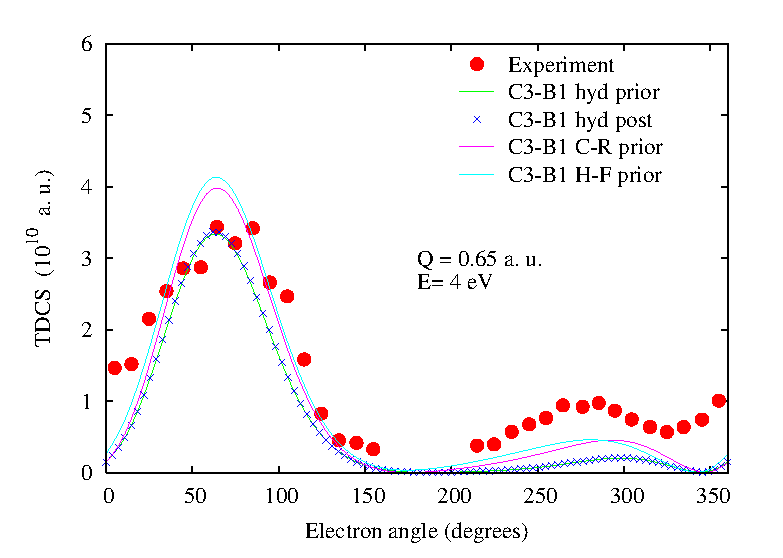
\includegraphics[width=0.7\textwidth]{compara_c3}
  \caption{TDCS for $E_{e}=4$ eV and $Q=0.65$~a.u. in the CDW-B1 approximation for different representation of the initial and final states.}
\end{figure}

\begin{figure}[!htpb]
  \label{F:comparacdw}
  \centering
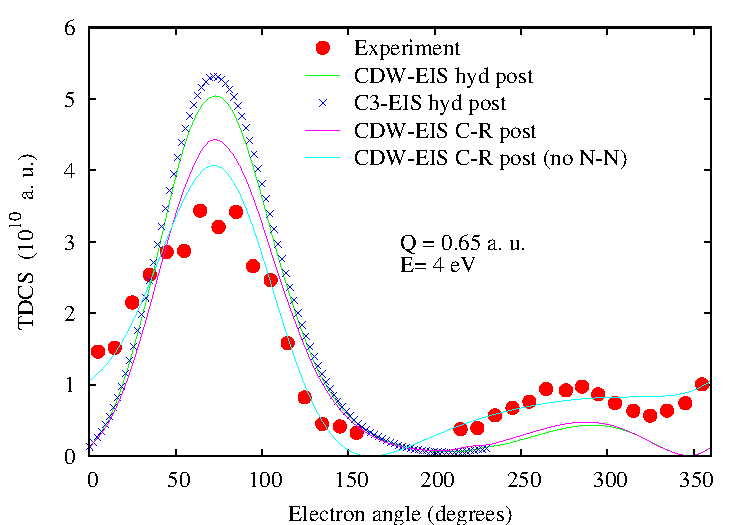
\includegraphics[width=0.7\textwidth]{compara_cdw}
  \caption{TDCS for $E_{e}=4$ eV and $Q=0.65$~a.u. in the CDW-EIS approximation for different representation of the initial and final states.}
\end{figure}

\section{Effective charge dependency}
\label{S:effec-charg-depen}

In the CDW-EIS approximation we studied the effect of the nuclear-nuclear interaction. We described it as a Coulomb force of charge ZN. As observed before, the best description is given for negligible internuclear interaction. 

\begin{figure}[!htpb]
  \centering
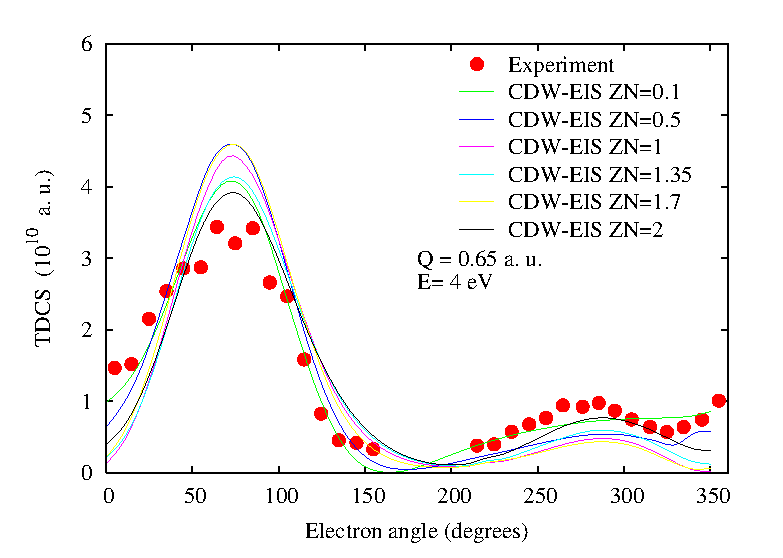
\includegraphics[width=0.7\textwidth]{compara_cdwZN}
  \caption{TDCS for $E_{e}=4$ eV and $Q=0.65$~a.u. in the CDW-EIS approximation for different charges of the internuclear interaction.}
  \label{F:compara-cdwZN}
\end{figure}


\section{Inclusion of experimental uncertainties}
\label{S:inclu-exper-uncer}

Here we want to discuss how to do the convolution over the temperature. The result is very different if we convolute the cross section
${d \sigma}/{d \Omega_{P} d E_{e} d \Omega_{e}}$ or $ {d \sigma}/{d \bm{Q} d E_{e} d \Omega_{e}} $ because the factor $1/Q$ that relates them gives different weights to cross sections for small and large $Q$ in each case.

The main assumption is that the target atom in the initial state is not at rest but has a random momentum $K_{i}$ with probability given by a Gauss distribution in each direction
\begin{equation}\label{Q:gauss-distr}
 p(K_{i}) dK_{i} = \frac{1}{\sqrt{2 \pi \sigma_{i}^2}} \exp (-K_{i}^{2} / 2\sigma_{i}^{2}) dK_{i} \, .  
\end{equation}
%
 The standard deviation $\sigma$ is related to the jet temperature by $\sigma=\sqrt{M_{T} k_{B} T}$, where $k_{B}$ is Boltzmann's constant. This relation gives $\sigma = 0.15$~a.u. for $T=1^{\circ}$K.

If we consider negligible the uncertainty in the determination of the electron momentum $\bm{k}$, we can carry the uncertainty in the atom initial momentum over to the momentum transfer $\bm{Q}=\bm{K}_{R}+ \bm{k}$

Thus, in the case of perfect experimental conditions for the electron, the experimental cross section is determined from the number of events such that the  momentum of the recoil is $\bm{K}_{R}=\bm{Q}+\bm{k}$. The observed cross section for a nominal momentum transfer $\bm{Q}_{0}$ is obtained from the convolution over the uncertainties:

\[
\frac{d \sigma}{d \bm{Q}_{0} d E_{e} d \Omega_{e}} = \int_{\Delta \bm{Q}} \frac{d \sigma}{d \bm{Q} d E_{e} d \Omega_{e}}\, p( \bm{Q} - \bm{Q}_{0} ) \, d \bm{Q}
\]

Now, let's consider that the two perpendicular components present the same uncertainty while the perpendicular is perfectly determined (much smaller deviation $\sigma$ in real life). Then, the two-dimensional distribution can be rewritten for the magnitude of the perpendicular component and one angle


\begin{eqnarray*}
  p(\bm{Q}_{\perp} - \bm{Q}_{{\perp},0}) d\bm{Q}_{\perp} &=&  p(Q_{x}-Q_{x,0}) dQ_{x} \, p(Q_{y}-Q_{y,0}) d Q_{y} \\
&=& \frac{1}{2 \pi \sigma^2} \, \exp \left[{- \left|\bm{Q}_{\perp} - \bm{Q}_{{\perp},0}\right|^{2} / 2\sigma^{2}} \right] Q_{\perp} \, dQ_{\perp} \, d \varphi_{Qe} \, .
\end{eqnarray*}



In conclusion, we have to add the experimental results in the following way

\begin{align}\label{Q:convol-exact}
 \frac{d \sigma}{d \bm{Q}_{\perp , 0} d E_{e} d \Omega_{e}} &= \int_{\Delta \bm{Q}} \frac{d \sigma}{d \bm{Q}_{\perp} d E_{e} d \Omega_{e}}\, p( \bm{Q}_{\perp} ) \, d \bm{Q}_{\perp} \nonumber \\
&= \frac{1}{2 \pi \sigma^{2}} \int_{0}^{\infty} Q_{\perp} \, d Q_{\perp} \int_{0}^{2 \pi}  \frac{d \sigma}{ d \bm{Q}_{\perp} d E_{e} d \Omega_{e}}\, e^{- \left|\bm{Q}_{\perp} - \bm{Q}_{{\perp},0}\right|^{2} / 2\sigma^{2}} \, d \varphi_{Q_{\perp}} \nonumber \\
&= \frac{1}{2 \pi \sigma^{2}} \int_{0}^{\infty} e^{- \left({Q}^{2}_{\perp} + {Q}^{2}_{{\perp},0}\right)^{2} / 2\sigma^{2}}  Q_{\perp} \, d Q_{\perp} \int_{0}^{2 \pi}  \frac{d \sigma}{ d \bm{Q}_{\perp}}\, e^{{Q}_{\perp} {Q}_{{\perp},0} \cos{\varphi}/\sigma^{2}} \, d \varphi_{Q_{\perp}}
\nonumber \\
&= \frac{e^{- Q^{2}_{{\perp},0} / 2\sigma^{2}} } {\sqrt{2 \pi \sigma^{2}}} \int_{0}^{\infty}   \frac{e^{- Q^{2}_{{\perp}} / 2\sigma^{2}} } {\sqrt{2 \pi \sigma^{2}}} \, Q_{\perp} d Q_{\perp} \int_{0}^{2 \pi}  \frac{d \sigma}{ d \bm{Q}_{\perp}}\, e^{{Q}_{\perp} {Q}_{{\perp},0} \cos{\varphi}/\sigma^{2}} \, d \varphi_{Q_{\perp}}
\nonumber \\
&= 2\, p(Q_{\perp,0},\sigma) \int_{0}^{\infty}  p(Q_{\perp},\sigma) \, Q_{\perp} d Q_{\perp} \int_{0}^{\pi}  \frac{d \sigma}{ d \bm{Q}_{\perp}}\, e^{{Q}_{\perp} {Q}_{{\perp},0} \cos{\varphi}/\sigma^{2}} \, d \varphi_{Q_{\perp}} 
\end{align}
%
where $p(x,\sigma)$ is the Gauss distribution of Eq. \ref{Q:gauss-distr}.



\subsection*{Peaking approximation at $\varphi=0$}

Now, the roughest approximation for the integral on the azimuthal angle $\varphi$ would be to consider that the cross section is independent of it and take it out of the integral. In this way we obtain

\begin{eqnarray}\label{Q:Aprox-0-convo}
\frac{d \sigma}{d \bm{Q}_{\perp , 0} d E_{e} d \Omega_{e}} 
&=& p(Q_{\perp,0},\sigma) \int_{0}^{\infty}  p(Q_{\perp},\sigma) \, \left(Q_{\perp} \frac{d \sigma}{ d \bm{Q}_{\perp}}(Q_{\perp})\right)_{\varphi=0} \, d Q_{\perp} \int_{0}^{2 \pi} \, e^{{Q}_{\perp} {Q}_{{\perp},0} \cos{\varphi}/\sigma^{2}} \, d \varphi_{Q_{\perp}} 
\nonumber \\
&=& p(Q_{\perp,0},\sigma) \int_{0}^{\infty}  p(Q_{\perp},\sigma) \, \left(Q_{\perp} \frac{d \sigma}{ d \bm{Q}_{\perp}}(Q_{\perp})\right)_{\varphi=0} \, d Q_{\perp} \left[ 2 \pi \,I^{B}_{0}(Q_{\perp} Q_{\perp,0}/\sigma^{2}) \right]
\end{eqnarray}
%
where $I^{B}_{0}$ is the Modified Bessel function (see chapter 9, page 376 of \cite{Abramow1972_HOM}).


\begin{figure}[!htpb]
  \centering
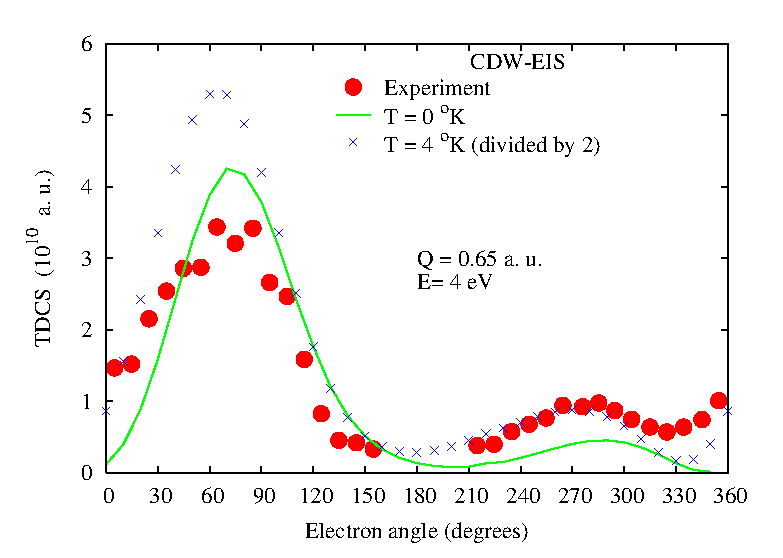
\includegraphics[width=0.7\textwidth]{cdwe4q065t4_app0}
  \caption{TDCS for $E_{e}=4$ eV and $Q=0.65$~a.u. in the CDW-EIS approximation for temperature convolution in approximation 0.}
  \label{F:cdwe4q065t4_app0}
\end{figure}


\subsection*{Peaking approximation at $\varphi=0$ and $\varphi=\pi$}

The next level of approximation would be to consider separately the coplanar $(\varphi=0)$ and anti-coplanar $(\varphi=\pi)$ directions.

\begin{flalign}\label{Q:Aprox-1-convo}
 \frac{d \sigma}{d \bm{Q}_{\perp , 0} d E_{e} d \Omega_{e}} =&
 p(Q_{\perp,0},\sigma) \int_{0}^{\infty}  p(Q_{\perp},\sigma) \, d Q_{\perp} \times 
\\
& \left[ \left( 2 \pi Q_{\perp} \frac{d \sigma}{ d \bm{Q}_{\perp}} \right)_{\varphi=0} \, \,I_{0} \left( \frac{Q_{\perp} Q_{\perp,0}}{\sigma^{2}} \right) + 
 \left( 2 \pi Q_{\perp} \frac{d \sigma}{ d \bm{Q}_{\perp}} \right)_{\varphi=\pi} \,I_{0}\left( -\frac{Q_{\perp} Q_{\perp,0}}{\sigma^{2}} \right)\right] \nonumber
\end{flalign}
%
where we have defined 

\begin{equation}\label{Q:I0}
  I_{0}(x)= \frac{1}{\pi} \, \int_{0}^{\pi/2} e^{x \, \cos(\varphi)} \, d \varphi
\end{equation}
%
such that $I^{B}_{0}(x) = I_{0}(x) + I_{0}(-x)$.


\begin{figure}[!htpb]
  \centering
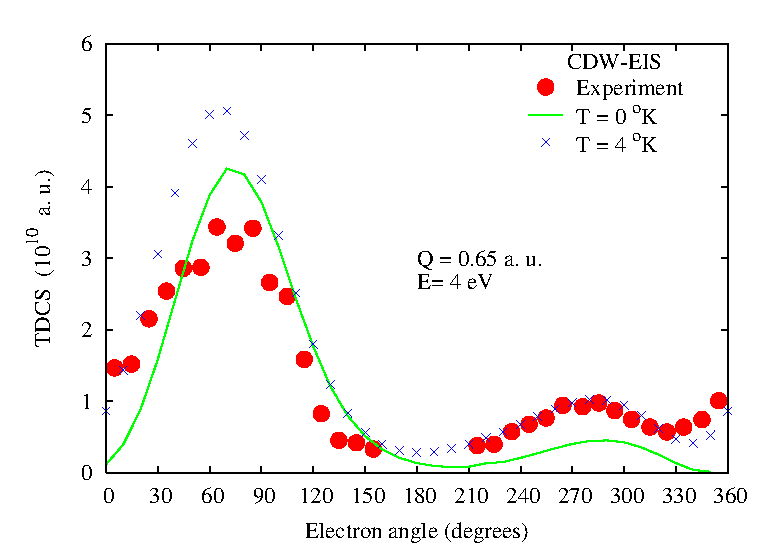
\includegraphics[width=0.7\textwidth]{cdwe4q065t4_app1}
  \caption{TDCS for $E_{e}=4$ eV and $Q=0.65$~a.u. in the CDW-EIS approximation for temperature convolution in approximation 0.}
  \label{F:cdwe4q065t4_app1}
\end{figure}

The virtue of these approximations is that not out-of-the-plane calculations are needed.


\subsection{Anisotropic resolution in cylindrical coordinates}
\label{S:anis-resol-cylin-coord}

Sebasti\'{a}n derived the following expresion for $\sigma_{x}\neq \sigma_{y}$

\[
\left\langle \frac{d \sigma }{dQ_{\perp}} \right\rangle = \frac{1}{2\pi
  \sigma_{x} \sigma_{y}} \int_{0}^{\infty} dQ_{\perp} \int_{0}^{\pi} d\varphi
\left(p (Q_{\perp },\varphi ,Q_{0\perp}) + p(Q_{\perp },2\pi -\varphi
  ,Q_{0\perp}) \right)
\]

\begin{eqnarray*}
  p(Q_{\perp },\varphi ,Q_{0}) &=&\exp \left[ -\frac{(Q_{\perp }^{2}\cos
      ^{2}\varphi +Q_{0\perp }^{2}\cos ^{2}\varphi _{0}-2Q_{\perp }Q_{0\perp }\cos
      \varphi \cos \varphi _{0})}{2\sigma _{x}^{2}} \right] 
  \\
  && \left.  - \frac{(Q_{\perp }^{2} \sin^{2}\varphi +Q_{0\perp }^{2}\sin ^{2}\varphi _{0}-2Q_{\perp }Q_{0\perp }\sin
      \varphi \sin \varphi _{0})}{2\sigma _{y}^{2}}\right]  \\
  p(Q_{\perp },2\pi -\varphi ,Q_{0}) 
  &=&\exp \left[ - \frac{(Q_{\perp }^{2}\cos^{2} \left( 2\pi -\varphi \right) +Q_{0\perp }^{2} \cos ^{2}\varphi_{0} - 
      2Q_{\perp }Q_{0\perp }\cos \left( 2\pi -\varphi \right) \cos \varphi_{0})} {2\sigma_{x}^{2}} \right.  \\
  && \left. - \frac{(Q_{\perp }^{2}\sin ^{2}\left( 2\pi -\varphi \right) + Q_{0\perp }^{2}\sin ^{2}\varphi _{0}-2Q_{\perp }Q_{0\perp } 
      \sin\left( 2\pi -\varphi \right) \sin \varphi _{0})}{2\sigma _{y}^{2}}\right] 
\end{eqnarray*}

If $\sigma_{x} = \sigma_{y}=\sigma $ then these last expressions reduce to,

\begin{eqnarray*}
p(Q_{\perp },\varphi ,Q_{0}) &=&\exp \left[ -\frac{(Q_{\perp }^{2}+Q_{0\perp}^{2}-2Q_{\perp} Q_{0\perp }\cos \varphi \cos \varphi _{0}-2Q_{\perp} Q_{0\perp }\sin \varphi \sin \varphi _{0})}{2\sigma ^{2}}\right]  \\
p(Q_{\perp },2\pi -\varphi ,Q_{0}) &=&\exp \left[ -\frac{(Q_{\perp}^{2}+Q_{0\perp }^{2}-2Q_{\perp }Q_{0\perp }\cos \left( 2\pi -\varphi \right) \cos \varphi _{0}-2Q_{\perp }Q_{0\perp }\sin \left( 2\pi -\varphi \right) \sin \varphi _{0})}{2\sigma ^{2}}\right] 
\end{eqnarray*}


\subsection{Anisotropic resolution in cartesian coordinates} 
\label{S:anis-resol-carte-coord}

Starting from the general expresion for a gaussian uncertainty in the momentum
\[
\frac{d \sigma}{d \bm{Q}_{0} d E_{e} d \Omega_{e}} = \int_{\Delta
  \bm{Q}} \frac{d \sigma}{d \bm{Q} d E_{e} d \Omega_{e}}\, p_{x}( Q_{x}- Q_{0,x} ) p_{y}( Q_{y}- Q_{0,y} ) \, d Q_{x} d Q_{y}
\]
with
\[
 p_{i}(K_{i}) dK_{i} = \frac{1}{\sqrt{2 \pi \sigma_{i}^2}} \exp (-K_{i}^{2} / 2\sigma_{i}^{2}) dK_{i} \, .  
\]

In order to perform these convolutions we will integrate numerically these expresions interpolating the cross sections using splines in one direction and taking the average of the values in the other. A good check will be to choose first one and then the other direcion for the interpolation.

\subsection{Results for exact convolution}
\label{S:resul-exact-convol}

These are the results obtained with the two-dimensional integral in the angle $\varphi$ and the momentum transfer $Q_{\perp}$ given by (\ref{Q:convol-exact}), using a Simpson routine with step $\Delta \varphi = 10^{\circ}$ and $\Delta Q_{\perp}=0.05$ for $0.05 \le Q_{\perp} \le 1.55$~a.u.  The use of a Simpson routine . 

\begin{figure}[!htpb]
  \centering
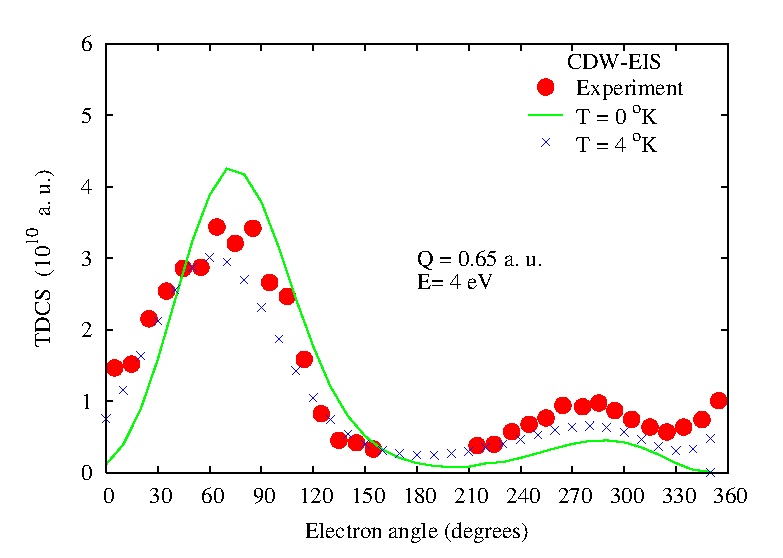
\includegraphics[width=0.7\textwidth]{cdwe4q065t4_app2}
  \caption{TDCS for $E_{e}=4$ eV and $Q=0.65$~a.u. in the CDW-EIS approximation for temperature convolution with T$=4^{\circ}$K.}
  \label{F:cdwe4q065t4_app2}
\end{figure}

\begin{figure}[!htpb]
  \centering
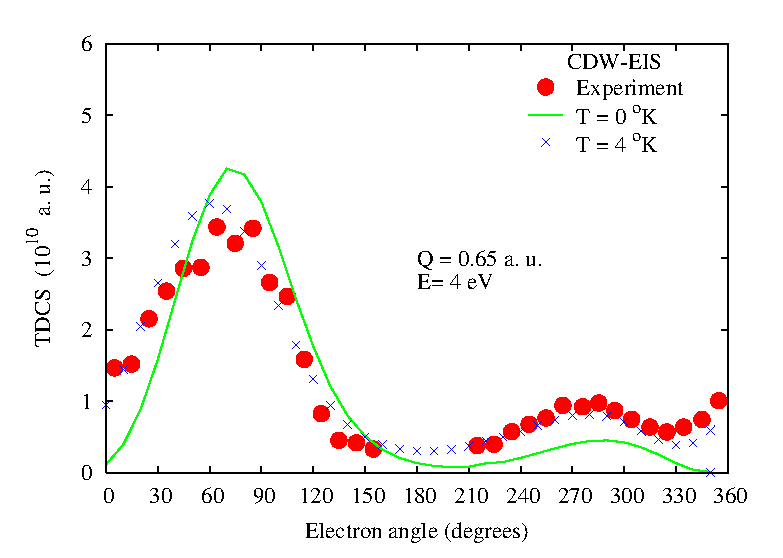
\includegraphics[width=0.7\textwidth]{cdwe4q065t4_app2_125}
  \caption{TDCS for $E_{e}=4$ eV and $Q=0.65$~a.u. in the CDW-EIS approximation for temperature convolution, scaled by 1.25.}
  \label{F:cdwe4q065t4_app2_125}
\end{figure}

These calculations were performed with $Z_{N}=1.354$ though the impact parameter dependence observed for the CTMC seems to indicate that $Z_{N}=1$ is more adequate.  As observed in figure \ref{F:compara-cdwZN} the binary peak is slightly higher for $Z_{N}=1.0$. 


%%% Local Variables: 
%%% mode: latex
%%% TeX-master: "main"
%%% End: 



% %JF: Para usar con bibtex
% \bibliographystyle{apalike}
% \bibliography{bib}
% \bibliographystyle{amsalpha}

%JF: Para usar con biblatex
\printbibliography 

\end{document}

